\documentclass[twoside]{book}

% Packages required by doxygen
\usepackage{calc}
\usepackage{doxygen}
\usepackage{graphicx}
\usepackage[utf8]{inputenc}
\usepackage{makeidx}
\usepackage{multicol}
\usepackage{multirow}
\usepackage{textcomp}
\usepackage[table]{xcolor}

% Font selection
\usepackage[T1]{fontenc}
\usepackage{mathptmx}
\usepackage[scaled=.90]{helvet}
\usepackage{courier}
\usepackage{amssymb}
\usepackage{sectsty}
\renewcommand{\familydefault}{\sfdefault}
\allsectionsfont{%
  \fontseries{bc}\selectfont%
  \color{darkgray}%
}
\renewcommand{\DoxyLabelFont}{%
  \fontseries{bc}\selectfont%
  \color{darkgray}%
}

% Page & text layout
\usepackage{geometry}
\geometry{%
  a4paper,%
  top=2.5cm,%
  bottom=2.5cm,%
  left=2.5cm,%
  right=2.5cm%
}
\tolerance=750
\hfuzz=15pt
\hbadness=750
\setlength{\emergencystretch}{15pt}
\setlength{\parindent}{0cm}
\setlength{\parskip}{0.2cm}
\makeatletter
\renewcommand{\paragraph}{%
  \@startsection{paragraph}{4}{0ex}{-1.0ex}{1.0ex}{%
    \normalfont\normalsize\bfseries\SS@parafont%
  }%
}
\renewcommand{\subparagraph}{%
  \@startsection{subparagraph}{5}{0ex}{-1.0ex}{1.0ex}{%
    \normalfont\normalsize\bfseries\SS@subparafont%
  }%
}
\makeatother

% Headers & footers
\usepackage{fancyhdr}
\pagestyle{fancyplain}
\fancyhead[LE]{\fancyplain{}{\bfseries\thepage}}
\fancyhead[CE]{\fancyplain{}{}}
\fancyhead[RE]{\fancyplain{}{\bfseries\leftmark}}
\fancyhead[LO]{\fancyplain{}{\bfseries\rightmark}}
\fancyhead[CO]{\fancyplain{}{}}
\fancyhead[RO]{\fancyplain{}{\bfseries\thepage}}
\fancyfoot[LE]{\fancyplain{}{}}
\fancyfoot[CE]{\fancyplain{}{}}
\fancyfoot[RE]{\fancyplain{}{\bfseries\scriptsize Generated on Tue Feb 28 2017 15\-:52\-:38 for Variant\-D\-B\-S\-C\-A\-N by Doxygen }}
\fancyfoot[LO]{\fancyplain{}{\bfseries\scriptsize Generated on Tue Feb 28 2017 15\-:52\-:38 for Variant\-D\-B\-S\-C\-A\-N by Doxygen }}
\fancyfoot[CO]{\fancyplain{}{}}
\fancyfoot[RO]{\fancyplain{}{}}
\renewcommand{\footrulewidth}{0.4pt}
\renewcommand{\chaptermark}[1]{%
  \markboth{#1}{}%
}
\renewcommand{\sectionmark}[1]{%
  \markright{\thesection\ #1}%
}

% Indices & bibliography
\usepackage{natbib}
\usepackage[titles]{tocloft}
\setcounter{tocdepth}{3}
\setcounter{secnumdepth}{5}
\makeindex

% Hyperlinks (required, but should be loaded last)
\usepackage{ifpdf}
\ifpdf
  \usepackage[pdftex,pagebackref=true]{hyperref}
\else
  \usepackage[ps2pdf,pagebackref=true]{hyperref}
\fi
\hypersetup{%
  colorlinks=true,%
  linkcolor=blue,%
  citecolor=blue,%
  unicode%
}

% Custom commands
\newcommand{\clearemptydoublepage}{%
  \newpage{\pagestyle{empty}\cleardoublepage}%
}


%===== C O N T E N T S =====

\begin{document}

% Titlepage & ToC
\hypersetup{pageanchor=false}
\pagenumbering{roman}
\begin{titlepage}
\vspace*{7cm}
\begin{center}%
{\Large Variant\-D\-B\-S\-C\-A\-N }\\
\vspace*{1cm}
{\large Generated by Doxygen 1.8.6}\\
\vspace*{0.5cm}
{\small Tue Feb 28 2017 15:52:38}\\
\end{center}
\end{titlepage}
\clearemptydoublepage
\tableofcontents
\clearemptydoublepage
\pagenumbering{arabic}
\hypersetup{pageanchor=true}

%--- Begin generated contents ---
\chapter{Data Structure Index}
\section{Data Structures}
Here are the data structures with brief descriptions\-:\begin{DoxyCompactList}
\item\contentsline{section}{\hyperlink{structRTree_1_1Branch}{R\-Tree$<$ D\-A\-T\-A\-T\-Y\-P\-E, E\-L\-E\-M\-T\-Y\-P\-E, N\-U\-M\-D\-I\-M\-S, E\-L\-E\-M\-T\-Y\-P\-E\-R\-E\-A\-L, T\-M\-A\-X\-N\-O\-D\-E\-S, T\-M\-I\-N\-N\-O\-D\-E\-S $>$\-::\-Branch} }{\pageref{structRTree_1_1Branch}}{}
\item\contentsline{section}{\hyperlink{structdataElem}{data\-Elem} }{\pageref{structdataElem}}{}
\item\contentsline{section}{\hyperlink{classDBScan}{D\-B\-Scan} }{\pageref{classDBScan}}{}
\item\contentsline{section}{\hyperlink{structdensityStruct}{density\-Struct} }{\pageref{structdensityStruct}}{}
\item\contentsline{section}{\hyperlink{structexperiment}{experiment} }{\pageref{structexperiment}}{}
\item\contentsline{section}{\hyperlink{classRTree_1_1Iterator}{R\-Tree$<$ D\-A\-T\-A\-T\-Y\-P\-E, E\-L\-E\-M\-T\-Y\-P\-E, N\-U\-M\-D\-I\-M\-S, E\-L\-E\-M\-T\-Y\-P\-E\-R\-E\-A\-L, T\-M\-A\-X\-N\-O\-D\-E\-S, T\-M\-I\-N\-N\-O\-D\-E\-S $>$\-::\-Iterator} \\*\hyperlink{classRTree_1_1Iterator}{Iterator} is not remove safe }{\pageref{classRTree_1_1Iterator}}{}
\item\contentsline{section}{\hyperlink{structRTree_1_1ListNode}{R\-Tree$<$ D\-A\-T\-A\-T\-Y\-P\-E, E\-L\-E\-M\-T\-Y\-P\-E, N\-U\-M\-D\-I\-M\-S, E\-L\-E\-M\-T\-Y\-P\-E\-R\-E\-A\-L, T\-M\-A\-X\-N\-O\-D\-E\-S, T\-M\-I\-N\-N\-O\-D\-E\-S $>$\-::\-List\-Node} \\*A link list of nodes for reinsertion after a delete operation }{\pageref{structRTree_1_1ListNode}}{}
\item\contentsline{section}{\hyperlink{structMPBRect}{M\-P\-B\-Rect} }{\pageref{structMPBRect}}{}
\item\contentsline{section}{\hyperlink{structRTree_1_1Node}{R\-Tree$<$ D\-A\-T\-A\-T\-Y\-P\-E, E\-L\-E\-M\-T\-Y\-P\-E, N\-U\-M\-D\-I\-M\-S, E\-L\-E\-M\-T\-Y\-P\-E\-R\-E\-A\-L, T\-M\-A\-X\-N\-O\-D\-E\-S, T\-M\-I\-N\-N\-O\-D\-E\-S $>$\-::\-Node} \\*\hyperlink{structRTree_1_1Node}{Node} for each branch level }{\pageref{structRTree_1_1Node}}{}
\item\contentsline{section}{\hyperlink{structRTree_1_1PartitionVars}{R\-Tree$<$ D\-A\-T\-A\-T\-Y\-P\-E, E\-L\-E\-M\-T\-Y\-P\-E, N\-U\-M\-D\-I\-M\-S, E\-L\-E\-M\-T\-Y\-P\-E\-R\-E\-A\-L, T\-M\-A\-X\-N\-O\-D\-E\-S, T\-M\-I\-N\-N\-O\-D\-E\-S $>$\-::\-Partition\-Vars} \\*Variables for finding a split partition }{\pageref{structRTree_1_1PartitionVars}}{}
\item\contentsline{section}{\hyperlink{structQueryRect}{Query\-Rect} }{\pageref{structQueryRect}}{}
\item\contentsline{section}{\hyperlink{structRTree_1_1Rect}{R\-Tree$<$ D\-A\-T\-A\-T\-Y\-P\-E, E\-L\-E\-M\-T\-Y\-P\-E, N\-U\-M\-D\-I\-M\-S, E\-L\-E\-M\-T\-Y\-P\-E\-R\-E\-A\-L, T\-M\-A\-X\-N\-O\-D\-E\-S, T\-M\-I\-N\-N\-O\-D\-E\-S $>$\-::\-Rect} \\*Minimal bounding rectangle (n-\/dimensional) }{\pageref{structRTree_1_1Rect}}{}
\item\contentsline{section}{\hyperlink{structRect}{Rect} }{\pageref{structRect}}{}
\item\contentsline{section}{\hyperlink{classRTFileStream}{R\-T\-File\-Stream} }{\pageref{classRTFileStream}}{}
\item\contentsline{section}{\hyperlink{classRTree}{R\-Tree$<$ D\-A\-T\-A\-T\-Y\-P\-E, E\-L\-E\-M\-T\-Y\-P\-E, N\-U\-M\-D\-I\-M\-S, E\-L\-E\-M\-T\-Y\-P\-E\-R\-E\-A\-L, T\-M\-A\-X\-N\-O\-D\-E\-S, T\-M\-I\-N\-N\-O\-D\-E\-S $>$} }{\pageref{classRTree}}{}
\item\contentsline{section}{\hyperlink{structschedInfo}{sched\-Info} }{\pageref{structschedInfo}}{}
\item\contentsline{section}{\hyperlink{classSchedule}{Schedule} }{\pageref{classSchedule}}{}
\item\contentsline{section}{\hyperlink{structRTree_1_1Iterator_1_1StackElement}{R\-Tree$<$ D\-A\-T\-A\-T\-Y\-P\-E, E\-L\-E\-M\-T\-Y\-P\-E, N\-U\-M\-D\-I\-M\-S, E\-L\-E\-M\-T\-Y\-P\-E\-R\-E\-A\-L, T\-M\-A\-X\-N\-O\-D\-E\-S, T\-M\-I\-N\-N\-O\-D\-E\-S $>$\-::\-Iterator\-::\-Stack\-Element} }{\pageref{structRTree_1_1Iterator_1_1StackElement}}{}
\end{DoxyCompactList}

\chapter{File Index}
\section{File List}
Here is a list of all files with brief descriptions\-:\begin{DoxyCompactList}
\item\contentsline{section}{\hyperlink{c__test__prog_8cpp}{c\-\_\-test\-\_\-prog.\-cpp} }{\pageref{c__test__prog_8cpp}}{}
\item\contentsline{section}{\hyperlink{c__test__prog_8h}{c\-\_\-test\-\_\-prog.\-h} }{\pageref{c__test__prog_8h}}{}
\item\contentsline{section}{\hyperlink{DBScan_8cpp}{D\-B\-Scan.\-cpp} }{\pageref{DBScan_8cpp}}{}
\item\contentsline{section}{\hyperlink{DBScan_8h}{D\-B\-Scan.\-h} }{\pageref{DBScan_8h}}{}
\item\contentsline{section}{\hyperlink{globals_8h}{globals.\-h} }{\pageref{globals_8h}}{}
\item\contentsline{section}{\hyperlink{main_8cpp}{main.\-cpp} }{\pageref{main_8cpp}}{}
\item\contentsline{section}{\hyperlink{prototypes_8h}{prototypes.\-h} }{\pageref{prototypes_8h}}{}
\item\contentsline{section}{\hyperlink{RTree_8h}{R\-Tree.\-h} }{\pageref{RTree_8h}}{}
\item\contentsline{section}{\hyperlink{schedule_8cpp}{schedule.\-cpp} }{\pageref{schedule_8cpp}}{}
\item\contentsline{section}{\hyperlink{schedule_8h}{schedule.\-h} }{\pageref{schedule_8h}}{}
\item\contentsline{section}{\hyperlink{structs_8h}{structs.\-h} }{\pageref{structs_8h}}{}
\item\contentsline{section}{\hyperlink{tree__functions_8cpp}{tree\-\_\-functions.\-cpp} }{\pageref{tree__functions_8cpp}}{}
\end{DoxyCompactList}

\chapter{Data Structure Documentation}
\hypertarget{structRTree_1_1Branch}{\section{R\-Tree$<$ D\-A\-T\-A\-T\-Y\-P\-E, E\-L\-E\-M\-T\-Y\-P\-E, N\-U\-M\-D\-I\-M\-S, E\-L\-E\-M\-T\-Y\-P\-E\-R\-E\-A\-L, T\-M\-A\-X\-N\-O\-D\-E\-S, T\-M\-I\-N\-N\-O\-D\-E\-S $>$\-:\-:Branch Struct Reference}
\label{structRTree_1_1Branch}\index{R\-Tree$<$ D\-A\-T\-A\-T\-Y\-P\-E, E\-L\-E\-M\-T\-Y\-P\-E, N\-U\-M\-D\-I\-M\-S, E\-L\-E\-M\-T\-Y\-P\-E\-R\-E\-A\-L, T\-M\-A\-X\-N\-O\-D\-E\-S, T\-M\-I\-N\-N\-O\-D\-E\-S $>$\-::\-Branch@{R\-Tree$<$ D\-A\-T\-A\-T\-Y\-P\-E, E\-L\-E\-M\-T\-Y\-P\-E, N\-U\-M\-D\-I\-M\-S, E\-L\-E\-M\-T\-Y\-P\-E\-R\-E\-A\-L, T\-M\-A\-X\-N\-O\-D\-E\-S, T\-M\-I\-N\-N\-O\-D\-E\-S $>$\-::\-Branch}}
}


{\ttfamily \#include \char`\"{}R\-Tree.\-h\char`\"{}}



Collaboration diagram for R\-Tree$<$ D\-A\-T\-A\-T\-Y\-P\-E, E\-L\-E\-M\-T\-Y\-P\-E, N\-U\-M\-D\-I\-M\-S, E\-L\-E\-M\-T\-Y\-P\-E\-R\-E\-A\-L, T\-M\-A\-X\-N\-O\-D\-E\-S, T\-M\-I\-N\-N\-O\-D\-E\-S $>$\-:\-:Branch\-:\nopagebreak
\begin{figure}[H]
\begin{center}
\leavevmode
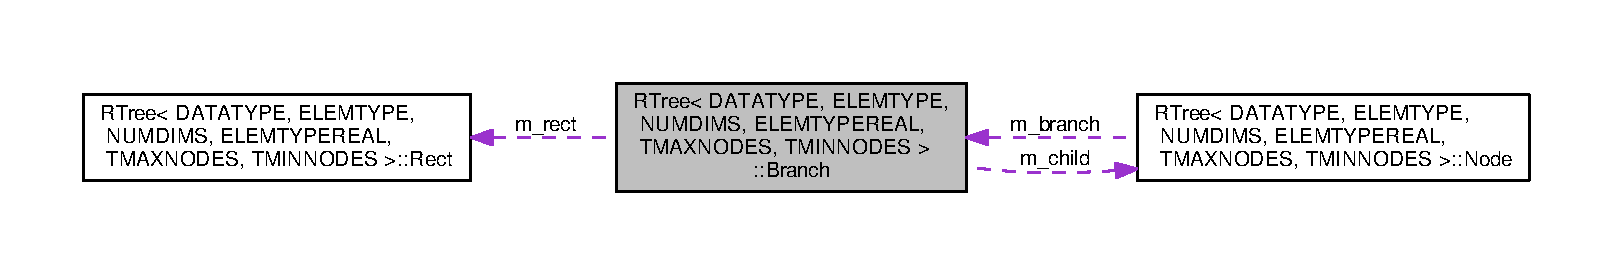
\includegraphics[width=350pt]{structRTree_1_1Branch__coll__graph}
\end{center}
\end{figure}
\subsection*{Data Fields}
\begin{DoxyCompactItemize}
\item 
\hyperlink{structRTree_1_1Rect}{Rect} \hyperlink{structRTree_1_1Branch_a7e98e0d7fb6afd18ec243450b22d9abe}{m\-\_\-rect}
\begin{DoxyCompactList}\small\item\em Bounds. \end{DoxyCompactList}\item 
\hyperlink{structRTree_1_1Node}{Node} $\ast$ \hyperlink{structRTree_1_1Branch_aa15f22000d06c726372eb84f46db0fa0}{m\-\_\-child}
\begin{DoxyCompactList}\small\item\em Child node. \end{DoxyCompactList}\item 
D\-A\-T\-A\-T\-Y\-P\-E \hyperlink{structRTree_1_1Branch_afc1aee31a1a62ad4e800a536a3a9d665}{m\-\_\-data}
\begin{DoxyCompactList}\small\item\em Data Id or Ptr. \end{DoxyCompactList}\end{DoxyCompactItemize}


\subsection{Detailed Description}
\subsubsection*{template$<$class D\-A\-T\-A\-T\-Y\-P\-E, class E\-L\-E\-M\-T\-Y\-P\-E, int N\-U\-M\-D\-I\-M\-S, class E\-L\-E\-M\-T\-Y\-P\-E\-R\-E\-A\-L = E\-L\-E\-M\-T\-Y\-P\-E, int T\-M\-A\-X\-N\-O\-D\-E\-S = 8, int T\-M\-I\-N\-N\-O\-D\-E\-S = T\-M\-A\-X\-N\-O\-D\-E\-S / 2$>$struct R\-Tree$<$ D\-A\-T\-A\-T\-Y\-P\-E, E\-L\-E\-M\-T\-Y\-P\-E, N\-U\-M\-D\-I\-M\-S, E\-L\-E\-M\-T\-Y\-P\-E\-R\-E\-A\-L, T\-M\-A\-X\-N\-O\-D\-E\-S, T\-M\-I\-N\-N\-O\-D\-E\-S $>$\-::\-Branch}

May be data or may be another subtree The parents level determines this. If the parents level is 0, then this is data 

\subsection{Field Documentation}
\hypertarget{structRTree_1_1Branch_aa15f22000d06c726372eb84f46db0fa0}{\index{R\-Tree\-::\-Branch@{R\-Tree\-::\-Branch}!m\-\_\-child@{m\-\_\-child}}
\index{m\-\_\-child@{m\-\_\-child}!RTree::Branch@{R\-Tree\-::\-Branch}}
\subsubsection[{m\-\_\-child}]{\setlength{\rightskip}{0pt plus 5cm}template$<$class D\-A\-T\-A\-T\-Y\-P\-E, class E\-L\-E\-M\-T\-Y\-P\-E, int N\-U\-M\-D\-I\-M\-S, class E\-L\-E\-M\-T\-Y\-P\-E\-R\-E\-A\-L = E\-L\-E\-M\-T\-Y\-P\-E, int T\-M\-A\-X\-N\-O\-D\-E\-S = 8, int T\-M\-I\-N\-N\-O\-D\-E\-S = T\-M\-A\-X\-N\-O\-D\-E\-S / 2$>$ {\bf Node}$\ast$ {\bf R\-Tree}$<$ D\-A\-T\-A\-T\-Y\-P\-E, E\-L\-E\-M\-T\-Y\-P\-E, N\-U\-M\-D\-I\-M\-S, E\-L\-E\-M\-T\-Y\-P\-E\-R\-E\-A\-L, T\-M\-A\-X\-N\-O\-D\-E\-S, T\-M\-I\-N\-N\-O\-D\-E\-S $>$\-::Branch\-::m\-\_\-child}}\label{structRTree_1_1Branch_aa15f22000d06c726372eb84f46db0fa0}


Child node. 

\hypertarget{structRTree_1_1Branch_afc1aee31a1a62ad4e800a536a3a9d665}{\index{R\-Tree\-::\-Branch@{R\-Tree\-::\-Branch}!m\-\_\-data@{m\-\_\-data}}
\index{m\-\_\-data@{m\-\_\-data}!RTree::Branch@{R\-Tree\-::\-Branch}}
\subsubsection[{m\-\_\-data}]{\setlength{\rightskip}{0pt plus 5cm}template$<$class D\-A\-T\-A\-T\-Y\-P\-E, class E\-L\-E\-M\-T\-Y\-P\-E, int N\-U\-M\-D\-I\-M\-S, class E\-L\-E\-M\-T\-Y\-P\-E\-R\-E\-A\-L = E\-L\-E\-M\-T\-Y\-P\-E, int T\-M\-A\-X\-N\-O\-D\-E\-S = 8, int T\-M\-I\-N\-N\-O\-D\-E\-S = T\-M\-A\-X\-N\-O\-D\-E\-S / 2$>$ D\-A\-T\-A\-T\-Y\-P\-E {\bf R\-Tree}$<$ D\-A\-T\-A\-T\-Y\-P\-E, E\-L\-E\-M\-T\-Y\-P\-E, N\-U\-M\-D\-I\-M\-S, E\-L\-E\-M\-T\-Y\-P\-E\-R\-E\-A\-L, T\-M\-A\-X\-N\-O\-D\-E\-S, T\-M\-I\-N\-N\-O\-D\-E\-S $>$\-::Branch\-::m\-\_\-data}}\label{structRTree_1_1Branch_afc1aee31a1a62ad4e800a536a3a9d665}


Data Id or Ptr. 

\hypertarget{structRTree_1_1Branch_a7e98e0d7fb6afd18ec243450b22d9abe}{\index{R\-Tree\-::\-Branch@{R\-Tree\-::\-Branch}!m\-\_\-rect@{m\-\_\-rect}}
\index{m\-\_\-rect@{m\-\_\-rect}!RTree::Branch@{R\-Tree\-::\-Branch}}
\subsubsection[{m\-\_\-rect}]{\setlength{\rightskip}{0pt plus 5cm}template$<$class D\-A\-T\-A\-T\-Y\-P\-E, class E\-L\-E\-M\-T\-Y\-P\-E, int N\-U\-M\-D\-I\-M\-S, class E\-L\-E\-M\-T\-Y\-P\-E\-R\-E\-A\-L = E\-L\-E\-M\-T\-Y\-P\-E, int T\-M\-A\-X\-N\-O\-D\-E\-S = 8, int T\-M\-I\-N\-N\-O\-D\-E\-S = T\-M\-A\-X\-N\-O\-D\-E\-S / 2$>$ {\bf Rect} {\bf R\-Tree}$<$ D\-A\-T\-A\-T\-Y\-P\-E, E\-L\-E\-M\-T\-Y\-P\-E, N\-U\-M\-D\-I\-M\-S, E\-L\-E\-M\-T\-Y\-P\-E\-R\-E\-A\-L, T\-M\-A\-X\-N\-O\-D\-E\-S, T\-M\-I\-N\-N\-O\-D\-E\-S $>$\-::Branch\-::m\-\_\-rect}}\label{structRTree_1_1Branch_a7e98e0d7fb6afd18ec243450b22d9abe}


Bounds. 



The documentation for this struct was generated from the following file\-:\begin{DoxyCompactItemize}
\item 
\hyperlink{RTree_8h}{R\-Tree.\-h}\end{DoxyCompactItemize}

\hypertarget{structdataElem}{\section{data\-Elem Struct Reference}
\label{structdataElem}\index{data\-Elem@{data\-Elem}}
}


{\ttfamily \#include \char`\"{}structs.\-h\char`\"{}}

\subsection*{Data Fields}
\begin{DoxyCompactItemize}
\item 
double \hyperlink{structdataElem_a1197e353644cfe60181b3257d761a2a3}{x}
\item 
double \hyperlink{structdataElem_a94f94bdba1be4815d4254d4c498baf49}{y}
\end{DoxyCompactItemize}


\subsection{Detailed Description}
2-\/\-D data struct 

\subsection{Field Documentation}
\hypertarget{structdataElem_a1197e353644cfe60181b3257d761a2a3}{\index{data\-Elem@{data\-Elem}!x@{x}}
\index{x@{x}!dataElem@{data\-Elem}}
\subsubsection[{x}]{\setlength{\rightskip}{0pt plus 5cm}double data\-Elem\-::x}}\label{structdataElem_a1197e353644cfe60181b3257d761a2a3}
\hypertarget{structdataElem_a94f94bdba1be4815d4254d4c498baf49}{\index{data\-Elem@{data\-Elem}!y@{y}}
\index{y@{y}!dataElem@{data\-Elem}}
\subsubsection[{y}]{\setlength{\rightskip}{0pt plus 5cm}double data\-Elem\-::y}}\label{structdataElem_a94f94bdba1be4815d4254d4c498baf49}


The documentation for this struct was generated from the following file\-:\begin{DoxyCompactItemize}
\item 
\hyperlink{structs_8h}{structs.\-h}\end{DoxyCompactItemize}

\hypertarget{classDBScan}{\section{D\-B\-Scan Class Reference}
\label{classDBScan}\index{D\-B\-Scan@{D\-B\-Scan}}
}


{\ttfamily \#include \char`\"{}D\-B\-Scan.\-h\char`\"{}}



Collaboration diagram for D\-B\-Scan\-:\nopagebreak
\begin{figure}[H]
\begin{center}
\leavevmode
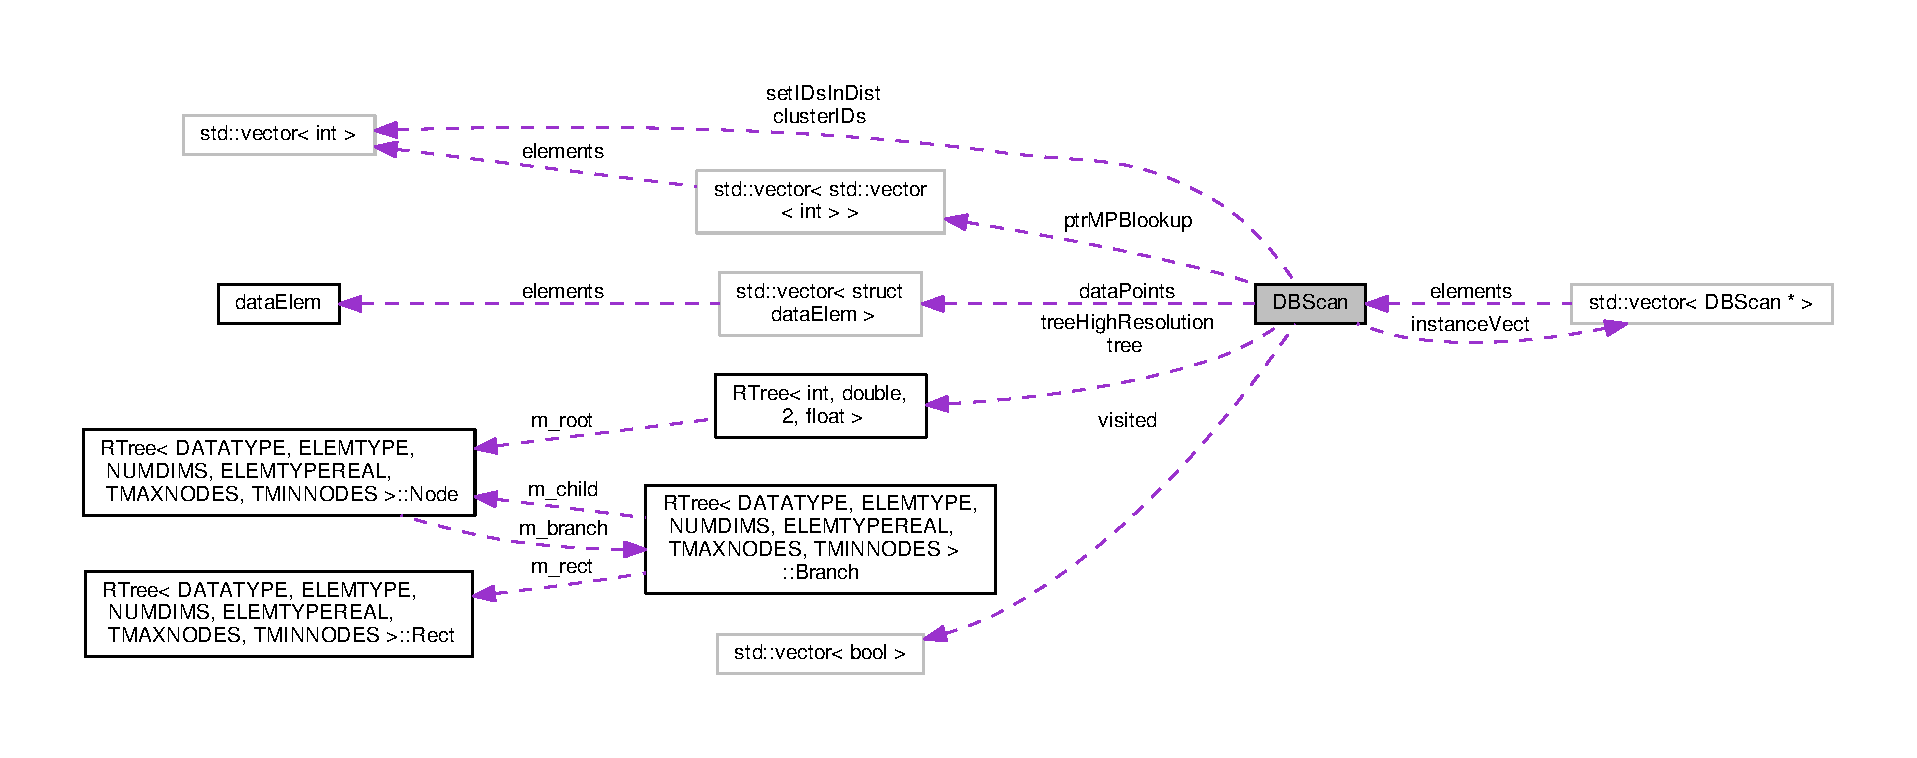
\includegraphics[width=350pt]{classDBScan__coll__graph}
\end{center}
\end{figure}
\subsection*{Public Member Functions}
\begin{DoxyCompactItemize}
\item 
\hyperlink{classDBScan_adbbf078f15acf6fae053d8c288b2e97b}{D\-B\-Scan} (std\-::vector$<$ struct \hyperlink{structdataElem}{data\-Elem} $>$ $\ast$ptr\-Data, double epsilon, int minimum\-Pts, \hyperlink{classRTree}{R\-Tree}$<$ int, double, 2, float $>$ $\ast$index\-Ptr, std\-::vector$<$ std\-::vector$<$ int $>$ $>$ $\ast$ptr\-\_\-\-M\-P\-B\-\_\-lookup, \hyperlink{classRTree}{R\-Tree}$<$ int, double, 2, float $>$ $\ast$high\-Res\-Index)
\item 
void \hyperlink{classDBScan_a55a2c6e7364f2780b2032182d3616bde}{alg\-D\-B\-Scan\-Parallel} ()
\item 
void \hyperlink{classDBScan_a7b7115631994fa281c1dca261973e6a5}{alg\-D\-B\-Scan\-Parallel\-Reuse\-Cluster\-Results} ()
\item 
void \hyperlink{classDBScan_a7d85d5c3c8c06c22dd4c77769baf8104}{generate\-M\-B\-B\-Around\-Cluster} (std\-::vector$<$ int $>$ $\ast$cluster\-Points, double $\ast$M\-B\-B\-\_\-min, double $\ast$M\-B\-B\-\_\-max)
\item 
void \hyperlink{classDBScan_a25383a5401de748f1525cd1aa3705afb}{append\-M\-B\-B\-By\-Epsilon} (double $\ast$M\-B\-B\-\_\-min, double $\ast$M\-B\-B\-\_\-max, double eps)
\item 
void \hyperlink{classDBScan_abaad1d98678fbf99b1c6c67fc3474a3f}{D\-B\-Scan\-Parallel\-M\-P\-B\-S\-T\-U\-M\-P} (int finished\-Instance\-I\-D, bool $\ast$destroyed\-Arr, std\-::vector$<$ int $>$ $\ast$candidates\-To\-Grow\-From)
\item 
void \hyperlink{classDBScan_a31e46e492a6b4a6baa6682f8faf0e2de}{assign\-Points\-To\-Predefined\-Cluster} (int finished\-Instance\-I\-D)
\item 
void \hyperlink{classDBScan_a186a8a9666a4b66bd002e8bf568b0747}{set\-Cluster\-Schedule\-Density} (std\-::vector$<$ int $>$ $\ast$schedule, std\-::vector$<$ int $>$ cluster\-Arr\mbox{[}$\,$\mbox{]}, int num\-Clusters\-In\-Other\-Instance)
\item 
void \hyperlink{classDBScan_ab6eb34d3cad064c121cc156920e62270}{schedule\-Selector} (std\-::vector$<$ int $>$ $\ast$schedule, std\-::vector$<$ int $>$ cluster\-Arr\mbox{[}$\,$\mbox{]}, int num\-Clusters\-In\-Other\-Instance)
\item 
int \hyperlink{classDBScan_ab9f99900ed37f14a166d9c9cc486101a}{get\-D\-B\-Scan\-Num\-Clusters} ()
\end{DoxyCompactItemize}
\subsection*{Static Public Member Functions}
\begin{DoxyCompactItemize}
\item 
static bool \hyperlink{classDBScan_abf662378982ad01ee4b4b0e713887d42}{comparedensity\-Structfn} (const \hyperlink{structdensityStruct}{density\-Struct} \&a, const \hyperlink{structdensityStruct}{density\-Struct} \&b)
\end{DoxyCompactItemize}
\subsection*{Data Fields}
\begin{DoxyCompactItemize}
\item 
std\-::vector$<$ int $>$ \hyperlink{classDBScan_aa363c8aa510fcbd54979f16047d5f0a3}{cluster\-I\-Ds}
\item 
std\-::vector$<$ \hyperlink{classDBScan}{D\-B\-Scan} $\ast$ $>$ \hyperlink{classDBScan_a8270fd572c31089b33fff1e047c00633}{instance\-Vect}
\item 
int \hyperlink{classDBScan_abf8ba9bc0c2b8ff8fab4c9d070f78ec7}{num\-Clusters\-For\-Stats}
\end{DoxyCompactItemize}
\subsection*{Private Member Functions}
\begin{DoxyCompactItemize}
\item 
void \hyperlink{classDBScan_ab919d93ea8f7c4ef59d5112b05ec109b}{initialize\-Visited\-Points} (int size)
\item 
void \hyperlink{classDBScan_ae133eef10ed34bf676d46b1dee6af918}{generate\-M\-B\-B} (struct \hyperlink{structdataElem}{data\-Elem} $\ast$point, double \hyperlink{classDBScan_a9878125297973f29db8b41287e0c9b4d}{distance}, double $\ast$M\-B\-B\-\_\-min, double $\ast$M\-B\-B\-\_\-max)
\item 
bool \hyperlink{classDBScan_a8d882d909001edadc803668743908cc9}{generate\-M\-B\-B\-Normal} (struct \hyperlink{structdataElem}{data\-Elem} $\ast$point, double \hyperlink{classDBScan_a9878125297973f29db8b41287e0c9b4d}{distance}, double $\ast$M\-B\-B\-\_\-min, double $\ast$M\-B\-B\-\_\-max)
\item 
int \hyperlink{classDBScan_a62ea9b65ded887ede6d8b675aef2ce17}{filter\-Candidates\-M\-P\-B} (struct \hyperlink{structdataElem}{data\-Elem} $\ast$point, std\-::vector$<$ int $>$ $\ast$candidate\-Set, double \hyperlink{classDBScan_a9878125297973f29db8b41287e0c9b4d}{distance}, std\-::vector$<$ int $>$ $\ast$set\-I\-Ds\-In\-Dist\-Ptr)
\item 
void \hyperlink{classDBScan_ab8c34378017cfa3238a08986ba273522}{get\-Neighbours\-Parallel\-M\-P\-B} (struct \hyperlink{structdataElem}{data\-Elem} $\ast$point, double \hyperlink{classDBScan_a9878125297973f29db8b41287e0c9b4d}{distance}, std\-::vector$<$ int $>$ $\ast$set\-I\-Ds\-In\-Dist\-Ptr)
\item 
double \hyperlink{classDBScan_ab42218899ad9b1f5b432df5a3c0c82d3}{Euclidian\-Distance} (struct \hyperlink{structdataElem}{data\-Elem} $\ast$point1, struct \hyperlink{structdataElem}{data\-Elem} $\ast$point2)
\item 
void \hyperlink{classDBScan_af954708e115d00319a5cb53faffd52b1}{copy\-Vect} (std\-::vector$<$ int $>$ $\ast$dest, std\-::vector$<$ int $>$ $\ast$source)
\item 
void \hyperlink{classDBScan_acb4f0c75d09349200c0a354033d32e6c}{initialize\-Cluster\-I\-Ds} (int size)
\end{DoxyCompactItemize}
\subsection*{Private Attributes}
\begin{DoxyCompactItemize}
\item 
double \hyperlink{classDBScan_a9878125297973f29db8b41287e0c9b4d}{distance}
\item 
int \hyperlink{classDBScan_ad117fc93029bcc699b919bb17e658292}{min\-Pts}
\item 
int \hyperlink{classDBScan_af88f51ce2f50e9f26c813426131497e9}{cluster\-Cnt}
\item 
std\-::vector$<$ bool $>$ \hyperlink{classDBScan_a03bbe4567af4354c0cba4e580cf72578}{visited}
\item 
std\-::vector$<$ struct \hyperlink{structdataElem}{data\-Elem} $>$ $\ast$ \hyperlink{classDBScan_a247c7a0e0cd8f2aa24770bced14b82b5}{data\-Points}
\item 
std\-::vector$<$ std\-::vector$<$ int $>$ $>$ $\ast$ \hyperlink{classDBScan_a4f4c2b033e9c3ec3bfb1cc43744e36a3}{ptr\-M\-P\-Blookup}
\item 
std\-::vector$<$ int $>$ \hyperlink{classDBScan_affdefd0416bc3ba42ee2c069d8ac7eb3}{set\-I\-Ds\-In\-Dist}
\item 
\hyperlink{classRTree}{R\-Tree}$<$ int, double, 2, float $>$ $\ast$ \hyperlink{classDBScan_a406fc451a7b6b25b11cb08545a03e281}{tree}
\item 
\hyperlink{classRTree}{R\-Tree}$<$ int, double, 2, float $>$ $\ast$ \hyperlink{classDBScan_a8fd30e735fa3b426e519a8ecb7586c4d}{tree\-High\-Resolution}
\end{DoxyCompactItemize}


\subsection{Constructor \& Destructor Documentation}
\hypertarget{classDBScan_adbbf078f15acf6fae053d8c288b2e97b}{\index{D\-B\-Scan@{D\-B\-Scan}!D\-B\-Scan@{D\-B\-Scan}}
\index{D\-B\-Scan@{D\-B\-Scan}!DBScan@{D\-B\-Scan}}
\subsubsection[{D\-B\-Scan}]{\setlength{\rightskip}{0pt plus 5cm}D\-B\-Scan\-::\-D\-B\-Scan (
\begin{DoxyParamCaption}
\item[{std\-::vector$<$ struct {\bf data\-Elem} $>$ $\ast$}]{ptr\-Data, }
\item[{double}]{epsilon, }
\item[{int}]{minimum\-Pts, }
\item[{{\bf R\-Tree}$<$ int, double, 2, float $>$ $\ast$}]{index\-Ptr, }
\item[{std\-::vector$<$ std\-::vector$<$ int $>$ $>$ $\ast$}]{ptr\-\_\-\-M\-P\-B\-\_\-lookup, }
\item[{{\bf R\-Tree}$<$ int, double, 2, float $>$ $\ast$}]{high\-Res\-Index}
\end{DoxyParamCaption}
)}}\label{classDBScan_adbbf078f15acf6fae053d8c288b2e97b}
Constructor for the implementation that reuses results from one variant to another variant\-: Input\-: pointer to the data elements ($\ast$ptr\-Data) the distance\-: epsilon the minimum number of points to form a cluster\-: minimum\-Pts a pointer to the R-\/tree index\-: $\ast$index\-Ptr a lookup array to the data elements stored in each M\-B\-B of the index\-: $\ast$ptr\-\_\-\-M\-P\-B\-\_\-lookup The high resolution R-\/tree that's used when \char`\"{}growing the cluster\char`\"{} when reusing data\-: $\ast$high\-Res\-Index 

Here is the call graph for this function\-:\nopagebreak
\begin{figure}[H]
\begin{center}
\leavevmode
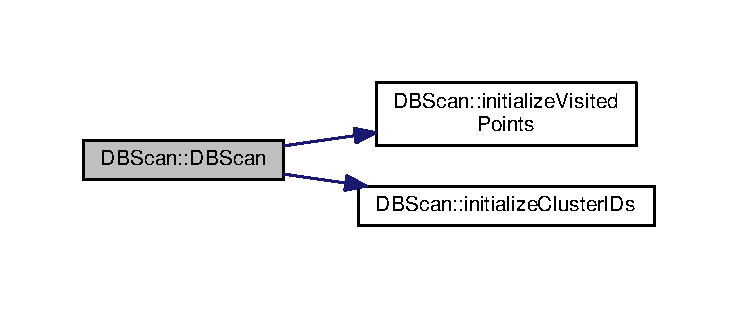
\includegraphics[width=350pt]{classDBScan_adbbf078f15acf6fae053d8c288b2e97b_cgraph}
\end{center}
\end{figure}




\subsection{Member Function Documentation}
\hypertarget{classDBScan_a55a2c6e7364f2780b2032182d3616bde}{\index{D\-B\-Scan@{D\-B\-Scan}!alg\-D\-B\-Scan\-Parallel@{alg\-D\-B\-Scan\-Parallel}}
\index{alg\-D\-B\-Scan\-Parallel@{alg\-D\-B\-Scan\-Parallel}!DBScan@{D\-B\-Scan}}
\subsubsection[{alg\-D\-B\-Scan\-Parallel}]{\setlength{\rightskip}{0pt plus 5cm}void D\-B\-Scan\-::alg\-D\-B\-Scan\-Parallel (
\begin{DoxyParamCaption}
{}
\end{DoxyParamCaption}
)}}\label{classDBScan_a55a2c6e7364f2780b2032182d3616bde}
Allows clustering in parallel of multiple variants Uses a single R-\/tree index, but separate buffers for each thread 

Here is the call graph for this function\-:\nopagebreak
\begin{figure}[H]
\begin{center}
\leavevmode
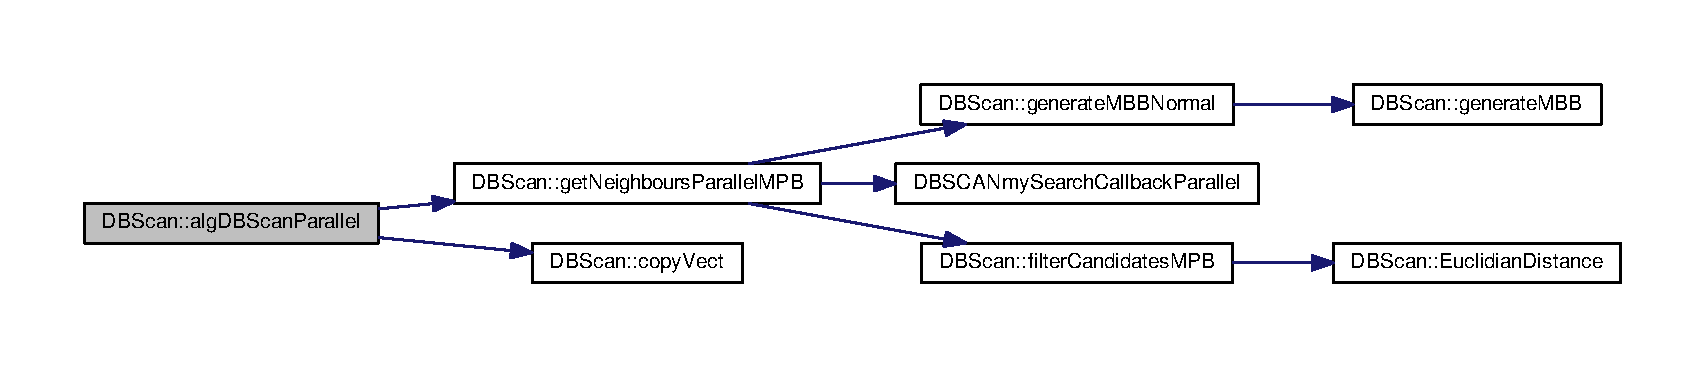
\includegraphics[width=350pt]{classDBScan_a55a2c6e7364f2780b2032182d3616bde_cgraph}
\end{center}
\end{figure}


\hypertarget{classDBScan_a7b7115631994fa281c1dca261973e6a5}{\index{D\-B\-Scan@{D\-B\-Scan}!alg\-D\-B\-Scan\-Parallel\-Reuse\-Cluster\-Results@{alg\-D\-B\-Scan\-Parallel\-Reuse\-Cluster\-Results}}
\index{alg\-D\-B\-Scan\-Parallel\-Reuse\-Cluster\-Results@{alg\-D\-B\-Scan\-Parallel\-Reuse\-Cluster\-Results}!DBScan@{D\-B\-Scan}}
\subsubsection[{alg\-D\-B\-Scan\-Parallel\-Reuse\-Cluster\-Results}]{\setlength{\rightskip}{0pt plus 5cm}void D\-B\-Scan\-::alg\-D\-B\-Scan\-Parallel\-Reuse\-Cluster\-Results (
\begin{DoxyParamCaption}
{}
\end{DoxyParamCaption}
)}}\label{classDBScan_a7b7115631994fa281c1dca261973e6a5}
D\-B\-S\-C\-A\-N version that takes the clustered output from one instance and then reuses it for another instance 

Here is the call graph for this function\-:\nopagebreak
\begin{figure}[H]
\begin{center}
\leavevmode
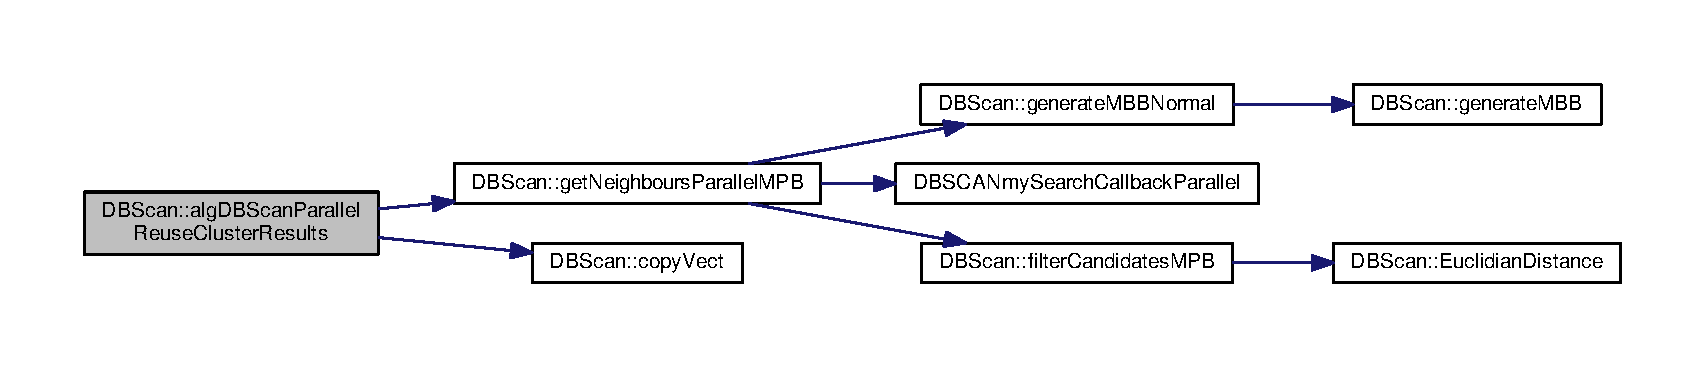
\includegraphics[width=350pt]{classDBScan_a7b7115631994fa281c1dca261973e6a5_cgraph}
\end{center}
\end{figure}


\hypertarget{classDBScan_a25383a5401de748f1525cd1aa3705afb}{\index{D\-B\-Scan@{D\-B\-Scan}!append\-M\-B\-B\-By\-Epsilon@{append\-M\-B\-B\-By\-Epsilon}}
\index{append\-M\-B\-B\-By\-Epsilon@{append\-M\-B\-B\-By\-Epsilon}!DBScan@{D\-B\-Scan}}
\subsubsection[{append\-M\-B\-B\-By\-Epsilon}]{\setlength{\rightskip}{0pt plus 5cm}void D\-B\-Scan\-::append\-M\-B\-B\-By\-Epsilon (
\begin{DoxyParamCaption}
\item[{double $\ast$}]{M\-B\-B\-\_\-min, }
\item[{double $\ast$}]{M\-B\-B\-\_\-max, }
\item[{double}]{eps}
\end{DoxyParamCaption}
)}}\label{classDBScan_a25383a5401de748f1525cd1aa3705afb}
Method that appends an M\-B\-B by epsilon \hypertarget{classDBScan_a31e46e492a6b4a6baa6682f8faf0e2de}{\index{D\-B\-Scan@{D\-B\-Scan}!assign\-Points\-To\-Predefined\-Cluster@{assign\-Points\-To\-Predefined\-Cluster}}
\index{assign\-Points\-To\-Predefined\-Cluster@{assign\-Points\-To\-Predefined\-Cluster}!DBScan@{D\-B\-Scan}}
\subsubsection[{assign\-Points\-To\-Predefined\-Cluster}]{\setlength{\rightskip}{0pt plus 5cm}void D\-B\-Scan\-::assign\-Points\-To\-Predefined\-Cluster (
\begin{DoxyParamCaption}
\item[{int}]{finished\-Instance\-I\-D}
\end{DoxyParamCaption}
)}}\label{classDBScan_a31e46e492a6b4a6baa6682f8faf0e2de}
Method that builds new clusters from previously generated clusters 

Here is the call graph for this function\-:\nopagebreak
\begin{figure}[H]
\begin{center}
\leavevmode
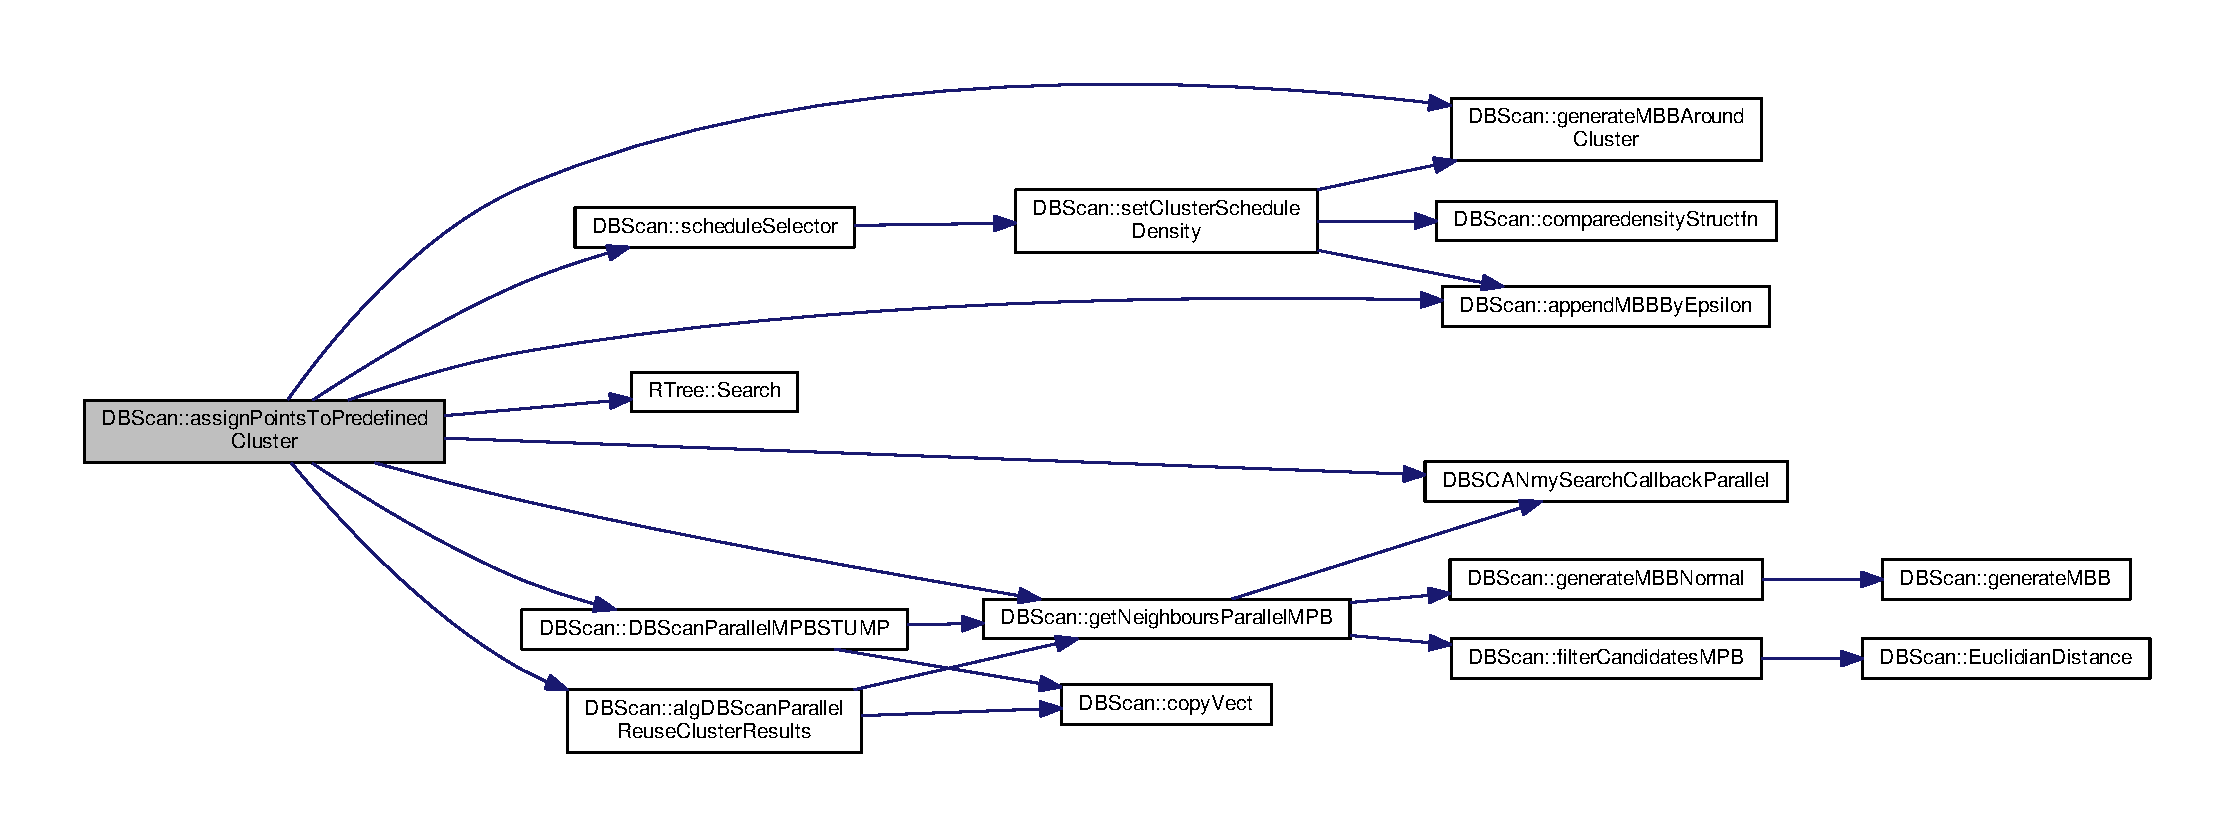
\includegraphics[width=350pt]{classDBScan_a31e46e492a6b4a6baa6682f8faf0e2de_cgraph}
\end{center}
\end{figure}


\hypertarget{classDBScan_abf662378982ad01ee4b4b0e713887d42}{\index{D\-B\-Scan@{D\-B\-Scan}!comparedensity\-Structfn@{comparedensity\-Structfn}}
\index{comparedensity\-Structfn@{comparedensity\-Structfn}!DBScan@{D\-B\-Scan}}
\subsubsection[{comparedensity\-Structfn}]{\setlength{\rightskip}{0pt plus 5cm}bool D\-B\-Scan\-::comparedensity\-Structfn (
\begin{DoxyParamCaption}
\item[{const {\bf density\-Struct} \&}]{a, }
\item[{const {\bf density\-Struct} \&}]{b}
\end{DoxyParamCaption}
)\hspace{0.3cm}{\ttfamily [static]}}}\label{classDBScan_abf662378982ad01ee4b4b0e713887d42}
Comparison function \hypertarget{classDBScan_af954708e115d00319a5cb53faffd52b1}{\index{D\-B\-Scan@{D\-B\-Scan}!copy\-Vect@{copy\-Vect}}
\index{copy\-Vect@{copy\-Vect}!DBScan@{D\-B\-Scan}}
\subsubsection[{copy\-Vect}]{\setlength{\rightskip}{0pt plus 5cm}void D\-B\-Scan\-::copy\-Vect (
\begin{DoxyParamCaption}
\item[{std\-::vector$<$ int $>$ $\ast$}]{dest, }
\item[{std\-::vector$<$ int $>$ $\ast$}]{source}
\end{DoxyParamCaption}
)\hspace{0.3cm}{\ttfamily [private]}}}\label{classDBScan_af954708e115d00319a5cb53faffd52b1}
copies the contents from the source vector and appends them to the dest vector \hypertarget{classDBScan_abaad1d98678fbf99b1c6c67fc3474a3f}{\index{D\-B\-Scan@{D\-B\-Scan}!D\-B\-Scan\-Parallel\-M\-P\-B\-S\-T\-U\-M\-P@{D\-B\-Scan\-Parallel\-M\-P\-B\-S\-T\-U\-M\-P}}
\index{D\-B\-Scan\-Parallel\-M\-P\-B\-S\-T\-U\-M\-P@{D\-B\-Scan\-Parallel\-M\-P\-B\-S\-T\-U\-M\-P}!DBScan@{D\-B\-Scan}}
\subsubsection[{D\-B\-Scan\-Parallel\-M\-P\-B\-S\-T\-U\-M\-P}]{\setlength{\rightskip}{0pt plus 5cm}void D\-B\-Scan\-::\-D\-B\-Scan\-Parallel\-M\-P\-B\-S\-T\-U\-M\-P (
\begin{DoxyParamCaption}
\item[{int}]{finished\-Instance\-I\-D, }
\item[{bool $\ast$}]{destroyed\-Arr, }
\item[{std\-::vector$<$ int $>$ $\ast$}]{candidates\-To\-Grow\-From}
\end{DoxyParamCaption}
)}}\label{classDBScan_abaad1d98678fbf99b1c6c67fc3474a3f}
\char`\"{}\-Stump\char`\"{} of \hyperlink{classDBScan}{D\-B\-Scan} used when assigning points to predefined clusters just the part of the algorithm that expands the eps-\/neighbourhood 

Here is the call graph for this function\-:\nopagebreak
\begin{figure}[H]
\begin{center}
\leavevmode
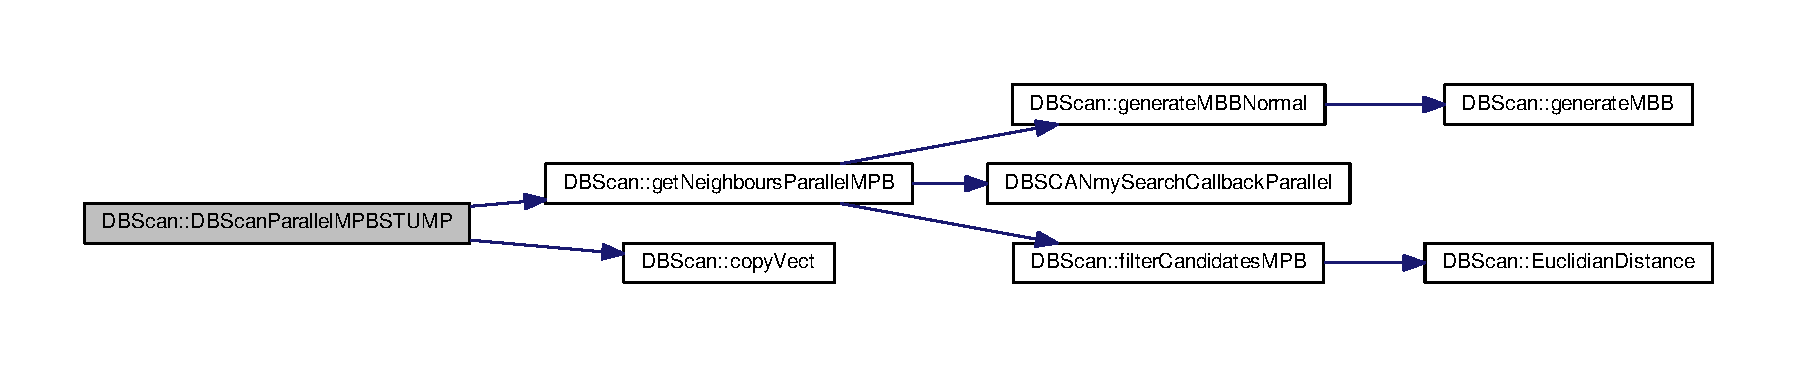
\includegraphics[width=350pt]{classDBScan_abaad1d98678fbf99b1c6c67fc3474a3f_cgraph}
\end{center}
\end{figure}


\hypertarget{classDBScan_ab42218899ad9b1f5b432df5a3c0c82d3}{\index{D\-B\-Scan@{D\-B\-Scan}!Euclidian\-Distance@{Euclidian\-Distance}}
\index{Euclidian\-Distance@{Euclidian\-Distance}!DBScan@{D\-B\-Scan}}
\subsubsection[{Euclidian\-Distance}]{\setlength{\rightskip}{0pt plus 5cm}double D\-B\-Scan\-::\-Euclidian\-Distance (
\begin{DoxyParamCaption}
\item[{struct {\bf data\-Elem} $\ast$}]{point1, }
\item[{struct {\bf data\-Elem} $\ast$}]{point2}
\end{DoxyParamCaption}
)\hspace{0.3cm}{\ttfamily [private]}}}\label{classDBScan_ab42218899ad9b1f5b432df5a3c0c82d3}
Euclidian distance calculation between two points to filter the candidate set \hypertarget{classDBScan_a62ea9b65ded887ede6d8b675aef2ce17}{\index{D\-B\-Scan@{D\-B\-Scan}!filter\-Candidates\-M\-P\-B@{filter\-Candidates\-M\-P\-B}}
\index{filter\-Candidates\-M\-P\-B@{filter\-Candidates\-M\-P\-B}!DBScan@{D\-B\-Scan}}
\subsubsection[{filter\-Candidates\-M\-P\-B}]{\setlength{\rightskip}{0pt plus 5cm}int D\-B\-Scan\-::filter\-Candidates\-M\-P\-B (
\begin{DoxyParamCaption}
\item[{struct {\bf data\-Elem} $\ast$}]{point, }
\item[{std\-::vector$<$ int $>$ $\ast$}]{candidate\-Set, }
\item[{double}]{distance, }
\item[{std\-::vector$<$ int $>$ $\ast$}]{set\-I\-Ds\-In\-Dist\-Ptr}
\end{DoxyParamCaption}
)\hspace{0.3cm}{\ttfamily [private]}}}\label{classDBScan_a62ea9b65ded887ede6d8b675aef2ce17}
Filter candidate points from the index search 

Here is the call graph for this function\-:\nopagebreak
\begin{figure}[H]
\begin{center}
\leavevmode
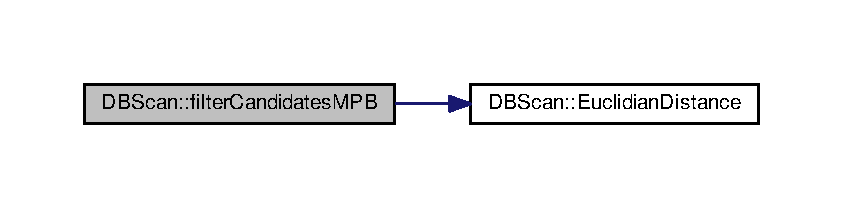
\includegraphics[width=350pt]{classDBScan_a62ea9b65ded887ede6d8b675aef2ce17_cgraph}
\end{center}
\end{figure}


\hypertarget{classDBScan_ae133eef10ed34bf676d46b1dee6af918}{\index{D\-B\-Scan@{D\-B\-Scan}!generate\-M\-B\-B@{generate\-M\-B\-B}}
\index{generate\-M\-B\-B@{generate\-M\-B\-B}!DBScan@{D\-B\-Scan}}
\subsubsection[{generate\-M\-B\-B}]{\setlength{\rightskip}{0pt plus 5cm}void D\-B\-Scan\-::generate\-M\-B\-B (
\begin{DoxyParamCaption}
\item[{struct {\bf data\-Elem} $\ast$}]{point, }
\item[{double}]{distance, }
\item[{double $\ast$}]{M\-B\-B\-\_\-min, }
\item[{double $\ast$}]{M\-B\-B\-\_\-max}
\end{DoxyParamCaption}
)\hspace{0.3cm}{\ttfamily [private]}}}\label{classDBScan_ae133eef10ed34bf676d46b1dee6af918}
M\-B\-B generation. The \char`\"{}\-Normal\char`\"{} refers to when we had the periodic boundary condition for the datasets and we did not need to wrap around generate a query M\-B\-B around the point to search for the values \hypertarget{classDBScan_a7d85d5c3c8c06c22dd4c77769baf8104}{\index{D\-B\-Scan@{D\-B\-Scan}!generate\-M\-B\-B\-Around\-Cluster@{generate\-M\-B\-B\-Around\-Cluster}}
\index{generate\-M\-B\-B\-Around\-Cluster@{generate\-M\-B\-B\-Around\-Cluster}!DBScan@{D\-B\-Scan}}
\subsubsection[{generate\-M\-B\-B\-Around\-Cluster}]{\setlength{\rightskip}{0pt plus 5cm}void D\-B\-Scan\-::generate\-M\-B\-B\-Around\-Cluster (
\begin{DoxyParamCaption}
\item[{std\-::vector$<$ int $>$ $\ast$}]{cluster\-Points, }
\item[{double $\ast$}]{M\-B\-B\-\_\-min, }
\item[{double $\ast$}]{M\-B\-B\-\_\-max}
\end{DoxyParamCaption}
)}}\label{classDBScan_a7d85d5c3c8c06c22dd4c77769baf8104}
Method that generates an M\-B\-B around a cluster for reusing data between variants \hypertarget{classDBScan_a8d882d909001edadc803668743908cc9}{\index{D\-B\-Scan@{D\-B\-Scan}!generate\-M\-B\-B\-Normal@{generate\-M\-B\-B\-Normal}}
\index{generate\-M\-B\-B\-Normal@{generate\-M\-B\-B\-Normal}!DBScan@{D\-B\-Scan}}
\subsubsection[{generate\-M\-B\-B\-Normal}]{\setlength{\rightskip}{0pt plus 5cm}bool D\-B\-Scan\-::generate\-M\-B\-B\-Normal (
\begin{DoxyParamCaption}
\item[{struct {\bf data\-Elem} $\ast$}]{point, }
\item[{double}]{distance, }
\item[{double $\ast$}]{M\-B\-B\-\_\-min, }
\item[{double $\ast$}]{M\-B\-B\-\_\-max}
\end{DoxyParamCaption}
)\hspace{0.3cm}{\ttfamily [private]}}}\label{classDBScan_a8d882d909001edadc803668743908cc9}
M\-B\-B generation. The \char`\"{}\-Normal\char`\"{} refers to when we had the periodic boundary condition for the datasets and we did not need to wrap around generate a query M\-B\-B around the point to search for the values 

Here is the call graph for this function\-:\nopagebreak
\begin{figure}[H]
\begin{center}
\leavevmode
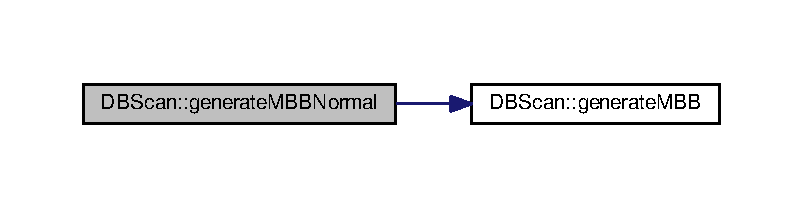
\includegraphics[width=350pt]{classDBScan_a8d882d909001edadc803668743908cc9_cgraph}
\end{center}
\end{figure}


\hypertarget{classDBScan_ab9f99900ed37f14a166d9c9cc486101a}{\index{D\-B\-Scan@{D\-B\-Scan}!get\-D\-B\-Scan\-Num\-Clusters@{get\-D\-B\-Scan\-Num\-Clusters}}
\index{get\-D\-B\-Scan\-Num\-Clusters@{get\-D\-B\-Scan\-Num\-Clusters}!DBScan@{D\-B\-Scan}}
\subsubsection[{get\-D\-B\-Scan\-Num\-Clusters}]{\setlength{\rightskip}{0pt plus 5cm}int D\-B\-Scan\-::get\-D\-B\-Scan\-Num\-Clusters (
\begin{DoxyParamCaption}
{}
\end{DoxyParamCaption}
)}}\label{classDBScan_ab9f99900ed37f14a166d9c9cc486101a}
Gets the number of clusters generated by a \hyperlink{classDBScan}{D\-B\-Scan} instance for reusing data \hypertarget{classDBScan_ab8c34378017cfa3238a08986ba273522}{\index{D\-B\-Scan@{D\-B\-Scan}!get\-Neighbours\-Parallel\-M\-P\-B@{get\-Neighbours\-Parallel\-M\-P\-B}}
\index{get\-Neighbours\-Parallel\-M\-P\-B@{get\-Neighbours\-Parallel\-M\-P\-B}!DBScan@{D\-B\-Scan}}
\subsubsection[{get\-Neighbours\-Parallel\-M\-P\-B}]{\setlength{\rightskip}{0pt plus 5cm}void D\-B\-Scan\-::get\-Neighbours\-Parallel\-M\-P\-B (
\begin{DoxyParamCaption}
\item[{struct {\bf data\-Elem} $\ast$}]{point, }
\item[{double}]{distance, }
\item[{std\-::vector$<$ int $>$ $\ast$}]{set\-I\-Ds\-In\-Dist\-Ptr}
\end{DoxyParamCaption}
)\hspace{0.3cm}{\ttfamily [private]}}}\label{classDBScan_ab8c34378017cfa3238a08986ba273522}
Epsilon-\/neighborhood search 

Here is the call graph for this function\-:\nopagebreak
\begin{figure}[H]
\begin{center}
\leavevmode
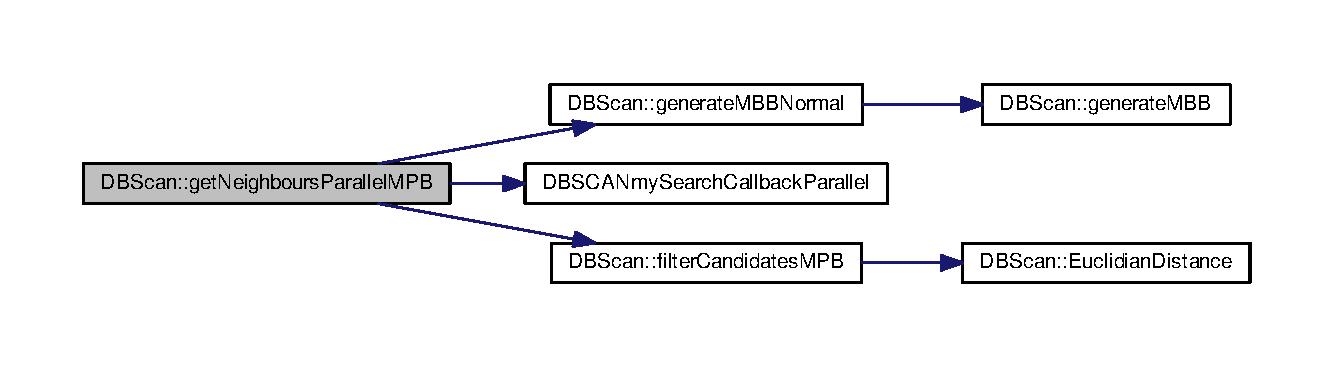
\includegraphics[width=350pt]{classDBScan_ab8c34378017cfa3238a08986ba273522_cgraph}
\end{center}
\end{figure}


\hypertarget{classDBScan_acb4f0c75d09349200c0a354033d32e6c}{\index{D\-B\-Scan@{D\-B\-Scan}!initialize\-Cluster\-I\-Ds@{initialize\-Cluster\-I\-Ds}}
\index{initialize\-Cluster\-I\-Ds@{initialize\-Cluster\-I\-Ds}!DBScan@{D\-B\-Scan}}
\subsubsection[{initialize\-Cluster\-I\-Ds}]{\setlength{\rightskip}{0pt plus 5cm}void D\-B\-Scan\-::initialize\-Cluster\-I\-Ds (
\begin{DoxyParamCaption}
\item[{int}]{size}
\end{DoxyParamCaption}
)\hspace{0.3cm}{\ttfamily [private]}}}\label{classDBScan_acb4f0c75d09349200c0a354033d32e6c}
initializes the vector storing the I\-Ds of the cluster of the data points \hypertarget{classDBScan_ab919d93ea8f7c4ef59d5112b05ec109b}{\index{D\-B\-Scan@{D\-B\-Scan}!initialize\-Visited\-Points@{initialize\-Visited\-Points}}
\index{initialize\-Visited\-Points@{initialize\-Visited\-Points}!DBScan@{D\-B\-Scan}}
\subsubsection[{initialize\-Visited\-Points}]{\setlength{\rightskip}{0pt plus 5cm}void D\-B\-Scan\-::initialize\-Visited\-Points (
\begin{DoxyParamCaption}
\item[{int}]{size}
\end{DoxyParamCaption}
)\hspace{0.3cm}{\ttfamily [private]}}}\label{classDBScan_ab919d93ea8f7c4ef59d5112b05ec109b}
initialize all of the points to initially not be visited \hypertarget{classDBScan_ab6eb34d3cad064c121cc156920e62270}{\index{D\-B\-Scan@{D\-B\-Scan}!schedule\-Selector@{schedule\-Selector}}
\index{schedule\-Selector@{schedule\-Selector}!DBScan@{D\-B\-Scan}}
\subsubsection[{schedule\-Selector}]{\setlength{\rightskip}{0pt plus 5cm}void D\-B\-Scan\-::schedule\-Selector (
\begin{DoxyParamCaption}
\item[{std\-::vector$<$ int $>$ $\ast$}]{schedule, }
\item[{std\-::vector$<$ int $>$}]{cluster\-Arr\mbox{[}$\,$\mbox{]}, }
\item[{int}]{num\-Clusters\-In\-Other\-Instance}
\end{DoxyParamCaption}
)}}\label{classDBScan_ab6eb34d3cad064c121cc156920e62270}
Selects the cluster reuse criteria Clus\-Density in the paper only 

Here is the call graph for this function\-:\nopagebreak
\begin{figure}[H]
\begin{center}
\leavevmode
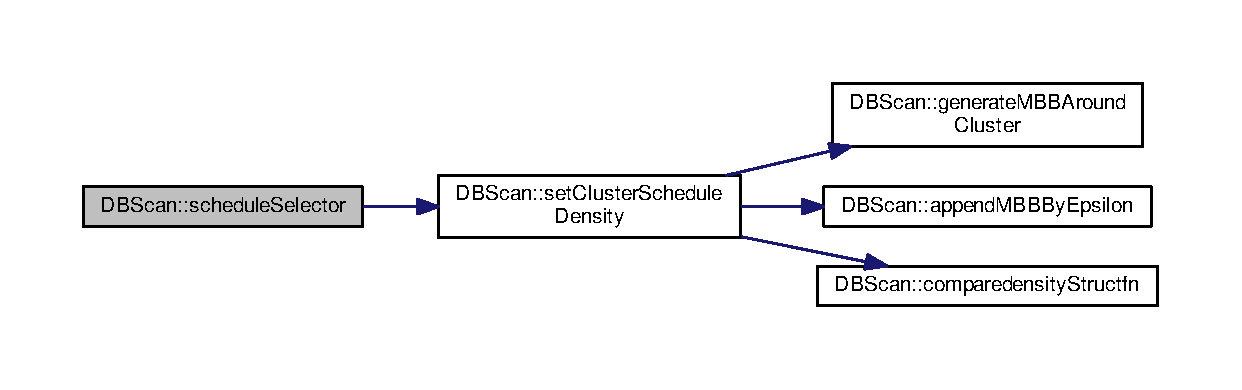
\includegraphics[width=350pt]{classDBScan_ab6eb34d3cad064c121cc156920e62270_cgraph}
\end{center}
\end{figure}


\hypertarget{classDBScan_a186a8a9666a4b66bd002e8bf568b0747}{\index{D\-B\-Scan@{D\-B\-Scan}!set\-Cluster\-Schedule\-Density@{set\-Cluster\-Schedule\-Density}}
\index{set\-Cluster\-Schedule\-Density@{set\-Cluster\-Schedule\-Density}!DBScan@{D\-B\-Scan}}
\subsubsection[{set\-Cluster\-Schedule\-Density}]{\setlength{\rightskip}{0pt plus 5cm}void D\-B\-Scan\-::set\-Cluster\-Schedule\-Density (
\begin{DoxyParamCaption}
\item[{std\-::vector$<$ int $>$ $\ast$}]{schedule, }
\item[{std\-::vector$<$ int $>$}]{cluster\-Arr\mbox{[}$\,$\mbox{]}, }
\item[{int}]{num\-Clusters\-In\-Other\-Instance}
\end{DoxyParamCaption}
)}}\label{classDBScan_a186a8a9666a4b66bd002e8bf568b0747}
\hyperlink{classSchedule}{Schedule} of cluster reuse processing based on density (Clus\-Density in the paper) 

Here is the call graph for this function\-:\nopagebreak
\begin{figure}[H]
\begin{center}
\leavevmode
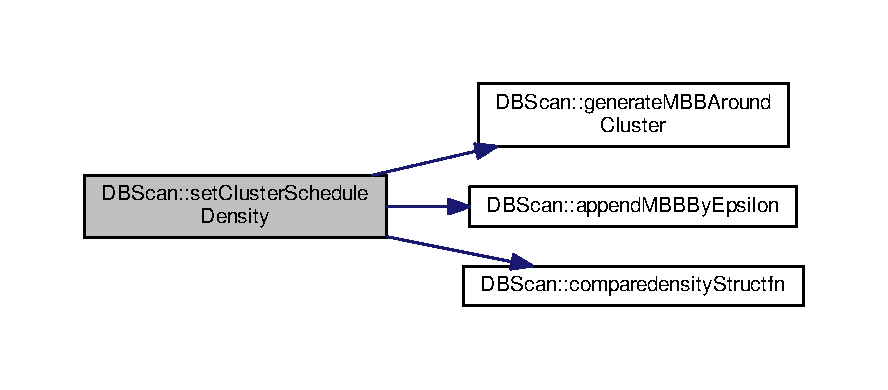
\includegraphics[width=350pt]{classDBScan_a186a8a9666a4b66bd002e8bf568b0747_cgraph}
\end{center}
\end{figure}




\subsection{Field Documentation}
\hypertarget{classDBScan_af88f51ce2f50e9f26c813426131497e9}{\index{D\-B\-Scan@{D\-B\-Scan}!cluster\-Cnt@{cluster\-Cnt}}
\index{cluster\-Cnt@{cluster\-Cnt}!DBScan@{D\-B\-Scan}}
\subsubsection[{cluster\-Cnt}]{\setlength{\rightskip}{0pt plus 5cm}int D\-B\-Scan\-::cluster\-Cnt\hspace{0.3cm}{\ttfamily [private]}}}\label{classDBScan_af88f51ce2f50e9f26c813426131497e9}
the number of clusters found after calling the algorithm \hypertarget{classDBScan_aa363c8aa510fcbd54979f16047d5f0a3}{\index{D\-B\-Scan@{D\-B\-Scan}!cluster\-I\-Ds@{cluster\-I\-Ds}}
\index{cluster\-I\-Ds@{cluster\-I\-Ds}!DBScan@{D\-B\-Scan}}
\subsubsection[{cluster\-I\-Ds}]{\setlength{\rightskip}{0pt plus 5cm}std\-::vector$<$int$>$ D\-B\-Scan\-::cluster\-I\-Ds}}\label{classDBScan_aa363c8aa510fcbd54979f16047d5f0a3}
Vector that keeps track of the assignment of the points to a cluster. Cluster 0 means a noise point. The indices of the vector correspond to the data points. Element i in cluster\-I\-Ds corresponds to the cluster that data element i is in within the data\-Points struct. \hypertarget{classDBScan_a247c7a0e0cd8f2aa24770bced14b82b5}{\index{D\-B\-Scan@{D\-B\-Scan}!data\-Points@{data\-Points}}
\index{data\-Points@{data\-Points}!DBScan@{D\-B\-Scan}}
\subsubsection[{data\-Points}]{\setlength{\rightskip}{0pt plus 5cm}std\-::vector$<$struct {\bf data\-Elem}$>$$\ast$ D\-B\-Scan\-::data\-Points\hspace{0.3cm}{\ttfamily [private]}}}\label{classDBScan_a247c7a0e0cd8f2aa24770bced14b82b5}
pointer to the data elements \hypertarget{classDBScan_a9878125297973f29db8b41287e0c9b4d}{\index{D\-B\-Scan@{D\-B\-Scan}!distance@{distance}}
\index{distance@{distance}!DBScan@{D\-B\-Scan}}
\subsubsection[{distance}]{\setlength{\rightskip}{0pt plus 5cm}double D\-B\-Scan\-::distance\hspace{0.3cm}{\ttfamily [private]}}}\label{classDBScan_a9878125297973f29db8b41287e0c9b4d}
D\-B\-S\-C\-A\-N Epsilon parameter \hypertarget{classDBScan_a8270fd572c31089b33fff1e047c00633}{\index{D\-B\-Scan@{D\-B\-Scan}!instance\-Vect@{instance\-Vect}}
\index{instance\-Vect@{instance\-Vect}!DBScan@{D\-B\-Scan}}
\subsubsection[{instance\-Vect}]{\setlength{\rightskip}{0pt plus 5cm}std\-::vector$<${\bf D\-B\-Scan} $\ast$$>$ D\-B\-Scan\-::instance\-Vect}}\label{classDBScan_a8270fd572c31089b33fff1e047c00633}
Vector of pointers to the \hyperlink{classDBScan}{D\-B\-Scan} instances that may have points for data reuse \hypertarget{classDBScan_ad117fc93029bcc699b919bb17e658292}{\index{D\-B\-Scan@{D\-B\-Scan}!min\-Pts@{min\-Pts}}
\index{min\-Pts@{min\-Pts}!DBScan@{D\-B\-Scan}}
\subsubsection[{min\-Pts}]{\setlength{\rightskip}{0pt plus 5cm}int D\-B\-Scan\-::min\-Pts\hspace{0.3cm}{\ttfamily [private]}}}\label{classDBScan_ad117fc93029bcc699b919bb17e658292}
D\-B\-S\-C\-A\-N Min\-Pts parameter \hypertarget{classDBScan_abf8ba9bc0c2b8ff8fab4c9d070f78ec7}{\index{D\-B\-Scan@{D\-B\-Scan}!num\-Clusters\-For\-Stats@{num\-Clusters\-For\-Stats}}
\index{num\-Clusters\-For\-Stats@{num\-Clusters\-For\-Stats}!DBScan@{D\-B\-Scan}}
\subsubsection[{num\-Clusters\-For\-Stats}]{\setlength{\rightskip}{0pt plus 5cm}int D\-B\-Scan\-::num\-Clusters\-For\-Stats}}\label{classDBScan_abf8ba9bc0c2b8ff8fab4c9d070f78ec7}
The number of clusters created (for statistics) \hypertarget{classDBScan_a4f4c2b033e9c3ec3bfb1cc43744e36a3}{\index{D\-B\-Scan@{D\-B\-Scan}!ptr\-M\-P\-Blookup@{ptr\-M\-P\-Blookup}}
\index{ptr\-M\-P\-Blookup@{ptr\-M\-P\-Blookup}!DBScan@{D\-B\-Scan}}
\subsubsection[{ptr\-M\-P\-Blookup}]{\setlength{\rightskip}{0pt plus 5cm}std\-::vector$<$std\-::vector$<$int$>$ $>$$\ast$ D\-B\-Scan\-::ptr\-M\-P\-Blookup\hspace{0.3cm}{\ttfamily [private]}}}\label{classDBScan_a4f4c2b033e9c3ec3bfb1cc43744e36a3}
pointer to the lookup array for multiple pointers per M\-B\-B (M\-P\-B) \hypertarget{classDBScan_affdefd0416bc3ba42ee2c069d8ac7eb3}{\index{D\-B\-Scan@{D\-B\-Scan}!set\-I\-Ds\-In\-Dist@{set\-I\-Ds\-In\-Dist}}
\index{set\-I\-Ds\-In\-Dist@{set\-I\-Ds\-In\-Dist}!DBScan@{D\-B\-Scan}}
\subsubsection[{set\-I\-Ds\-In\-Dist}]{\setlength{\rightskip}{0pt plus 5cm}std\-::vector$<$int$>$ D\-B\-Scan\-::set\-I\-Ds\-In\-Dist\hspace{0.3cm}{\ttfamily [private]}}}\label{classDBScan_affdefd0416bc3ba42ee2c069d8ac7eb3}
temporary vector used to store the ids of the candidates that are actually within the threshold distance \hypertarget{classDBScan_a406fc451a7b6b25b11cb08545a03e281}{\index{D\-B\-Scan@{D\-B\-Scan}!tree@{tree}}
\index{tree@{tree}!DBScan@{D\-B\-Scan}}
\subsubsection[{tree}]{\setlength{\rightskip}{0pt plus 5cm}{\bf R\-Tree}$<$int,double,2,float$>$$\ast$ D\-B\-Scan\-::tree\hspace{0.3cm}{\ttfamily [private]}}}\label{classDBScan_a406fc451a7b6b25b11cb08545a03e281}
pointer to the R-\/tree index \hypertarget{classDBScan_a8fd30e735fa3b426e519a8ecb7586c4d}{\index{D\-B\-Scan@{D\-B\-Scan}!tree\-High\-Resolution@{tree\-High\-Resolution}}
\index{tree\-High\-Resolution@{tree\-High\-Resolution}!DBScan@{D\-B\-Scan}}
\subsubsection[{tree\-High\-Resolution}]{\setlength{\rightskip}{0pt plus 5cm}{\bf R\-Tree}$<$int,double,2,float$>$$\ast$ D\-B\-Scan\-::tree\-High\-Resolution\hspace{0.3cm}{\ttfamily [private]}}}\label{classDBScan_a8fd30e735fa3b426e519a8ecb7586c4d}
pointer to the R-\/tree index that has 1 point per box when results can be reused across clustering runs \hypertarget{classDBScan_a03bbe4567af4354c0cba4e580cf72578}{\index{D\-B\-Scan@{D\-B\-Scan}!visited@{visited}}
\index{visited@{visited}!DBScan@{D\-B\-Scan}}
\subsubsection[{visited}]{\setlength{\rightskip}{0pt plus 5cm}std\-::vector$<$bool$>$ D\-B\-Scan\-::visited\hspace{0.3cm}{\ttfamily [private]}}}\label{classDBScan_a03bbe4567af4354c0cba4e580cf72578}
vector that keeps track of the points that have beeen visited 

The documentation for this class was generated from the following files\-:\begin{DoxyCompactItemize}
\item 
\hyperlink{DBScan_8h}{D\-B\-Scan.\-h}\item 
\hyperlink{DBScan_8cpp}{D\-B\-Scan.\-cpp}\end{DoxyCompactItemize}

\hypertarget{structdensityStruct}{\section{density\-Struct Struct Reference}
\label{structdensityStruct}\index{density\-Struct@{density\-Struct}}
}


{\ttfamily \#include \char`\"{}structs.\-h\char`\"{}}

\subsection*{Data Fields}
\begin{DoxyCompactItemize}
\item 
int \hyperlink{structdensityStruct_a7c209b566dfbfd5a064658f685b9a03b}{cluster\-I\-D}
\item 
double \hyperlink{structdensityStruct_a573f3fc839f723b35b89c0e553b1e14d}{density}
\end{DoxyCompactItemize}


\subsection{Detailed Description}
Struct used to order the clusters that will get reused 

\subsection{Field Documentation}
\hypertarget{structdensityStruct_a7c209b566dfbfd5a064658f685b9a03b}{\index{density\-Struct@{density\-Struct}!cluster\-I\-D@{cluster\-I\-D}}
\index{cluster\-I\-D@{cluster\-I\-D}!densityStruct@{density\-Struct}}
\subsubsection[{cluster\-I\-D}]{\setlength{\rightskip}{0pt plus 5cm}int density\-Struct\-::cluster\-I\-D}}\label{structdensityStruct_a7c209b566dfbfd5a064658f685b9a03b}
\hypertarget{structdensityStruct_a573f3fc839f723b35b89c0e553b1e14d}{\index{density\-Struct@{density\-Struct}!density@{density}}
\index{density@{density}!densityStruct@{density\-Struct}}
\subsubsection[{density}]{\setlength{\rightskip}{0pt plus 5cm}double density\-Struct\-::density}}\label{structdensityStruct_a573f3fc839f723b35b89c0e553b1e14d}


The documentation for this struct was generated from the following file\-:\begin{DoxyCompactItemize}
\item 
\hyperlink{structs_8h}{structs.\-h}\end{DoxyCompactItemize}

\hypertarget{structexperiment}{\section{experiment Struct Reference}
\label{structexperiment}\index{experiment@{experiment}}
}


{\ttfamily \#include \char`\"{}structs.\-h\char`\"{}}

\subsection*{Data Fields}
\begin{DoxyCompactItemize}
\item 
double \hyperlink{structexperiment_a70602e57b3b76374d22d13d09676c6b9}{epsilon}
\item 
int \hyperlink{structexperiment_aec1a30392753fcec1d80ff38a8153abf}{minpts}
\item 
unsigned int \hyperlink{structexperiment_ad062e46649cd40a782750159d0ce0d05}{variant\-I\-D}
\end{DoxyCompactItemize}


\subsection{Detailed Description}
Struct that outlines the parameters for multiple instances of \hyperlink{classDBScan}{D\-B\-Scan}, each one described per struct. 

\subsection{Field Documentation}
\hypertarget{structexperiment_a70602e57b3b76374d22d13d09676c6b9}{\index{experiment@{experiment}!epsilon@{epsilon}}
\index{epsilon@{epsilon}!experiment@{experiment}}
\subsubsection[{epsilon}]{\setlength{\rightskip}{0pt plus 5cm}double experiment\-::epsilon}}\label{structexperiment_a70602e57b3b76374d22d13d09676c6b9}
\hypertarget{structexperiment_aec1a30392753fcec1d80ff38a8153abf}{\index{experiment@{experiment}!minpts@{minpts}}
\index{minpts@{minpts}!experiment@{experiment}}
\subsubsection[{minpts}]{\setlength{\rightskip}{0pt plus 5cm}int experiment\-::minpts}}\label{structexperiment_aec1a30392753fcec1d80ff38a8153abf}
\hypertarget{structexperiment_ad062e46649cd40a782750159d0ce0d05}{\index{experiment@{experiment}!variant\-I\-D@{variant\-I\-D}}
\index{variant\-I\-D@{variant\-I\-D}!experiment@{experiment}}
\subsubsection[{variant\-I\-D}]{\setlength{\rightskip}{0pt plus 5cm}unsigned int experiment\-::variant\-I\-D}}\label{structexperiment_ad062e46649cd40a782750159d0ce0d05}


The documentation for this struct was generated from the following file\-:\begin{DoxyCompactItemize}
\item 
\hyperlink{structs_8h}{structs.\-h}\end{DoxyCompactItemize}

\hypertarget{classRTree_1_1Iterator}{\section{R\-Tree$<$ D\-A\-T\-A\-T\-Y\-P\-E, E\-L\-E\-M\-T\-Y\-P\-E, N\-U\-M\-D\-I\-M\-S, E\-L\-E\-M\-T\-Y\-P\-E\-R\-E\-A\-L, T\-M\-A\-X\-N\-O\-D\-E\-S, T\-M\-I\-N\-N\-O\-D\-E\-S $>$\-:\-:Iterator Class Reference}
\label{classRTree_1_1Iterator}\index{R\-Tree$<$ D\-A\-T\-A\-T\-Y\-P\-E, E\-L\-E\-M\-T\-Y\-P\-E, N\-U\-M\-D\-I\-M\-S, E\-L\-E\-M\-T\-Y\-P\-E\-R\-E\-A\-L, T\-M\-A\-X\-N\-O\-D\-E\-S, T\-M\-I\-N\-N\-O\-D\-E\-S $>$\-::\-Iterator@{R\-Tree$<$ D\-A\-T\-A\-T\-Y\-P\-E, E\-L\-E\-M\-T\-Y\-P\-E, N\-U\-M\-D\-I\-M\-S, E\-L\-E\-M\-T\-Y\-P\-E\-R\-E\-A\-L, T\-M\-A\-X\-N\-O\-D\-E\-S, T\-M\-I\-N\-N\-O\-D\-E\-S $>$\-::\-Iterator}}
}


\hyperlink{classRTree_1_1Iterator}{Iterator} is not remove safe.  




{\ttfamily \#include \char`\"{}R\-Tree.\-h\char`\"{}}



Collaboration diagram for R\-Tree$<$ D\-A\-T\-A\-T\-Y\-P\-E, E\-L\-E\-M\-T\-Y\-P\-E, N\-U\-M\-D\-I\-M\-S, E\-L\-E\-M\-T\-Y\-P\-E\-R\-E\-A\-L, T\-M\-A\-X\-N\-O\-D\-E\-S, T\-M\-I\-N\-N\-O\-D\-E\-S $>$\-:\-:Iterator\-:\nopagebreak
\begin{figure}[H]
\begin{center}
\leavevmode
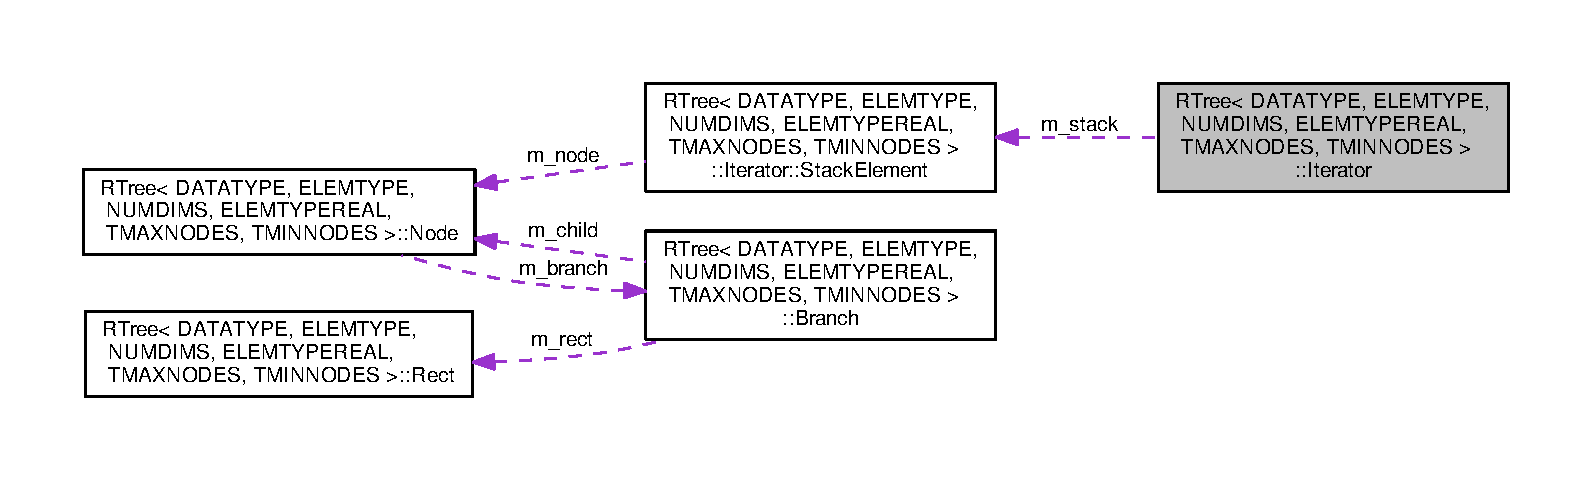
\includegraphics[width=350pt]{classRTree_1_1Iterator__coll__graph}
\end{center}
\end{figure}
\subsection*{Data Structures}
\begin{DoxyCompactItemize}
\item 
struct \hyperlink{structRTree_1_1Iterator_1_1StackElement}{Stack\-Element}
\end{DoxyCompactItemize}
\subsection*{Public Member Functions}
\begin{DoxyCompactItemize}
\item 
\hyperlink{classRTree_1_1Iterator_a59b2600d21bebdbfd5406ae42612ef7f}{Iterator} ()
\item 
\hyperlink{classRTree_1_1Iterator_a4823daecb48994f28175139ccbd763d8}{$\sim$\-Iterator} ()
\item 
bool \hyperlink{classRTree_1_1Iterator_a23f756ac37acc2b162b61230c27732b3}{Is\-Null} ()
\begin{DoxyCompactList}\small\item\em Is iterator invalid. \end{DoxyCompactList}\item 
bool \hyperlink{classRTree_1_1Iterator_a8cd6bf4fa228497ac736e8d7993e7daf}{Is\-Not\-Null} ()
\begin{DoxyCompactList}\small\item\em Is iterator pointing to valid data. \end{DoxyCompactList}\item 
D\-A\-T\-A\-T\-Y\-P\-E \& \hyperlink{classRTree_1_1Iterator_abb61d3a8396473b543cb15aa9002cfeb}{operator$\ast$} ()
\begin{DoxyCompactList}\small\item\em Access the current data element. Caller must be sure iterator is not N\-U\-L\-L first. \end{DoxyCompactList}\item 
const D\-A\-T\-A\-T\-Y\-P\-E \& \hyperlink{classRTree_1_1Iterator_a45496ad72eba6929d40239ed711bf129}{operator$\ast$} () const 
\begin{DoxyCompactList}\small\item\em Access the current data element. Caller must be sure iterator is not N\-U\-L\-L first. \end{DoxyCompactList}\item 
bool \hyperlink{classRTree_1_1Iterator_ad578bac71cfc7d324b84595032feda21}{operator++} ()
\begin{DoxyCompactList}\small\item\em Find the next data element. \end{DoxyCompactList}\item 
void \hyperlink{classRTree_1_1Iterator_abbf4f08d825f6b475b7cdb6e5bc223d7}{Get\-Data} (D\-A\-T\-A\-T\-Y\-P\-E $\ast$t\-\_\-id, D\-A\-T\-A\-T\-Y\-P\-E $\ast$t\-\_\-segment\-\_\-id)
\item 
void \hyperlink{classRTree_1_1Iterator_a65121f5016c2b1bf4696797748092709}{Get\-Bounds} (E\-L\-E\-M\-T\-Y\-P\-E a\-\_\-min\mbox{[}N\-U\-M\-D\-I\-M\-S\mbox{]}, E\-L\-E\-M\-T\-Y\-P\-E a\-\_\-max\mbox{[}N\-U\-M\-D\-I\-M\-S\mbox{]})
\begin{DoxyCompactList}\small\item\em Get the bounds for this node. \end{DoxyCompactList}\end{DoxyCompactItemize}
\subsection*{Private Types}
\begin{DoxyCompactItemize}
\item 
enum \{ \hyperlink{classRTree_1_1Iterator_a1e45c4c1d6d735b999df1cbe1a0e36ada26b6ad9c0a591145b71370b87ce125e8}{M\-A\-X\-\_\-\-S\-T\-A\-C\-K} = 32
 \}
\end{DoxyCompactItemize}
\subsection*{Private Member Functions}
\begin{DoxyCompactItemize}
\item 
void \hyperlink{classRTree_1_1Iterator_a923e4fe7dc813630c4b20b8468f9dcc7}{Init} ()
\begin{DoxyCompactList}\small\item\em Reset iterator. \end{DoxyCompactList}\item 
bool \hyperlink{classRTree_1_1Iterator_ae1dc5968481efa8c8c916323472b159b}{Find\-Next\-Data} ()
\begin{DoxyCompactList}\small\item\em Find the next data element in the tree (For internal use only) \end{DoxyCompactList}\item 
void \hyperlink{classRTree_1_1Iterator_afb35dcd6c652052684d5e8801d9cda7c}{Push} (\hyperlink{structRTree_1_1Node}{Node} $\ast$a\-\_\-node, int a\-\_\-branch\-Index)
\begin{DoxyCompactList}\small\item\em Push node and branch onto iteration stack (For internal use only) \end{DoxyCompactList}\item 
\hyperlink{structRTree_1_1Iterator_1_1StackElement}{Stack\-Element} \& \hyperlink{classRTree_1_1Iterator_a6f75eaf8c9ebe60f4a8cacbb7f4998fe}{Pop} ()
\begin{DoxyCompactList}\small\item\em Pop element off iteration stack (For internal use only) \end{DoxyCompactList}\end{DoxyCompactItemize}
\subsection*{Private Attributes}
\begin{DoxyCompactItemize}
\item 
\hyperlink{structRTree_1_1Iterator_1_1StackElement}{Stack\-Element} \hyperlink{classRTree_1_1Iterator_a71a0c70b553212a62c135343831f74b0}{m\-\_\-stack} \mbox{[}\hyperlink{classRTree_1_1Iterator_a1e45c4c1d6d735b999df1cbe1a0e36ada26b6ad9c0a591145b71370b87ce125e8}{M\-A\-X\-\_\-\-S\-T\-A\-C\-K}\mbox{]}
\begin{DoxyCompactList}\small\item\em Stack as we are doing iteration instead of recursion. \end{DoxyCompactList}\item 
int \hyperlink{classRTree_1_1Iterator_aa925698d64e938a5644b4ccdb247fd97}{m\-\_\-tos}
\begin{DoxyCompactList}\small\item\em Top Of Stack index. \end{DoxyCompactList}\end{DoxyCompactItemize}
\subsection*{Friends}
\begin{DoxyCompactItemize}
\item 
class \hyperlink{classRTree_1_1Iterator_af5d7fbb9e949ef77e8d3e32670fa9dd6}{R\-Tree}
\end{DoxyCompactItemize}


\subsection{Detailed Description}
\subsubsection*{template$<$class D\-A\-T\-A\-T\-Y\-P\-E, class E\-L\-E\-M\-T\-Y\-P\-E, int N\-U\-M\-D\-I\-M\-S, class E\-L\-E\-M\-T\-Y\-P\-E\-R\-E\-A\-L = E\-L\-E\-M\-T\-Y\-P\-E, int T\-M\-A\-X\-N\-O\-D\-E\-S = 8, int T\-M\-I\-N\-N\-O\-D\-E\-S = T\-M\-A\-X\-N\-O\-D\-E\-S / 2$>$class R\-Tree$<$ D\-A\-T\-A\-T\-Y\-P\-E, E\-L\-E\-M\-T\-Y\-P\-E, N\-U\-M\-D\-I\-M\-S, E\-L\-E\-M\-T\-Y\-P\-E\-R\-E\-A\-L, T\-M\-A\-X\-N\-O\-D\-E\-S, T\-M\-I\-N\-N\-O\-D\-E\-S $>$\-::\-Iterator}

\hyperlink{classRTree_1_1Iterator}{Iterator} is not remove safe. 

\subsection{Member Enumeration Documentation}
\hypertarget{classRTree_1_1Iterator_a1e45c4c1d6d735b999df1cbe1a0e36ad}{\subsubsection[{anonymous enum}]{\setlength{\rightskip}{0pt plus 5cm}template$<$class D\-A\-T\-A\-T\-Y\-P\-E, class E\-L\-E\-M\-T\-Y\-P\-E, int N\-U\-M\-D\-I\-M\-S, class E\-L\-E\-M\-T\-Y\-P\-E\-R\-E\-A\-L = E\-L\-E\-M\-T\-Y\-P\-E, int T\-M\-A\-X\-N\-O\-D\-E\-S = 8, int T\-M\-I\-N\-N\-O\-D\-E\-S = T\-M\-A\-X\-N\-O\-D\-E\-S / 2$>$ anonymous enum\hspace{0.3cm}{\ttfamily [private]}}}\label{classRTree_1_1Iterator_a1e45c4c1d6d735b999df1cbe1a0e36ad}
\begin{Desc}
\item[Enumerator]\par
\begin{description}
\index{M\-A\-X\-\_\-\-S\-T\-A\-C\-K@{M\-A\-X\-\_\-\-S\-T\-A\-C\-K}!R\-Tree\-::\-Iterator@{R\-Tree\-::\-Iterator}}\index{R\-Tree\-::\-Iterator@{R\-Tree\-::\-Iterator}!M\-A\-X\-\_\-\-S\-T\-A\-C\-K@{M\-A\-X\-\_\-\-S\-T\-A\-C\-K}}\item[{\em 
\hypertarget{classRTree_1_1Iterator_a1e45c4c1d6d735b999df1cbe1a0e36ada26b6ad9c0a591145b71370b87ce125e8}{M\-A\-X\-\_\-\-S\-T\-A\-C\-K}\label{classRTree_1_1Iterator_a1e45c4c1d6d735b999df1cbe1a0e36ada26b6ad9c0a591145b71370b87ce125e8}
}]\end{description}
\end{Desc}


\subsection{Constructor \& Destructor Documentation}
\hypertarget{classRTree_1_1Iterator_a59b2600d21bebdbfd5406ae42612ef7f}{\index{R\-Tree\-::\-Iterator@{R\-Tree\-::\-Iterator}!Iterator@{Iterator}}
\index{Iterator@{Iterator}!RTree::Iterator@{R\-Tree\-::\-Iterator}}
\subsubsection[{Iterator}]{\setlength{\rightskip}{0pt plus 5cm}template$<$class D\-A\-T\-A\-T\-Y\-P\-E, class E\-L\-E\-M\-T\-Y\-P\-E, int N\-U\-M\-D\-I\-M\-S, class E\-L\-E\-M\-T\-Y\-P\-E\-R\-E\-A\-L = E\-L\-E\-M\-T\-Y\-P\-E, int T\-M\-A\-X\-N\-O\-D\-E\-S = 8, int T\-M\-I\-N\-N\-O\-D\-E\-S = T\-M\-A\-X\-N\-O\-D\-E\-S / 2$>$ {\bf R\-Tree}$<$ D\-A\-T\-A\-T\-Y\-P\-E, E\-L\-E\-M\-T\-Y\-P\-E, N\-U\-M\-D\-I\-M\-S, E\-L\-E\-M\-T\-Y\-P\-E\-R\-E\-A\-L, T\-M\-A\-X\-N\-O\-D\-E\-S, T\-M\-I\-N\-N\-O\-D\-E\-S $>$\-::Iterator\-::\-Iterator (
\begin{DoxyParamCaption}
{}
\end{DoxyParamCaption}
)\hspace{0.3cm}{\ttfamily [inline]}}}\label{classRTree_1_1Iterator_a59b2600d21bebdbfd5406ae42612ef7f}


Here is the call graph for this function\-:\nopagebreak
\begin{figure}[H]
\begin{center}
\leavevmode
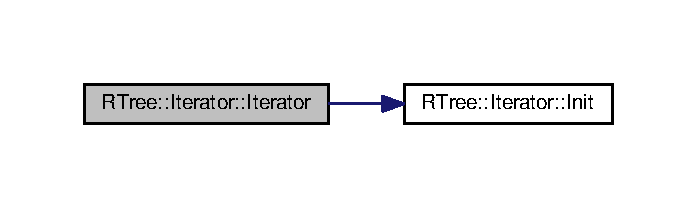
\includegraphics[width=334pt]{classRTree_1_1Iterator_a59b2600d21bebdbfd5406ae42612ef7f_cgraph}
\end{center}
\end{figure}


\hypertarget{classRTree_1_1Iterator_a4823daecb48994f28175139ccbd763d8}{\index{R\-Tree\-::\-Iterator@{R\-Tree\-::\-Iterator}!$\sim$\-Iterator@{$\sim$\-Iterator}}
\index{$\sim$\-Iterator@{$\sim$\-Iterator}!RTree::Iterator@{R\-Tree\-::\-Iterator}}
\subsubsection[{$\sim$\-Iterator}]{\setlength{\rightskip}{0pt plus 5cm}template$<$class D\-A\-T\-A\-T\-Y\-P\-E, class E\-L\-E\-M\-T\-Y\-P\-E, int N\-U\-M\-D\-I\-M\-S, class E\-L\-E\-M\-T\-Y\-P\-E\-R\-E\-A\-L = E\-L\-E\-M\-T\-Y\-P\-E, int T\-M\-A\-X\-N\-O\-D\-E\-S = 8, int T\-M\-I\-N\-N\-O\-D\-E\-S = T\-M\-A\-X\-N\-O\-D\-E\-S / 2$>$ {\bf R\-Tree}$<$ D\-A\-T\-A\-T\-Y\-P\-E, E\-L\-E\-M\-T\-Y\-P\-E, N\-U\-M\-D\-I\-M\-S, E\-L\-E\-M\-T\-Y\-P\-E\-R\-E\-A\-L, T\-M\-A\-X\-N\-O\-D\-E\-S, T\-M\-I\-N\-N\-O\-D\-E\-S $>$\-::Iterator\-::$\sim$\-Iterator (
\begin{DoxyParamCaption}
{}
\end{DoxyParamCaption}
)\hspace{0.3cm}{\ttfamily [inline]}}}\label{classRTree_1_1Iterator_a4823daecb48994f28175139ccbd763d8}


\subsection{Member Function Documentation}
\hypertarget{classRTree_1_1Iterator_ae1dc5968481efa8c8c916323472b159b}{\index{R\-Tree\-::\-Iterator@{R\-Tree\-::\-Iterator}!Find\-Next\-Data@{Find\-Next\-Data}}
\index{Find\-Next\-Data@{Find\-Next\-Data}!RTree::Iterator@{R\-Tree\-::\-Iterator}}
\subsubsection[{Find\-Next\-Data}]{\setlength{\rightskip}{0pt plus 5cm}template$<$class D\-A\-T\-A\-T\-Y\-P\-E, class E\-L\-E\-M\-T\-Y\-P\-E, int N\-U\-M\-D\-I\-M\-S, class E\-L\-E\-M\-T\-Y\-P\-E\-R\-E\-A\-L = E\-L\-E\-M\-T\-Y\-P\-E, int T\-M\-A\-X\-N\-O\-D\-E\-S = 8, int T\-M\-I\-N\-N\-O\-D\-E\-S = T\-M\-A\-X\-N\-O\-D\-E\-S / 2$>$ bool {\bf R\-Tree}$<$ D\-A\-T\-A\-T\-Y\-P\-E, E\-L\-E\-M\-T\-Y\-P\-E, N\-U\-M\-D\-I\-M\-S, E\-L\-E\-M\-T\-Y\-P\-E\-R\-E\-A\-L, T\-M\-A\-X\-N\-O\-D\-E\-S, T\-M\-I\-N\-N\-O\-D\-E\-S $>$\-::Iterator\-::\-Find\-Next\-Data (
\begin{DoxyParamCaption}
{}
\end{DoxyParamCaption}
)\hspace{0.3cm}{\ttfamily [inline]}, {\ttfamily [private]}}}\label{classRTree_1_1Iterator_ae1dc5968481efa8c8c916323472b159b}


Find the next data element in the tree (For internal use only) 



Here is the call graph for this function\-:\nopagebreak
\begin{figure}[H]
\begin{center}
\leavevmode
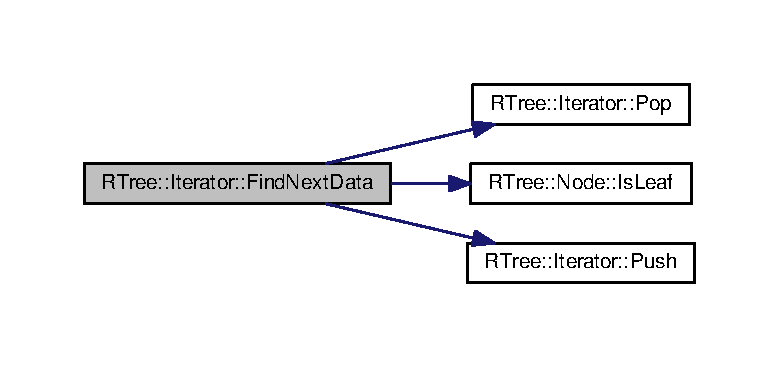
\includegraphics[width=350pt]{classRTree_1_1Iterator_ae1dc5968481efa8c8c916323472b159b_cgraph}
\end{center}
\end{figure}


\hypertarget{classRTree_1_1Iterator_a65121f5016c2b1bf4696797748092709}{\index{R\-Tree\-::\-Iterator@{R\-Tree\-::\-Iterator}!Get\-Bounds@{Get\-Bounds}}
\index{Get\-Bounds@{Get\-Bounds}!RTree::Iterator@{R\-Tree\-::\-Iterator}}
\subsubsection[{Get\-Bounds}]{\setlength{\rightskip}{0pt plus 5cm}template$<$class D\-A\-T\-A\-T\-Y\-P\-E, class E\-L\-E\-M\-T\-Y\-P\-E, int N\-U\-M\-D\-I\-M\-S, class E\-L\-E\-M\-T\-Y\-P\-E\-R\-E\-A\-L = E\-L\-E\-M\-T\-Y\-P\-E, int T\-M\-A\-X\-N\-O\-D\-E\-S = 8, int T\-M\-I\-N\-N\-O\-D\-E\-S = T\-M\-A\-X\-N\-O\-D\-E\-S / 2$>$ void {\bf R\-Tree}$<$ D\-A\-T\-A\-T\-Y\-P\-E, E\-L\-E\-M\-T\-Y\-P\-E, N\-U\-M\-D\-I\-M\-S, E\-L\-E\-M\-T\-Y\-P\-E\-R\-E\-A\-L, T\-M\-A\-X\-N\-O\-D\-E\-S, T\-M\-I\-N\-N\-O\-D\-E\-S $>$\-::Iterator\-::\-Get\-Bounds (
\begin{DoxyParamCaption}
\item[{E\-L\-E\-M\-T\-Y\-P\-E}]{a\-\_\-min\mbox{[}\-N\-U\-M\-D\-I\-M\-S\mbox{]}, }
\item[{E\-L\-E\-M\-T\-Y\-P\-E}]{a\-\_\-max\mbox{[}\-N\-U\-M\-D\-I\-M\-S\mbox{]}}
\end{DoxyParamCaption}
)\hspace{0.3cm}{\ttfamily [inline]}}}\label{classRTree_1_1Iterator_a65121f5016c2b1bf4696797748092709}


Get the bounds for this node. 



Here is the call graph for this function\-:\nopagebreak
\begin{figure}[H]
\begin{center}
\leavevmode
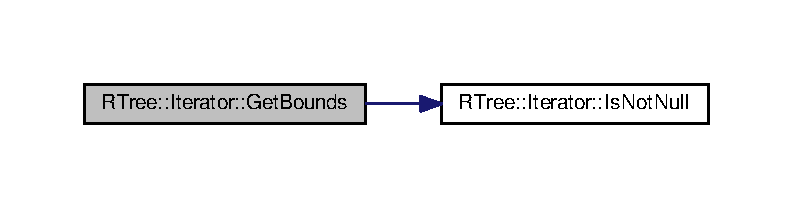
\includegraphics[width=350pt]{classRTree_1_1Iterator_a65121f5016c2b1bf4696797748092709_cgraph}
\end{center}
\end{figure}


\hypertarget{classRTree_1_1Iterator_abbf4f08d825f6b475b7cdb6e5bc223d7}{\index{R\-Tree\-::\-Iterator@{R\-Tree\-::\-Iterator}!Get\-Data@{Get\-Data}}
\index{Get\-Data@{Get\-Data}!RTree::Iterator@{R\-Tree\-::\-Iterator}}
\subsubsection[{Get\-Data}]{\setlength{\rightskip}{0pt plus 5cm}template$<$class D\-A\-T\-A\-T\-Y\-P\-E, class E\-L\-E\-M\-T\-Y\-P\-E, int N\-U\-M\-D\-I\-M\-S, class E\-L\-E\-M\-T\-Y\-P\-E\-R\-E\-A\-L = E\-L\-E\-M\-T\-Y\-P\-E, int T\-M\-A\-X\-N\-O\-D\-E\-S = 8, int T\-M\-I\-N\-N\-O\-D\-E\-S = T\-M\-A\-X\-N\-O\-D\-E\-S / 2$>$ void {\bf R\-Tree}$<$ D\-A\-T\-A\-T\-Y\-P\-E, E\-L\-E\-M\-T\-Y\-P\-E, N\-U\-M\-D\-I\-M\-S, E\-L\-E\-M\-T\-Y\-P\-E\-R\-E\-A\-L, T\-M\-A\-X\-N\-O\-D\-E\-S, T\-M\-I\-N\-N\-O\-D\-E\-S $>$\-::Iterator\-::\-Get\-Data (
\begin{DoxyParamCaption}
\item[{D\-A\-T\-A\-T\-Y\-P\-E $\ast$}]{t\-\_\-id, }
\item[{D\-A\-T\-A\-T\-Y\-P\-E $\ast$}]{t\-\_\-segment\-\_\-id}
\end{DoxyParamCaption}
)\hspace{0.3cm}{\ttfamily [inline]}}}\label{classRTree_1_1Iterator_abbf4f08d825f6b475b7cdb6e5bc223d7}


Here is the call graph for this function\-:\nopagebreak
\begin{figure}[H]
\begin{center}
\leavevmode
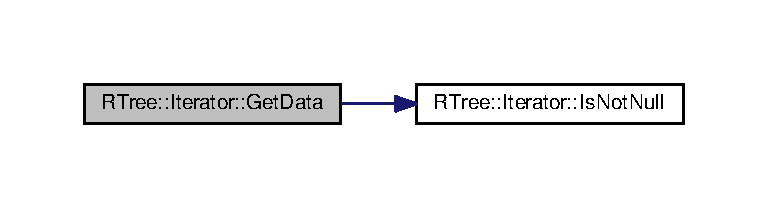
\includegraphics[width=350pt]{classRTree_1_1Iterator_abbf4f08d825f6b475b7cdb6e5bc223d7_cgraph}
\end{center}
\end{figure}


\hypertarget{classRTree_1_1Iterator_a923e4fe7dc813630c4b20b8468f9dcc7}{\index{R\-Tree\-::\-Iterator@{R\-Tree\-::\-Iterator}!Init@{Init}}
\index{Init@{Init}!RTree::Iterator@{R\-Tree\-::\-Iterator}}
\subsubsection[{Init}]{\setlength{\rightskip}{0pt plus 5cm}template$<$class D\-A\-T\-A\-T\-Y\-P\-E, class E\-L\-E\-M\-T\-Y\-P\-E, int N\-U\-M\-D\-I\-M\-S, class E\-L\-E\-M\-T\-Y\-P\-E\-R\-E\-A\-L = E\-L\-E\-M\-T\-Y\-P\-E, int T\-M\-A\-X\-N\-O\-D\-E\-S = 8, int T\-M\-I\-N\-N\-O\-D\-E\-S = T\-M\-A\-X\-N\-O\-D\-E\-S / 2$>$ void {\bf R\-Tree}$<$ D\-A\-T\-A\-T\-Y\-P\-E, E\-L\-E\-M\-T\-Y\-P\-E, N\-U\-M\-D\-I\-M\-S, E\-L\-E\-M\-T\-Y\-P\-E\-R\-E\-A\-L, T\-M\-A\-X\-N\-O\-D\-E\-S, T\-M\-I\-N\-N\-O\-D\-E\-S $>$\-::Iterator\-::\-Init (
\begin{DoxyParamCaption}
{}
\end{DoxyParamCaption}
)\hspace{0.3cm}{\ttfamily [inline]}, {\ttfamily [private]}}}\label{classRTree_1_1Iterator_a923e4fe7dc813630c4b20b8468f9dcc7}


Reset iterator. 

\hypertarget{classRTree_1_1Iterator_a8cd6bf4fa228497ac736e8d7993e7daf}{\index{R\-Tree\-::\-Iterator@{R\-Tree\-::\-Iterator}!Is\-Not\-Null@{Is\-Not\-Null}}
\index{Is\-Not\-Null@{Is\-Not\-Null}!RTree::Iterator@{R\-Tree\-::\-Iterator}}
\subsubsection[{Is\-Not\-Null}]{\setlength{\rightskip}{0pt plus 5cm}template$<$class D\-A\-T\-A\-T\-Y\-P\-E, class E\-L\-E\-M\-T\-Y\-P\-E, int N\-U\-M\-D\-I\-M\-S, class E\-L\-E\-M\-T\-Y\-P\-E\-R\-E\-A\-L = E\-L\-E\-M\-T\-Y\-P\-E, int T\-M\-A\-X\-N\-O\-D\-E\-S = 8, int T\-M\-I\-N\-N\-O\-D\-E\-S = T\-M\-A\-X\-N\-O\-D\-E\-S / 2$>$ bool {\bf R\-Tree}$<$ D\-A\-T\-A\-T\-Y\-P\-E, E\-L\-E\-M\-T\-Y\-P\-E, N\-U\-M\-D\-I\-M\-S, E\-L\-E\-M\-T\-Y\-P\-E\-R\-E\-A\-L, T\-M\-A\-X\-N\-O\-D\-E\-S, T\-M\-I\-N\-N\-O\-D\-E\-S $>$\-::Iterator\-::\-Is\-Not\-Null (
\begin{DoxyParamCaption}
{}
\end{DoxyParamCaption}
)\hspace{0.3cm}{\ttfamily [inline]}}}\label{classRTree_1_1Iterator_a8cd6bf4fa228497ac736e8d7993e7daf}


Is iterator pointing to valid data. 

\hypertarget{classRTree_1_1Iterator_a23f756ac37acc2b162b61230c27732b3}{\index{R\-Tree\-::\-Iterator@{R\-Tree\-::\-Iterator}!Is\-Null@{Is\-Null}}
\index{Is\-Null@{Is\-Null}!RTree::Iterator@{R\-Tree\-::\-Iterator}}
\subsubsection[{Is\-Null}]{\setlength{\rightskip}{0pt plus 5cm}template$<$class D\-A\-T\-A\-T\-Y\-P\-E, class E\-L\-E\-M\-T\-Y\-P\-E, int N\-U\-M\-D\-I\-M\-S, class E\-L\-E\-M\-T\-Y\-P\-E\-R\-E\-A\-L = E\-L\-E\-M\-T\-Y\-P\-E, int T\-M\-A\-X\-N\-O\-D\-E\-S = 8, int T\-M\-I\-N\-N\-O\-D\-E\-S = T\-M\-A\-X\-N\-O\-D\-E\-S / 2$>$ bool {\bf R\-Tree}$<$ D\-A\-T\-A\-T\-Y\-P\-E, E\-L\-E\-M\-T\-Y\-P\-E, N\-U\-M\-D\-I\-M\-S, E\-L\-E\-M\-T\-Y\-P\-E\-R\-E\-A\-L, T\-M\-A\-X\-N\-O\-D\-E\-S, T\-M\-I\-N\-N\-O\-D\-E\-S $>$\-::Iterator\-::\-Is\-Null (
\begin{DoxyParamCaption}
{}
\end{DoxyParamCaption}
)\hspace{0.3cm}{\ttfamily [inline]}}}\label{classRTree_1_1Iterator_a23f756ac37acc2b162b61230c27732b3}


Is iterator invalid. 

\hypertarget{classRTree_1_1Iterator_abb61d3a8396473b543cb15aa9002cfeb}{\index{R\-Tree\-::\-Iterator@{R\-Tree\-::\-Iterator}!operator$\ast$@{operator$\ast$}}
\index{operator$\ast$@{operator$\ast$}!RTree::Iterator@{R\-Tree\-::\-Iterator}}
\subsubsection[{operator$\ast$}]{\setlength{\rightskip}{0pt plus 5cm}template$<$class D\-A\-T\-A\-T\-Y\-P\-E, class E\-L\-E\-M\-T\-Y\-P\-E, int N\-U\-M\-D\-I\-M\-S, class E\-L\-E\-M\-T\-Y\-P\-E\-R\-E\-A\-L = E\-L\-E\-M\-T\-Y\-P\-E, int T\-M\-A\-X\-N\-O\-D\-E\-S = 8, int T\-M\-I\-N\-N\-O\-D\-E\-S = T\-M\-A\-X\-N\-O\-D\-E\-S / 2$>$ D\-A\-T\-A\-T\-Y\-P\-E\& {\bf R\-Tree}$<$ D\-A\-T\-A\-T\-Y\-P\-E, E\-L\-E\-M\-T\-Y\-P\-E, N\-U\-M\-D\-I\-M\-S, E\-L\-E\-M\-T\-Y\-P\-E\-R\-E\-A\-L, T\-M\-A\-X\-N\-O\-D\-E\-S, T\-M\-I\-N\-N\-O\-D\-E\-S $>$\-::Iterator\-::operator$\ast$ (
\begin{DoxyParamCaption}
{}
\end{DoxyParamCaption}
)\hspace{0.3cm}{\ttfamily [inline]}}}\label{classRTree_1_1Iterator_abb61d3a8396473b543cb15aa9002cfeb}


Access the current data element. Caller must be sure iterator is not N\-U\-L\-L first. 



Here is the call graph for this function\-:\nopagebreak
\begin{figure}[H]
\begin{center}
\leavevmode
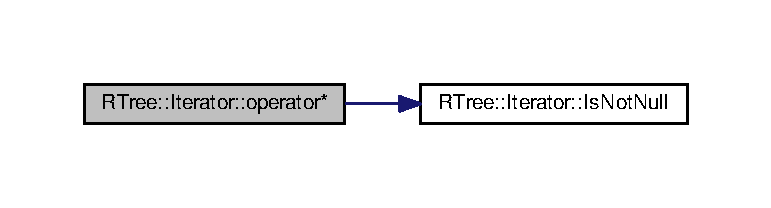
\includegraphics[width=350pt]{classRTree_1_1Iterator_abb61d3a8396473b543cb15aa9002cfeb_cgraph}
\end{center}
\end{figure}


\hypertarget{classRTree_1_1Iterator_a45496ad72eba6929d40239ed711bf129}{\index{R\-Tree\-::\-Iterator@{R\-Tree\-::\-Iterator}!operator$\ast$@{operator$\ast$}}
\index{operator$\ast$@{operator$\ast$}!RTree::Iterator@{R\-Tree\-::\-Iterator}}
\subsubsection[{operator$\ast$}]{\setlength{\rightskip}{0pt plus 5cm}template$<$class D\-A\-T\-A\-T\-Y\-P\-E, class E\-L\-E\-M\-T\-Y\-P\-E, int N\-U\-M\-D\-I\-M\-S, class E\-L\-E\-M\-T\-Y\-P\-E\-R\-E\-A\-L = E\-L\-E\-M\-T\-Y\-P\-E, int T\-M\-A\-X\-N\-O\-D\-E\-S = 8, int T\-M\-I\-N\-N\-O\-D\-E\-S = T\-M\-A\-X\-N\-O\-D\-E\-S / 2$>$ const D\-A\-T\-A\-T\-Y\-P\-E\& {\bf R\-Tree}$<$ D\-A\-T\-A\-T\-Y\-P\-E, E\-L\-E\-M\-T\-Y\-P\-E, N\-U\-M\-D\-I\-M\-S, E\-L\-E\-M\-T\-Y\-P\-E\-R\-E\-A\-L, T\-M\-A\-X\-N\-O\-D\-E\-S, T\-M\-I\-N\-N\-O\-D\-E\-S $>$\-::Iterator\-::operator$\ast$ (
\begin{DoxyParamCaption}
{}
\end{DoxyParamCaption}
) const\hspace{0.3cm}{\ttfamily [inline]}}}\label{classRTree_1_1Iterator_a45496ad72eba6929d40239ed711bf129}


Access the current data element. Caller must be sure iterator is not N\-U\-L\-L first. 



Here is the call graph for this function\-:\nopagebreak
\begin{figure}[H]
\begin{center}
\leavevmode
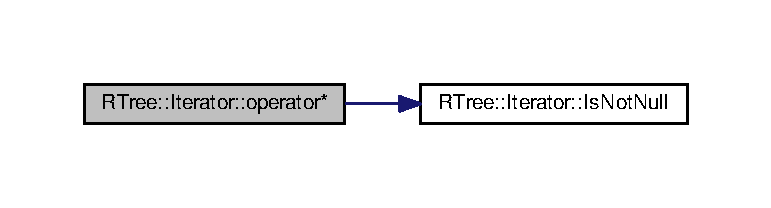
\includegraphics[width=350pt]{classRTree_1_1Iterator_a45496ad72eba6929d40239ed711bf129_cgraph}
\end{center}
\end{figure}


\hypertarget{classRTree_1_1Iterator_ad578bac71cfc7d324b84595032feda21}{\index{R\-Tree\-::\-Iterator@{R\-Tree\-::\-Iterator}!operator++@{operator++}}
\index{operator++@{operator++}!RTree::Iterator@{R\-Tree\-::\-Iterator}}
\subsubsection[{operator++}]{\setlength{\rightskip}{0pt plus 5cm}template$<$class D\-A\-T\-A\-T\-Y\-P\-E, class E\-L\-E\-M\-T\-Y\-P\-E, int N\-U\-M\-D\-I\-M\-S, class E\-L\-E\-M\-T\-Y\-P\-E\-R\-E\-A\-L = E\-L\-E\-M\-T\-Y\-P\-E, int T\-M\-A\-X\-N\-O\-D\-E\-S = 8, int T\-M\-I\-N\-N\-O\-D\-E\-S = T\-M\-A\-X\-N\-O\-D\-E\-S / 2$>$ bool {\bf R\-Tree}$<$ D\-A\-T\-A\-T\-Y\-P\-E, E\-L\-E\-M\-T\-Y\-P\-E, N\-U\-M\-D\-I\-M\-S, E\-L\-E\-M\-T\-Y\-P\-E\-R\-E\-A\-L, T\-M\-A\-X\-N\-O\-D\-E\-S, T\-M\-I\-N\-N\-O\-D\-E\-S $>$\-::Iterator\-::operator++ (
\begin{DoxyParamCaption}
{}
\end{DoxyParamCaption}
)\hspace{0.3cm}{\ttfamily [inline]}}}\label{classRTree_1_1Iterator_ad578bac71cfc7d324b84595032feda21}


Find the next data element. 



Here is the call graph for this function\-:\nopagebreak
\begin{figure}[H]
\begin{center}
\leavevmode
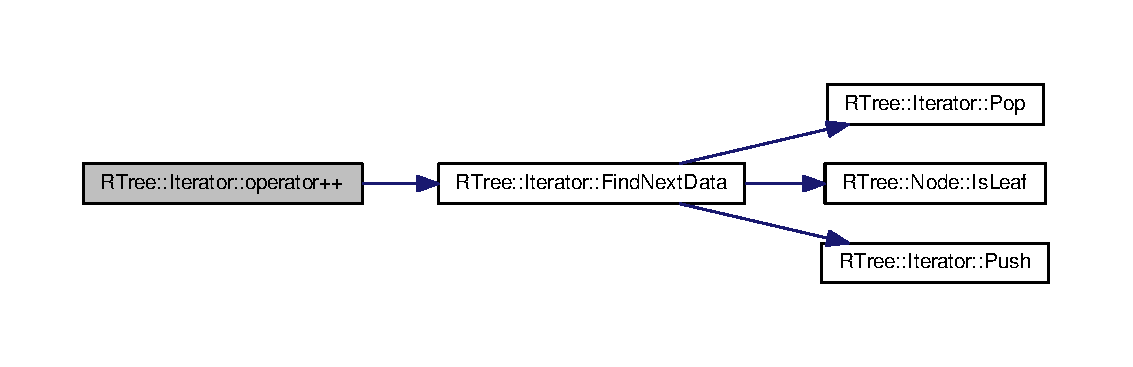
\includegraphics[width=350pt]{classRTree_1_1Iterator_ad578bac71cfc7d324b84595032feda21_cgraph}
\end{center}
\end{figure}


\hypertarget{classRTree_1_1Iterator_a6f75eaf8c9ebe60f4a8cacbb7f4998fe}{\index{R\-Tree\-::\-Iterator@{R\-Tree\-::\-Iterator}!Pop@{Pop}}
\index{Pop@{Pop}!RTree::Iterator@{R\-Tree\-::\-Iterator}}
\subsubsection[{Pop}]{\setlength{\rightskip}{0pt plus 5cm}template$<$class D\-A\-T\-A\-T\-Y\-P\-E, class E\-L\-E\-M\-T\-Y\-P\-E, int N\-U\-M\-D\-I\-M\-S, class E\-L\-E\-M\-T\-Y\-P\-E\-R\-E\-A\-L = E\-L\-E\-M\-T\-Y\-P\-E, int T\-M\-A\-X\-N\-O\-D\-E\-S = 8, int T\-M\-I\-N\-N\-O\-D\-E\-S = T\-M\-A\-X\-N\-O\-D\-E\-S / 2$>$ {\bf Stack\-Element}\& {\bf R\-Tree}$<$ D\-A\-T\-A\-T\-Y\-P\-E, E\-L\-E\-M\-T\-Y\-P\-E, N\-U\-M\-D\-I\-M\-S, E\-L\-E\-M\-T\-Y\-P\-E\-R\-E\-A\-L, T\-M\-A\-X\-N\-O\-D\-E\-S, T\-M\-I\-N\-N\-O\-D\-E\-S $>$\-::Iterator\-::\-Pop (
\begin{DoxyParamCaption}
{}
\end{DoxyParamCaption}
)\hspace{0.3cm}{\ttfamily [inline]}, {\ttfamily [private]}}}\label{classRTree_1_1Iterator_a6f75eaf8c9ebe60f4a8cacbb7f4998fe}


Pop element off iteration stack (For internal use only) 

\hypertarget{classRTree_1_1Iterator_afb35dcd6c652052684d5e8801d9cda7c}{\index{R\-Tree\-::\-Iterator@{R\-Tree\-::\-Iterator}!Push@{Push}}
\index{Push@{Push}!RTree::Iterator@{R\-Tree\-::\-Iterator}}
\subsubsection[{Push}]{\setlength{\rightskip}{0pt plus 5cm}template$<$class D\-A\-T\-A\-T\-Y\-P\-E, class E\-L\-E\-M\-T\-Y\-P\-E, int N\-U\-M\-D\-I\-M\-S, class E\-L\-E\-M\-T\-Y\-P\-E\-R\-E\-A\-L = E\-L\-E\-M\-T\-Y\-P\-E, int T\-M\-A\-X\-N\-O\-D\-E\-S = 8, int T\-M\-I\-N\-N\-O\-D\-E\-S = T\-M\-A\-X\-N\-O\-D\-E\-S / 2$>$ void {\bf R\-Tree}$<$ D\-A\-T\-A\-T\-Y\-P\-E, E\-L\-E\-M\-T\-Y\-P\-E, N\-U\-M\-D\-I\-M\-S, E\-L\-E\-M\-T\-Y\-P\-E\-R\-E\-A\-L, T\-M\-A\-X\-N\-O\-D\-E\-S, T\-M\-I\-N\-N\-O\-D\-E\-S $>$\-::Iterator\-::\-Push (
\begin{DoxyParamCaption}
\item[{{\bf Node} $\ast$}]{a\-\_\-node, }
\item[{int}]{a\-\_\-branch\-Index}
\end{DoxyParamCaption}
)\hspace{0.3cm}{\ttfamily [inline]}, {\ttfamily [private]}}}\label{classRTree_1_1Iterator_afb35dcd6c652052684d5e8801d9cda7c}


Push node and branch onto iteration stack (For internal use only) 



\subsection{Friends And Related Function Documentation}
\hypertarget{classRTree_1_1Iterator_af5d7fbb9e949ef77e8d3e32670fa9dd6}{\index{R\-Tree\-::\-Iterator@{R\-Tree\-::\-Iterator}!R\-Tree@{R\-Tree}}
\index{R\-Tree@{R\-Tree}!RTree::Iterator@{R\-Tree\-::\-Iterator}}
\subsubsection[{R\-Tree}]{\setlength{\rightskip}{0pt plus 5cm}template$<$class D\-A\-T\-A\-T\-Y\-P\-E, class E\-L\-E\-M\-T\-Y\-P\-E, int N\-U\-M\-D\-I\-M\-S, class E\-L\-E\-M\-T\-Y\-P\-E\-R\-E\-A\-L = E\-L\-E\-M\-T\-Y\-P\-E, int T\-M\-A\-X\-N\-O\-D\-E\-S = 8, int T\-M\-I\-N\-N\-O\-D\-E\-S = T\-M\-A\-X\-N\-O\-D\-E\-S / 2$>$ friend class {\bf R\-Tree}\hspace{0.3cm}{\ttfamily [friend]}}}\label{classRTree_1_1Iterator_af5d7fbb9e949ef77e8d3e32670fa9dd6}


\subsection{Field Documentation}
\hypertarget{classRTree_1_1Iterator_a71a0c70b553212a62c135343831f74b0}{\index{R\-Tree\-::\-Iterator@{R\-Tree\-::\-Iterator}!m\-\_\-stack@{m\-\_\-stack}}
\index{m\-\_\-stack@{m\-\_\-stack}!RTree::Iterator@{R\-Tree\-::\-Iterator}}
\subsubsection[{m\-\_\-stack}]{\setlength{\rightskip}{0pt plus 5cm}template$<$class D\-A\-T\-A\-T\-Y\-P\-E, class E\-L\-E\-M\-T\-Y\-P\-E, int N\-U\-M\-D\-I\-M\-S, class E\-L\-E\-M\-T\-Y\-P\-E\-R\-E\-A\-L = E\-L\-E\-M\-T\-Y\-P\-E, int T\-M\-A\-X\-N\-O\-D\-E\-S = 8, int T\-M\-I\-N\-N\-O\-D\-E\-S = T\-M\-A\-X\-N\-O\-D\-E\-S / 2$>$ {\bf Stack\-Element} {\bf R\-Tree}$<$ D\-A\-T\-A\-T\-Y\-P\-E, E\-L\-E\-M\-T\-Y\-P\-E, N\-U\-M\-D\-I\-M\-S, E\-L\-E\-M\-T\-Y\-P\-E\-R\-E\-A\-L, T\-M\-A\-X\-N\-O\-D\-E\-S, T\-M\-I\-N\-N\-O\-D\-E\-S $>$\-::Iterator\-::m\-\_\-stack\mbox{[}{\bf M\-A\-X\-\_\-\-S\-T\-A\-C\-K}\mbox{]}\hspace{0.3cm}{\ttfamily [private]}}}\label{classRTree_1_1Iterator_a71a0c70b553212a62c135343831f74b0}


Stack as we are doing iteration instead of recursion. 

\hypertarget{classRTree_1_1Iterator_aa925698d64e938a5644b4ccdb247fd97}{\index{R\-Tree\-::\-Iterator@{R\-Tree\-::\-Iterator}!m\-\_\-tos@{m\-\_\-tos}}
\index{m\-\_\-tos@{m\-\_\-tos}!RTree::Iterator@{R\-Tree\-::\-Iterator}}
\subsubsection[{m\-\_\-tos}]{\setlength{\rightskip}{0pt plus 5cm}template$<$class D\-A\-T\-A\-T\-Y\-P\-E, class E\-L\-E\-M\-T\-Y\-P\-E, int N\-U\-M\-D\-I\-M\-S, class E\-L\-E\-M\-T\-Y\-P\-E\-R\-E\-A\-L = E\-L\-E\-M\-T\-Y\-P\-E, int T\-M\-A\-X\-N\-O\-D\-E\-S = 8, int T\-M\-I\-N\-N\-O\-D\-E\-S = T\-M\-A\-X\-N\-O\-D\-E\-S / 2$>$ int {\bf R\-Tree}$<$ D\-A\-T\-A\-T\-Y\-P\-E, E\-L\-E\-M\-T\-Y\-P\-E, N\-U\-M\-D\-I\-M\-S, E\-L\-E\-M\-T\-Y\-P\-E\-R\-E\-A\-L, T\-M\-A\-X\-N\-O\-D\-E\-S, T\-M\-I\-N\-N\-O\-D\-E\-S $>$\-::Iterator\-::m\-\_\-tos\hspace{0.3cm}{\ttfamily [private]}}}\label{classRTree_1_1Iterator_aa925698d64e938a5644b4ccdb247fd97}


Top Of Stack index. 



The documentation for this class was generated from the following file\-:\begin{DoxyCompactItemize}
\item 
\hyperlink{RTree_8h}{R\-Tree.\-h}\end{DoxyCompactItemize}

\hypertarget{structRTree_1_1ListNode}{\section{R\-Tree$<$ D\-A\-T\-A\-T\-Y\-P\-E, E\-L\-E\-M\-T\-Y\-P\-E, N\-U\-M\-D\-I\-M\-S, E\-L\-E\-M\-T\-Y\-P\-E\-R\-E\-A\-L, T\-M\-A\-X\-N\-O\-D\-E\-S, T\-M\-I\-N\-N\-O\-D\-E\-S $>$\-:\-:List\-Node Struct Reference}
\label{structRTree_1_1ListNode}\index{R\-Tree$<$ D\-A\-T\-A\-T\-Y\-P\-E, E\-L\-E\-M\-T\-Y\-P\-E, N\-U\-M\-D\-I\-M\-S, E\-L\-E\-M\-T\-Y\-P\-E\-R\-E\-A\-L, T\-M\-A\-X\-N\-O\-D\-E\-S, T\-M\-I\-N\-N\-O\-D\-E\-S $>$\-::\-List\-Node@{R\-Tree$<$ D\-A\-T\-A\-T\-Y\-P\-E, E\-L\-E\-M\-T\-Y\-P\-E, N\-U\-M\-D\-I\-M\-S, E\-L\-E\-M\-T\-Y\-P\-E\-R\-E\-A\-L, T\-M\-A\-X\-N\-O\-D\-E\-S, T\-M\-I\-N\-N\-O\-D\-E\-S $>$\-::\-List\-Node}}
}


A link list of nodes for reinsertion after a delete operation.  




{\ttfamily \#include \char`\"{}R\-Tree.\-h\char`\"{}}



Collaboration diagram for R\-Tree$<$ D\-A\-T\-A\-T\-Y\-P\-E, E\-L\-E\-M\-T\-Y\-P\-E, N\-U\-M\-D\-I\-M\-S, E\-L\-E\-M\-T\-Y\-P\-E\-R\-E\-A\-L, T\-M\-A\-X\-N\-O\-D\-E\-S, T\-M\-I\-N\-N\-O\-D\-E\-S $>$\-:\-:List\-Node\-:\nopagebreak
\begin{figure}[H]
\begin{center}
\leavevmode
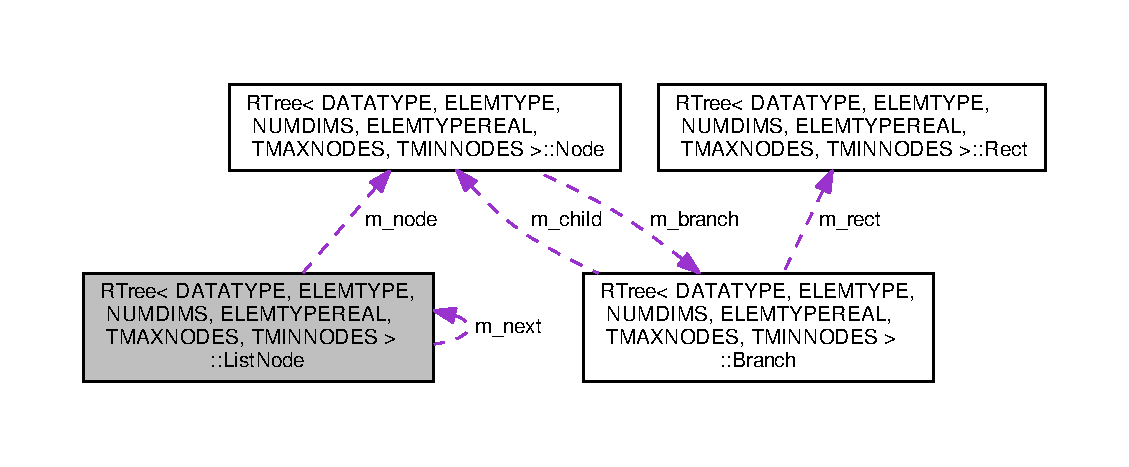
\includegraphics[width=350pt]{structRTree_1_1ListNode__coll__graph}
\end{center}
\end{figure}
\subsection*{Data Fields}
\begin{DoxyCompactItemize}
\item 
\hyperlink{structRTree_1_1ListNode}{List\-Node} $\ast$ \hyperlink{structRTree_1_1ListNode_a9812899d8953b03f1772522b668942e3}{m\-\_\-next}
\begin{DoxyCompactList}\small\item\em Next in list. \end{DoxyCompactList}\item 
\hyperlink{structRTree_1_1Node}{Node} $\ast$ \hyperlink{structRTree_1_1ListNode_ade4b7e322e04e0a71b4e14cde8e73dca}{m\-\_\-node}
\begin{DoxyCompactList}\small\item\em \hyperlink{structRTree_1_1Node}{Node}. \end{DoxyCompactList}\end{DoxyCompactItemize}


\subsection{Detailed Description}
\subsubsection*{template$<$class D\-A\-T\-A\-T\-Y\-P\-E, class E\-L\-E\-M\-T\-Y\-P\-E, int N\-U\-M\-D\-I\-M\-S, class E\-L\-E\-M\-T\-Y\-P\-E\-R\-E\-A\-L = E\-L\-E\-M\-T\-Y\-P\-E, int T\-M\-A\-X\-N\-O\-D\-E\-S = 8, int T\-M\-I\-N\-N\-O\-D\-E\-S = T\-M\-A\-X\-N\-O\-D\-E\-S / 2$>$struct R\-Tree$<$ D\-A\-T\-A\-T\-Y\-P\-E, E\-L\-E\-M\-T\-Y\-P\-E, N\-U\-M\-D\-I\-M\-S, E\-L\-E\-M\-T\-Y\-P\-E\-R\-E\-A\-L, T\-M\-A\-X\-N\-O\-D\-E\-S, T\-M\-I\-N\-N\-O\-D\-E\-S $>$\-::\-List\-Node}

A link list of nodes for reinsertion after a delete operation. 

\subsection{Field Documentation}
\hypertarget{structRTree_1_1ListNode_a9812899d8953b03f1772522b668942e3}{\index{R\-Tree\-::\-List\-Node@{R\-Tree\-::\-List\-Node}!m\-\_\-next@{m\-\_\-next}}
\index{m\-\_\-next@{m\-\_\-next}!RTree::ListNode@{R\-Tree\-::\-List\-Node}}
\subsubsection[{m\-\_\-next}]{\setlength{\rightskip}{0pt plus 5cm}template$<$class D\-A\-T\-A\-T\-Y\-P\-E, class E\-L\-E\-M\-T\-Y\-P\-E, int N\-U\-M\-D\-I\-M\-S, class E\-L\-E\-M\-T\-Y\-P\-E\-R\-E\-A\-L = E\-L\-E\-M\-T\-Y\-P\-E, int T\-M\-A\-X\-N\-O\-D\-E\-S = 8, int T\-M\-I\-N\-N\-O\-D\-E\-S = T\-M\-A\-X\-N\-O\-D\-E\-S / 2$>$ {\bf List\-Node}$\ast$ {\bf R\-Tree}$<$ D\-A\-T\-A\-T\-Y\-P\-E, E\-L\-E\-M\-T\-Y\-P\-E, N\-U\-M\-D\-I\-M\-S, E\-L\-E\-M\-T\-Y\-P\-E\-R\-E\-A\-L, T\-M\-A\-X\-N\-O\-D\-E\-S, T\-M\-I\-N\-N\-O\-D\-E\-S $>$\-::List\-Node\-::m\-\_\-next}}\label{structRTree_1_1ListNode_a9812899d8953b03f1772522b668942e3}


Next in list. 

\hypertarget{structRTree_1_1ListNode_ade4b7e322e04e0a71b4e14cde8e73dca}{\index{R\-Tree\-::\-List\-Node@{R\-Tree\-::\-List\-Node}!m\-\_\-node@{m\-\_\-node}}
\index{m\-\_\-node@{m\-\_\-node}!RTree::ListNode@{R\-Tree\-::\-List\-Node}}
\subsubsection[{m\-\_\-node}]{\setlength{\rightskip}{0pt plus 5cm}template$<$class D\-A\-T\-A\-T\-Y\-P\-E, class E\-L\-E\-M\-T\-Y\-P\-E, int N\-U\-M\-D\-I\-M\-S, class E\-L\-E\-M\-T\-Y\-P\-E\-R\-E\-A\-L = E\-L\-E\-M\-T\-Y\-P\-E, int T\-M\-A\-X\-N\-O\-D\-E\-S = 8, int T\-M\-I\-N\-N\-O\-D\-E\-S = T\-M\-A\-X\-N\-O\-D\-E\-S / 2$>$ {\bf Node}$\ast$ {\bf R\-Tree}$<$ D\-A\-T\-A\-T\-Y\-P\-E, E\-L\-E\-M\-T\-Y\-P\-E, N\-U\-M\-D\-I\-M\-S, E\-L\-E\-M\-T\-Y\-P\-E\-R\-E\-A\-L, T\-M\-A\-X\-N\-O\-D\-E\-S, T\-M\-I\-N\-N\-O\-D\-E\-S $>$\-::List\-Node\-::m\-\_\-node}}\label{structRTree_1_1ListNode_ade4b7e322e04e0a71b4e14cde8e73dca}


\hyperlink{structRTree_1_1Node}{Node}. 



The documentation for this struct was generated from the following file\-:\begin{DoxyCompactItemize}
\item 
\hyperlink{RTree_8h}{R\-Tree.\-h}\end{DoxyCompactItemize}

\hypertarget{structMPBRect}{\section{M\-P\-B\-Rect Struct Reference}
\label{structMPBRect}\index{M\-P\-B\-Rect@{M\-P\-B\-Rect}}
}


{\ttfamily \#include \char`\"{}structs.\-h\char`\"{}}

\subsection*{Public Member Functions}
\begin{DoxyCompactItemize}
\item 
void \hyperlink{structMPBRect_a033ab3752f265ead9537a7de070e074a}{Create\-M\-B\-B} (std\-::vector$<$ struct \hyperlink{structdataElem}{data\-Elem} $>$ $\ast$\hyperlink{globals_8h_ac152ac2be0eb07c2b73b4bb54a8f1952}{data\-Points}, std\-::vector$<$ int $>$ $\ast$multiple\-Points\-To\-Index)
\end{DoxyCompactItemize}
\subsection*{Data Fields}
\begin{DoxyCompactItemize}
\item 
double \hyperlink{structMPBRect_a87b98ecee53f4258063d5ba19fe04cad}{M\-B\-B\-\_\-min} \mbox{[}2\mbox{]}
\item 
double \hyperlink{structMPBRect_a1635c4ed1a66979dc1c0422a9baf7ce6}{M\-B\-B\-\_\-max} \mbox{[}2\mbox{]}
\item 
int \hyperlink{structMPBRect_a94c83296d1783e2b18c65016a0501645}{pid}
\end{DoxyCompactItemize}


\subsection{Detailed Description}
Used for the index of point objects -\/ multiple points per M\-B\-B. They make the M\-B\-Bs that are inserted into the tree (2-\/\-D M\-B\-Bs only) 

\subsection{Member Function Documentation}
\hypertarget{structMPBRect_a033ab3752f265ead9537a7de070e074a}{\index{M\-P\-B\-Rect@{M\-P\-B\-Rect}!Create\-M\-B\-B@{Create\-M\-B\-B}}
\index{Create\-M\-B\-B@{Create\-M\-B\-B}!MPBRect@{M\-P\-B\-Rect}}
\subsubsection[{Create\-M\-B\-B}]{\setlength{\rightskip}{0pt plus 5cm}void M\-P\-B\-Rect\-::\-Create\-M\-B\-B (
\begin{DoxyParamCaption}
\item[{std\-::vector$<$ struct {\bf data\-Elem} $>$ $\ast$}]{data\-Points, }
\item[{std\-::vector$<$ int $>$ $\ast$}]{multiple\-Points\-To\-Index}
\end{DoxyParamCaption}
)\hspace{0.3cm}{\ttfamily [inline]}}}\label{structMPBRect_a033ab3752f265ead9537a7de070e074a}


\subsection{Field Documentation}
\hypertarget{structMPBRect_a1635c4ed1a66979dc1c0422a9baf7ce6}{\index{M\-P\-B\-Rect@{M\-P\-B\-Rect}!M\-B\-B\-\_\-max@{M\-B\-B\-\_\-max}}
\index{M\-B\-B\-\_\-max@{M\-B\-B\-\_\-max}!MPBRect@{M\-P\-B\-Rect}}
\subsubsection[{M\-B\-B\-\_\-max}]{\setlength{\rightskip}{0pt plus 5cm}double M\-P\-B\-Rect\-::\-M\-B\-B\-\_\-max\mbox{[}2\mbox{]}}}\label{structMPBRect_a1635c4ed1a66979dc1c0422a9baf7ce6}
\hypertarget{structMPBRect_a87b98ecee53f4258063d5ba19fe04cad}{\index{M\-P\-B\-Rect@{M\-P\-B\-Rect}!M\-B\-B\-\_\-min@{M\-B\-B\-\_\-min}}
\index{M\-B\-B\-\_\-min@{M\-B\-B\-\_\-min}!MPBRect@{M\-P\-B\-Rect}}
\subsubsection[{M\-B\-B\-\_\-min}]{\setlength{\rightskip}{0pt plus 5cm}double M\-P\-B\-Rect\-::\-M\-B\-B\-\_\-min\mbox{[}2\mbox{]}}}\label{structMPBRect_a87b98ecee53f4258063d5ba19fe04cad}
\hypertarget{structMPBRect_a94c83296d1783e2b18c65016a0501645}{\index{M\-P\-B\-Rect@{M\-P\-B\-Rect}!pid@{pid}}
\index{pid@{pid}!MPBRect@{M\-P\-B\-Rect}}
\subsubsection[{pid}]{\setlength{\rightskip}{0pt plus 5cm}int M\-P\-B\-Rect\-::pid}}\label{structMPBRect_a94c83296d1783e2b18c65016a0501645}


The documentation for this struct was generated from the following file\-:\begin{DoxyCompactItemize}
\item 
\hyperlink{structs_8h}{structs.\-h}\end{DoxyCompactItemize}

\hypertarget{structRTree_1_1Node}{\section{R\-Tree$<$ D\-A\-T\-A\-T\-Y\-P\-E, E\-L\-E\-M\-T\-Y\-P\-E, N\-U\-M\-D\-I\-M\-S, E\-L\-E\-M\-T\-Y\-P\-E\-R\-E\-A\-L, T\-M\-A\-X\-N\-O\-D\-E\-S, T\-M\-I\-N\-N\-O\-D\-E\-S $>$\-:\-:Node Struct Reference}
\label{structRTree_1_1Node}\index{R\-Tree$<$ D\-A\-T\-A\-T\-Y\-P\-E, E\-L\-E\-M\-T\-Y\-P\-E, N\-U\-M\-D\-I\-M\-S, E\-L\-E\-M\-T\-Y\-P\-E\-R\-E\-A\-L, T\-M\-A\-X\-N\-O\-D\-E\-S, T\-M\-I\-N\-N\-O\-D\-E\-S $>$\-::\-Node@{R\-Tree$<$ D\-A\-T\-A\-T\-Y\-P\-E, E\-L\-E\-M\-T\-Y\-P\-E, N\-U\-M\-D\-I\-M\-S, E\-L\-E\-M\-T\-Y\-P\-E\-R\-E\-A\-L, T\-M\-A\-X\-N\-O\-D\-E\-S, T\-M\-I\-N\-N\-O\-D\-E\-S $>$\-::\-Node}}
}


\hyperlink{structRTree_1_1Node}{Node} for each branch level.  




{\ttfamily \#include \char`\"{}R\-Tree.\-h\char`\"{}}



Collaboration diagram for R\-Tree$<$ D\-A\-T\-A\-T\-Y\-P\-E, E\-L\-E\-M\-T\-Y\-P\-E, N\-U\-M\-D\-I\-M\-S, E\-L\-E\-M\-T\-Y\-P\-E\-R\-E\-A\-L, T\-M\-A\-X\-N\-O\-D\-E\-S, T\-M\-I\-N\-N\-O\-D\-E\-S $>$\-:\-:Node\-:\nopagebreak
\begin{figure}[H]
\begin{center}
\leavevmode
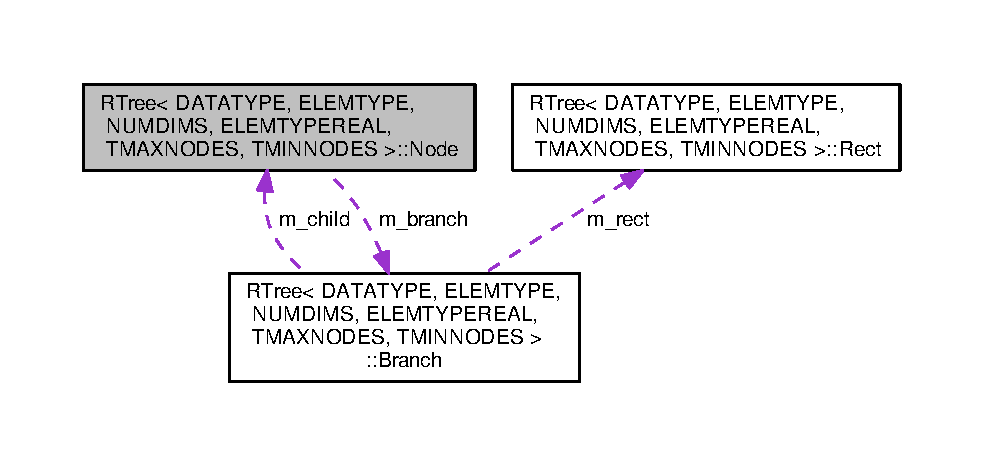
\includegraphics[width=350pt]{structRTree_1_1Node__coll__graph}
\end{center}
\end{figure}
\subsection*{Public Member Functions}
\begin{DoxyCompactItemize}
\item 
bool \hyperlink{structRTree_1_1Node_a6a330138c4d6e2280ac16770cdfcaf09}{Is\-Internal\-Node} ()
\item 
bool \hyperlink{structRTree_1_1Node_a3e34e35a8482978d456885d4bac76de4}{Is\-Leaf} ()
\end{DoxyCompactItemize}
\subsection*{Data Fields}
\begin{DoxyCompactItemize}
\item 
int \hyperlink{structRTree_1_1Node_ab2393bb1bfe7c8baa84ec4f205d990ed}{m\-\_\-count}
\begin{DoxyCompactList}\small\item\em Count. \end{DoxyCompactList}\item 
int \hyperlink{structRTree_1_1Node_a894162b955540567f0519bbbc33a6bf5}{m\-\_\-level}
\begin{DoxyCompactList}\small\item\em Leaf is zero, others positive. \end{DoxyCompactList}\item 
\hyperlink{structRTree_1_1Branch}{Branch} \hyperlink{structRTree_1_1Node_abc3b3eb3c889a004ca5a30628dd8775a}{m\-\_\-branch} \mbox{[}\hyperlink{classRTree_afaccb2e611f17ff46b623771ad7043d7ac05afe446df73fa67991e5199453a37f}{M\-A\-X\-N\-O\-D\-E\-S}\mbox{]}
\begin{DoxyCompactList}\small\item\em \hyperlink{structRTree_1_1Branch}{Branch}. \end{DoxyCompactList}\end{DoxyCompactItemize}


\subsection{Detailed Description}
\subsubsection*{template$<$class D\-A\-T\-A\-T\-Y\-P\-E, class E\-L\-E\-M\-T\-Y\-P\-E, int N\-U\-M\-D\-I\-M\-S, class E\-L\-E\-M\-T\-Y\-P\-E\-R\-E\-A\-L = E\-L\-E\-M\-T\-Y\-P\-E, int T\-M\-A\-X\-N\-O\-D\-E\-S = 8, int T\-M\-I\-N\-N\-O\-D\-E\-S = T\-M\-A\-X\-N\-O\-D\-E\-S / 2$>$struct R\-Tree$<$ D\-A\-T\-A\-T\-Y\-P\-E, E\-L\-E\-M\-T\-Y\-P\-E, N\-U\-M\-D\-I\-M\-S, E\-L\-E\-M\-T\-Y\-P\-E\-R\-E\-A\-L, T\-M\-A\-X\-N\-O\-D\-E\-S, T\-M\-I\-N\-N\-O\-D\-E\-S $>$\-::\-Node}

\hyperlink{structRTree_1_1Node}{Node} for each branch level. 

\subsection{Member Function Documentation}
\hypertarget{structRTree_1_1Node_a6a330138c4d6e2280ac16770cdfcaf09}{\index{R\-Tree\-::\-Node@{R\-Tree\-::\-Node}!Is\-Internal\-Node@{Is\-Internal\-Node}}
\index{Is\-Internal\-Node@{Is\-Internal\-Node}!RTree::Node@{R\-Tree\-::\-Node}}
\subsubsection[{Is\-Internal\-Node}]{\setlength{\rightskip}{0pt plus 5cm}template$<$class D\-A\-T\-A\-T\-Y\-P\-E, class E\-L\-E\-M\-T\-Y\-P\-E, int N\-U\-M\-D\-I\-M\-S, class E\-L\-E\-M\-T\-Y\-P\-E\-R\-E\-A\-L = E\-L\-E\-M\-T\-Y\-P\-E, int T\-M\-A\-X\-N\-O\-D\-E\-S = 8, int T\-M\-I\-N\-N\-O\-D\-E\-S = T\-M\-A\-X\-N\-O\-D\-E\-S / 2$>$ bool {\bf R\-Tree}$<$ D\-A\-T\-A\-T\-Y\-P\-E, E\-L\-E\-M\-T\-Y\-P\-E, N\-U\-M\-D\-I\-M\-S, E\-L\-E\-M\-T\-Y\-P\-E\-R\-E\-A\-L, T\-M\-A\-X\-N\-O\-D\-E\-S, T\-M\-I\-N\-N\-O\-D\-E\-S $>$\-::Node\-::\-Is\-Internal\-Node (
\begin{DoxyParamCaption}
{}
\end{DoxyParamCaption}
)\hspace{0.3cm}{\ttfamily [inline]}}}\label{structRTree_1_1Node_a6a330138c4d6e2280ac16770cdfcaf09}
\hypertarget{structRTree_1_1Node_a3e34e35a8482978d456885d4bac76de4}{\index{R\-Tree\-::\-Node@{R\-Tree\-::\-Node}!Is\-Leaf@{Is\-Leaf}}
\index{Is\-Leaf@{Is\-Leaf}!RTree::Node@{R\-Tree\-::\-Node}}
\subsubsection[{Is\-Leaf}]{\setlength{\rightskip}{0pt plus 5cm}template$<$class D\-A\-T\-A\-T\-Y\-P\-E, class E\-L\-E\-M\-T\-Y\-P\-E, int N\-U\-M\-D\-I\-M\-S, class E\-L\-E\-M\-T\-Y\-P\-E\-R\-E\-A\-L = E\-L\-E\-M\-T\-Y\-P\-E, int T\-M\-A\-X\-N\-O\-D\-E\-S = 8, int T\-M\-I\-N\-N\-O\-D\-E\-S = T\-M\-A\-X\-N\-O\-D\-E\-S / 2$>$ bool {\bf R\-Tree}$<$ D\-A\-T\-A\-T\-Y\-P\-E, E\-L\-E\-M\-T\-Y\-P\-E, N\-U\-M\-D\-I\-M\-S, E\-L\-E\-M\-T\-Y\-P\-E\-R\-E\-A\-L, T\-M\-A\-X\-N\-O\-D\-E\-S, T\-M\-I\-N\-N\-O\-D\-E\-S $>$\-::Node\-::\-Is\-Leaf (
\begin{DoxyParamCaption}
{}
\end{DoxyParamCaption}
)\hspace{0.3cm}{\ttfamily [inline]}}}\label{structRTree_1_1Node_a3e34e35a8482978d456885d4bac76de4}


\subsection{Field Documentation}
\hypertarget{structRTree_1_1Node_abc3b3eb3c889a004ca5a30628dd8775a}{\index{R\-Tree\-::\-Node@{R\-Tree\-::\-Node}!m\-\_\-branch@{m\-\_\-branch}}
\index{m\-\_\-branch@{m\-\_\-branch}!RTree::Node@{R\-Tree\-::\-Node}}
\subsubsection[{m\-\_\-branch}]{\setlength{\rightskip}{0pt plus 5cm}template$<$class D\-A\-T\-A\-T\-Y\-P\-E, class E\-L\-E\-M\-T\-Y\-P\-E, int N\-U\-M\-D\-I\-M\-S, class E\-L\-E\-M\-T\-Y\-P\-E\-R\-E\-A\-L = E\-L\-E\-M\-T\-Y\-P\-E, int T\-M\-A\-X\-N\-O\-D\-E\-S = 8, int T\-M\-I\-N\-N\-O\-D\-E\-S = T\-M\-A\-X\-N\-O\-D\-E\-S / 2$>$ {\bf Branch} {\bf R\-Tree}$<$ D\-A\-T\-A\-T\-Y\-P\-E, E\-L\-E\-M\-T\-Y\-P\-E, N\-U\-M\-D\-I\-M\-S, E\-L\-E\-M\-T\-Y\-P\-E\-R\-E\-A\-L, T\-M\-A\-X\-N\-O\-D\-E\-S, T\-M\-I\-N\-N\-O\-D\-E\-S $>$\-::Node\-::m\-\_\-branch\mbox{[}{\bf M\-A\-X\-N\-O\-D\-E\-S}\mbox{]}}}\label{structRTree_1_1Node_abc3b3eb3c889a004ca5a30628dd8775a}


\hyperlink{structRTree_1_1Branch}{Branch}. 

\hypertarget{structRTree_1_1Node_ab2393bb1bfe7c8baa84ec4f205d990ed}{\index{R\-Tree\-::\-Node@{R\-Tree\-::\-Node}!m\-\_\-count@{m\-\_\-count}}
\index{m\-\_\-count@{m\-\_\-count}!RTree::Node@{R\-Tree\-::\-Node}}
\subsubsection[{m\-\_\-count}]{\setlength{\rightskip}{0pt plus 5cm}template$<$class D\-A\-T\-A\-T\-Y\-P\-E, class E\-L\-E\-M\-T\-Y\-P\-E, int N\-U\-M\-D\-I\-M\-S, class E\-L\-E\-M\-T\-Y\-P\-E\-R\-E\-A\-L = E\-L\-E\-M\-T\-Y\-P\-E, int T\-M\-A\-X\-N\-O\-D\-E\-S = 8, int T\-M\-I\-N\-N\-O\-D\-E\-S = T\-M\-A\-X\-N\-O\-D\-E\-S / 2$>$ int {\bf R\-Tree}$<$ D\-A\-T\-A\-T\-Y\-P\-E, E\-L\-E\-M\-T\-Y\-P\-E, N\-U\-M\-D\-I\-M\-S, E\-L\-E\-M\-T\-Y\-P\-E\-R\-E\-A\-L, T\-M\-A\-X\-N\-O\-D\-E\-S, T\-M\-I\-N\-N\-O\-D\-E\-S $>$\-::Node\-::m\-\_\-count}}\label{structRTree_1_1Node_ab2393bb1bfe7c8baa84ec4f205d990ed}


Count. 

\hypertarget{structRTree_1_1Node_a894162b955540567f0519bbbc33a6bf5}{\index{R\-Tree\-::\-Node@{R\-Tree\-::\-Node}!m\-\_\-level@{m\-\_\-level}}
\index{m\-\_\-level@{m\-\_\-level}!RTree::Node@{R\-Tree\-::\-Node}}
\subsubsection[{m\-\_\-level}]{\setlength{\rightskip}{0pt plus 5cm}template$<$class D\-A\-T\-A\-T\-Y\-P\-E, class E\-L\-E\-M\-T\-Y\-P\-E, int N\-U\-M\-D\-I\-M\-S, class E\-L\-E\-M\-T\-Y\-P\-E\-R\-E\-A\-L = E\-L\-E\-M\-T\-Y\-P\-E, int T\-M\-A\-X\-N\-O\-D\-E\-S = 8, int T\-M\-I\-N\-N\-O\-D\-E\-S = T\-M\-A\-X\-N\-O\-D\-E\-S / 2$>$ int {\bf R\-Tree}$<$ D\-A\-T\-A\-T\-Y\-P\-E, E\-L\-E\-M\-T\-Y\-P\-E, N\-U\-M\-D\-I\-M\-S, E\-L\-E\-M\-T\-Y\-P\-E\-R\-E\-A\-L, T\-M\-A\-X\-N\-O\-D\-E\-S, T\-M\-I\-N\-N\-O\-D\-E\-S $>$\-::Node\-::m\-\_\-level}}\label{structRTree_1_1Node_a894162b955540567f0519bbbc33a6bf5}


Leaf is zero, others positive. 



The documentation for this struct was generated from the following file\-:\begin{DoxyCompactItemize}
\item 
\hyperlink{RTree_8h}{R\-Tree.\-h}\end{DoxyCompactItemize}

\hypertarget{structRTree_1_1PartitionVars}{\section{R\-Tree$<$ D\-A\-T\-A\-T\-Y\-P\-E, E\-L\-E\-M\-T\-Y\-P\-E, N\-U\-M\-D\-I\-M\-S, E\-L\-E\-M\-T\-Y\-P\-E\-R\-E\-A\-L, T\-M\-A\-X\-N\-O\-D\-E\-S, T\-M\-I\-N\-N\-O\-D\-E\-S $>$\-:\-:Partition\-Vars Struct Reference}
\label{structRTree_1_1PartitionVars}\index{R\-Tree$<$ D\-A\-T\-A\-T\-Y\-P\-E, E\-L\-E\-M\-T\-Y\-P\-E, N\-U\-M\-D\-I\-M\-S, E\-L\-E\-M\-T\-Y\-P\-E\-R\-E\-A\-L, T\-M\-A\-X\-N\-O\-D\-E\-S, T\-M\-I\-N\-N\-O\-D\-E\-S $>$\-::\-Partition\-Vars@{R\-Tree$<$ D\-A\-T\-A\-T\-Y\-P\-E, E\-L\-E\-M\-T\-Y\-P\-E, N\-U\-M\-D\-I\-M\-S, E\-L\-E\-M\-T\-Y\-P\-E\-R\-E\-A\-L, T\-M\-A\-X\-N\-O\-D\-E\-S, T\-M\-I\-N\-N\-O\-D\-E\-S $>$\-::\-Partition\-Vars}}
}


Variables for finding a split partition.  




{\ttfamily \#include \char`\"{}R\-Tree.\-h\char`\"{}}



Collaboration diagram for R\-Tree$<$ D\-A\-T\-A\-T\-Y\-P\-E, E\-L\-E\-M\-T\-Y\-P\-E, N\-U\-M\-D\-I\-M\-S, E\-L\-E\-M\-T\-Y\-P\-E\-R\-E\-A\-L, T\-M\-A\-X\-N\-O\-D\-E\-S, T\-M\-I\-N\-N\-O\-D\-E\-S $>$\-:\-:Partition\-Vars\-:\nopagebreak
\begin{figure}[H]
\begin{center}
\leavevmode
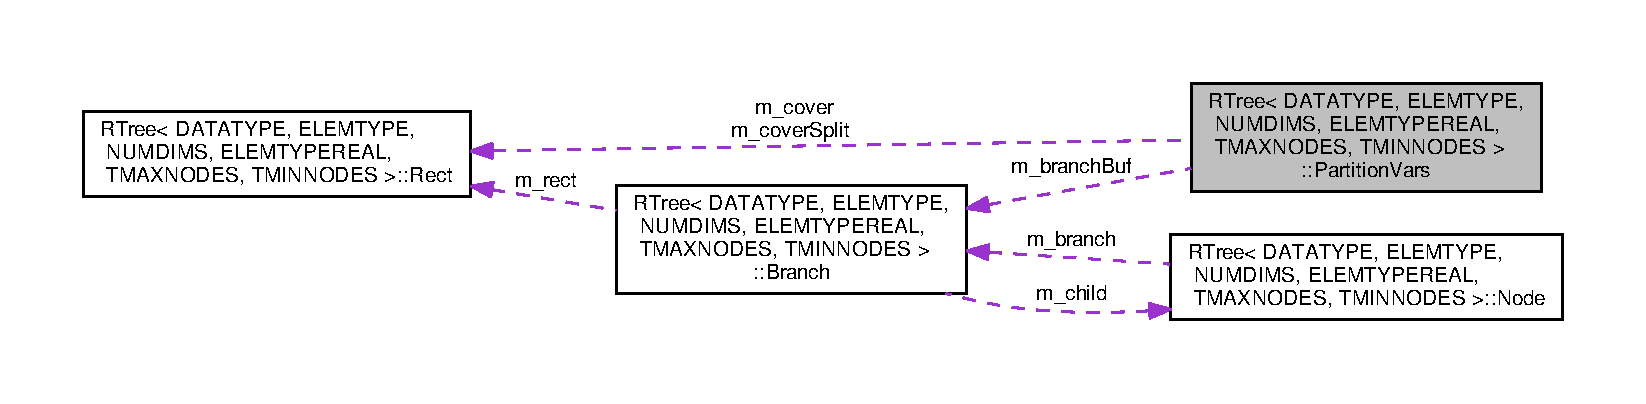
\includegraphics[width=350pt]{structRTree_1_1PartitionVars__coll__graph}
\end{center}
\end{figure}
\subsection*{Public Types}
\begin{DoxyCompactItemize}
\item 
enum \{ \hyperlink{structRTree_1_1PartitionVars_aa4395bc76d345f0a081c164bf68d4744acff1a730449e4b3de500024b4b6b6175}{N\-O\-T\-\_\-\-T\-A\-K\-E\-N} = -\/1
 \}
\end{DoxyCompactItemize}
\subsection*{Data Fields}
\begin{DoxyCompactItemize}
\item 
int \hyperlink{structRTree_1_1PartitionVars_a15b570f93f49884ccd637731d033da51}{m\-\_\-partition} \mbox{[}\hyperlink{classRTree_afaccb2e611f17ff46b623771ad7043d7ac05afe446df73fa67991e5199453a37f}{M\-A\-X\-N\-O\-D\-E\-S}+1\mbox{]}
\item 
int \hyperlink{structRTree_1_1PartitionVars_a145b95cd4210c8e2dbb2015d379906e4}{m\-\_\-total}
\item 
int \hyperlink{structRTree_1_1PartitionVars_a150d1fb0e446df4172c68eafbd0fc00d}{m\-\_\-min\-Fill}
\item 
int \hyperlink{structRTree_1_1PartitionVars_acbf70d46606cebe104471635d1c06c56}{m\-\_\-count} \mbox{[}2\mbox{]}
\item 
\hyperlink{structRTree_1_1Rect}{Rect} \hyperlink{structRTree_1_1PartitionVars_ab59894eefb7f3f6cc7254bbc90cd2570}{m\-\_\-cover} \mbox{[}2\mbox{]}
\item 
E\-L\-E\-M\-T\-Y\-P\-E\-R\-E\-A\-L \hyperlink{structRTree_1_1PartitionVars_aadf67cd0f0c071993f47b77b1e7a3b78}{m\-\_\-area} \mbox{[}2\mbox{]}
\item 
\hyperlink{structRTree_1_1Branch}{Branch} \hyperlink{structRTree_1_1PartitionVars_a73b5e398b4073ff923afaa765367958b}{m\-\_\-branch\-Buf} \mbox{[}\hyperlink{classRTree_afaccb2e611f17ff46b623771ad7043d7ac05afe446df73fa67991e5199453a37f}{M\-A\-X\-N\-O\-D\-E\-S}+1\mbox{]}
\item 
int \hyperlink{structRTree_1_1PartitionVars_abaaed8bac2d71bc6debadc5136078a0b}{m\-\_\-branch\-Count}
\item 
\hyperlink{structRTree_1_1Rect}{Rect} \hyperlink{structRTree_1_1PartitionVars_a61d9eaaae4128365146d923123f4b8d1}{m\-\_\-cover\-Split}
\item 
E\-L\-E\-M\-T\-Y\-P\-E\-R\-E\-A\-L \hyperlink{structRTree_1_1PartitionVars_ada65c4c4ae559f43f3b632bda1b7b7f2}{m\-\_\-cover\-Split\-Area}
\end{DoxyCompactItemize}


\subsection{Detailed Description}
\subsubsection*{template$<$class D\-A\-T\-A\-T\-Y\-P\-E, class E\-L\-E\-M\-T\-Y\-P\-E, int N\-U\-M\-D\-I\-M\-S, class E\-L\-E\-M\-T\-Y\-P\-E\-R\-E\-A\-L = E\-L\-E\-M\-T\-Y\-P\-E, int T\-M\-A\-X\-N\-O\-D\-E\-S = 8, int T\-M\-I\-N\-N\-O\-D\-E\-S = T\-M\-A\-X\-N\-O\-D\-E\-S / 2$>$struct R\-Tree$<$ D\-A\-T\-A\-T\-Y\-P\-E, E\-L\-E\-M\-T\-Y\-P\-E, N\-U\-M\-D\-I\-M\-S, E\-L\-E\-M\-T\-Y\-P\-E\-R\-E\-A\-L, T\-M\-A\-X\-N\-O\-D\-E\-S, T\-M\-I\-N\-N\-O\-D\-E\-S $>$\-::\-Partition\-Vars}

Variables for finding a split partition. 

\subsection{Member Enumeration Documentation}
\hypertarget{structRTree_1_1PartitionVars_aa4395bc76d345f0a081c164bf68d4744}{\subsubsection[{anonymous enum}]{\setlength{\rightskip}{0pt plus 5cm}template$<$class D\-A\-T\-A\-T\-Y\-P\-E, class E\-L\-E\-M\-T\-Y\-P\-E, int N\-U\-M\-D\-I\-M\-S, class E\-L\-E\-M\-T\-Y\-P\-E\-R\-E\-A\-L = E\-L\-E\-M\-T\-Y\-P\-E, int T\-M\-A\-X\-N\-O\-D\-E\-S = 8, int T\-M\-I\-N\-N\-O\-D\-E\-S = T\-M\-A\-X\-N\-O\-D\-E\-S / 2$>$ anonymous enum}}\label{structRTree_1_1PartitionVars_aa4395bc76d345f0a081c164bf68d4744}
\begin{Desc}
\item[Enumerator]\par
\begin{description}
\index{N\-O\-T\-\_\-\-T\-A\-K\-E\-N@{N\-O\-T\-\_\-\-T\-A\-K\-E\-N}!R\-Tree\-::\-Partition\-Vars@{R\-Tree\-::\-Partition\-Vars}}\index{R\-Tree\-::\-Partition\-Vars@{R\-Tree\-::\-Partition\-Vars}!N\-O\-T\-\_\-\-T\-A\-K\-E\-N@{N\-O\-T\-\_\-\-T\-A\-K\-E\-N}}\item[{\em 
\hypertarget{structRTree_1_1PartitionVars_aa4395bc76d345f0a081c164bf68d4744acff1a730449e4b3de500024b4b6b6175}{N\-O\-T\-\_\-\-T\-A\-K\-E\-N}\label{structRTree_1_1PartitionVars_aa4395bc76d345f0a081c164bf68d4744acff1a730449e4b3de500024b4b6b6175}
}]\end{description}
\end{Desc}


\subsection{Field Documentation}
\hypertarget{structRTree_1_1PartitionVars_aadf67cd0f0c071993f47b77b1e7a3b78}{\index{R\-Tree\-::\-Partition\-Vars@{R\-Tree\-::\-Partition\-Vars}!m\-\_\-area@{m\-\_\-area}}
\index{m\-\_\-area@{m\-\_\-area}!RTree::PartitionVars@{R\-Tree\-::\-Partition\-Vars}}
\subsubsection[{m\-\_\-area}]{\setlength{\rightskip}{0pt plus 5cm}template$<$class D\-A\-T\-A\-T\-Y\-P\-E, class E\-L\-E\-M\-T\-Y\-P\-E, int N\-U\-M\-D\-I\-M\-S, class E\-L\-E\-M\-T\-Y\-P\-E\-R\-E\-A\-L = E\-L\-E\-M\-T\-Y\-P\-E, int T\-M\-A\-X\-N\-O\-D\-E\-S = 8, int T\-M\-I\-N\-N\-O\-D\-E\-S = T\-M\-A\-X\-N\-O\-D\-E\-S / 2$>$ E\-L\-E\-M\-T\-Y\-P\-E\-R\-E\-A\-L {\bf R\-Tree}$<$ D\-A\-T\-A\-T\-Y\-P\-E, E\-L\-E\-M\-T\-Y\-P\-E, N\-U\-M\-D\-I\-M\-S, E\-L\-E\-M\-T\-Y\-P\-E\-R\-E\-A\-L, T\-M\-A\-X\-N\-O\-D\-E\-S, T\-M\-I\-N\-N\-O\-D\-E\-S $>$\-::Partition\-Vars\-::m\-\_\-area\mbox{[}2\mbox{]}}}\label{structRTree_1_1PartitionVars_aadf67cd0f0c071993f47b77b1e7a3b78}
\hypertarget{structRTree_1_1PartitionVars_a73b5e398b4073ff923afaa765367958b}{\index{R\-Tree\-::\-Partition\-Vars@{R\-Tree\-::\-Partition\-Vars}!m\-\_\-branch\-Buf@{m\-\_\-branch\-Buf}}
\index{m\-\_\-branch\-Buf@{m\-\_\-branch\-Buf}!RTree::PartitionVars@{R\-Tree\-::\-Partition\-Vars}}
\subsubsection[{m\-\_\-branch\-Buf}]{\setlength{\rightskip}{0pt plus 5cm}template$<$class D\-A\-T\-A\-T\-Y\-P\-E, class E\-L\-E\-M\-T\-Y\-P\-E, int N\-U\-M\-D\-I\-M\-S, class E\-L\-E\-M\-T\-Y\-P\-E\-R\-E\-A\-L = E\-L\-E\-M\-T\-Y\-P\-E, int T\-M\-A\-X\-N\-O\-D\-E\-S = 8, int T\-M\-I\-N\-N\-O\-D\-E\-S = T\-M\-A\-X\-N\-O\-D\-E\-S / 2$>$ {\bf Branch} {\bf R\-Tree}$<$ D\-A\-T\-A\-T\-Y\-P\-E, E\-L\-E\-M\-T\-Y\-P\-E, N\-U\-M\-D\-I\-M\-S, E\-L\-E\-M\-T\-Y\-P\-E\-R\-E\-A\-L, T\-M\-A\-X\-N\-O\-D\-E\-S, T\-M\-I\-N\-N\-O\-D\-E\-S $>$\-::Partition\-Vars\-::m\-\_\-branch\-Buf\mbox{[}{\bf M\-A\-X\-N\-O\-D\-E\-S}+1\mbox{]}}}\label{structRTree_1_1PartitionVars_a73b5e398b4073ff923afaa765367958b}
\hypertarget{structRTree_1_1PartitionVars_abaaed8bac2d71bc6debadc5136078a0b}{\index{R\-Tree\-::\-Partition\-Vars@{R\-Tree\-::\-Partition\-Vars}!m\-\_\-branch\-Count@{m\-\_\-branch\-Count}}
\index{m\-\_\-branch\-Count@{m\-\_\-branch\-Count}!RTree::PartitionVars@{R\-Tree\-::\-Partition\-Vars}}
\subsubsection[{m\-\_\-branch\-Count}]{\setlength{\rightskip}{0pt plus 5cm}template$<$class D\-A\-T\-A\-T\-Y\-P\-E, class E\-L\-E\-M\-T\-Y\-P\-E, int N\-U\-M\-D\-I\-M\-S, class E\-L\-E\-M\-T\-Y\-P\-E\-R\-E\-A\-L = E\-L\-E\-M\-T\-Y\-P\-E, int T\-M\-A\-X\-N\-O\-D\-E\-S = 8, int T\-M\-I\-N\-N\-O\-D\-E\-S = T\-M\-A\-X\-N\-O\-D\-E\-S / 2$>$ int {\bf R\-Tree}$<$ D\-A\-T\-A\-T\-Y\-P\-E, E\-L\-E\-M\-T\-Y\-P\-E, N\-U\-M\-D\-I\-M\-S, E\-L\-E\-M\-T\-Y\-P\-E\-R\-E\-A\-L, T\-M\-A\-X\-N\-O\-D\-E\-S, T\-M\-I\-N\-N\-O\-D\-E\-S $>$\-::Partition\-Vars\-::m\-\_\-branch\-Count}}\label{structRTree_1_1PartitionVars_abaaed8bac2d71bc6debadc5136078a0b}
\hypertarget{structRTree_1_1PartitionVars_acbf70d46606cebe104471635d1c06c56}{\index{R\-Tree\-::\-Partition\-Vars@{R\-Tree\-::\-Partition\-Vars}!m\-\_\-count@{m\-\_\-count}}
\index{m\-\_\-count@{m\-\_\-count}!RTree::PartitionVars@{R\-Tree\-::\-Partition\-Vars}}
\subsubsection[{m\-\_\-count}]{\setlength{\rightskip}{0pt plus 5cm}template$<$class D\-A\-T\-A\-T\-Y\-P\-E, class E\-L\-E\-M\-T\-Y\-P\-E, int N\-U\-M\-D\-I\-M\-S, class E\-L\-E\-M\-T\-Y\-P\-E\-R\-E\-A\-L = E\-L\-E\-M\-T\-Y\-P\-E, int T\-M\-A\-X\-N\-O\-D\-E\-S = 8, int T\-M\-I\-N\-N\-O\-D\-E\-S = T\-M\-A\-X\-N\-O\-D\-E\-S / 2$>$ int {\bf R\-Tree}$<$ D\-A\-T\-A\-T\-Y\-P\-E, E\-L\-E\-M\-T\-Y\-P\-E, N\-U\-M\-D\-I\-M\-S, E\-L\-E\-M\-T\-Y\-P\-E\-R\-E\-A\-L, T\-M\-A\-X\-N\-O\-D\-E\-S, T\-M\-I\-N\-N\-O\-D\-E\-S $>$\-::Partition\-Vars\-::m\-\_\-count\mbox{[}2\mbox{]}}}\label{structRTree_1_1PartitionVars_acbf70d46606cebe104471635d1c06c56}
\hypertarget{structRTree_1_1PartitionVars_ab59894eefb7f3f6cc7254bbc90cd2570}{\index{R\-Tree\-::\-Partition\-Vars@{R\-Tree\-::\-Partition\-Vars}!m\-\_\-cover@{m\-\_\-cover}}
\index{m\-\_\-cover@{m\-\_\-cover}!RTree::PartitionVars@{R\-Tree\-::\-Partition\-Vars}}
\subsubsection[{m\-\_\-cover}]{\setlength{\rightskip}{0pt plus 5cm}template$<$class D\-A\-T\-A\-T\-Y\-P\-E, class E\-L\-E\-M\-T\-Y\-P\-E, int N\-U\-M\-D\-I\-M\-S, class E\-L\-E\-M\-T\-Y\-P\-E\-R\-E\-A\-L = E\-L\-E\-M\-T\-Y\-P\-E, int T\-M\-A\-X\-N\-O\-D\-E\-S = 8, int T\-M\-I\-N\-N\-O\-D\-E\-S = T\-M\-A\-X\-N\-O\-D\-E\-S / 2$>$ {\bf Rect} {\bf R\-Tree}$<$ D\-A\-T\-A\-T\-Y\-P\-E, E\-L\-E\-M\-T\-Y\-P\-E, N\-U\-M\-D\-I\-M\-S, E\-L\-E\-M\-T\-Y\-P\-E\-R\-E\-A\-L, T\-M\-A\-X\-N\-O\-D\-E\-S, T\-M\-I\-N\-N\-O\-D\-E\-S $>$\-::Partition\-Vars\-::m\-\_\-cover\mbox{[}2\mbox{]}}}\label{structRTree_1_1PartitionVars_ab59894eefb7f3f6cc7254bbc90cd2570}
\hypertarget{structRTree_1_1PartitionVars_a61d9eaaae4128365146d923123f4b8d1}{\index{R\-Tree\-::\-Partition\-Vars@{R\-Tree\-::\-Partition\-Vars}!m\-\_\-cover\-Split@{m\-\_\-cover\-Split}}
\index{m\-\_\-cover\-Split@{m\-\_\-cover\-Split}!RTree::PartitionVars@{R\-Tree\-::\-Partition\-Vars}}
\subsubsection[{m\-\_\-cover\-Split}]{\setlength{\rightskip}{0pt plus 5cm}template$<$class D\-A\-T\-A\-T\-Y\-P\-E, class E\-L\-E\-M\-T\-Y\-P\-E, int N\-U\-M\-D\-I\-M\-S, class E\-L\-E\-M\-T\-Y\-P\-E\-R\-E\-A\-L = E\-L\-E\-M\-T\-Y\-P\-E, int T\-M\-A\-X\-N\-O\-D\-E\-S = 8, int T\-M\-I\-N\-N\-O\-D\-E\-S = T\-M\-A\-X\-N\-O\-D\-E\-S / 2$>$ {\bf Rect} {\bf R\-Tree}$<$ D\-A\-T\-A\-T\-Y\-P\-E, E\-L\-E\-M\-T\-Y\-P\-E, N\-U\-M\-D\-I\-M\-S, E\-L\-E\-M\-T\-Y\-P\-E\-R\-E\-A\-L, T\-M\-A\-X\-N\-O\-D\-E\-S, T\-M\-I\-N\-N\-O\-D\-E\-S $>$\-::Partition\-Vars\-::m\-\_\-cover\-Split}}\label{structRTree_1_1PartitionVars_a61d9eaaae4128365146d923123f4b8d1}
\hypertarget{structRTree_1_1PartitionVars_ada65c4c4ae559f43f3b632bda1b7b7f2}{\index{R\-Tree\-::\-Partition\-Vars@{R\-Tree\-::\-Partition\-Vars}!m\-\_\-cover\-Split\-Area@{m\-\_\-cover\-Split\-Area}}
\index{m\-\_\-cover\-Split\-Area@{m\-\_\-cover\-Split\-Area}!RTree::PartitionVars@{R\-Tree\-::\-Partition\-Vars}}
\subsubsection[{m\-\_\-cover\-Split\-Area}]{\setlength{\rightskip}{0pt plus 5cm}template$<$class D\-A\-T\-A\-T\-Y\-P\-E, class E\-L\-E\-M\-T\-Y\-P\-E, int N\-U\-M\-D\-I\-M\-S, class E\-L\-E\-M\-T\-Y\-P\-E\-R\-E\-A\-L = E\-L\-E\-M\-T\-Y\-P\-E, int T\-M\-A\-X\-N\-O\-D\-E\-S = 8, int T\-M\-I\-N\-N\-O\-D\-E\-S = T\-M\-A\-X\-N\-O\-D\-E\-S / 2$>$ E\-L\-E\-M\-T\-Y\-P\-E\-R\-E\-A\-L {\bf R\-Tree}$<$ D\-A\-T\-A\-T\-Y\-P\-E, E\-L\-E\-M\-T\-Y\-P\-E, N\-U\-M\-D\-I\-M\-S, E\-L\-E\-M\-T\-Y\-P\-E\-R\-E\-A\-L, T\-M\-A\-X\-N\-O\-D\-E\-S, T\-M\-I\-N\-N\-O\-D\-E\-S $>$\-::Partition\-Vars\-::m\-\_\-cover\-Split\-Area}}\label{structRTree_1_1PartitionVars_ada65c4c4ae559f43f3b632bda1b7b7f2}
\hypertarget{structRTree_1_1PartitionVars_a150d1fb0e446df4172c68eafbd0fc00d}{\index{R\-Tree\-::\-Partition\-Vars@{R\-Tree\-::\-Partition\-Vars}!m\-\_\-min\-Fill@{m\-\_\-min\-Fill}}
\index{m\-\_\-min\-Fill@{m\-\_\-min\-Fill}!RTree::PartitionVars@{R\-Tree\-::\-Partition\-Vars}}
\subsubsection[{m\-\_\-min\-Fill}]{\setlength{\rightskip}{0pt plus 5cm}template$<$class D\-A\-T\-A\-T\-Y\-P\-E, class E\-L\-E\-M\-T\-Y\-P\-E, int N\-U\-M\-D\-I\-M\-S, class E\-L\-E\-M\-T\-Y\-P\-E\-R\-E\-A\-L = E\-L\-E\-M\-T\-Y\-P\-E, int T\-M\-A\-X\-N\-O\-D\-E\-S = 8, int T\-M\-I\-N\-N\-O\-D\-E\-S = T\-M\-A\-X\-N\-O\-D\-E\-S / 2$>$ int {\bf R\-Tree}$<$ D\-A\-T\-A\-T\-Y\-P\-E, E\-L\-E\-M\-T\-Y\-P\-E, N\-U\-M\-D\-I\-M\-S, E\-L\-E\-M\-T\-Y\-P\-E\-R\-E\-A\-L, T\-M\-A\-X\-N\-O\-D\-E\-S, T\-M\-I\-N\-N\-O\-D\-E\-S $>$\-::Partition\-Vars\-::m\-\_\-min\-Fill}}\label{structRTree_1_1PartitionVars_a150d1fb0e446df4172c68eafbd0fc00d}
\hypertarget{structRTree_1_1PartitionVars_a15b570f93f49884ccd637731d033da51}{\index{R\-Tree\-::\-Partition\-Vars@{R\-Tree\-::\-Partition\-Vars}!m\-\_\-partition@{m\-\_\-partition}}
\index{m\-\_\-partition@{m\-\_\-partition}!RTree::PartitionVars@{R\-Tree\-::\-Partition\-Vars}}
\subsubsection[{m\-\_\-partition}]{\setlength{\rightskip}{0pt plus 5cm}template$<$class D\-A\-T\-A\-T\-Y\-P\-E, class E\-L\-E\-M\-T\-Y\-P\-E, int N\-U\-M\-D\-I\-M\-S, class E\-L\-E\-M\-T\-Y\-P\-E\-R\-E\-A\-L = E\-L\-E\-M\-T\-Y\-P\-E, int T\-M\-A\-X\-N\-O\-D\-E\-S = 8, int T\-M\-I\-N\-N\-O\-D\-E\-S = T\-M\-A\-X\-N\-O\-D\-E\-S / 2$>$ int {\bf R\-Tree}$<$ D\-A\-T\-A\-T\-Y\-P\-E, E\-L\-E\-M\-T\-Y\-P\-E, N\-U\-M\-D\-I\-M\-S, E\-L\-E\-M\-T\-Y\-P\-E\-R\-E\-A\-L, T\-M\-A\-X\-N\-O\-D\-E\-S, T\-M\-I\-N\-N\-O\-D\-E\-S $>$\-::Partition\-Vars\-::m\-\_\-partition\mbox{[}{\bf M\-A\-X\-N\-O\-D\-E\-S}+1\mbox{]}}}\label{structRTree_1_1PartitionVars_a15b570f93f49884ccd637731d033da51}
\hypertarget{structRTree_1_1PartitionVars_a145b95cd4210c8e2dbb2015d379906e4}{\index{R\-Tree\-::\-Partition\-Vars@{R\-Tree\-::\-Partition\-Vars}!m\-\_\-total@{m\-\_\-total}}
\index{m\-\_\-total@{m\-\_\-total}!RTree::PartitionVars@{R\-Tree\-::\-Partition\-Vars}}
\subsubsection[{m\-\_\-total}]{\setlength{\rightskip}{0pt plus 5cm}template$<$class D\-A\-T\-A\-T\-Y\-P\-E, class E\-L\-E\-M\-T\-Y\-P\-E, int N\-U\-M\-D\-I\-M\-S, class E\-L\-E\-M\-T\-Y\-P\-E\-R\-E\-A\-L = E\-L\-E\-M\-T\-Y\-P\-E, int T\-M\-A\-X\-N\-O\-D\-E\-S = 8, int T\-M\-I\-N\-N\-O\-D\-E\-S = T\-M\-A\-X\-N\-O\-D\-E\-S / 2$>$ int {\bf R\-Tree}$<$ D\-A\-T\-A\-T\-Y\-P\-E, E\-L\-E\-M\-T\-Y\-P\-E, N\-U\-M\-D\-I\-M\-S, E\-L\-E\-M\-T\-Y\-P\-E\-R\-E\-A\-L, T\-M\-A\-X\-N\-O\-D\-E\-S, T\-M\-I\-N\-N\-O\-D\-E\-S $>$\-::Partition\-Vars\-::m\-\_\-total}}\label{structRTree_1_1PartitionVars_a145b95cd4210c8e2dbb2015d379906e4}


The documentation for this struct was generated from the following file\-:\begin{DoxyCompactItemize}
\item 
\hyperlink{RTree_8h}{R\-Tree.\-h}\end{DoxyCompactItemize}

\hypertarget{structQueryRect}{\section{Query\-Rect Struct Reference}
\label{structQueryRect}\index{Query\-Rect@{Query\-Rect}}
}


{\ttfamily \#include \char`\"{}structs.\-h\char`\"{}}

\subsection*{Public Member Functions}
\begin{DoxyCompactItemize}
\item 
\hyperlink{structQueryRect_a747941fb202e6b876ed797f5399a4cd1}{Query\-Rect} ()
\item 
void \hyperlink{structQueryRect_aee38688f3849a165117c169b6e326fc9}{Create\-M\-B\-B} ()
\end{DoxyCompactItemize}
\subsection*{Data Fields}
\begin{DoxyCompactItemize}
\item 
double \hyperlink{structQueryRect_af589b8614fd373e1777e51f19fbb2f50}{P1} \mbox{[}2\mbox{]}
\item 
double \hyperlink{structQueryRect_aa0f3a5df0448d5632db92c91a5a00e37}{P2} \mbox{[}2\mbox{]}
\item 
double \hyperlink{structQueryRect_af2cf3779c1154df6ac056c08a440f1a9}{M\-B\-B\-\_\-min} \mbox{[}2\mbox{]}
\item 
double \hyperlink{structQueryRect_a79ee9ad46493db3f4508b6bdbd7fbaad}{M\-B\-B\-\_\-max} \mbox{[}2\mbox{]}
\end{DoxyCompactItemize}


\subsection{Detailed Description}
M\-B\-B for querying the R-\/tree 

\subsection{Constructor \& Destructor Documentation}
\hypertarget{structQueryRect_a747941fb202e6b876ed797f5399a4cd1}{\index{Query\-Rect@{Query\-Rect}!Query\-Rect@{Query\-Rect}}
\index{Query\-Rect@{Query\-Rect}!QueryRect@{Query\-Rect}}
\subsubsection[{Query\-Rect}]{\setlength{\rightskip}{0pt plus 5cm}Query\-Rect\-::\-Query\-Rect (
\begin{DoxyParamCaption}
{}
\end{DoxyParamCaption}
)\hspace{0.3cm}{\ttfamily [inline]}}}\label{structQueryRect_a747941fb202e6b876ed797f5399a4cd1}


\subsection{Member Function Documentation}
\hypertarget{structQueryRect_aee38688f3849a165117c169b6e326fc9}{\index{Query\-Rect@{Query\-Rect}!Create\-M\-B\-B@{Create\-M\-B\-B}}
\index{Create\-M\-B\-B@{Create\-M\-B\-B}!QueryRect@{Query\-Rect}}
\subsubsection[{Create\-M\-B\-B}]{\setlength{\rightskip}{0pt plus 5cm}void Query\-Rect\-::\-Create\-M\-B\-B (
\begin{DoxyParamCaption}
{}
\end{DoxyParamCaption}
)\hspace{0.3cm}{\ttfamily [inline]}}}\label{structQueryRect_aee38688f3849a165117c169b6e326fc9}


\subsection{Field Documentation}
\hypertarget{structQueryRect_a79ee9ad46493db3f4508b6bdbd7fbaad}{\index{Query\-Rect@{Query\-Rect}!M\-B\-B\-\_\-max@{M\-B\-B\-\_\-max}}
\index{M\-B\-B\-\_\-max@{M\-B\-B\-\_\-max}!QueryRect@{Query\-Rect}}
\subsubsection[{M\-B\-B\-\_\-max}]{\setlength{\rightskip}{0pt plus 5cm}double Query\-Rect\-::\-M\-B\-B\-\_\-max\mbox{[}2\mbox{]}}}\label{structQueryRect_a79ee9ad46493db3f4508b6bdbd7fbaad}
\hypertarget{structQueryRect_af2cf3779c1154df6ac056c08a440f1a9}{\index{Query\-Rect@{Query\-Rect}!M\-B\-B\-\_\-min@{M\-B\-B\-\_\-min}}
\index{M\-B\-B\-\_\-min@{M\-B\-B\-\_\-min}!QueryRect@{Query\-Rect}}
\subsubsection[{M\-B\-B\-\_\-min}]{\setlength{\rightskip}{0pt plus 5cm}double Query\-Rect\-::\-M\-B\-B\-\_\-min\mbox{[}2\mbox{]}}}\label{structQueryRect_af2cf3779c1154df6ac056c08a440f1a9}
\hypertarget{structQueryRect_af589b8614fd373e1777e51f19fbb2f50}{\index{Query\-Rect@{Query\-Rect}!P1@{P1}}
\index{P1@{P1}!QueryRect@{Query\-Rect}}
\subsubsection[{P1}]{\setlength{\rightskip}{0pt plus 5cm}double Query\-Rect\-::\-P1\mbox{[}2\mbox{]}}}\label{structQueryRect_af589b8614fd373e1777e51f19fbb2f50}
\hypertarget{structQueryRect_aa0f3a5df0448d5632db92c91a5a00e37}{\index{Query\-Rect@{Query\-Rect}!P2@{P2}}
\index{P2@{P2}!QueryRect@{Query\-Rect}}
\subsubsection[{P2}]{\setlength{\rightskip}{0pt plus 5cm}double Query\-Rect\-::\-P2\mbox{[}2\mbox{]}}}\label{structQueryRect_aa0f3a5df0448d5632db92c91a5a00e37}


The documentation for this struct was generated from the following file\-:\begin{DoxyCompactItemize}
\item 
\hyperlink{structs_8h}{structs.\-h}\end{DoxyCompactItemize}

\hypertarget{structRTree_1_1Rect}{\section{R\-Tree$<$ D\-A\-T\-A\-T\-Y\-P\-E, E\-L\-E\-M\-T\-Y\-P\-E, N\-U\-M\-D\-I\-M\-S, E\-L\-E\-M\-T\-Y\-P\-E\-R\-E\-A\-L, T\-M\-A\-X\-N\-O\-D\-E\-S, T\-M\-I\-N\-N\-O\-D\-E\-S $>$\-:\-:Rect Struct Reference}
\label{structRTree_1_1Rect}\index{R\-Tree$<$ D\-A\-T\-A\-T\-Y\-P\-E, E\-L\-E\-M\-T\-Y\-P\-E, N\-U\-M\-D\-I\-M\-S, E\-L\-E\-M\-T\-Y\-P\-E\-R\-E\-A\-L, T\-M\-A\-X\-N\-O\-D\-E\-S, T\-M\-I\-N\-N\-O\-D\-E\-S $>$\-::\-Rect@{R\-Tree$<$ D\-A\-T\-A\-T\-Y\-P\-E, E\-L\-E\-M\-T\-Y\-P\-E, N\-U\-M\-D\-I\-M\-S, E\-L\-E\-M\-T\-Y\-P\-E\-R\-E\-A\-L, T\-M\-A\-X\-N\-O\-D\-E\-S, T\-M\-I\-N\-N\-O\-D\-E\-S $>$\-::\-Rect}}
}


Minimal bounding rectangle (n-\/dimensional)  




{\ttfamily \#include \char`\"{}R\-Tree.\-h\char`\"{}}

\subsection*{Data Fields}
\begin{DoxyCompactItemize}
\item 
E\-L\-E\-M\-T\-Y\-P\-E \hyperlink{structRTree_1_1Rect_a2b5b254493aba27b30fe6fc8df151ed5}{m\-\_\-min} \mbox{[}N\-U\-M\-D\-I\-M\-S\mbox{]}
\begin{DoxyCompactList}\small\item\em Min dimensions of bounding box. \end{DoxyCompactList}\item 
E\-L\-E\-M\-T\-Y\-P\-E \hyperlink{structRTree_1_1Rect_a6570c2a5a16b19b0d08cd1eaa224961b}{m\-\_\-max} \mbox{[}N\-U\-M\-D\-I\-M\-S\mbox{]}
\begin{DoxyCompactList}\small\item\em Max dimensions of bounding box. \end{DoxyCompactList}\item 
D\-A\-T\-A\-T\-Y\-P\-E \hyperlink{structRTree_1_1Rect_ae30aa6041e1f115d9f779cc6f127f6f4}{m\-\_\-traj\-\_\-id}
\item 
D\-A\-T\-A\-T\-Y\-P\-E \hyperlink{structRTree_1_1Rect_a36196729bcd01906974001af26423cb7}{m\-\_\-segment\-\_\-id}
\begin{DoxyCompactList}\small\item\em mine\-: F\-O\-R T\-R\-A\-J\-E\-C\-T\-O\-R\-Y I\-D \end{DoxyCompactList}\end{DoxyCompactItemize}


\subsection{Detailed Description}
\subsubsection*{template$<$class D\-A\-T\-A\-T\-Y\-P\-E, class E\-L\-E\-M\-T\-Y\-P\-E, int N\-U\-M\-D\-I\-M\-S, class E\-L\-E\-M\-T\-Y\-P\-E\-R\-E\-A\-L = E\-L\-E\-M\-T\-Y\-P\-E, int T\-M\-A\-X\-N\-O\-D\-E\-S = 8, int T\-M\-I\-N\-N\-O\-D\-E\-S = T\-M\-A\-X\-N\-O\-D\-E\-S / 2$>$struct R\-Tree$<$ D\-A\-T\-A\-T\-Y\-P\-E, E\-L\-E\-M\-T\-Y\-P\-E, N\-U\-M\-D\-I\-M\-S, E\-L\-E\-M\-T\-Y\-P\-E\-R\-E\-A\-L, T\-M\-A\-X\-N\-O\-D\-E\-S, T\-M\-I\-N\-N\-O\-D\-E\-S $>$\-::\-Rect}

Minimal bounding rectangle (n-\/dimensional) 

\subsection{Field Documentation}
\hypertarget{structRTree_1_1Rect_a6570c2a5a16b19b0d08cd1eaa224961b}{\index{R\-Tree\-::\-Rect@{R\-Tree\-::\-Rect}!m\-\_\-max@{m\-\_\-max}}
\index{m\-\_\-max@{m\-\_\-max}!RTree::Rect@{R\-Tree\-::\-Rect}}
\subsubsection[{m\-\_\-max}]{\setlength{\rightskip}{0pt plus 5cm}template$<$class D\-A\-T\-A\-T\-Y\-P\-E, class E\-L\-E\-M\-T\-Y\-P\-E, int N\-U\-M\-D\-I\-M\-S, class E\-L\-E\-M\-T\-Y\-P\-E\-R\-E\-A\-L = E\-L\-E\-M\-T\-Y\-P\-E, int T\-M\-A\-X\-N\-O\-D\-E\-S = 8, int T\-M\-I\-N\-N\-O\-D\-E\-S = T\-M\-A\-X\-N\-O\-D\-E\-S / 2$>$ E\-L\-E\-M\-T\-Y\-P\-E {\bf R\-Tree}$<$ D\-A\-T\-A\-T\-Y\-P\-E, E\-L\-E\-M\-T\-Y\-P\-E, N\-U\-M\-D\-I\-M\-S, E\-L\-E\-M\-T\-Y\-P\-E\-R\-E\-A\-L, T\-M\-A\-X\-N\-O\-D\-E\-S, T\-M\-I\-N\-N\-O\-D\-E\-S $>$\-::Rect\-::m\-\_\-max\mbox{[}N\-U\-M\-D\-I\-M\-S\mbox{]}}}\label{structRTree_1_1Rect_a6570c2a5a16b19b0d08cd1eaa224961b}


Max dimensions of bounding box. 

\hypertarget{structRTree_1_1Rect_a2b5b254493aba27b30fe6fc8df151ed5}{\index{R\-Tree\-::\-Rect@{R\-Tree\-::\-Rect}!m\-\_\-min@{m\-\_\-min}}
\index{m\-\_\-min@{m\-\_\-min}!RTree::Rect@{R\-Tree\-::\-Rect}}
\subsubsection[{m\-\_\-min}]{\setlength{\rightskip}{0pt plus 5cm}template$<$class D\-A\-T\-A\-T\-Y\-P\-E, class E\-L\-E\-M\-T\-Y\-P\-E, int N\-U\-M\-D\-I\-M\-S, class E\-L\-E\-M\-T\-Y\-P\-E\-R\-E\-A\-L = E\-L\-E\-M\-T\-Y\-P\-E, int T\-M\-A\-X\-N\-O\-D\-E\-S = 8, int T\-M\-I\-N\-N\-O\-D\-E\-S = T\-M\-A\-X\-N\-O\-D\-E\-S / 2$>$ E\-L\-E\-M\-T\-Y\-P\-E {\bf R\-Tree}$<$ D\-A\-T\-A\-T\-Y\-P\-E, E\-L\-E\-M\-T\-Y\-P\-E, N\-U\-M\-D\-I\-M\-S, E\-L\-E\-M\-T\-Y\-P\-E\-R\-E\-A\-L, T\-M\-A\-X\-N\-O\-D\-E\-S, T\-M\-I\-N\-N\-O\-D\-E\-S $>$\-::Rect\-::m\-\_\-min\mbox{[}N\-U\-M\-D\-I\-M\-S\mbox{]}}}\label{structRTree_1_1Rect_a2b5b254493aba27b30fe6fc8df151ed5}


Min dimensions of bounding box. 

\hypertarget{structRTree_1_1Rect_a36196729bcd01906974001af26423cb7}{\index{R\-Tree\-::\-Rect@{R\-Tree\-::\-Rect}!m\-\_\-segment\-\_\-id@{m\-\_\-segment\-\_\-id}}
\index{m\-\_\-segment\-\_\-id@{m\-\_\-segment\-\_\-id}!RTree::Rect@{R\-Tree\-::\-Rect}}
\subsubsection[{m\-\_\-segment\-\_\-id}]{\setlength{\rightskip}{0pt plus 5cm}template$<$class D\-A\-T\-A\-T\-Y\-P\-E, class E\-L\-E\-M\-T\-Y\-P\-E, int N\-U\-M\-D\-I\-M\-S, class E\-L\-E\-M\-T\-Y\-P\-E\-R\-E\-A\-L = E\-L\-E\-M\-T\-Y\-P\-E, int T\-M\-A\-X\-N\-O\-D\-E\-S = 8, int T\-M\-I\-N\-N\-O\-D\-E\-S = T\-M\-A\-X\-N\-O\-D\-E\-S / 2$>$ D\-A\-T\-A\-T\-Y\-P\-E {\bf R\-Tree}$<$ D\-A\-T\-A\-T\-Y\-P\-E, E\-L\-E\-M\-T\-Y\-P\-E, N\-U\-M\-D\-I\-M\-S, E\-L\-E\-M\-T\-Y\-P\-E\-R\-E\-A\-L, T\-M\-A\-X\-N\-O\-D\-E\-S, T\-M\-I\-N\-N\-O\-D\-E\-S $>$\-::Rect\-::m\-\_\-segment\-\_\-id}}\label{structRTree_1_1Rect_a36196729bcd01906974001af26423cb7}


mine\-: F\-O\-R T\-R\-A\-J\-E\-C\-T\-O\-R\-Y I\-D 

\hypertarget{structRTree_1_1Rect_ae30aa6041e1f115d9f779cc6f127f6f4}{\index{R\-Tree\-::\-Rect@{R\-Tree\-::\-Rect}!m\-\_\-traj\-\_\-id@{m\-\_\-traj\-\_\-id}}
\index{m\-\_\-traj\-\_\-id@{m\-\_\-traj\-\_\-id}!RTree::Rect@{R\-Tree\-::\-Rect}}
\subsubsection[{m\-\_\-traj\-\_\-id}]{\setlength{\rightskip}{0pt plus 5cm}template$<$class D\-A\-T\-A\-T\-Y\-P\-E, class E\-L\-E\-M\-T\-Y\-P\-E, int N\-U\-M\-D\-I\-M\-S, class E\-L\-E\-M\-T\-Y\-P\-E\-R\-E\-A\-L = E\-L\-E\-M\-T\-Y\-P\-E, int T\-M\-A\-X\-N\-O\-D\-E\-S = 8, int T\-M\-I\-N\-N\-O\-D\-E\-S = T\-M\-A\-X\-N\-O\-D\-E\-S / 2$>$ D\-A\-T\-A\-T\-Y\-P\-E {\bf R\-Tree}$<$ D\-A\-T\-A\-T\-Y\-P\-E, E\-L\-E\-M\-T\-Y\-P\-E, N\-U\-M\-D\-I\-M\-S, E\-L\-E\-M\-T\-Y\-P\-E\-R\-E\-A\-L, T\-M\-A\-X\-N\-O\-D\-E\-S, T\-M\-I\-N\-N\-O\-D\-E\-S $>$\-::Rect\-::m\-\_\-traj\-\_\-id}}\label{structRTree_1_1Rect_ae30aa6041e1f115d9f779cc6f127f6f4}


The documentation for this struct was generated from the following file\-:\begin{DoxyCompactItemize}
\item 
\hyperlink{RTree_8h}{R\-Tree.\-h}\end{DoxyCompactItemize}

\hypertarget{structRect}{\section{Rect Struct Reference}
\label{structRect}\index{Rect@{Rect}}
}


{\ttfamily \#include \char`\"{}structs.\-h\char`\"{}}

\subsection*{Public Member Functions}
\begin{DoxyCompactItemize}
\item 
\hyperlink{structRect_a911e531b86de33734dd7de3456722115}{Rect} ()
\item 
void \hyperlink{structRect_ab9d4fbb9ca363982331de4e161c0a1b6}{Create\-M\-B\-B} ()
\end{DoxyCompactItemize}
\subsection*{Data Fields}
\begin{DoxyCompactItemize}
\item 
double \hyperlink{structRect_a9f7ff3649a3f3fb57e50216562cac766}{P1} \mbox{[}2\mbox{]}
\item 
double \hyperlink{structRect_a1c06137712547caecbc8610284935cfd}{M\-B\-B\-\_\-min} \mbox{[}2\mbox{]}
\item 
double \hyperlink{structRect_a1c17b7e7f839fa2da165b1d9b29e0513}{M\-B\-B\-\_\-max} \mbox{[}2\mbox{]}
\item 
int \hyperlink{structRect_ae80df46c77b1ce01bfff606424f07d20}{pid}
\end{DoxyCompactItemize}


\subsection{Detailed Description}
Used for the index of point objects. They make the M\-B\-Bs that are inserted into the tree (2-\/\-D M\-B\-Bs) 

\subsection{Constructor \& Destructor Documentation}
\hypertarget{structRect_a911e531b86de33734dd7de3456722115}{\index{Rect@{Rect}!Rect@{Rect}}
\index{Rect@{Rect}!Rect@{Rect}}
\subsubsection[{Rect}]{\setlength{\rightskip}{0pt plus 5cm}Rect\-::\-Rect (
\begin{DoxyParamCaption}
{}
\end{DoxyParamCaption}
)\hspace{0.3cm}{\ttfamily [inline]}}}\label{structRect_a911e531b86de33734dd7de3456722115}


\subsection{Member Function Documentation}
\hypertarget{structRect_ab9d4fbb9ca363982331de4e161c0a1b6}{\index{Rect@{Rect}!Create\-M\-B\-B@{Create\-M\-B\-B}}
\index{Create\-M\-B\-B@{Create\-M\-B\-B}!Rect@{Rect}}
\subsubsection[{Create\-M\-B\-B}]{\setlength{\rightskip}{0pt plus 5cm}void Rect\-::\-Create\-M\-B\-B (
\begin{DoxyParamCaption}
{}
\end{DoxyParamCaption}
)\hspace{0.3cm}{\ttfamily [inline]}}}\label{structRect_ab9d4fbb9ca363982331de4e161c0a1b6}


\subsection{Field Documentation}
\hypertarget{structRect_a1c17b7e7f839fa2da165b1d9b29e0513}{\index{Rect@{Rect}!M\-B\-B\-\_\-max@{M\-B\-B\-\_\-max}}
\index{M\-B\-B\-\_\-max@{M\-B\-B\-\_\-max}!Rect@{Rect}}
\subsubsection[{M\-B\-B\-\_\-max}]{\setlength{\rightskip}{0pt plus 5cm}double Rect\-::\-M\-B\-B\-\_\-max\mbox{[}2\mbox{]}}}\label{structRect_a1c17b7e7f839fa2da165b1d9b29e0513}
\hypertarget{structRect_a1c06137712547caecbc8610284935cfd}{\index{Rect@{Rect}!M\-B\-B\-\_\-min@{M\-B\-B\-\_\-min}}
\index{M\-B\-B\-\_\-min@{M\-B\-B\-\_\-min}!Rect@{Rect}}
\subsubsection[{M\-B\-B\-\_\-min}]{\setlength{\rightskip}{0pt plus 5cm}double Rect\-::\-M\-B\-B\-\_\-min\mbox{[}2\mbox{]}}}\label{structRect_a1c06137712547caecbc8610284935cfd}
\hypertarget{structRect_a9f7ff3649a3f3fb57e50216562cac766}{\index{Rect@{Rect}!P1@{P1}}
\index{P1@{P1}!Rect@{Rect}}
\subsubsection[{P1}]{\setlength{\rightskip}{0pt plus 5cm}double Rect\-::\-P1\mbox{[}2\mbox{]}}}\label{structRect_a9f7ff3649a3f3fb57e50216562cac766}
\hypertarget{structRect_ae80df46c77b1ce01bfff606424f07d20}{\index{Rect@{Rect}!pid@{pid}}
\index{pid@{pid}!Rect@{Rect}}
\subsubsection[{pid}]{\setlength{\rightskip}{0pt plus 5cm}int Rect\-::pid}}\label{structRect_ae80df46c77b1ce01bfff606424f07d20}


The documentation for this struct was generated from the following file\-:\begin{DoxyCompactItemize}
\item 
\hyperlink{structs_8h}{structs.\-h}\end{DoxyCompactItemize}

\hypertarget{classRTFileStream}{\section{R\-T\-File\-Stream Class Reference}
\label{classRTFileStream}\index{R\-T\-File\-Stream@{R\-T\-File\-Stream}}
}


{\ttfamily \#include \char`\"{}R\-Tree.\-h\char`\"{}}

\subsection*{Public Member Functions}
\begin{DoxyCompactItemize}
\item 
\hyperlink{classRTFileStream_a9fc06ec1548eead586a4d3e98ba43921}{R\-T\-File\-Stream} ()
\item 
\hyperlink{classRTFileStream_ad7666167a8f708f4f42cc27df446033b}{$\sim$\-R\-T\-File\-Stream} ()
\item 
bool \hyperlink{classRTFileStream_ac6173a0c9e27f20e6be7967973a4c88a}{Open\-Read} (const char $\ast$a\-\_\-file\-Name)
\item 
bool \hyperlink{classRTFileStream_a96b4770d34e8c5188d928ca5e53adb8b}{Open\-Write} (const char $\ast$a\-\_\-file\-Name)
\item 
void \hyperlink{classRTFileStream_acaae552bed709bfeb980b392ce5d7752}{Close} ()
\item 
{\footnotesize template$<$typename T\-Y\-P\-E $>$ }\\size\-\_\-t \hyperlink{classRTFileStream_a5f58ae8de73d979a992e4d7cfcbd462c}{Write} (const T\-Y\-P\-E \&a\-\_\-value)
\item 
{\footnotesize template$<$typename T\-Y\-P\-E $>$ }\\size\-\_\-t \hyperlink{classRTFileStream_a7f13b1aa9c3fd6c116c9d482bfc4ae0d}{Write\-Array} (const T\-Y\-P\-E $\ast$a\-\_\-array, int a\-\_\-count)
\item 
{\footnotesize template$<$typename T\-Y\-P\-E $>$ }\\size\-\_\-t \hyperlink{classRTFileStream_a389780f31ac4853b850fce1ce6ee9df9}{Read} (T\-Y\-P\-E \&a\-\_\-value)
\item 
{\footnotesize template$<$typename T\-Y\-P\-E $>$ }\\size\-\_\-t \hyperlink{classRTFileStream_afb034999c38e44e2a80637bfc3b907e5}{Read\-Array} (T\-Y\-P\-E $\ast$a\-\_\-array, int a\-\_\-count)
\end{DoxyCompactItemize}
\subsection*{Private Attributes}
\begin{DoxyCompactItemize}
\item 
F\-I\-L\-E $\ast$ \hyperlink{classRTFileStream_a835f8a26bae1528a3cfcbc13db62548d}{m\-\_\-file}
\end{DoxyCompactItemize}


\subsection{Constructor \& Destructor Documentation}
\hypertarget{classRTFileStream_a9fc06ec1548eead586a4d3e98ba43921}{\index{R\-T\-File\-Stream@{R\-T\-File\-Stream}!R\-T\-File\-Stream@{R\-T\-File\-Stream}}
\index{R\-T\-File\-Stream@{R\-T\-File\-Stream}!RTFileStream@{R\-T\-File\-Stream}}
\subsubsection[{R\-T\-File\-Stream}]{\setlength{\rightskip}{0pt plus 5cm}R\-T\-File\-Stream\-::\-R\-T\-File\-Stream (
\begin{DoxyParamCaption}
{}
\end{DoxyParamCaption}
)\hspace{0.3cm}{\ttfamily [inline]}}}\label{classRTFileStream_a9fc06ec1548eead586a4d3e98ba43921}
\hypertarget{classRTFileStream_ad7666167a8f708f4f42cc27df446033b}{\index{R\-T\-File\-Stream@{R\-T\-File\-Stream}!$\sim$\-R\-T\-File\-Stream@{$\sim$\-R\-T\-File\-Stream}}
\index{$\sim$\-R\-T\-File\-Stream@{$\sim$\-R\-T\-File\-Stream}!RTFileStream@{R\-T\-File\-Stream}}
\subsubsection[{$\sim$\-R\-T\-File\-Stream}]{\setlength{\rightskip}{0pt plus 5cm}R\-T\-File\-Stream\-::$\sim$\-R\-T\-File\-Stream (
\begin{DoxyParamCaption}
{}
\end{DoxyParamCaption}
)\hspace{0.3cm}{\ttfamily [inline]}}}\label{classRTFileStream_ad7666167a8f708f4f42cc27df446033b}


Here is the call graph for this function\-:\nopagebreak
\begin{figure}[H]
\begin{center}
\leavevmode
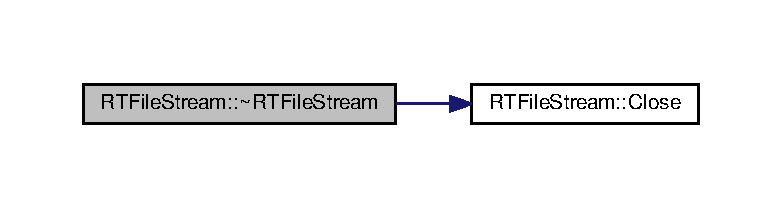
\includegraphics[width=350pt]{classRTFileStream_ad7666167a8f708f4f42cc27df446033b_cgraph}
\end{center}
\end{figure}




\subsection{Member Function Documentation}
\hypertarget{classRTFileStream_acaae552bed709bfeb980b392ce5d7752}{\index{R\-T\-File\-Stream@{R\-T\-File\-Stream}!Close@{Close}}
\index{Close@{Close}!RTFileStream@{R\-T\-File\-Stream}}
\subsubsection[{Close}]{\setlength{\rightskip}{0pt plus 5cm}void R\-T\-File\-Stream\-::\-Close (
\begin{DoxyParamCaption}
{}
\end{DoxyParamCaption}
)\hspace{0.3cm}{\ttfamily [inline]}}}\label{classRTFileStream_acaae552bed709bfeb980b392ce5d7752}
\hypertarget{classRTFileStream_ac6173a0c9e27f20e6be7967973a4c88a}{\index{R\-T\-File\-Stream@{R\-T\-File\-Stream}!Open\-Read@{Open\-Read}}
\index{Open\-Read@{Open\-Read}!RTFileStream@{R\-T\-File\-Stream}}
\subsubsection[{Open\-Read}]{\setlength{\rightskip}{0pt plus 5cm}bool R\-T\-File\-Stream\-::\-Open\-Read (
\begin{DoxyParamCaption}
\item[{const char $\ast$}]{a\-\_\-file\-Name}
\end{DoxyParamCaption}
)\hspace{0.3cm}{\ttfamily [inline]}}}\label{classRTFileStream_ac6173a0c9e27f20e6be7967973a4c88a}
\hypertarget{classRTFileStream_a96b4770d34e8c5188d928ca5e53adb8b}{\index{R\-T\-File\-Stream@{R\-T\-File\-Stream}!Open\-Write@{Open\-Write}}
\index{Open\-Write@{Open\-Write}!RTFileStream@{R\-T\-File\-Stream}}
\subsubsection[{Open\-Write}]{\setlength{\rightskip}{0pt plus 5cm}bool R\-T\-File\-Stream\-::\-Open\-Write (
\begin{DoxyParamCaption}
\item[{const char $\ast$}]{a\-\_\-file\-Name}
\end{DoxyParamCaption}
)\hspace{0.3cm}{\ttfamily [inline]}}}\label{classRTFileStream_a96b4770d34e8c5188d928ca5e53adb8b}
\hypertarget{classRTFileStream_a389780f31ac4853b850fce1ce6ee9df9}{\index{R\-T\-File\-Stream@{R\-T\-File\-Stream}!Read@{Read}}
\index{Read@{Read}!RTFileStream@{R\-T\-File\-Stream}}
\subsubsection[{Read}]{\setlength{\rightskip}{0pt plus 5cm}template$<$typename T\-Y\-P\-E $>$ size\-\_\-t R\-T\-File\-Stream\-::\-Read (
\begin{DoxyParamCaption}
\item[{T\-Y\-P\-E \&}]{a\-\_\-value}
\end{DoxyParamCaption}
)\hspace{0.3cm}{\ttfamily [inline]}}}\label{classRTFileStream_a389780f31ac4853b850fce1ce6ee9df9}
\hypertarget{classRTFileStream_afb034999c38e44e2a80637bfc3b907e5}{\index{R\-T\-File\-Stream@{R\-T\-File\-Stream}!Read\-Array@{Read\-Array}}
\index{Read\-Array@{Read\-Array}!RTFileStream@{R\-T\-File\-Stream}}
\subsubsection[{Read\-Array}]{\setlength{\rightskip}{0pt plus 5cm}template$<$typename T\-Y\-P\-E $>$ size\-\_\-t R\-T\-File\-Stream\-::\-Read\-Array (
\begin{DoxyParamCaption}
\item[{T\-Y\-P\-E $\ast$}]{a\-\_\-array, }
\item[{int}]{a\-\_\-count}
\end{DoxyParamCaption}
)\hspace{0.3cm}{\ttfamily [inline]}}}\label{classRTFileStream_afb034999c38e44e2a80637bfc3b907e5}
\hypertarget{classRTFileStream_a5f58ae8de73d979a992e4d7cfcbd462c}{\index{R\-T\-File\-Stream@{R\-T\-File\-Stream}!Write@{Write}}
\index{Write@{Write}!RTFileStream@{R\-T\-File\-Stream}}
\subsubsection[{Write}]{\setlength{\rightskip}{0pt plus 5cm}template$<$typename T\-Y\-P\-E $>$ size\-\_\-t R\-T\-File\-Stream\-::\-Write (
\begin{DoxyParamCaption}
\item[{const T\-Y\-P\-E \&}]{a\-\_\-value}
\end{DoxyParamCaption}
)\hspace{0.3cm}{\ttfamily [inline]}}}\label{classRTFileStream_a5f58ae8de73d979a992e4d7cfcbd462c}
\hypertarget{classRTFileStream_a7f13b1aa9c3fd6c116c9d482bfc4ae0d}{\index{R\-T\-File\-Stream@{R\-T\-File\-Stream}!Write\-Array@{Write\-Array}}
\index{Write\-Array@{Write\-Array}!RTFileStream@{R\-T\-File\-Stream}}
\subsubsection[{Write\-Array}]{\setlength{\rightskip}{0pt plus 5cm}template$<$typename T\-Y\-P\-E $>$ size\-\_\-t R\-T\-File\-Stream\-::\-Write\-Array (
\begin{DoxyParamCaption}
\item[{const T\-Y\-P\-E $\ast$}]{a\-\_\-array, }
\item[{int}]{a\-\_\-count}
\end{DoxyParamCaption}
)\hspace{0.3cm}{\ttfamily [inline]}}}\label{classRTFileStream_a7f13b1aa9c3fd6c116c9d482bfc4ae0d}


\subsection{Field Documentation}
\hypertarget{classRTFileStream_a835f8a26bae1528a3cfcbc13db62548d}{\index{R\-T\-File\-Stream@{R\-T\-File\-Stream}!m\-\_\-file@{m\-\_\-file}}
\index{m\-\_\-file@{m\-\_\-file}!RTFileStream@{R\-T\-File\-Stream}}
\subsubsection[{m\-\_\-file}]{\setlength{\rightskip}{0pt plus 5cm}F\-I\-L\-E$\ast$ R\-T\-File\-Stream\-::m\-\_\-file\hspace{0.3cm}{\ttfamily [private]}}}\label{classRTFileStream_a835f8a26bae1528a3cfcbc13db62548d}


The documentation for this class was generated from the following file\-:\begin{DoxyCompactItemize}
\item 
\hyperlink{RTree_8h}{R\-Tree.\-h}\end{DoxyCompactItemize}

\hypertarget{classRTree}{\section{R\-Tree$<$ D\-A\-T\-A\-T\-Y\-P\-E, E\-L\-E\-M\-T\-Y\-P\-E, N\-U\-M\-D\-I\-M\-S, E\-L\-E\-M\-T\-Y\-P\-E\-R\-E\-A\-L, T\-M\-A\-X\-N\-O\-D\-E\-S, T\-M\-I\-N\-N\-O\-D\-E\-S $>$ Class Template Reference}
\label{classRTree}\index{R\-Tree$<$ D\-A\-T\-A\-T\-Y\-P\-E, E\-L\-E\-M\-T\-Y\-P\-E, N\-U\-M\-D\-I\-M\-S, E\-L\-E\-M\-T\-Y\-P\-E\-R\-E\-A\-L, T\-M\-A\-X\-N\-O\-D\-E\-S, T\-M\-I\-N\-N\-O\-D\-E\-S $>$@{R\-Tree$<$ D\-A\-T\-A\-T\-Y\-P\-E, E\-L\-E\-M\-T\-Y\-P\-E, N\-U\-M\-D\-I\-M\-S, E\-L\-E\-M\-T\-Y\-P\-E\-R\-E\-A\-L, T\-M\-A\-X\-N\-O\-D\-E\-S, T\-M\-I\-N\-N\-O\-D\-E\-S $>$}}
}


{\ttfamily \#include \char`\"{}R\-Tree.\-h\char`\"{}}



Collaboration diagram for R\-Tree$<$ D\-A\-T\-A\-T\-Y\-P\-E, E\-L\-E\-M\-T\-Y\-P\-E, N\-U\-M\-D\-I\-M\-S, E\-L\-E\-M\-T\-Y\-P\-E\-R\-E\-A\-L, T\-M\-A\-X\-N\-O\-D\-E\-S, T\-M\-I\-N\-N\-O\-D\-E\-S $>$\-:\nopagebreak
\begin{figure}[H]
\begin{center}
\leavevmode
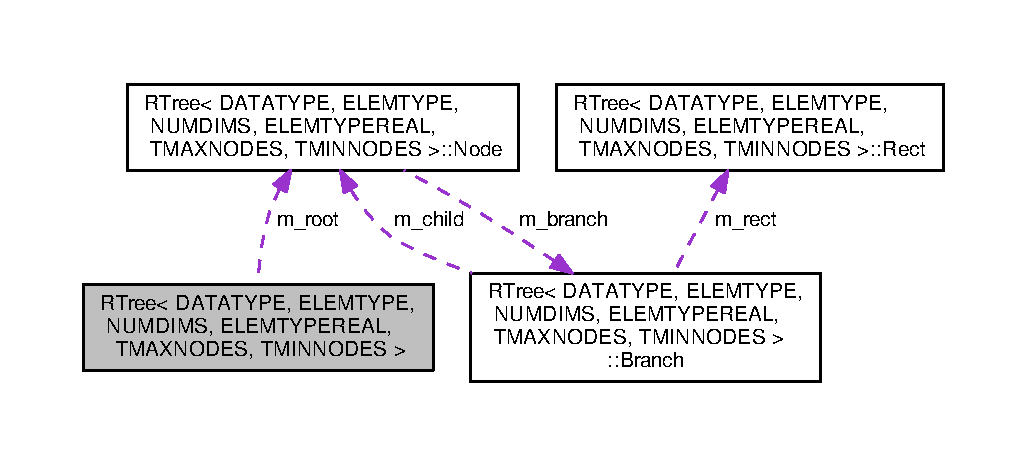
\includegraphics[width=350pt]{classRTree__coll__graph}
\end{center}
\end{figure}
\subsection*{Data Structures}
\begin{DoxyCompactItemize}
\item 
struct \hyperlink{structRTree_1_1Branch}{Branch}
\item 
class \hyperlink{classRTree_1_1Iterator}{Iterator}
\begin{DoxyCompactList}\small\item\em \hyperlink{classRTree_1_1Iterator}{Iterator} is not remove safe. \end{DoxyCompactList}\item 
struct \hyperlink{structRTree_1_1ListNode}{List\-Node}
\begin{DoxyCompactList}\small\item\em A link list of nodes for reinsertion after a delete operation. \end{DoxyCompactList}\item 
struct \hyperlink{structRTree_1_1Node}{Node}
\begin{DoxyCompactList}\small\item\em \hyperlink{structRTree_1_1Node}{Node} for each branch level. \end{DoxyCompactList}\item 
struct \hyperlink{structRTree_1_1PartitionVars}{Partition\-Vars}
\begin{DoxyCompactList}\small\item\em Variables for finding a split partition. \end{DoxyCompactList}\item 
struct \hyperlink{structRTree_1_1Rect}{Rect}
\begin{DoxyCompactList}\small\item\em Minimal bounding rectangle (n-\/dimensional) \end{DoxyCompactList}\end{DoxyCompactItemize}
\subsection*{Public Types}
\begin{DoxyCompactItemize}
\item 
enum \{ \hyperlink{classRTree_afaccb2e611f17ff46b623771ad7043d7ac05afe446df73fa67991e5199453a37f}{M\-A\-X\-N\-O\-D\-E\-S} = T\-M\-A\-X\-N\-O\-D\-E\-S, 
\hyperlink{classRTree_afaccb2e611f17ff46b623771ad7043d7a3be3d8c82fd5bfbd5e5a496e9877d71a}{M\-I\-N\-N\-O\-D\-E\-S} = T\-M\-I\-N\-N\-O\-D\-E\-S
 \}
\item 
typedef bool($\ast$ \hyperlink{classRTree_a989db5f20fcdc26231e8b76be83caee4}{t\-\_\-result\-Callback} )(D\-A\-T\-A\-T\-Y\-P\-E, void $\ast$)
\end{DoxyCompactItemize}
\subsection*{Public Member Functions}
\begin{DoxyCompactItemize}
\item 
\hyperlink{classRTree_a09630e761ba4e88a94a4a80ad40c0700}{R\-Tree} ()
\item 
virtual \hyperlink{classRTree_aad9b714d15f488cd1747cdb619f6b7ee}{$\sim$\-R\-Tree} ()
\item 
void \hyperlink{classRTree_a98d1f0a325921db826b2a2d5a407c9be}{Insert} (const E\-L\-E\-M\-T\-Y\-P\-E a\-\_\-min\mbox{[}N\-U\-M\-D\-I\-M\-S\mbox{]}, const E\-L\-E\-M\-T\-Y\-P\-E a\-\_\-max\mbox{[}N\-U\-M\-D\-I\-M\-S\mbox{]}, const D\-A\-T\-A\-T\-Y\-P\-E \&a\-\_\-data\-Id)
\item 
void \hyperlink{classRTree_a1b4b6b4c73bc47029ba696c49265c043}{Remove} (const E\-L\-E\-M\-T\-Y\-P\-E a\-\_\-min\mbox{[}N\-U\-M\-D\-I\-M\-S\mbox{]}, const E\-L\-E\-M\-T\-Y\-P\-E a\-\_\-max\mbox{[}N\-U\-M\-D\-I\-M\-S\mbox{]}, const D\-A\-T\-A\-T\-Y\-P\-E \&a\-\_\-data\-Id)
\item 
int \hyperlink{classRTree_a3a66726a96bf3c1542d13a2991a25157}{Search} (const E\-L\-E\-M\-T\-Y\-P\-E a\-\_\-min\mbox{[}N\-U\-M\-D\-I\-M\-S\mbox{]}, const E\-L\-E\-M\-T\-Y\-P\-E a\-\_\-max\mbox{[}N\-U\-M\-D\-I\-M\-S\mbox{]}, \hyperlink{classRTree_a989db5f20fcdc26231e8b76be83caee4}{t\-\_\-result\-Callback} a\-\_\-result\-Callback, void $\ast$a\-\_\-context)
\item 
void \hyperlink{classRTree_a396f1031eb2c8224715741fd0b77349d}{Remove\-All} ()
\begin{DoxyCompactList}\small\item\em Remove all entries from tree. \end{DoxyCompactList}\item 
int \hyperlink{classRTree_a813cdf63ce3e3e255821d9ba4bc9e7df}{Count} ()
\begin{DoxyCompactList}\small\item\em Count the data elements in this container. This is slow as no internal counter is maintained. \end{DoxyCompactList}\item 
bool \hyperlink{classRTree_adbd1f87715d22ed75b2b8be738583fc2}{Load} (const char $\ast$a\-\_\-file\-Name)
\begin{DoxyCompactList}\small\item\em Load tree contents from file. \end{DoxyCompactList}\item 
bool \hyperlink{classRTree_ad02dc25a34d9b5b291c8ff3f1b002b09}{Load} (\hyperlink{classRTFileStream}{R\-T\-File\-Stream} \&a\-\_\-stream)
\begin{DoxyCompactList}\small\item\em Load tree contents from stream. \end{DoxyCompactList}\item 
bool \hyperlink{classRTree_a6817692e1e8e416843be1ea628f7a074}{Save} (const char $\ast$a\-\_\-file\-Name)
\begin{DoxyCompactList}\small\item\em Save tree contents to file. \end{DoxyCompactList}\item 
bool \hyperlink{classRTree_a7066ea753180537a3a870c84e4fcefce}{Save} (\hyperlink{classRTFileStream}{R\-T\-File\-Stream} \&a\-\_\-stream)
\begin{DoxyCompactList}\small\item\em Save tree contents to stream. \end{DoxyCompactList}\item 
void \hyperlink{classRTree_acbcbd987b4f6549cd53e373e01b74efa}{Get\-First} (\hyperlink{classRTree_1_1Iterator}{Iterator} \&a\-\_\-it)
\begin{DoxyCompactList}\small\item\em Get 'first' for iteration. \end{DoxyCompactList}\item 
void \hyperlink{classRTree_a41da97d27b44e7d7e852150ced23a610}{Get\-Next} (\hyperlink{classRTree_1_1Iterator}{Iterator} \&a\-\_\-it)
\begin{DoxyCompactList}\small\item\em Get Next for iteration. \end{DoxyCompactList}\item 
bool \hyperlink{classRTree_a8b8c51698e5b8df1e715650a43aad7f4}{Is\-Null} (\hyperlink{classRTree_1_1Iterator}{Iterator} \&a\-\_\-it)
\begin{DoxyCompactList}\small\item\em Is iterator N\-U\-L\-L, or at end? \end{DoxyCompactList}\item 
D\-A\-T\-A\-T\-Y\-P\-E \& \hyperlink{classRTree_aab228fbd816b5e5c93666c37b47635f3}{Get\-At} (\hyperlink{classRTree_1_1Iterator}{Iterator} \&a\-\_\-it)
\begin{DoxyCompactList}\small\item\em Get object at iterator position. \end{DoxyCompactList}\end{DoxyCompactItemize}
\subsection*{Protected Member Functions}
\begin{DoxyCompactItemize}
\item 
\hyperlink{structRTree_1_1Node}{Node} $\ast$ \hyperlink{classRTree_af118b3fc992c88a61fb2e1ebc0c96fc9}{Alloc\-Node} ()
\item 
void \hyperlink{classRTree_a6b5438d9cb74dbfc63f3bfff275f506b}{Free\-Node} (\hyperlink{structRTree_1_1Node}{Node} $\ast$a\-\_\-node)
\item 
void \hyperlink{classRTree_aa24d93770aaa1042136daeabfdb8de3e}{Init\-Node} (\hyperlink{structRTree_1_1Node}{Node} $\ast$a\-\_\-node)
\item 
void \hyperlink{classRTree_aa065e71784e5cac81acd16c07c6abe5e}{Init\-Rect} (\hyperlink{structRTree_1_1Rect}{Rect} $\ast$a\-\_\-rect)
\item 
bool \hyperlink{classRTree_af8e10a4e616414ddf6c0ee40a6c95664}{Insert\-Rect\-Rec} (const \hyperlink{structRTree_1_1Branch}{Branch} \&a\-\_\-branch, \hyperlink{structRTree_1_1Node}{Node} $\ast$a\-\_\-node, \hyperlink{structRTree_1_1Node}{Node} $\ast$$\ast$a\-\_\-new\-Node, int a\-\_\-level)
\item 
bool \hyperlink{classRTree_a0a9b36fceaa83240e41d67b7665f6d3d}{Insert\-Rect} (const \hyperlink{structRTree_1_1Branch}{Branch} \&a\-\_\-branch, \hyperlink{structRTree_1_1Node}{Node} $\ast$$\ast$a\-\_\-root, int a\-\_\-level)
\item 
\hyperlink{structRTree_1_1Rect}{Rect} \hyperlink{classRTree_a19dc96034d7a3230ba877953247457e1}{Node\-Cover} (\hyperlink{structRTree_1_1Node}{Node} $\ast$a\-\_\-node)
\item 
bool \hyperlink{classRTree_a1028d814e1f54328cf58371ea4f9f9bf}{Add\-Branch} (const \hyperlink{structRTree_1_1Branch}{Branch} $\ast$a\-\_\-branch, \hyperlink{structRTree_1_1Node}{Node} $\ast$a\-\_\-node, \hyperlink{structRTree_1_1Node}{Node} $\ast$$\ast$a\-\_\-new\-Node)
\item 
void \hyperlink{classRTree_adcdcac926b2de35cc1f4f07e02b70bf6}{Disconnect\-Branch} (\hyperlink{structRTree_1_1Node}{Node} $\ast$a\-\_\-node, int a\-\_\-index)
\item 
int \hyperlink{classRTree_a142464629cd61c2541d6d0e0cc7d2d80}{Pick\-Branch} (const \hyperlink{structRTree_1_1Rect}{Rect} $\ast$a\-\_\-rect, \hyperlink{structRTree_1_1Node}{Node} $\ast$a\-\_\-node)
\item 
\hyperlink{structRTree_1_1Rect}{Rect} \hyperlink{classRTree_a295ad765615975e4b848592e424a5ca2}{Combine\-Rect} (const \hyperlink{structRTree_1_1Rect}{Rect} $\ast$a\-\_\-rect\-A, const \hyperlink{structRTree_1_1Rect}{Rect} $\ast$a\-\_\-rect\-B)
\item 
void \hyperlink{classRTree_aec268045161713d5225ed8151c5068dd}{Split\-Node} (\hyperlink{structRTree_1_1Node}{Node} $\ast$a\-\_\-node, const \hyperlink{structRTree_1_1Branch}{Branch} $\ast$a\-\_\-branch, \hyperlink{structRTree_1_1Node}{Node} $\ast$$\ast$a\-\_\-new\-Node)
\item 
E\-L\-E\-M\-T\-Y\-P\-E\-R\-E\-A\-L \hyperlink{classRTree_a7958e17fc046e5d648d8e23ffc82e849}{Rect\-Spherical\-Volume} (\hyperlink{structRTree_1_1Rect}{Rect} $\ast$a\-\_\-rect)
\item 
E\-L\-E\-M\-T\-Y\-P\-E\-R\-E\-A\-L \hyperlink{classRTree_af9f63fef551a4c3a42cd915618a9917a}{Rect\-Volume} (\hyperlink{structRTree_1_1Rect}{Rect} $\ast$a\-\_\-rect)
\item 
E\-L\-E\-M\-T\-Y\-P\-E\-R\-E\-A\-L \hyperlink{classRTree_a224ba0af4dcb435dbb016327307d664b}{Calc\-Rect\-Volume} (\hyperlink{structRTree_1_1Rect}{Rect} $\ast$a\-\_\-rect)
\item 
void \hyperlink{classRTree_a3b8fdb0a33793dba49f9870868a95a43}{Get\-Branches} (\hyperlink{structRTree_1_1Node}{Node} $\ast$a\-\_\-node, const \hyperlink{structRTree_1_1Branch}{Branch} $\ast$a\-\_\-branch, \hyperlink{structRTree_1_1PartitionVars}{Partition\-Vars} $\ast$a\-\_\-par\-Vars)
\item 
void \hyperlink{classRTree_a282f6ef6b93f714d8a8eca3c4d587cbd}{Choose\-Partition} (\hyperlink{structRTree_1_1PartitionVars}{Partition\-Vars} $\ast$a\-\_\-par\-Vars, int a\-\_\-min\-Fill)
\item 
void \hyperlink{classRTree_a88e9eef4ad30d4dee0c783df5e6840a0}{Load\-Nodes} (\hyperlink{structRTree_1_1Node}{Node} $\ast$a\-\_\-node\-A, \hyperlink{structRTree_1_1Node}{Node} $\ast$a\-\_\-node\-B, \hyperlink{structRTree_1_1PartitionVars}{Partition\-Vars} $\ast$a\-\_\-par\-Vars)
\item 
void \hyperlink{classRTree_aac207d4389fcca1aa0b72361d84117ec}{Init\-Par\-Vars} (\hyperlink{structRTree_1_1PartitionVars}{Partition\-Vars} $\ast$a\-\_\-par\-Vars, int a\-\_\-max\-Rects, int a\-\_\-min\-Fill)
\item 
void \hyperlink{classRTree_af4232dd5fd978fcce12ce32f9df20f58}{Pick\-Seeds} (\hyperlink{structRTree_1_1PartitionVars}{Partition\-Vars} $\ast$a\-\_\-par\-Vars)
\item 
void \hyperlink{classRTree_a5da8614a152145988f010a0b7ff9cb4d}{Classify} (int a\-\_\-index, int a\-\_\-group, \hyperlink{structRTree_1_1PartitionVars}{Partition\-Vars} $\ast$a\-\_\-par\-Vars)
\item 
bool \hyperlink{classRTree_a64a1092e85775014ce01e1bb6bc8a938}{Remove\-Rect} (\hyperlink{structRTree_1_1Rect}{Rect} $\ast$a\-\_\-rect, const D\-A\-T\-A\-T\-Y\-P\-E \&a\-\_\-id, \hyperlink{structRTree_1_1Node}{Node} $\ast$$\ast$a\-\_\-root)
\item 
bool \hyperlink{classRTree_a519d3084a57b45ed4e4167b382bc977e}{Remove\-Rect\-Rec} (\hyperlink{structRTree_1_1Rect}{Rect} $\ast$a\-\_\-rect, const D\-A\-T\-A\-T\-Y\-P\-E \&a\-\_\-id, \hyperlink{structRTree_1_1Node}{Node} $\ast$a\-\_\-node, \hyperlink{structRTree_1_1ListNode}{List\-Node} $\ast$$\ast$a\-\_\-list\-Node)
\item 
\hyperlink{structRTree_1_1ListNode}{List\-Node} $\ast$ \hyperlink{classRTree_aa688a31e4de0090985045cfabfa42d2d}{Alloc\-List\-Node} ()
\item 
void \hyperlink{classRTree_a0c92660832f03d899608d73b994e95a5}{Free\-List\-Node} (\hyperlink{structRTree_1_1ListNode}{List\-Node} $\ast$a\-\_\-list\-Node)
\item 
bool \hyperlink{classRTree_aa5b369536a94aa8ad9ec3b4f8f68302c}{Overlap} (\hyperlink{structRTree_1_1Rect}{Rect} $\ast$a\-\_\-rect\-A, \hyperlink{structRTree_1_1Rect}{Rect} $\ast$a\-\_\-rect\-B)
\item 
void \hyperlink{classRTree_a5d2b072588eae9e9058224942ae0294f}{Re\-Insert} (\hyperlink{structRTree_1_1Node}{Node} $\ast$a\-\_\-node, \hyperlink{structRTree_1_1ListNode}{List\-Node} $\ast$$\ast$a\-\_\-list\-Node)
\item 
bool \hyperlink{classRTree_a7f84e7f718b4473c435862965033a8d4}{Search} (\hyperlink{structRTree_1_1Node}{Node} $\ast$a\-\_\-node, \hyperlink{structRTree_1_1Rect}{Rect} $\ast$a\-\_\-rect, int \&a\-\_\-found\-Count, \hyperlink{classRTree_a989db5f20fcdc26231e8b76be83caee4}{t\-\_\-result\-Callback} a\-\_\-result\-Callback, void $\ast$a\-\_\-context)
\item 
void \hyperlink{classRTree_a5045d833566114335162fda10d58081d}{Remove\-All\-Rec} (\hyperlink{structRTree_1_1Node}{Node} $\ast$a\-\_\-node)
\item 
void \hyperlink{classRTree_a2508b9d85f5b5f553b313356c05c6e0c}{Reset} ()
\item 
void \hyperlink{classRTree_a22345d494c1d6bf907444f17802bd864}{Count\-Rec} (\hyperlink{structRTree_1_1Node}{Node} $\ast$a\-\_\-node, int \&a\-\_\-count)
\item 
bool \hyperlink{classRTree_a53a8af8a04a9a4a9eb93a6a0792fea95}{Save\-Rec} (\hyperlink{structRTree_1_1Node}{Node} $\ast$a\-\_\-node, \hyperlink{classRTFileStream}{R\-T\-File\-Stream} \&a\-\_\-stream)
\item 
bool \hyperlink{classRTree_aa432ad1d5dfc151c1f8eac388af41968}{Load\-Rec} (\hyperlink{structRTree_1_1Node}{Node} $\ast$a\-\_\-node, \hyperlink{classRTFileStream}{R\-T\-File\-Stream} \&a\-\_\-stream)
\end{DoxyCompactItemize}
\subsection*{Protected Attributes}
\begin{DoxyCompactItemize}
\item 
\hyperlink{structRTree_1_1Node}{Node} $\ast$ \hyperlink{classRTree_a5028f4e28918519bc70cb1f615316582}{m\-\_\-root}
\begin{DoxyCompactList}\small\item\em Root of tree. \end{DoxyCompactList}\item 
E\-L\-E\-M\-T\-Y\-P\-E\-R\-E\-A\-L \hyperlink{classRTree_af26d4beb8ce3a381ee75eabeec4727e3}{m\-\_\-unit\-Sphere\-Volume}
\begin{DoxyCompactList}\small\item\em Unit sphere constant for required number of dimensions. \end{DoxyCompactList}\end{DoxyCompactItemize}


\subsection{Detailed Description}
\subsubsection*{template$<$class D\-A\-T\-A\-T\-Y\-P\-E, class E\-L\-E\-M\-T\-Y\-P\-E, int N\-U\-M\-D\-I\-M\-S, class E\-L\-E\-M\-T\-Y\-P\-E\-R\-E\-A\-L = E\-L\-E\-M\-T\-Y\-P\-E, int T\-M\-A\-X\-N\-O\-D\-E\-S = 8, int T\-M\-I\-N\-N\-O\-D\-E\-S = T\-M\-A\-X\-N\-O\-D\-E\-S / 2$>$class R\-Tree$<$ D\-A\-T\-A\-T\-Y\-P\-E, E\-L\-E\-M\-T\-Y\-P\-E, N\-U\-M\-D\-I\-M\-S, E\-L\-E\-M\-T\-Y\-P\-E\-R\-E\-A\-L, T\-M\-A\-X\-N\-O\-D\-E\-S, T\-M\-I\-N\-N\-O\-D\-E\-S $>$}

Implementation of \hyperlink{classRTree}{R\-Tree}, a multidimensional bounding rectangle tree. Example usage\-: For a 3-\/dimensional tree use R\-Tree$<$\-Object$\ast$, float, 3$>$ my\-Tree;

This modified, templated C++ version by Greg Douglas at Auran (\href{http://www.auran.com}{\tt http\-://www.\-auran.\-com})

D\-A\-T\-A\-T\-Y\-P\-E Referenced data, should be int, void$\ast$, obj$\ast$ etc. no larger than sizeof$<$void$\ast$$>$ and simple type E\-L\-E\-M\-T\-Y\-P\-E Type of element such as int or float N\-U\-M\-D\-I\-M\-S Number of dimensions such as 2 or 3 E\-L\-E\-M\-T\-Y\-P\-E\-R\-E\-A\-L Type of element that allows fractional and large values such as float or double, for use in volume calcs

N\-O\-T\-E\-S\-: Inserting and removing data requires the knowledge of its constant Minimal Bounding Rectangle. This version uses new/delete for nodes, I recommend using a fixed size allocator for efficiency. Instead of using a callback function for returned results, I recommend and efficient pre-\/sized, grow-\/only memory array similar to M\-F\-C C\-Array or S\-T\-L Vector for returning search query result. 

\subsection{Member Typedef Documentation}
\hypertarget{classRTree_a989db5f20fcdc26231e8b76be83caee4}{\index{R\-Tree@{R\-Tree}!t\-\_\-result\-Callback@{t\-\_\-result\-Callback}}
\index{t\-\_\-result\-Callback@{t\-\_\-result\-Callback}!RTree@{R\-Tree}}
\subsubsection[{t\-\_\-result\-Callback}]{\setlength{\rightskip}{0pt plus 5cm}template$<$class D\-A\-T\-A\-T\-Y\-P\-E, class E\-L\-E\-M\-T\-Y\-P\-E, int N\-U\-M\-D\-I\-M\-S, class E\-L\-E\-M\-T\-Y\-P\-E\-R\-E\-A\-L = E\-L\-E\-M\-T\-Y\-P\-E, int T\-M\-A\-X\-N\-O\-D\-E\-S = 8, int T\-M\-I\-N\-N\-O\-D\-E\-S = T\-M\-A\-X\-N\-O\-D\-E\-S / 2$>$ typedef bool($\ast$ {\bf R\-Tree}$<$ D\-A\-T\-A\-T\-Y\-P\-E, E\-L\-E\-M\-T\-Y\-P\-E, N\-U\-M\-D\-I\-M\-S, E\-L\-E\-M\-T\-Y\-P\-E\-R\-E\-A\-L, T\-M\-A\-X\-N\-O\-D\-E\-S, T\-M\-I\-N\-N\-O\-D\-E\-S $>$\-::t\-\_\-result\-Callback)(D\-A\-T\-A\-T\-Y\-P\-E, void $\ast$)}}\label{classRTree_a989db5f20fcdc26231e8b76be83caee4}


\subsection{Member Enumeration Documentation}
\hypertarget{classRTree_afaccb2e611f17ff46b623771ad7043d7}{\subsubsection[{anonymous enum}]{\setlength{\rightskip}{0pt plus 5cm}template$<$class D\-A\-T\-A\-T\-Y\-P\-E, class E\-L\-E\-M\-T\-Y\-P\-E, int N\-U\-M\-D\-I\-M\-S, class E\-L\-E\-M\-T\-Y\-P\-E\-R\-E\-A\-L = E\-L\-E\-M\-T\-Y\-P\-E, int T\-M\-A\-X\-N\-O\-D\-E\-S = 8, int T\-M\-I\-N\-N\-O\-D\-E\-S = T\-M\-A\-X\-N\-O\-D\-E\-S / 2$>$ anonymous enum}}\label{classRTree_afaccb2e611f17ff46b623771ad7043d7}
\begin{Desc}
\item[Enumerator]\par
\begin{description}
\index{M\-A\-X\-N\-O\-D\-E\-S@{M\-A\-X\-N\-O\-D\-E\-S}!R\-Tree@{R\-Tree}}\index{R\-Tree@{R\-Tree}!M\-A\-X\-N\-O\-D\-E\-S@{M\-A\-X\-N\-O\-D\-E\-S}}\item[{\em 
\hypertarget{classRTree_afaccb2e611f17ff46b623771ad7043d7ac05afe446df73fa67991e5199453a37f}{M\-A\-X\-N\-O\-D\-E\-S}\label{classRTree_afaccb2e611f17ff46b623771ad7043d7ac05afe446df73fa67991e5199453a37f}
}]Max elements in node. \index{M\-I\-N\-N\-O\-D\-E\-S@{M\-I\-N\-N\-O\-D\-E\-S}!R\-Tree@{R\-Tree}}\index{R\-Tree@{R\-Tree}!M\-I\-N\-N\-O\-D\-E\-S@{M\-I\-N\-N\-O\-D\-E\-S}}\item[{\em 
\hypertarget{classRTree_afaccb2e611f17ff46b623771ad7043d7a3be3d8c82fd5bfbd5e5a496e9877d71a}{M\-I\-N\-N\-O\-D\-E\-S}\label{classRTree_afaccb2e611f17ff46b623771ad7043d7a3be3d8c82fd5bfbd5e5a496e9877d71a}
}]Min elements in node. \end{description}
\end{Desc}


\subsection{Constructor \& Destructor Documentation}
\hypertarget{classRTree_a09630e761ba4e88a94a4a80ad40c0700}{\index{R\-Tree@{R\-Tree}!R\-Tree@{R\-Tree}}
\index{R\-Tree@{R\-Tree}!RTree@{R\-Tree}}
\subsubsection[{R\-Tree}]{\setlength{\rightskip}{0pt plus 5cm}template$<$class D\-A\-T\-A\-T\-Y\-P\-E, class E\-L\-E\-M\-T\-Y\-P\-E, int N\-U\-M\-D\-I\-M\-S, class E\-L\-E\-M\-T\-Y\-P\-E\-R\-E\-A\-L = E\-L\-E\-M\-T\-Y\-P\-E, int T\-M\-A\-X\-N\-O\-D\-E\-S = 8, int T\-M\-I\-N\-N\-O\-D\-E\-S = T\-M\-A\-X\-N\-O\-D\-E\-S / 2$>$ {\bf R\-Tree}$<$ D\-A\-T\-A\-T\-Y\-P\-E, E\-L\-E\-M\-T\-Y\-P\-E, N\-U\-M\-D\-I\-M\-S, E\-L\-E\-M\-T\-Y\-P\-E\-R\-E\-A\-L, T\-M\-A\-X\-N\-O\-D\-E\-S, T\-M\-I\-N\-N\-O\-D\-E\-S $>$\-::{\bf R\-Tree} (
\begin{DoxyParamCaption}
{}
\end{DoxyParamCaption}
)}}\label{classRTree_a09630e761ba4e88a94a4a80ad40c0700}
\hypertarget{classRTree_aad9b714d15f488cd1747cdb619f6b7ee}{\index{R\-Tree@{R\-Tree}!$\sim$\-R\-Tree@{$\sim$\-R\-Tree}}
\index{$\sim$\-R\-Tree@{$\sim$\-R\-Tree}!RTree@{R\-Tree}}
\subsubsection[{$\sim$\-R\-Tree}]{\setlength{\rightskip}{0pt plus 5cm}template$<$class D\-A\-T\-A\-T\-Y\-P\-E, class E\-L\-E\-M\-T\-Y\-P\-E, int N\-U\-M\-D\-I\-M\-S, class E\-L\-E\-M\-T\-Y\-P\-E\-R\-E\-A\-L = E\-L\-E\-M\-T\-Y\-P\-E, int T\-M\-A\-X\-N\-O\-D\-E\-S = 8, int T\-M\-I\-N\-N\-O\-D\-E\-S = T\-M\-A\-X\-N\-O\-D\-E\-S / 2$>$ virtual {\bf R\-Tree}$<$ D\-A\-T\-A\-T\-Y\-P\-E, E\-L\-E\-M\-T\-Y\-P\-E, N\-U\-M\-D\-I\-M\-S, E\-L\-E\-M\-T\-Y\-P\-E\-R\-E\-A\-L, T\-M\-A\-X\-N\-O\-D\-E\-S, T\-M\-I\-N\-N\-O\-D\-E\-S $>$\-::$\sim${\bf R\-Tree} (
\begin{DoxyParamCaption}
{}
\end{DoxyParamCaption}
)\hspace{0.3cm}{\ttfamily [virtual]}}}\label{classRTree_aad9b714d15f488cd1747cdb619f6b7ee}


\subsection{Member Function Documentation}
\hypertarget{classRTree_a1028d814e1f54328cf58371ea4f9f9bf}{\index{R\-Tree@{R\-Tree}!Add\-Branch@{Add\-Branch}}
\index{Add\-Branch@{Add\-Branch}!RTree@{R\-Tree}}
\subsubsection[{Add\-Branch}]{\setlength{\rightskip}{0pt plus 5cm}template$<$class D\-A\-T\-A\-T\-Y\-P\-E, class E\-L\-E\-M\-T\-Y\-P\-E, int N\-U\-M\-D\-I\-M\-S, class E\-L\-E\-M\-T\-Y\-P\-E\-R\-E\-A\-L = E\-L\-E\-M\-T\-Y\-P\-E, int T\-M\-A\-X\-N\-O\-D\-E\-S = 8, int T\-M\-I\-N\-N\-O\-D\-E\-S = T\-M\-A\-X\-N\-O\-D\-E\-S / 2$>$ bool {\bf R\-Tree}$<$ D\-A\-T\-A\-T\-Y\-P\-E, E\-L\-E\-M\-T\-Y\-P\-E, N\-U\-M\-D\-I\-M\-S, E\-L\-E\-M\-T\-Y\-P\-E\-R\-E\-A\-L, T\-M\-A\-X\-N\-O\-D\-E\-S, T\-M\-I\-N\-N\-O\-D\-E\-S $>$\-::Add\-Branch (
\begin{DoxyParamCaption}
\item[{const {\bf Branch} $\ast$}]{a\-\_\-branch, }
\item[{{\bf Node} $\ast$}]{a\-\_\-node, }
\item[{{\bf Node} $\ast$$\ast$}]{a\-\_\-new\-Node}
\end{DoxyParamCaption}
)\hspace{0.3cm}{\ttfamily [protected]}}}\label{classRTree_a1028d814e1f54328cf58371ea4f9f9bf}
\hypertarget{classRTree_aa688a31e4de0090985045cfabfa42d2d}{\index{R\-Tree@{R\-Tree}!Alloc\-List\-Node@{Alloc\-List\-Node}}
\index{Alloc\-List\-Node@{Alloc\-List\-Node}!RTree@{R\-Tree}}
\subsubsection[{Alloc\-List\-Node}]{\setlength{\rightskip}{0pt plus 5cm}template$<$class D\-A\-T\-A\-T\-Y\-P\-E, class E\-L\-E\-M\-T\-Y\-P\-E, int N\-U\-M\-D\-I\-M\-S, class E\-L\-E\-M\-T\-Y\-P\-E\-R\-E\-A\-L = E\-L\-E\-M\-T\-Y\-P\-E, int T\-M\-A\-X\-N\-O\-D\-E\-S = 8, int T\-M\-I\-N\-N\-O\-D\-E\-S = T\-M\-A\-X\-N\-O\-D\-E\-S / 2$>$ {\bf List\-Node}$\ast$ {\bf R\-Tree}$<$ D\-A\-T\-A\-T\-Y\-P\-E, E\-L\-E\-M\-T\-Y\-P\-E, N\-U\-M\-D\-I\-M\-S, E\-L\-E\-M\-T\-Y\-P\-E\-R\-E\-A\-L, T\-M\-A\-X\-N\-O\-D\-E\-S, T\-M\-I\-N\-N\-O\-D\-E\-S $>$\-::Alloc\-List\-Node (
\begin{DoxyParamCaption}
{}
\end{DoxyParamCaption}
)\hspace{0.3cm}{\ttfamily [protected]}}}\label{classRTree_aa688a31e4de0090985045cfabfa42d2d}
\hypertarget{classRTree_af118b3fc992c88a61fb2e1ebc0c96fc9}{\index{R\-Tree@{R\-Tree}!Alloc\-Node@{Alloc\-Node}}
\index{Alloc\-Node@{Alloc\-Node}!RTree@{R\-Tree}}
\subsubsection[{Alloc\-Node}]{\setlength{\rightskip}{0pt plus 5cm}template$<$class D\-A\-T\-A\-T\-Y\-P\-E, class E\-L\-E\-M\-T\-Y\-P\-E, int N\-U\-M\-D\-I\-M\-S, class E\-L\-E\-M\-T\-Y\-P\-E\-R\-E\-A\-L = E\-L\-E\-M\-T\-Y\-P\-E, int T\-M\-A\-X\-N\-O\-D\-E\-S = 8, int T\-M\-I\-N\-N\-O\-D\-E\-S = T\-M\-A\-X\-N\-O\-D\-E\-S / 2$>$ {\bf Node}$\ast$ {\bf R\-Tree}$<$ D\-A\-T\-A\-T\-Y\-P\-E, E\-L\-E\-M\-T\-Y\-P\-E, N\-U\-M\-D\-I\-M\-S, E\-L\-E\-M\-T\-Y\-P\-E\-R\-E\-A\-L, T\-M\-A\-X\-N\-O\-D\-E\-S, T\-M\-I\-N\-N\-O\-D\-E\-S $>$\-::Alloc\-Node (
\begin{DoxyParamCaption}
{}
\end{DoxyParamCaption}
)\hspace{0.3cm}{\ttfamily [protected]}}}\label{classRTree_af118b3fc992c88a61fb2e1ebc0c96fc9}
\hypertarget{classRTree_a224ba0af4dcb435dbb016327307d664b}{\index{R\-Tree@{R\-Tree}!Calc\-Rect\-Volume@{Calc\-Rect\-Volume}}
\index{Calc\-Rect\-Volume@{Calc\-Rect\-Volume}!RTree@{R\-Tree}}
\subsubsection[{Calc\-Rect\-Volume}]{\setlength{\rightskip}{0pt plus 5cm}template$<$class D\-A\-T\-A\-T\-Y\-P\-E, class E\-L\-E\-M\-T\-Y\-P\-E, int N\-U\-M\-D\-I\-M\-S, class E\-L\-E\-M\-T\-Y\-P\-E\-R\-E\-A\-L = E\-L\-E\-M\-T\-Y\-P\-E, int T\-M\-A\-X\-N\-O\-D\-E\-S = 8, int T\-M\-I\-N\-N\-O\-D\-E\-S = T\-M\-A\-X\-N\-O\-D\-E\-S / 2$>$ E\-L\-E\-M\-T\-Y\-P\-E\-R\-E\-A\-L {\bf R\-Tree}$<$ D\-A\-T\-A\-T\-Y\-P\-E, E\-L\-E\-M\-T\-Y\-P\-E, N\-U\-M\-D\-I\-M\-S, E\-L\-E\-M\-T\-Y\-P\-E\-R\-E\-A\-L, T\-M\-A\-X\-N\-O\-D\-E\-S, T\-M\-I\-N\-N\-O\-D\-E\-S $>$\-::Calc\-Rect\-Volume (
\begin{DoxyParamCaption}
\item[{{\bf Rect} $\ast$}]{a\-\_\-rect}
\end{DoxyParamCaption}
)\hspace{0.3cm}{\ttfamily [protected]}}}\label{classRTree_a224ba0af4dcb435dbb016327307d664b}
\hypertarget{classRTree_a282f6ef6b93f714d8a8eca3c4d587cbd}{\index{R\-Tree@{R\-Tree}!Choose\-Partition@{Choose\-Partition}}
\index{Choose\-Partition@{Choose\-Partition}!RTree@{R\-Tree}}
\subsubsection[{Choose\-Partition}]{\setlength{\rightskip}{0pt plus 5cm}template$<$class D\-A\-T\-A\-T\-Y\-P\-E, class E\-L\-E\-M\-T\-Y\-P\-E, int N\-U\-M\-D\-I\-M\-S, class E\-L\-E\-M\-T\-Y\-P\-E\-R\-E\-A\-L = E\-L\-E\-M\-T\-Y\-P\-E, int T\-M\-A\-X\-N\-O\-D\-E\-S = 8, int T\-M\-I\-N\-N\-O\-D\-E\-S = T\-M\-A\-X\-N\-O\-D\-E\-S / 2$>$ void {\bf R\-Tree}$<$ D\-A\-T\-A\-T\-Y\-P\-E, E\-L\-E\-M\-T\-Y\-P\-E, N\-U\-M\-D\-I\-M\-S, E\-L\-E\-M\-T\-Y\-P\-E\-R\-E\-A\-L, T\-M\-A\-X\-N\-O\-D\-E\-S, T\-M\-I\-N\-N\-O\-D\-E\-S $>$\-::Choose\-Partition (
\begin{DoxyParamCaption}
\item[{{\bf Partition\-Vars} $\ast$}]{a\-\_\-par\-Vars, }
\item[{int}]{a\-\_\-min\-Fill}
\end{DoxyParamCaption}
)\hspace{0.3cm}{\ttfamily [protected]}}}\label{classRTree_a282f6ef6b93f714d8a8eca3c4d587cbd}
\hypertarget{classRTree_a5da8614a152145988f010a0b7ff9cb4d}{\index{R\-Tree@{R\-Tree}!Classify@{Classify}}
\index{Classify@{Classify}!RTree@{R\-Tree}}
\subsubsection[{Classify}]{\setlength{\rightskip}{0pt plus 5cm}template$<$class D\-A\-T\-A\-T\-Y\-P\-E, class E\-L\-E\-M\-T\-Y\-P\-E, int N\-U\-M\-D\-I\-M\-S, class E\-L\-E\-M\-T\-Y\-P\-E\-R\-E\-A\-L = E\-L\-E\-M\-T\-Y\-P\-E, int T\-M\-A\-X\-N\-O\-D\-E\-S = 8, int T\-M\-I\-N\-N\-O\-D\-E\-S = T\-M\-A\-X\-N\-O\-D\-E\-S / 2$>$ void {\bf R\-Tree}$<$ D\-A\-T\-A\-T\-Y\-P\-E, E\-L\-E\-M\-T\-Y\-P\-E, N\-U\-M\-D\-I\-M\-S, E\-L\-E\-M\-T\-Y\-P\-E\-R\-E\-A\-L, T\-M\-A\-X\-N\-O\-D\-E\-S, T\-M\-I\-N\-N\-O\-D\-E\-S $>$\-::Classify (
\begin{DoxyParamCaption}
\item[{int}]{a\-\_\-index, }
\item[{int}]{a\-\_\-group, }
\item[{{\bf Partition\-Vars} $\ast$}]{a\-\_\-par\-Vars}
\end{DoxyParamCaption}
)\hspace{0.3cm}{\ttfamily [protected]}}}\label{classRTree_a5da8614a152145988f010a0b7ff9cb4d}
\hypertarget{classRTree_a295ad765615975e4b848592e424a5ca2}{\index{R\-Tree@{R\-Tree}!Combine\-Rect@{Combine\-Rect}}
\index{Combine\-Rect@{Combine\-Rect}!RTree@{R\-Tree}}
\subsubsection[{Combine\-Rect}]{\setlength{\rightskip}{0pt plus 5cm}template$<$class D\-A\-T\-A\-T\-Y\-P\-E, class E\-L\-E\-M\-T\-Y\-P\-E, int N\-U\-M\-D\-I\-M\-S, class E\-L\-E\-M\-T\-Y\-P\-E\-R\-E\-A\-L = E\-L\-E\-M\-T\-Y\-P\-E, int T\-M\-A\-X\-N\-O\-D\-E\-S = 8, int T\-M\-I\-N\-N\-O\-D\-E\-S = T\-M\-A\-X\-N\-O\-D\-E\-S / 2$>$ {\bf Rect} {\bf R\-Tree}$<$ D\-A\-T\-A\-T\-Y\-P\-E, E\-L\-E\-M\-T\-Y\-P\-E, N\-U\-M\-D\-I\-M\-S, E\-L\-E\-M\-T\-Y\-P\-E\-R\-E\-A\-L, T\-M\-A\-X\-N\-O\-D\-E\-S, T\-M\-I\-N\-N\-O\-D\-E\-S $>$\-::Combine\-Rect (
\begin{DoxyParamCaption}
\item[{const {\bf Rect} $\ast$}]{a\-\_\-rect\-A, }
\item[{const {\bf Rect} $\ast$}]{a\-\_\-rect\-B}
\end{DoxyParamCaption}
)\hspace{0.3cm}{\ttfamily [protected]}}}\label{classRTree_a295ad765615975e4b848592e424a5ca2}
\hypertarget{classRTree_a813cdf63ce3e3e255821d9ba4bc9e7df}{\index{R\-Tree@{R\-Tree}!Count@{Count}}
\index{Count@{Count}!RTree@{R\-Tree}}
\subsubsection[{Count}]{\setlength{\rightskip}{0pt plus 5cm}template$<$class D\-A\-T\-A\-T\-Y\-P\-E, class E\-L\-E\-M\-T\-Y\-P\-E, int N\-U\-M\-D\-I\-M\-S, class E\-L\-E\-M\-T\-Y\-P\-E\-R\-E\-A\-L = E\-L\-E\-M\-T\-Y\-P\-E, int T\-M\-A\-X\-N\-O\-D\-E\-S = 8, int T\-M\-I\-N\-N\-O\-D\-E\-S = T\-M\-A\-X\-N\-O\-D\-E\-S / 2$>$ int {\bf R\-Tree}$<$ D\-A\-T\-A\-T\-Y\-P\-E, E\-L\-E\-M\-T\-Y\-P\-E, N\-U\-M\-D\-I\-M\-S, E\-L\-E\-M\-T\-Y\-P\-E\-R\-E\-A\-L, T\-M\-A\-X\-N\-O\-D\-E\-S, T\-M\-I\-N\-N\-O\-D\-E\-S $>$\-::Count (
\begin{DoxyParamCaption}
{}
\end{DoxyParamCaption}
)}}\label{classRTree_a813cdf63ce3e3e255821d9ba4bc9e7df}


Count the data elements in this container. This is slow as no internal counter is maintained. 

\hypertarget{classRTree_a22345d494c1d6bf907444f17802bd864}{\index{R\-Tree@{R\-Tree}!Count\-Rec@{Count\-Rec}}
\index{Count\-Rec@{Count\-Rec}!RTree@{R\-Tree}}
\subsubsection[{Count\-Rec}]{\setlength{\rightskip}{0pt plus 5cm}template$<$class D\-A\-T\-A\-T\-Y\-P\-E, class E\-L\-E\-M\-T\-Y\-P\-E, int N\-U\-M\-D\-I\-M\-S, class E\-L\-E\-M\-T\-Y\-P\-E\-R\-E\-A\-L = E\-L\-E\-M\-T\-Y\-P\-E, int T\-M\-A\-X\-N\-O\-D\-E\-S = 8, int T\-M\-I\-N\-N\-O\-D\-E\-S = T\-M\-A\-X\-N\-O\-D\-E\-S / 2$>$ void {\bf R\-Tree}$<$ D\-A\-T\-A\-T\-Y\-P\-E, E\-L\-E\-M\-T\-Y\-P\-E, N\-U\-M\-D\-I\-M\-S, E\-L\-E\-M\-T\-Y\-P\-E\-R\-E\-A\-L, T\-M\-A\-X\-N\-O\-D\-E\-S, T\-M\-I\-N\-N\-O\-D\-E\-S $>$\-::Count\-Rec (
\begin{DoxyParamCaption}
\item[{{\bf Node} $\ast$}]{a\-\_\-node, }
\item[{int \&}]{a\-\_\-count}
\end{DoxyParamCaption}
)\hspace{0.3cm}{\ttfamily [protected]}}}\label{classRTree_a22345d494c1d6bf907444f17802bd864}
\hypertarget{classRTree_adcdcac926b2de35cc1f4f07e02b70bf6}{\index{R\-Tree@{R\-Tree}!Disconnect\-Branch@{Disconnect\-Branch}}
\index{Disconnect\-Branch@{Disconnect\-Branch}!RTree@{R\-Tree}}
\subsubsection[{Disconnect\-Branch}]{\setlength{\rightskip}{0pt plus 5cm}template$<$class D\-A\-T\-A\-T\-Y\-P\-E, class E\-L\-E\-M\-T\-Y\-P\-E, int N\-U\-M\-D\-I\-M\-S, class E\-L\-E\-M\-T\-Y\-P\-E\-R\-E\-A\-L = E\-L\-E\-M\-T\-Y\-P\-E, int T\-M\-A\-X\-N\-O\-D\-E\-S = 8, int T\-M\-I\-N\-N\-O\-D\-E\-S = T\-M\-A\-X\-N\-O\-D\-E\-S / 2$>$ void {\bf R\-Tree}$<$ D\-A\-T\-A\-T\-Y\-P\-E, E\-L\-E\-M\-T\-Y\-P\-E, N\-U\-M\-D\-I\-M\-S, E\-L\-E\-M\-T\-Y\-P\-E\-R\-E\-A\-L, T\-M\-A\-X\-N\-O\-D\-E\-S, T\-M\-I\-N\-N\-O\-D\-E\-S $>$\-::Disconnect\-Branch (
\begin{DoxyParamCaption}
\item[{{\bf Node} $\ast$}]{a\-\_\-node, }
\item[{int}]{a\-\_\-index}
\end{DoxyParamCaption}
)\hspace{0.3cm}{\ttfamily [protected]}}}\label{classRTree_adcdcac926b2de35cc1f4f07e02b70bf6}
\hypertarget{classRTree_a0c92660832f03d899608d73b994e95a5}{\index{R\-Tree@{R\-Tree}!Free\-List\-Node@{Free\-List\-Node}}
\index{Free\-List\-Node@{Free\-List\-Node}!RTree@{R\-Tree}}
\subsubsection[{Free\-List\-Node}]{\setlength{\rightskip}{0pt plus 5cm}template$<$class D\-A\-T\-A\-T\-Y\-P\-E, class E\-L\-E\-M\-T\-Y\-P\-E, int N\-U\-M\-D\-I\-M\-S, class E\-L\-E\-M\-T\-Y\-P\-E\-R\-E\-A\-L = E\-L\-E\-M\-T\-Y\-P\-E, int T\-M\-A\-X\-N\-O\-D\-E\-S = 8, int T\-M\-I\-N\-N\-O\-D\-E\-S = T\-M\-A\-X\-N\-O\-D\-E\-S / 2$>$ void {\bf R\-Tree}$<$ D\-A\-T\-A\-T\-Y\-P\-E, E\-L\-E\-M\-T\-Y\-P\-E, N\-U\-M\-D\-I\-M\-S, E\-L\-E\-M\-T\-Y\-P\-E\-R\-E\-A\-L, T\-M\-A\-X\-N\-O\-D\-E\-S, T\-M\-I\-N\-N\-O\-D\-E\-S $>$\-::Free\-List\-Node (
\begin{DoxyParamCaption}
\item[{{\bf List\-Node} $\ast$}]{a\-\_\-list\-Node}
\end{DoxyParamCaption}
)\hspace{0.3cm}{\ttfamily [protected]}}}\label{classRTree_a0c92660832f03d899608d73b994e95a5}
\hypertarget{classRTree_a6b5438d9cb74dbfc63f3bfff275f506b}{\index{R\-Tree@{R\-Tree}!Free\-Node@{Free\-Node}}
\index{Free\-Node@{Free\-Node}!RTree@{R\-Tree}}
\subsubsection[{Free\-Node}]{\setlength{\rightskip}{0pt plus 5cm}template$<$class D\-A\-T\-A\-T\-Y\-P\-E, class E\-L\-E\-M\-T\-Y\-P\-E, int N\-U\-M\-D\-I\-M\-S, class E\-L\-E\-M\-T\-Y\-P\-E\-R\-E\-A\-L = E\-L\-E\-M\-T\-Y\-P\-E, int T\-M\-A\-X\-N\-O\-D\-E\-S = 8, int T\-M\-I\-N\-N\-O\-D\-E\-S = T\-M\-A\-X\-N\-O\-D\-E\-S / 2$>$ void {\bf R\-Tree}$<$ D\-A\-T\-A\-T\-Y\-P\-E, E\-L\-E\-M\-T\-Y\-P\-E, N\-U\-M\-D\-I\-M\-S, E\-L\-E\-M\-T\-Y\-P\-E\-R\-E\-A\-L, T\-M\-A\-X\-N\-O\-D\-E\-S, T\-M\-I\-N\-N\-O\-D\-E\-S $>$\-::Free\-Node (
\begin{DoxyParamCaption}
\item[{{\bf Node} $\ast$}]{a\-\_\-node}
\end{DoxyParamCaption}
)\hspace{0.3cm}{\ttfamily [protected]}}}\label{classRTree_a6b5438d9cb74dbfc63f3bfff275f506b}
\hypertarget{classRTree_aab228fbd816b5e5c93666c37b47635f3}{\index{R\-Tree@{R\-Tree}!Get\-At@{Get\-At}}
\index{Get\-At@{Get\-At}!RTree@{R\-Tree}}
\subsubsection[{Get\-At}]{\setlength{\rightskip}{0pt plus 5cm}template$<$class D\-A\-T\-A\-T\-Y\-P\-E, class E\-L\-E\-M\-T\-Y\-P\-E, int N\-U\-M\-D\-I\-M\-S, class E\-L\-E\-M\-T\-Y\-P\-E\-R\-E\-A\-L = E\-L\-E\-M\-T\-Y\-P\-E, int T\-M\-A\-X\-N\-O\-D\-E\-S = 8, int T\-M\-I\-N\-N\-O\-D\-E\-S = T\-M\-A\-X\-N\-O\-D\-E\-S / 2$>$ D\-A\-T\-A\-T\-Y\-P\-E\& {\bf R\-Tree}$<$ D\-A\-T\-A\-T\-Y\-P\-E, E\-L\-E\-M\-T\-Y\-P\-E, N\-U\-M\-D\-I\-M\-S, E\-L\-E\-M\-T\-Y\-P\-E\-R\-E\-A\-L, T\-M\-A\-X\-N\-O\-D\-E\-S, T\-M\-I\-N\-N\-O\-D\-E\-S $>$\-::Get\-At (
\begin{DoxyParamCaption}
\item[{{\bf Iterator} \&}]{a\-\_\-it}
\end{DoxyParamCaption}
)\hspace{0.3cm}{\ttfamily [inline]}}}\label{classRTree_aab228fbd816b5e5c93666c37b47635f3}


Get object at iterator position. 

\hypertarget{classRTree_a3b8fdb0a33793dba49f9870868a95a43}{\index{R\-Tree@{R\-Tree}!Get\-Branches@{Get\-Branches}}
\index{Get\-Branches@{Get\-Branches}!RTree@{R\-Tree}}
\subsubsection[{Get\-Branches}]{\setlength{\rightskip}{0pt plus 5cm}template$<$class D\-A\-T\-A\-T\-Y\-P\-E, class E\-L\-E\-M\-T\-Y\-P\-E, int N\-U\-M\-D\-I\-M\-S, class E\-L\-E\-M\-T\-Y\-P\-E\-R\-E\-A\-L = E\-L\-E\-M\-T\-Y\-P\-E, int T\-M\-A\-X\-N\-O\-D\-E\-S = 8, int T\-M\-I\-N\-N\-O\-D\-E\-S = T\-M\-A\-X\-N\-O\-D\-E\-S / 2$>$ void {\bf R\-Tree}$<$ D\-A\-T\-A\-T\-Y\-P\-E, E\-L\-E\-M\-T\-Y\-P\-E, N\-U\-M\-D\-I\-M\-S, E\-L\-E\-M\-T\-Y\-P\-E\-R\-E\-A\-L, T\-M\-A\-X\-N\-O\-D\-E\-S, T\-M\-I\-N\-N\-O\-D\-E\-S $>$\-::Get\-Branches (
\begin{DoxyParamCaption}
\item[{{\bf Node} $\ast$}]{a\-\_\-node, }
\item[{const {\bf Branch} $\ast$}]{a\-\_\-branch, }
\item[{{\bf Partition\-Vars} $\ast$}]{a\-\_\-par\-Vars}
\end{DoxyParamCaption}
)\hspace{0.3cm}{\ttfamily [protected]}}}\label{classRTree_a3b8fdb0a33793dba49f9870868a95a43}
\hypertarget{classRTree_acbcbd987b4f6549cd53e373e01b74efa}{\index{R\-Tree@{R\-Tree}!Get\-First@{Get\-First}}
\index{Get\-First@{Get\-First}!RTree@{R\-Tree}}
\subsubsection[{Get\-First}]{\setlength{\rightskip}{0pt plus 5cm}template$<$class D\-A\-T\-A\-T\-Y\-P\-E, class E\-L\-E\-M\-T\-Y\-P\-E, int N\-U\-M\-D\-I\-M\-S, class E\-L\-E\-M\-T\-Y\-P\-E\-R\-E\-A\-L = E\-L\-E\-M\-T\-Y\-P\-E, int T\-M\-A\-X\-N\-O\-D\-E\-S = 8, int T\-M\-I\-N\-N\-O\-D\-E\-S = T\-M\-A\-X\-N\-O\-D\-E\-S / 2$>$ void {\bf R\-Tree}$<$ D\-A\-T\-A\-T\-Y\-P\-E, E\-L\-E\-M\-T\-Y\-P\-E, N\-U\-M\-D\-I\-M\-S, E\-L\-E\-M\-T\-Y\-P\-E\-R\-E\-A\-L, T\-M\-A\-X\-N\-O\-D\-E\-S, T\-M\-I\-N\-N\-O\-D\-E\-S $>$\-::Get\-First (
\begin{DoxyParamCaption}
\item[{{\bf Iterator} \&}]{a\-\_\-it}
\end{DoxyParamCaption}
)\hspace{0.3cm}{\ttfamily [inline]}}}\label{classRTree_acbcbd987b4f6549cd53e373e01b74efa}


Get 'first' for iteration. 

\hypertarget{classRTree_a41da97d27b44e7d7e852150ced23a610}{\index{R\-Tree@{R\-Tree}!Get\-Next@{Get\-Next}}
\index{Get\-Next@{Get\-Next}!RTree@{R\-Tree}}
\subsubsection[{Get\-Next}]{\setlength{\rightskip}{0pt plus 5cm}template$<$class D\-A\-T\-A\-T\-Y\-P\-E, class E\-L\-E\-M\-T\-Y\-P\-E, int N\-U\-M\-D\-I\-M\-S, class E\-L\-E\-M\-T\-Y\-P\-E\-R\-E\-A\-L = E\-L\-E\-M\-T\-Y\-P\-E, int T\-M\-A\-X\-N\-O\-D\-E\-S = 8, int T\-M\-I\-N\-N\-O\-D\-E\-S = T\-M\-A\-X\-N\-O\-D\-E\-S / 2$>$ void {\bf R\-Tree}$<$ D\-A\-T\-A\-T\-Y\-P\-E, E\-L\-E\-M\-T\-Y\-P\-E, N\-U\-M\-D\-I\-M\-S, E\-L\-E\-M\-T\-Y\-P\-E\-R\-E\-A\-L, T\-M\-A\-X\-N\-O\-D\-E\-S, T\-M\-I\-N\-N\-O\-D\-E\-S $>$\-::Get\-Next (
\begin{DoxyParamCaption}
\item[{{\bf Iterator} \&}]{a\-\_\-it}
\end{DoxyParamCaption}
)\hspace{0.3cm}{\ttfamily [inline]}}}\label{classRTree_a41da97d27b44e7d7e852150ced23a610}


Get Next for iteration. 

\hypertarget{classRTree_aa24d93770aaa1042136daeabfdb8de3e}{\index{R\-Tree@{R\-Tree}!Init\-Node@{Init\-Node}}
\index{Init\-Node@{Init\-Node}!RTree@{R\-Tree}}
\subsubsection[{Init\-Node}]{\setlength{\rightskip}{0pt plus 5cm}template$<$class D\-A\-T\-A\-T\-Y\-P\-E, class E\-L\-E\-M\-T\-Y\-P\-E, int N\-U\-M\-D\-I\-M\-S, class E\-L\-E\-M\-T\-Y\-P\-E\-R\-E\-A\-L = E\-L\-E\-M\-T\-Y\-P\-E, int T\-M\-A\-X\-N\-O\-D\-E\-S = 8, int T\-M\-I\-N\-N\-O\-D\-E\-S = T\-M\-A\-X\-N\-O\-D\-E\-S / 2$>$ void {\bf R\-Tree}$<$ D\-A\-T\-A\-T\-Y\-P\-E, E\-L\-E\-M\-T\-Y\-P\-E, N\-U\-M\-D\-I\-M\-S, E\-L\-E\-M\-T\-Y\-P\-E\-R\-E\-A\-L, T\-M\-A\-X\-N\-O\-D\-E\-S, T\-M\-I\-N\-N\-O\-D\-E\-S $>$\-::Init\-Node (
\begin{DoxyParamCaption}
\item[{{\bf Node} $\ast$}]{a\-\_\-node}
\end{DoxyParamCaption}
)\hspace{0.3cm}{\ttfamily [protected]}}}\label{classRTree_aa24d93770aaa1042136daeabfdb8de3e}
\hypertarget{classRTree_aac207d4389fcca1aa0b72361d84117ec}{\index{R\-Tree@{R\-Tree}!Init\-Par\-Vars@{Init\-Par\-Vars}}
\index{Init\-Par\-Vars@{Init\-Par\-Vars}!RTree@{R\-Tree}}
\subsubsection[{Init\-Par\-Vars}]{\setlength{\rightskip}{0pt plus 5cm}template$<$class D\-A\-T\-A\-T\-Y\-P\-E, class E\-L\-E\-M\-T\-Y\-P\-E, int N\-U\-M\-D\-I\-M\-S, class E\-L\-E\-M\-T\-Y\-P\-E\-R\-E\-A\-L = E\-L\-E\-M\-T\-Y\-P\-E, int T\-M\-A\-X\-N\-O\-D\-E\-S = 8, int T\-M\-I\-N\-N\-O\-D\-E\-S = T\-M\-A\-X\-N\-O\-D\-E\-S / 2$>$ void {\bf R\-Tree}$<$ D\-A\-T\-A\-T\-Y\-P\-E, E\-L\-E\-M\-T\-Y\-P\-E, N\-U\-M\-D\-I\-M\-S, E\-L\-E\-M\-T\-Y\-P\-E\-R\-E\-A\-L, T\-M\-A\-X\-N\-O\-D\-E\-S, T\-M\-I\-N\-N\-O\-D\-E\-S $>$\-::Init\-Par\-Vars (
\begin{DoxyParamCaption}
\item[{{\bf Partition\-Vars} $\ast$}]{a\-\_\-par\-Vars, }
\item[{int}]{a\-\_\-max\-Rects, }
\item[{int}]{a\-\_\-min\-Fill}
\end{DoxyParamCaption}
)\hspace{0.3cm}{\ttfamily [protected]}}}\label{classRTree_aac207d4389fcca1aa0b72361d84117ec}
\hypertarget{classRTree_aa065e71784e5cac81acd16c07c6abe5e}{\index{R\-Tree@{R\-Tree}!Init\-Rect@{Init\-Rect}}
\index{Init\-Rect@{Init\-Rect}!RTree@{R\-Tree}}
\subsubsection[{Init\-Rect}]{\setlength{\rightskip}{0pt plus 5cm}template$<$class D\-A\-T\-A\-T\-Y\-P\-E, class E\-L\-E\-M\-T\-Y\-P\-E, int N\-U\-M\-D\-I\-M\-S, class E\-L\-E\-M\-T\-Y\-P\-E\-R\-E\-A\-L = E\-L\-E\-M\-T\-Y\-P\-E, int T\-M\-A\-X\-N\-O\-D\-E\-S = 8, int T\-M\-I\-N\-N\-O\-D\-E\-S = T\-M\-A\-X\-N\-O\-D\-E\-S / 2$>$ void {\bf R\-Tree}$<$ D\-A\-T\-A\-T\-Y\-P\-E, E\-L\-E\-M\-T\-Y\-P\-E, N\-U\-M\-D\-I\-M\-S, E\-L\-E\-M\-T\-Y\-P\-E\-R\-E\-A\-L, T\-M\-A\-X\-N\-O\-D\-E\-S, T\-M\-I\-N\-N\-O\-D\-E\-S $>$\-::Init\-Rect (
\begin{DoxyParamCaption}
\item[{{\bf Rect} $\ast$}]{a\-\_\-rect}
\end{DoxyParamCaption}
)\hspace{0.3cm}{\ttfamily [protected]}}}\label{classRTree_aa065e71784e5cac81acd16c07c6abe5e}
\hypertarget{classRTree_a98d1f0a325921db826b2a2d5a407c9be}{\index{R\-Tree@{R\-Tree}!Insert@{Insert}}
\index{Insert@{Insert}!RTree@{R\-Tree}}
\subsubsection[{Insert}]{\setlength{\rightskip}{0pt plus 5cm}template$<$class D\-A\-T\-A\-T\-Y\-P\-E, class E\-L\-E\-M\-T\-Y\-P\-E, int N\-U\-M\-D\-I\-M\-S, class E\-L\-E\-M\-T\-Y\-P\-E\-R\-E\-A\-L = E\-L\-E\-M\-T\-Y\-P\-E, int T\-M\-A\-X\-N\-O\-D\-E\-S = 8, int T\-M\-I\-N\-N\-O\-D\-E\-S = T\-M\-A\-X\-N\-O\-D\-E\-S / 2$>$ void {\bf R\-Tree}$<$ D\-A\-T\-A\-T\-Y\-P\-E, E\-L\-E\-M\-T\-Y\-P\-E, N\-U\-M\-D\-I\-M\-S, E\-L\-E\-M\-T\-Y\-P\-E\-R\-E\-A\-L, T\-M\-A\-X\-N\-O\-D\-E\-S, T\-M\-I\-N\-N\-O\-D\-E\-S $>$\-::Insert (
\begin{DoxyParamCaption}
\item[{const E\-L\-E\-M\-T\-Y\-P\-E}]{a\-\_\-min\mbox{[}\-N\-U\-M\-D\-I\-M\-S\mbox{]}, }
\item[{const E\-L\-E\-M\-T\-Y\-P\-E}]{a\-\_\-max\mbox{[}\-N\-U\-M\-D\-I\-M\-S\mbox{]}, }
\item[{const D\-A\-T\-A\-T\-Y\-P\-E \&}]{a\-\_\-data\-Id}
\end{DoxyParamCaption}
)}}\label{classRTree_a98d1f0a325921db826b2a2d5a407c9be}
Insert entry 
\begin{DoxyParams}{Parameters}
{\em a\-\_\-min} & Min of bounding rect \\
\hline
{\em a\-\_\-max} & Max of bounding rect \\
\hline
{\em a\-\_\-data\-Id} & Positive Id of data. Maybe zero, but negative numbers not allowed. \\
\hline
\end{DoxyParams}
\hypertarget{classRTree_a0a9b36fceaa83240e41d67b7665f6d3d}{\index{R\-Tree@{R\-Tree}!Insert\-Rect@{Insert\-Rect}}
\index{Insert\-Rect@{Insert\-Rect}!RTree@{R\-Tree}}
\subsubsection[{Insert\-Rect}]{\setlength{\rightskip}{0pt plus 5cm}template$<$class D\-A\-T\-A\-T\-Y\-P\-E, class E\-L\-E\-M\-T\-Y\-P\-E, int N\-U\-M\-D\-I\-M\-S, class E\-L\-E\-M\-T\-Y\-P\-E\-R\-E\-A\-L = E\-L\-E\-M\-T\-Y\-P\-E, int T\-M\-A\-X\-N\-O\-D\-E\-S = 8, int T\-M\-I\-N\-N\-O\-D\-E\-S = T\-M\-A\-X\-N\-O\-D\-E\-S / 2$>$ bool {\bf R\-Tree}$<$ D\-A\-T\-A\-T\-Y\-P\-E, E\-L\-E\-M\-T\-Y\-P\-E, N\-U\-M\-D\-I\-M\-S, E\-L\-E\-M\-T\-Y\-P\-E\-R\-E\-A\-L, T\-M\-A\-X\-N\-O\-D\-E\-S, T\-M\-I\-N\-N\-O\-D\-E\-S $>$\-::Insert\-Rect (
\begin{DoxyParamCaption}
\item[{const {\bf Branch} \&}]{a\-\_\-branch, }
\item[{{\bf Node} $\ast$$\ast$}]{a\-\_\-root, }
\item[{int}]{a\-\_\-level}
\end{DoxyParamCaption}
)\hspace{0.3cm}{\ttfamily [protected]}}}\label{classRTree_a0a9b36fceaa83240e41d67b7665f6d3d}
\hypertarget{classRTree_af8e10a4e616414ddf6c0ee40a6c95664}{\index{R\-Tree@{R\-Tree}!Insert\-Rect\-Rec@{Insert\-Rect\-Rec}}
\index{Insert\-Rect\-Rec@{Insert\-Rect\-Rec}!RTree@{R\-Tree}}
\subsubsection[{Insert\-Rect\-Rec}]{\setlength{\rightskip}{0pt plus 5cm}template$<$class D\-A\-T\-A\-T\-Y\-P\-E, class E\-L\-E\-M\-T\-Y\-P\-E, int N\-U\-M\-D\-I\-M\-S, class E\-L\-E\-M\-T\-Y\-P\-E\-R\-E\-A\-L = E\-L\-E\-M\-T\-Y\-P\-E, int T\-M\-A\-X\-N\-O\-D\-E\-S = 8, int T\-M\-I\-N\-N\-O\-D\-E\-S = T\-M\-A\-X\-N\-O\-D\-E\-S / 2$>$ bool {\bf R\-Tree}$<$ D\-A\-T\-A\-T\-Y\-P\-E, E\-L\-E\-M\-T\-Y\-P\-E, N\-U\-M\-D\-I\-M\-S, E\-L\-E\-M\-T\-Y\-P\-E\-R\-E\-A\-L, T\-M\-A\-X\-N\-O\-D\-E\-S, T\-M\-I\-N\-N\-O\-D\-E\-S $>$\-::Insert\-Rect\-Rec (
\begin{DoxyParamCaption}
\item[{const {\bf Branch} \&}]{a\-\_\-branch, }
\item[{{\bf Node} $\ast$}]{a\-\_\-node, }
\item[{{\bf Node} $\ast$$\ast$}]{a\-\_\-new\-Node, }
\item[{int}]{a\-\_\-level}
\end{DoxyParamCaption}
)\hspace{0.3cm}{\ttfamily [protected]}}}\label{classRTree_af8e10a4e616414ddf6c0ee40a6c95664}
\hypertarget{classRTree_a8b8c51698e5b8df1e715650a43aad7f4}{\index{R\-Tree@{R\-Tree}!Is\-Null@{Is\-Null}}
\index{Is\-Null@{Is\-Null}!RTree@{R\-Tree}}
\subsubsection[{Is\-Null}]{\setlength{\rightskip}{0pt plus 5cm}template$<$class D\-A\-T\-A\-T\-Y\-P\-E, class E\-L\-E\-M\-T\-Y\-P\-E, int N\-U\-M\-D\-I\-M\-S, class E\-L\-E\-M\-T\-Y\-P\-E\-R\-E\-A\-L = E\-L\-E\-M\-T\-Y\-P\-E, int T\-M\-A\-X\-N\-O\-D\-E\-S = 8, int T\-M\-I\-N\-N\-O\-D\-E\-S = T\-M\-A\-X\-N\-O\-D\-E\-S / 2$>$ bool {\bf R\-Tree}$<$ D\-A\-T\-A\-T\-Y\-P\-E, E\-L\-E\-M\-T\-Y\-P\-E, N\-U\-M\-D\-I\-M\-S, E\-L\-E\-M\-T\-Y\-P\-E\-R\-E\-A\-L, T\-M\-A\-X\-N\-O\-D\-E\-S, T\-M\-I\-N\-N\-O\-D\-E\-S $>$\-::Is\-Null (
\begin{DoxyParamCaption}
\item[{{\bf Iterator} \&}]{a\-\_\-it}
\end{DoxyParamCaption}
)\hspace{0.3cm}{\ttfamily [inline]}}}\label{classRTree_a8b8c51698e5b8df1e715650a43aad7f4}


Is iterator N\-U\-L\-L, or at end? 

\hypertarget{classRTree_adbd1f87715d22ed75b2b8be738583fc2}{\index{R\-Tree@{R\-Tree}!Load@{Load}}
\index{Load@{Load}!RTree@{R\-Tree}}
\subsubsection[{Load}]{\setlength{\rightskip}{0pt plus 5cm}template$<$class D\-A\-T\-A\-T\-Y\-P\-E, class E\-L\-E\-M\-T\-Y\-P\-E, int N\-U\-M\-D\-I\-M\-S, class E\-L\-E\-M\-T\-Y\-P\-E\-R\-E\-A\-L = E\-L\-E\-M\-T\-Y\-P\-E, int T\-M\-A\-X\-N\-O\-D\-E\-S = 8, int T\-M\-I\-N\-N\-O\-D\-E\-S = T\-M\-A\-X\-N\-O\-D\-E\-S / 2$>$ bool {\bf R\-Tree}$<$ D\-A\-T\-A\-T\-Y\-P\-E, E\-L\-E\-M\-T\-Y\-P\-E, N\-U\-M\-D\-I\-M\-S, E\-L\-E\-M\-T\-Y\-P\-E\-R\-E\-A\-L, T\-M\-A\-X\-N\-O\-D\-E\-S, T\-M\-I\-N\-N\-O\-D\-E\-S $>$\-::Load (
\begin{DoxyParamCaption}
\item[{const char $\ast$}]{a\-\_\-file\-Name}
\end{DoxyParamCaption}
)}}\label{classRTree_adbd1f87715d22ed75b2b8be738583fc2}


Load tree contents from file. 

\hypertarget{classRTree_ad02dc25a34d9b5b291c8ff3f1b002b09}{\index{R\-Tree@{R\-Tree}!Load@{Load}}
\index{Load@{Load}!RTree@{R\-Tree}}
\subsubsection[{Load}]{\setlength{\rightskip}{0pt plus 5cm}template$<$class D\-A\-T\-A\-T\-Y\-P\-E, class E\-L\-E\-M\-T\-Y\-P\-E, int N\-U\-M\-D\-I\-M\-S, class E\-L\-E\-M\-T\-Y\-P\-E\-R\-E\-A\-L = E\-L\-E\-M\-T\-Y\-P\-E, int T\-M\-A\-X\-N\-O\-D\-E\-S = 8, int T\-M\-I\-N\-N\-O\-D\-E\-S = T\-M\-A\-X\-N\-O\-D\-E\-S / 2$>$ bool {\bf R\-Tree}$<$ D\-A\-T\-A\-T\-Y\-P\-E, E\-L\-E\-M\-T\-Y\-P\-E, N\-U\-M\-D\-I\-M\-S, E\-L\-E\-M\-T\-Y\-P\-E\-R\-E\-A\-L, T\-M\-A\-X\-N\-O\-D\-E\-S, T\-M\-I\-N\-N\-O\-D\-E\-S $>$\-::Load (
\begin{DoxyParamCaption}
\item[{{\bf R\-T\-File\-Stream} \&}]{a\-\_\-stream}
\end{DoxyParamCaption}
)}}\label{classRTree_ad02dc25a34d9b5b291c8ff3f1b002b09}


Load tree contents from stream. 

\hypertarget{classRTree_a88e9eef4ad30d4dee0c783df5e6840a0}{\index{R\-Tree@{R\-Tree}!Load\-Nodes@{Load\-Nodes}}
\index{Load\-Nodes@{Load\-Nodes}!RTree@{R\-Tree}}
\subsubsection[{Load\-Nodes}]{\setlength{\rightskip}{0pt plus 5cm}template$<$class D\-A\-T\-A\-T\-Y\-P\-E, class E\-L\-E\-M\-T\-Y\-P\-E, int N\-U\-M\-D\-I\-M\-S, class E\-L\-E\-M\-T\-Y\-P\-E\-R\-E\-A\-L = E\-L\-E\-M\-T\-Y\-P\-E, int T\-M\-A\-X\-N\-O\-D\-E\-S = 8, int T\-M\-I\-N\-N\-O\-D\-E\-S = T\-M\-A\-X\-N\-O\-D\-E\-S / 2$>$ void {\bf R\-Tree}$<$ D\-A\-T\-A\-T\-Y\-P\-E, E\-L\-E\-M\-T\-Y\-P\-E, N\-U\-M\-D\-I\-M\-S, E\-L\-E\-M\-T\-Y\-P\-E\-R\-E\-A\-L, T\-M\-A\-X\-N\-O\-D\-E\-S, T\-M\-I\-N\-N\-O\-D\-E\-S $>$\-::Load\-Nodes (
\begin{DoxyParamCaption}
\item[{{\bf Node} $\ast$}]{a\-\_\-node\-A, }
\item[{{\bf Node} $\ast$}]{a\-\_\-node\-B, }
\item[{{\bf Partition\-Vars} $\ast$}]{a\-\_\-par\-Vars}
\end{DoxyParamCaption}
)\hspace{0.3cm}{\ttfamily [protected]}}}\label{classRTree_a88e9eef4ad30d4dee0c783df5e6840a0}
\hypertarget{classRTree_aa432ad1d5dfc151c1f8eac388af41968}{\index{R\-Tree@{R\-Tree}!Load\-Rec@{Load\-Rec}}
\index{Load\-Rec@{Load\-Rec}!RTree@{R\-Tree}}
\subsubsection[{Load\-Rec}]{\setlength{\rightskip}{0pt plus 5cm}template$<$class D\-A\-T\-A\-T\-Y\-P\-E, class E\-L\-E\-M\-T\-Y\-P\-E, int N\-U\-M\-D\-I\-M\-S, class E\-L\-E\-M\-T\-Y\-P\-E\-R\-E\-A\-L = E\-L\-E\-M\-T\-Y\-P\-E, int T\-M\-A\-X\-N\-O\-D\-E\-S = 8, int T\-M\-I\-N\-N\-O\-D\-E\-S = T\-M\-A\-X\-N\-O\-D\-E\-S / 2$>$ bool {\bf R\-Tree}$<$ D\-A\-T\-A\-T\-Y\-P\-E, E\-L\-E\-M\-T\-Y\-P\-E, N\-U\-M\-D\-I\-M\-S, E\-L\-E\-M\-T\-Y\-P\-E\-R\-E\-A\-L, T\-M\-A\-X\-N\-O\-D\-E\-S, T\-M\-I\-N\-N\-O\-D\-E\-S $>$\-::Load\-Rec (
\begin{DoxyParamCaption}
\item[{{\bf Node} $\ast$}]{a\-\_\-node, }
\item[{{\bf R\-T\-File\-Stream} \&}]{a\-\_\-stream}
\end{DoxyParamCaption}
)\hspace{0.3cm}{\ttfamily [protected]}}}\label{classRTree_aa432ad1d5dfc151c1f8eac388af41968}
\hypertarget{classRTree_a19dc96034d7a3230ba877953247457e1}{\index{R\-Tree@{R\-Tree}!Node\-Cover@{Node\-Cover}}
\index{Node\-Cover@{Node\-Cover}!RTree@{R\-Tree}}
\subsubsection[{Node\-Cover}]{\setlength{\rightskip}{0pt plus 5cm}template$<$class D\-A\-T\-A\-T\-Y\-P\-E, class E\-L\-E\-M\-T\-Y\-P\-E, int N\-U\-M\-D\-I\-M\-S, class E\-L\-E\-M\-T\-Y\-P\-E\-R\-E\-A\-L = E\-L\-E\-M\-T\-Y\-P\-E, int T\-M\-A\-X\-N\-O\-D\-E\-S = 8, int T\-M\-I\-N\-N\-O\-D\-E\-S = T\-M\-A\-X\-N\-O\-D\-E\-S / 2$>$ {\bf Rect} {\bf R\-Tree}$<$ D\-A\-T\-A\-T\-Y\-P\-E, E\-L\-E\-M\-T\-Y\-P\-E, N\-U\-M\-D\-I\-M\-S, E\-L\-E\-M\-T\-Y\-P\-E\-R\-E\-A\-L, T\-M\-A\-X\-N\-O\-D\-E\-S, T\-M\-I\-N\-N\-O\-D\-E\-S $>$\-::Node\-Cover (
\begin{DoxyParamCaption}
\item[{{\bf Node} $\ast$}]{a\-\_\-node}
\end{DoxyParamCaption}
)\hspace{0.3cm}{\ttfamily [protected]}}}\label{classRTree_a19dc96034d7a3230ba877953247457e1}
\hypertarget{classRTree_aa5b369536a94aa8ad9ec3b4f8f68302c}{\index{R\-Tree@{R\-Tree}!Overlap@{Overlap}}
\index{Overlap@{Overlap}!RTree@{R\-Tree}}
\subsubsection[{Overlap}]{\setlength{\rightskip}{0pt plus 5cm}template$<$class D\-A\-T\-A\-T\-Y\-P\-E, class E\-L\-E\-M\-T\-Y\-P\-E, int N\-U\-M\-D\-I\-M\-S, class E\-L\-E\-M\-T\-Y\-P\-E\-R\-E\-A\-L = E\-L\-E\-M\-T\-Y\-P\-E, int T\-M\-A\-X\-N\-O\-D\-E\-S = 8, int T\-M\-I\-N\-N\-O\-D\-E\-S = T\-M\-A\-X\-N\-O\-D\-E\-S / 2$>$ bool {\bf R\-Tree}$<$ D\-A\-T\-A\-T\-Y\-P\-E, E\-L\-E\-M\-T\-Y\-P\-E, N\-U\-M\-D\-I\-M\-S, E\-L\-E\-M\-T\-Y\-P\-E\-R\-E\-A\-L, T\-M\-A\-X\-N\-O\-D\-E\-S, T\-M\-I\-N\-N\-O\-D\-E\-S $>$\-::Overlap (
\begin{DoxyParamCaption}
\item[{{\bf Rect} $\ast$}]{a\-\_\-rect\-A, }
\item[{{\bf Rect} $\ast$}]{a\-\_\-rect\-B}
\end{DoxyParamCaption}
)\hspace{0.3cm}{\ttfamily [protected]}}}\label{classRTree_aa5b369536a94aa8ad9ec3b4f8f68302c}
\hypertarget{classRTree_a142464629cd61c2541d6d0e0cc7d2d80}{\index{R\-Tree@{R\-Tree}!Pick\-Branch@{Pick\-Branch}}
\index{Pick\-Branch@{Pick\-Branch}!RTree@{R\-Tree}}
\subsubsection[{Pick\-Branch}]{\setlength{\rightskip}{0pt plus 5cm}template$<$class D\-A\-T\-A\-T\-Y\-P\-E, class E\-L\-E\-M\-T\-Y\-P\-E, int N\-U\-M\-D\-I\-M\-S, class E\-L\-E\-M\-T\-Y\-P\-E\-R\-E\-A\-L = E\-L\-E\-M\-T\-Y\-P\-E, int T\-M\-A\-X\-N\-O\-D\-E\-S = 8, int T\-M\-I\-N\-N\-O\-D\-E\-S = T\-M\-A\-X\-N\-O\-D\-E\-S / 2$>$ int {\bf R\-Tree}$<$ D\-A\-T\-A\-T\-Y\-P\-E, E\-L\-E\-M\-T\-Y\-P\-E, N\-U\-M\-D\-I\-M\-S, E\-L\-E\-M\-T\-Y\-P\-E\-R\-E\-A\-L, T\-M\-A\-X\-N\-O\-D\-E\-S, T\-M\-I\-N\-N\-O\-D\-E\-S $>$\-::Pick\-Branch (
\begin{DoxyParamCaption}
\item[{const {\bf Rect} $\ast$}]{a\-\_\-rect, }
\item[{{\bf Node} $\ast$}]{a\-\_\-node}
\end{DoxyParamCaption}
)\hspace{0.3cm}{\ttfamily [protected]}}}\label{classRTree_a142464629cd61c2541d6d0e0cc7d2d80}
\hypertarget{classRTree_af4232dd5fd978fcce12ce32f9df20f58}{\index{R\-Tree@{R\-Tree}!Pick\-Seeds@{Pick\-Seeds}}
\index{Pick\-Seeds@{Pick\-Seeds}!RTree@{R\-Tree}}
\subsubsection[{Pick\-Seeds}]{\setlength{\rightskip}{0pt plus 5cm}template$<$class D\-A\-T\-A\-T\-Y\-P\-E, class E\-L\-E\-M\-T\-Y\-P\-E, int N\-U\-M\-D\-I\-M\-S, class E\-L\-E\-M\-T\-Y\-P\-E\-R\-E\-A\-L = E\-L\-E\-M\-T\-Y\-P\-E, int T\-M\-A\-X\-N\-O\-D\-E\-S = 8, int T\-M\-I\-N\-N\-O\-D\-E\-S = T\-M\-A\-X\-N\-O\-D\-E\-S / 2$>$ void {\bf R\-Tree}$<$ D\-A\-T\-A\-T\-Y\-P\-E, E\-L\-E\-M\-T\-Y\-P\-E, N\-U\-M\-D\-I\-M\-S, E\-L\-E\-M\-T\-Y\-P\-E\-R\-E\-A\-L, T\-M\-A\-X\-N\-O\-D\-E\-S, T\-M\-I\-N\-N\-O\-D\-E\-S $>$\-::Pick\-Seeds (
\begin{DoxyParamCaption}
\item[{{\bf Partition\-Vars} $\ast$}]{a\-\_\-par\-Vars}
\end{DoxyParamCaption}
)\hspace{0.3cm}{\ttfamily [protected]}}}\label{classRTree_af4232dd5fd978fcce12ce32f9df20f58}
\hypertarget{classRTree_a7958e17fc046e5d648d8e23ffc82e849}{\index{R\-Tree@{R\-Tree}!Rect\-Spherical\-Volume@{Rect\-Spherical\-Volume}}
\index{Rect\-Spherical\-Volume@{Rect\-Spherical\-Volume}!RTree@{R\-Tree}}
\subsubsection[{Rect\-Spherical\-Volume}]{\setlength{\rightskip}{0pt plus 5cm}template$<$class D\-A\-T\-A\-T\-Y\-P\-E, class E\-L\-E\-M\-T\-Y\-P\-E, int N\-U\-M\-D\-I\-M\-S, class E\-L\-E\-M\-T\-Y\-P\-E\-R\-E\-A\-L = E\-L\-E\-M\-T\-Y\-P\-E, int T\-M\-A\-X\-N\-O\-D\-E\-S = 8, int T\-M\-I\-N\-N\-O\-D\-E\-S = T\-M\-A\-X\-N\-O\-D\-E\-S / 2$>$ E\-L\-E\-M\-T\-Y\-P\-E\-R\-E\-A\-L {\bf R\-Tree}$<$ D\-A\-T\-A\-T\-Y\-P\-E, E\-L\-E\-M\-T\-Y\-P\-E, N\-U\-M\-D\-I\-M\-S, E\-L\-E\-M\-T\-Y\-P\-E\-R\-E\-A\-L, T\-M\-A\-X\-N\-O\-D\-E\-S, T\-M\-I\-N\-N\-O\-D\-E\-S $>$\-::Rect\-Spherical\-Volume (
\begin{DoxyParamCaption}
\item[{{\bf Rect} $\ast$}]{a\-\_\-rect}
\end{DoxyParamCaption}
)\hspace{0.3cm}{\ttfamily [protected]}}}\label{classRTree_a7958e17fc046e5d648d8e23ffc82e849}
\hypertarget{classRTree_af9f63fef551a4c3a42cd915618a9917a}{\index{R\-Tree@{R\-Tree}!Rect\-Volume@{Rect\-Volume}}
\index{Rect\-Volume@{Rect\-Volume}!RTree@{R\-Tree}}
\subsubsection[{Rect\-Volume}]{\setlength{\rightskip}{0pt plus 5cm}template$<$class D\-A\-T\-A\-T\-Y\-P\-E, class E\-L\-E\-M\-T\-Y\-P\-E, int N\-U\-M\-D\-I\-M\-S, class E\-L\-E\-M\-T\-Y\-P\-E\-R\-E\-A\-L = E\-L\-E\-M\-T\-Y\-P\-E, int T\-M\-A\-X\-N\-O\-D\-E\-S = 8, int T\-M\-I\-N\-N\-O\-D\-E\-S = T\-M\-A\-X\-N\-O\-D\-E\-S / 2$>$ E\-L\-E\-M\-T\-Y\-P\-E\-R\-E\-A\-L {\bf R\-Tree}$<$ D\-A\-T\-A\-T\-Y\-P\-E, E\-L\-E\-M\-T\-Y\-P\-E, N\-U\-M\-D\-I\-M\-S, E\-L\-E\-M\-T\-Y\-P\-E\-R\-E\-A\-L, T\-M\-A\-X\-N\-O\-D\-E\-S, T\-M\-I\-N\-N\-O\-D\-E\-S $>$\-::Rect\-Volume (
\begin{DoxyParamCaption}
\item[{{\bf Rect} $\ast$}]{a\-\_\-rect}
\end{DoxyParamCaption}
)\hspace{0.3cm}{\ttfamily [protected]}}}\label{classRTree_af9f63fef551a4c3a42cd915618a9917a}
\hypertarget{classRTree_a5d2b072588eae9e9058224942ae0294f}{\index{R\-Tree@{R\-Tree}!Re\-Insert@{Re\-Insert}}
\index{Re\-Insert@{Re\-Insert}!RTree@{R\-Tree}}
\subsubsection[{Re\-Insert}]{\setlength{\rightskip}{0pt plus 5cm}template$<$class D\-A\-T\-A\-T\-Y\-P\-E, class E\-L\-E\-M\-T\-Y\-P\-E, int N\-U\-M\-D\-I\-M\-S, class E\-L\-E\-M\-T\-Y\-P\-E\-R\-E\-A\-L = E\-L\-E\-M\-T\-Y\-P\-E, int T\-M\-A\-X\-N\-O\-D\-E\-S = 8, int T\-M\-I\-N\-N\-O\-D\-E\-S = T\-M\-A\-X\-N\-O\-D\-E\-S / 2$>$ void {\bf R\-Tree}$<$ D\-A\-T\-A\-T\-Y\-P\-E, E\-L\-E\-M\-T\-Y\-P\-E, N\-U\-M\-D\-I\-M\-S, E\-L\-E\-M\-T\-Y\-P\-E\-R\-E\-A\-L, T\-M\-A\-X\-N\-O\-D\-E\-S, T\-M\-I\-N\-N\-O\-D\-E\-S $>$\-::Re\-Insert (
\begin{DoxyParamCaption}
\item[{{\bf Node} $\ast$}]{a\-\_\-node, }
\item[{{\bf List\-Node} $\ast$$\ast$}]{a\-\_\-list\-Node}
\end{DoxyParamCaption}
)\hspace{0.3cm}{\ttfamily [protected]}}}\label{classRTree_a5d2b072588eae9e9058224942ae0294f}
\hypertarget{classRTree_a1b4b6b4c73bc47029ba696c49265c043}{\index{R\-Tree@{R\-Tree}!Remove@{Remove}}
\index{Remove@{Remove}!RTree@{R\-Tree}}
\subsubsection[{Remove}]{\setlength{\rightskip}{0pt plus 5cm}template$<$class D\-A\-T\-A\-T\-Y\-P\-E, class E\-L\-E\-M\-T\-Y\-P\-E, int N\-U\-M\-D\-I\-M\-S, class E\-L\-E\-M\-T\-Y\-P\-E\-R\-E\-A\-L = E\-L\-E\-M\-T\-Y\-P\-E, int T\-M\-A\-X\-N\-O\-D\-E\-S = 8, int T\-M\-I\-N\-N\-O\-D\-E\-S = T\-M\-A\-X\-N\-O\-D\-E\-S / 2$>$ void {\bf R\-Tree}$<$ D\-A\-T\-A\-T\-Y\-P\-E, E\-L\-E\-M\-T\-Y\-P\-E, N\-U\-M\-D\-I\-M\-S, E\-L\-E\-M\-T\-Y\-P\-E\-R\-E\-A\-L, T\-M\-A\-X\-N\-O\-D\-E\-S, T\-M\-I\-N\-N\-O\-D\-E\-S $>$\-::Remove (
\begin{DoxyParamCaption}
\item[{const E\-L\-E\-M\-T\-Y\-P\-E}]{a\-\_\-min\mbox{[}\-N\-U\-M\-D\-I\-M\-S\mbox{]}, }
\item[{const E\-L\-E\-M\-T\-Y\-P\-E}]{a\-\_\-max\mbox{[}\-N\-U\-M\-D\-I\-M\-S\mbox{]}, }
\item[{const D\-A\-T\-A\-T\-Y\-P\-E \&}]{a\-\_\-data\-Id}
\end{DoxyParamCaption}
)}}\label{classRTree_a1b4b6b4c73bc47029ba696c49265c043}
Remove entry 
\begin{DoxyParams}{Parameters}
{\em a\-\_\-min} & Min of bounding rect \\
\hline
{\em a\-\_\-max} & Max of bounding rect \\
\hline
{\em a\-\_\-data\-Id} & Positive Id of data. Maybe zero, but negative numbers not allowed. \\
\hline
\end{DoxyParams}
\hypertarget{classRTree_a396f1031eb2c8224715741fd0b77349d}{\index{R\-Tree@{R\-Tree}!Remove\-All@{Remove\-All}}
\index{Remove\-All@{Remove\-All}!RTree@{R\-Tree}}
\subsubsection[{Remove\-All}]{\setlength{\rightskip}{0pt plus 5cm}template$<$class D\-A\-T\-A\-T\-Y\-P\-E, class E\-L\-E\-M\-T\-Y\-P\-E, int N\-U\-M\-D\-I\-M\-S, class E\-L\-E\-M\-T\-Y\-P\-E\-R\-E\-A\-L = E\-L\-E\-M\-T\-Y\-P\-E, int T\-M\-A\-X\-N\-O\-D\-E\-S = 8, int T\-M\-I\-N\-N\-O\-D\-E\-S = T\-M\-A\-X\-N\-O\-D\-E\-S / 2$>$ void {\bf R\-Tree}$<$ D\-A\-T\-A\-T\-Y\-P\-E, E\-L\-E\-M\-T\-Y\-P\-E, N\-U\-M\-D\-I\-M\-S, E\-L\-E\-M\-T\-Y\-P\-E\-R\-E\-A\-L, T\-M\-A\-X\-N\-O\-D\-E\-S, T\-M\-I\-N\-N\-O\-D\-E\-S $>$\-::Remove\-All (
\begin{DoxyParamCaption}
{}
\end{DoxyParamCaption}
)}}\label{classRTree_a396f1031eb2c8224715741fd0b77349d}


Remove all entries from tree. 

\hypertarget{classRTree_a5045d833566114335162fda10d58081d}{\index{R\-Tree@{R\-Tree}!Remove\-All\-Rec@{Remove\-All\-Rec}}
\index{Remove\-All\-Rec@{Remove\-All\-Rec}!RTree@{R\-Tree}}
\subsubsection[{Remove\-All\-Rec}]{\setlength{\rightskip}{0pt plus 5cm}template$<$class D\-A\-T\-A\-T\-Y\-P\-E, class E\-L\-E\-M\-T\-Y\-P\-E, int N\-U\-M\-D\-I\-M\-S, class E\-L\-E\-M\-T\-Y\-P\-E\-R\-E\-A\-L = E\-L\-E\-M\-T\-Y\-P\-E, int T\-M\-A\-X\-N\-O\-D\-E\-S = 8, int T\-M\-I\-N\-N\-O\-D\-E\-S = T\-M\-A\-X\-N\-O\-D\-E\-S / 2$>$ void {\bf R\-Tree}$<$ D\-A\-T\-A\-T\-Y\-P\-E, E\-L\-E\-M\-T\-Y\-P\-E, N\-U\-M\-D\-I\-M\-S, E\-L\-E\-M\-T\-Y\-P\-E\-R\-E\-A\-L, T\-M\-A\-X\-N\-O\-D\-E\-S, T\-M\-I\-N\-N\-O\-D\-E\-S $>$\-::Remove\-All\-Rec (
\begin{DoxyParamCaption}
\item[{{\bf Node} $\ast$}]{a\-\_\-node}
\end{DoxyParamCaption}
)\hspace{0.3cm}{\ttfamily [protected]}}}\label{classRTree_a5045d833566114335162fda10d58081d}
\hypertarget{classRTree_a64a1092e85775014ce01e1bb6bc8a938}{\index{R\-Tree@{R\-Tree}!Remove\-Rect@{Remove\-Rect}}
\index{Remove\-Rect@{Remove\-Rect}!RTree@{R\-Tree}}
\subsubsection[{Remove\-Rect}]{\setlength{\rightskip}{0pt plus 5cm}template$<$class D\-A\-T\-A\-T\-Y\-P\-E, class E\-L\-E\-M\-T\-Y\-P\-E, int N\-U\-M\-D\-I\-M\-S, class E\-L\-E\-M\-T\-Y\-P\-E\-R\-E\-A\-L = E\-L\-E\-M\-T\-Y\-P\-E, int T\-M\-A\-X\-N\-O\-D\-E\-S = 8, int T\-M\-I\-N\-N\-O\-D\-E\-S = T\-M\-A\-X\-N\-O\-D\-E\-S / 2$>$ bool {\bf R\-Tree}$<$ D\-A\-T\-A\-T\-Y\-P\-E, E\-L\-E\-M\-T\-Y\-P\-E, N\-U\-M\-D\-I\-M\-S, E\-L\-E\-M\-T\-Y\-P\-E\-R\-E\-A\-L, T\-M\-A\-X\-N\-O\-D\-E\-S, T\-M\-I\-N\-N\-O\-D\-E\-S $>$\-::Remove\-Rect (
\begin{DoxyParamCaption}
\item[{{\bf Rect} $\ast$}]{a\-\_\-rect, }
\item[{const D\-A\-T\-A\-T\-Y\-P\-E \&}]{a\-\_\-id, }
\item[{{\bf Node} $\ast$$\ast$}]{a\-\_\-root}
\end{DoxyParamCaption}
)\hspace{0.3cm}{\ttfamily [protected]}}}\label{classRTree_a64a1092e85775014ce01e1bb6bc8a938}
\hypertarget{classRTree_a519d3084a57b45ed4e4167b382bc977e}{\index{R\-Tree@{R\-Tree}!Remove\-Rect\-Rec@{Remove\-Rect\-Rec}}
\index{Remove\-Rect\-Rec@{Remove\-Rect\-Rec}!RTree@{R\-Tree}}
\subsubsection[{Remove\-Rect\-Rec}]{\setlength{\rightskip}{0pt plus 5cm}template$<$class D\-A\-T\-A\-T\-Y\-P\-E, class E\-L\-E\-M\-T\-Y\-P\-E, int N\-U\-M\-D\-I\-M\-S, class E\-L\-E\-M\-T\-Y\-P\-E\-R\-E\-A\-L = E\-L\-E\-M\-T\-Y\-P\-E, int T\-M\-A\-X\-N\-O\-D\-E\-S = 8, int T\-M\-I\-N\-N\-O\-D\-E\-S = T\-M\-A\-X\-N\-O\-D\-E\-S / 2$>$ bool {\bf R\-Tree}$<$ D\-A\-T\-A\-T\-Y\-P\-E, E\-L\-E\-M\-T\-Y\-P\-E, N\-U\-M\-D\-I\-M\-S, E\-L\-E\-M\-T\-Y\-P\-E\-R\-E\-A\-L, T\-M\-A\-X\-N\-O\-D\-E\-S, T\-M\-I\-N\-N\-O\-D\-E\-S $>$\-::Remove\-Rect\-Rec (
\begin{DoxyParamCaption}
\item[{{\bf Rect} $\ast$}]{a\-\_\-rect, }
\item[{const D\-A\-T\-A\-T\-Y\-P\-E \&}]{a\-\_\-id, }
\item[{{\bf Node} $\ast$}]{a\-\_\-node, }
\item[{{\bf List\-Node} $\ast$$\ast$}]{a\-\_\-list\-Node}
\end{DoxyParamCaption}
)\hspace{0.3cm}{\ttfamily [protected]}}}\label{classRTree_a519d3084a57b45ed4e4167b382bc977e}
\hypertarget{classRTree_a2508b9d85f5b5f553b313356c05c6e0c}{\index{R\-Tree@{R\-Tree}!Reset@{Reset}}
\index{Reset@{Reset}!RTree@{R\-Tree}}
\subsubsection[{Reset}]{\setlength{\rightskip}{0pt plus 5cm}template$<$class D\-A\-T\-A\-T\-Y\-P\-E, class E\-L\-E\-M\-T\-Y\-P\-E, int N\-U\-M\-D\-I\-M\-S, class E\-L\-E\-M\-T\-Y\-P\-E\-R\-E\-A\-L = E\-L\-E\-M\-T\-Y\-P\-E, int T\-M\-A\-X\-N\-O\-D\-E\-S = 8, int T\-M\-I\-N\-N\-O\-D\-E\-S = T\-M\-A\-X\-N\-O\-D\-E\-S / 2$>$ void {\bf R\-Tree}$<$ D\-A\-T\-A\-T\-Y\-P\-E, E\-L\-E\-M\-T\-Y\-P\-E, N\-U\-M\-D\-I\-M\-S, E\-L\-E\-M\-T\-Y\-P\-E\-R\-E\-A\-L, T\-M\-A\-X\-N\-O\-D\-E\-S, T\-M\-I\-N\-N\-O\-D\-E\-S $>$\-::Reset (
\begin{DoxyParamCaption}
{}
\end{DoxyParamCaption}
)\hspace{0.3cm}{\ttfamily [protected]}}}\label{classRTree_a2508b9d85f5b5f553b313356c05c6e0c}
\hypertarget{classRTree_a6817692e1e8e416843be1ea628f7a074}{\index{R\-Tree@{R\-Tree}!Save@{Save}}
\index{Save@{Save}!RTree@{R\-Tree}}
\subsubsection[{Save}]{\setlength{\rightskip}{0pt plus 5cm}template$<$class D\-A\-T\-A\-T\-Y\-P\-E, class E\-L\-E\-M\-T\-Y\-P\-E, int N\-U\-M\-D\-I\-M\-S, class E\-L\-E\-M\-T\-Y\-P\-E\-R\-E\-A\-L = E\-L\-E\-M\-T\-Y\-P\-E, int T\-M\-A\-X\-N\-O\-D\-E\-S = 8, int T\-M\-I\-N\-N\-O\-D\-E\-S = T\-M\-A\-X\-N\-O\-D\-E\-S / 2$>$ bool {\bf R\-Tree}$<$ D\-A\-T\-A\-T\-Y\-P\-E, E\-L\-E\-M\-T\-Y\-P\-E, N\-U\-M\-D\-I\-M\-S, E\-L\-E\-M\-T\-Y\-P\-E\-R\-E\-A\-L, T\-M\-A\-X\-N\-O\-D\-E\-S, T\-M\-I\-N\-N\-O\-D\-E\-S $>$\-::Save (
\begin{DoxyParamCaption}
\item[{const char $\ast$}]{a\-\_\-file\-Name}
\end{DoxyParamCaption}
)}}\label{classRTree_a6817692e1e8e416843be1ea628f7a074}


Save tree contents to file. 

\hypertarget{classRTree_a7066ea753180537a3a870c84e4fcefce}{\index{R\-Tree@{R\-Tree}!Save@{Save}}
\index{Save@{Save}!RTree@{R\-Tree}}
\subsubsection[{Save}]{\setlength{\rightskip}{0pt plus 5cm}template$<$class D\-A\-T\-A\-T\-Y\-P\-E, class E\-L\-E\-M\-T\-Y\-P\-E, int N\-U\-M\-D\-I\-M\-S, class E\-L\-E\-M\-T\-Y\-P\-E\-R\-E\-A\-L = E\-L\-E\-M\-T\-Y\-P\-E, int T\-M\-A\-X\-N\-O\-D\-E\-S = 8, int T\-M\-I\-N\-N\-O\-D\-E\-S = T\-M\-A\-X\-N\-O\-D\-E\-S / 2$>$ bool {\bf R\-Tree}$<$ D\-A\-T\-A\-T\-Y\-P\-E, E\-L\-E\-M\-T\-Y\-P\-E, N\-U\-M\-D\-I\-M\-S, E\-L\-E\-M\-T\-Y\-P\-E\-R\-E\-A\-L, T\-M\-A\-X\-N\-O\-D\-E\-S, T\-M\-I\-N\-N\-O\-D\-E\-S $>$\-::Save (
\begin{DoxyParamCaption}
\item[{{\bf R\-T\-File\-Stream} \&}]{a\-\_\-stream}
\end{DoxyParamCaption}
)}}\label{classRTree_a7066ea753180537a3a870c84e4fcefce}


Save tree contents to stream. 

\hypertarget{classRTree_a53a8af8a04a9a4a9eb93a6a0792fea95}{\index{R\-Tree@{R\-Tree}!Save\-Rec@{Save\-Rec}}
\index{Save\-Rec@{Save\-Rec}!RTree@{R\-Tree}}
\subsubsection[{Save\-Rec}]{\setlength{\rightskip}{0pt plus 5cm}template$<$class D\-A\-T\-A\-T\-Y\-P\-E, class E\-L\-E\-M\-T\-Y\-P\-E, int N\-U\-M\-D\-I\-M\-S, class E\-L\-E\-M\-T\-Y\-P\-E\-R\-E\-A\-L = E\-L\-E\-M\-T\-Y\-P\-E, int T\-M\-A\-X\-N\-O\-D\-E\-S = 8, int T\-M\-I\-N\-N\-O\-D\-E\-S = T\-M\-A\-X\-N\-O\-D\-E\-S / 2$>$ bool {\bf R\-Tree}$<$ D\-A\-T\-A\-T\-Y\-P\-E, E\-L\-E\-M\-T\-Y\-P\-E, N\-U\-M\-D\-I\-M\-S, E\-L\-E\-M\-T\-Y\-P\-E\-R\-E\-A\-L, T\-M\-A\-X\-N\-O\-D\-E\-S, T\-M\-I\-N\-N\-O\-D\-E\-S $>$\-::Save\-Rec (
\begin{DoxyParamCaption}
\item[{{\bf Node} $\ast$}]{a\-\_\-node, }
\item[{{\bf R\-T\-File\-Stream} \&}]{a\-\_\-stream}
\end{DoxyParamCaption}
)\hspace{0.3cm}{\ttfamily [protected]}}}\label{classRTree_a53a8af8a04a9a4a9eb93a6a0792fea95}
\hypertarget{classRTree_a3a66726a96bf3c1542d13a2991a25157}{\index{R\-Tree@{R\-Tree}!Search@{Search}}
\index{Search@{Search}!RTree@{R\-Tree}}
\subsubsection[{Search}]{\setlength{\rightskip}{0pt plus 5cm}template$<$class D\-A\-T\-A\-T\-Y\-P\-E, class E\-L\-E\-M\-T\-Y\-P\-E, int N\-U\-M\-D\-I\-M\-S, class E\-L\-E\-M\-T\-Y\-P\-E\-R\-E\-A\-L = E\-L\-E\-M\-T\-Y\-P\-E, int T\-M\-A\-X\-N\-O\-D\-E\-S = 8, int T\-M\-I\-N\-N\-O\-D\-E\-S = T\-M\-A\-X\-N\-O\-D\-E\-S / 2$>$ int {\bf R\-Tree}$<$ D\-A\-T\-A\-T\-Y\-P\-E, E\-L\-E\-M\-T\-Y\-P\-E, N\-U\-M\-D\-I\-M\-S, E\-L\-E\-M\-T\-Y\-P\-E\-R\-E\-A\-L, T\-M\-A\-X\-N\-O\-D\-E\-S, T\-M\-I\-N\-N\-O\-D\-E\-S $>$\-::Search (
\begin{DoxyParamCaption}
\item[{const E\-L\-E\-M\-T\-Y\-P\-E}]{a\-\_\-min\mbox{[}\-N\-U\-M\-D\-I\-M\-S\mbox{]}, }
\item[{const E\-L\-E\-M\-T\-Y\-P\-E}]{a\-\_\-max\mbox{[}\-N\-U\-M\-D\-I\-M\-S\mbox{]}, }
\item[{{\bf t\-\_\-result\-Callback}}]{a\-\_\-result\-Callback, }
\item[{void $\ast$}]{a\-\_\-context}
\end{DoxyParamCaption}
)}}\label{classRTree_a3a66726a96bf3c1542d13a2991a25157}
Find all within search rectangle 
\begin{DoxyParams}{Parameters}
{\em a\-\_\-min} & Min of search bounding rect \\
\hline
{\em a\-\_\-max} & Max of search bounding rect \\
\hline
{\em a\-\_\-search\-Result} & Search result array. Caller should set grow size. Function will reset, not append to array. \\
\hline
{\em a\-\_\-result\-Callback} & Callback function to return result. Callback should return 'true' to continue searching \\
\hline
{\em a\-\_\-context} & User context to pass as parameter to a\-\_\-result\-Callback \\
\hline
\end{DoxyParams}
\begin{DoxyReturn}{Returns}
Returns the number of entries found 
\end{DoxyReturn}
\hypertarget{classRTree_a7f84e7f718b4473c435862965033a8d4}{\index{R\-Tree@{R\-Tree}!Search@{Search}}
\index{Search@{Search}!RTree@{R\-Tree}}
\subsubsection[{Search}]{\setlength{\rightskip}{0pt plus 5cm}template$<$class D\-A\-T\-A\-T\-Y\-P\-E, class E\-L\-E\-M\-T\-Y\-P\-E, int N\-U\-M\-D\-I\-M\-S, class E\-L\-E\-M\-T\-Y\-P\-E\-R\-E\-A\-L = E\-L\-E\-M\-T\-Y\-P\-E, int T\-M\-A\-X\-N\-O\-D\-E\-S = 8, int T\-M\-I\-N\-N\-O\-D\-E\-S = T\-M\-A\-X\-N\-O\-D\-E\-S / 2$>$ bool {\bf R\-Tree}$<$ D\-A\-T\-A\-T\-Y\-P\-E, E\-L\-E\-M\-T\-Y\-P\-E, N\-U\-M\-D\-I\-M\-S, E\-L\-E\-M\-T\-Y\-P\-E\-R\-E\-A\-L, T\-M\-A\-X\-N\-O\-D\-E\-S, T\-M\-I\-N\-N\-O\-D\-E\-S $>$\-::Search (
\begin{DoxyParamCaption}
\item[{{\bf Node} $\ast$}]{a\-\_\-node, }
\item[{{\bf Rect} $\ast$}]{a\-\_\-rect, }
\item[{int \&}]{a\-\_\-found\-Count, }
\item[{{\bf t\-\_\-result\-Callback}}]{a\-\_\-result\-Callback, }
\item[{void $\ast$}]{a\-\_\-context}
\end{DoxyParamCaption}
)\hspace{0.3cm}{\ttfamily [protected]}}}\label{classRTree_a7f84e7f718b4473c435862965033a8d4}
\hypertarget{classRTree_aec268045161713d5225ed8151c5068dd}{\index{R\-Tree@{R\-Tree}!Split\-Node@{Split\-Node}}
\index{Split\-Node@{Split\-Node}!RTree@{R\-Tree}}
\subsubsection[{Split\-Node}]{\setlength{\rightskip}{0pt plus 5cm}template$<$class D\-A\-T\-A\-T\-Y\-P\-E, class E\-L\-E\-M\-T\-Y\-P\-E, int N\-U\-M\-D\-I\-M\-S, class E\-L\-E\-M\-T\-Y\-P\-E\-R\-E\-A\-L = E\-L\-E\-M\-T\-Y\-P\-E, int T\-M\-A\-X\-N\-O\-D\-E\-S = 8, int T\-M\-I\-N\-N\-O\-D\-E\-S = T\-M\-A\-X\-N\-O\-D\-E\-S / 2$>$ void {\bf R\-Tree}$<$ D\-A\-T\-A\-T\-Y\-P\-E, E\-L\-E\-M\-T\-Y\-P\-E, N\-U\-M\-D\-I\-M\-S, E\-L\-E\-M\-T\-Y\-P\-E\-R\-E\-A\-L, T\-M\-A\-X\-N\-O\-D\-E\-S, T\-M\-I\-N\-N\-O\-D\-E\-S $>$\-::Split\-Node (
\begin{DoxyParamCaption}
\item[{{\bf Node} $\ast$}]{a\-\_\-node, }
\item[{const {\bf Branch} $\ast$}]{a\-\_\-branch, }
\item[{{\bf Node} $\ast$$\ast$}]{a\-\_\-new\-Node}
\end{DoxyParamCaption}
)\hspace{0.3cm}{\ttfamily [protected]}}}\label{classRTree_aec268045161713d5225ed8151c5068dd}


\subsection{Field Documentation}
\hypertarget{classRTree_a5028f4e28918519bc70cb1f615316582}{\index{R\-Tree@{R\-Tree}!m\-\_\-root@{m\-\_\-root}}
\index{m\-\_\-root@{m\-\_\-root}!RTree@{R\-Tree}}
\subsubsection[{m\-\_\-root}]{\setlength{\rightskip}{0pt plus 5cm}template$<$class D\-A\-T\-A\-T\-Y\-P\-E, class E\-L\-E\-M\-T\-Y\-P\-E, int N\-U\-M\-D\-I\-M\-S, class E\-L\-E\-M\-T\-Y\-P\-E\-R\-E\-A\-L = E\-L\-E\-M\-T\-Y\-P\-E, int T\-M\-A\-X\-N\-O\-D\-E\-S = 8, int T\-M\-I\-N\-N\-O\-D\-E\-S = T\-M\-A\-X\-N\-O\-D\-E\-S / 2$>$ {\bf Node}$\ast$ {\bf R\-Tree}$<$ D\-A\-T\-A\-T\-Y\-P\-E, E\-L\-E\-M\-T\-Y\-P\-E, N\-U\-M\-D\-I\-M\-S, E\-L\-E\-M\-T\-Y\-P\-E\-R\-E\-A\-L, T\-M\-A\-X\-N\-O\-D\-E\-S, T\-M\-I\-N\-N\-O\-D\-E\-S $>$\-::m\-\_\-root\hspace{0.3cm}{\ttfamily [protected]}}}\label{classRTree_a5028f4e28918519bc70cb1f615316582}


Root of tree. 

\hypertarget{classRTree_af26d4beb8ce3a381ee75eabeec4727e3}{\index{R\-Tree@{R\-Tree}!m\-\_\-unit\-Sphere\-Volume@{m\-\_\-unit\-Sphere\-Volume}}
\index{m\-\_\-unit\-Sphere\-Volume@{m\-\_\-unit\-Sphere\-Volume}!RTree@{R\-Tree}}
\subsubsection[{m\-\_\-unit\-Sphere\-Volume}]{\setlength{\rightskip}{0pt plus 5cm}template$<$class D\-A\-T\-A\-T\-Y\-P\-E, class E\-L\-E\-M\-T\-Y\-P\-E, int N\-U\-M\-D\-I\-M\-S, class E\-L\-E\-M\-T\-Y\-P\-E\-R\-E\-A\-L = E\-L\-E\-M\-T\-Y\-P\-E, int T\-M\-A\-X\-N\-O\-D\-E\-S = 8, int T\-M\-I\-N\-N\-O\-D\-E\-S = T\-M\-A\-X\-N\-O\-D\-E\-S / 2$>$ E\-L\-E\-M\-T\-Y\-P\-E\-R\-E\-A\-L {\bf R\-Tree}$<$ D\-A\-T\-A\-T\-Y\-P\-E, E\-L\-E\-M\-T\-Y\-P\-E, N\-U\-M\-D\-I\-M\-S, E\-L\-E\-M\-T\-Y\-P\-E\-R\-E\-A\-L, T\-M\-A\-X\-N\-O\-D\-E\-S, T\-M\-I\-N\-N\-O\-D\-E\-S $>$\-::m\-\_\-unit\-Sphere\-Volume\hspace{0.3cm}{\ttfamily [protected]}}}\label{classRTree_af26d4beb8ce3a381ee75eabeec4727e3}


Unit sphere constant for required number of dimensions. 



The documentation for this class was generated from the following file\-:\begin{DoxyCompactItemize}
\item 
\hyperlink{RTree_8h}{R\-Tree.\-h}\end{DoxyCompactItemize}

\hypertarget{structschedInfo}{\section{sched\-Info Struct Reference}
\label{structschedInfo}\index{sched\-Info@{sched\-Info}}
}


{\ttfamily \#include \char`\"{}structs.\-h\char`\"{}}

\subsection*{Data Fields}
\begin{DoxyCompactItemize}
\item 
bool \hyperlink{structschedInfo_a2baf2f0b93992d3a3302a0107ce68f40}{cluster\-Scratch}
\item 
bool \hyperlink{structschedInfo_a030529daa6752db7ef2302d10c9d3d03}{status}
\end{DoxyCompactItemize}


\subsection{Field Documentation}
\hypertarget{structschedInfo_a2baf2f0b93992d3a3302a0107ce68f40}{\index{sched\-Info@{sched\-Info}!cluster\-Scratch@{cluster\-Scratch}}
\index{cluster\-Scratch@{cluster\-Scratch}!schedInfo@{sched\-Info}}
\subsubsection[{cluster\-Scratch}]{\setlength{\rightskip}{0pt plus 5cm}bool sched\-Info\-::cluster\-Scratch}}\label{structschedInfo_a2baf2f0b93992d3a3302a0107ce68f40}
\hypertarget{structschedInfo_a030529daa6752db7ef2302d10c9d3d03}{\index{sched\-Info@{sched\-Info}!status@{status}}
\index{status@{status}!schedInfo@{sched\-Info}}
\subsubsection[{status}]{\setlength{\rightskip}{0pt plus 5cm}bool sched\-Info\-::status}}\label{structschedInfo_a030529daa6752db7ef2302d10c9d3d03}


The documentation for this struct was generated from the following file\-:\begin{DoxyCompactItemize}
\item 
\hyperlink{structs_8h}{structs.\-h}\end{DoxyCompactItemize}

\hypertarget{classSchedule}{\section{Schedule Class Reference}
\label{classSchedule}\index{Schedule@{Schedule}}
}


{\ttfamily \#include \char`\"{}schedule.\-h\char`\"{}}



Collaboration diagram for Schedule\-:\nopagebreak
\begin{figure}[H]
\begin{center}
\leavevmode
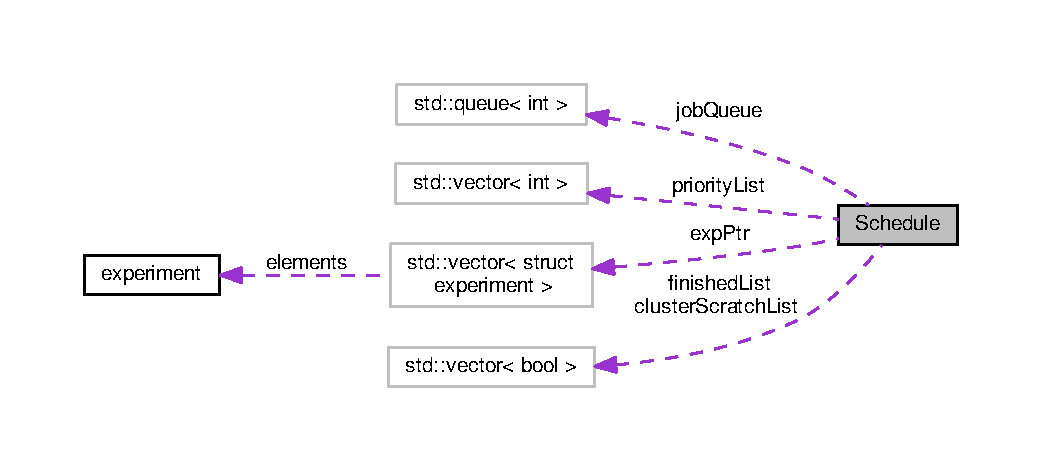
\includegraphics[width=350pt]{classSchedule__coll__graph}
\end{center}
\end{figure}
\subsection*{Public Member Functions}
\begin{DoxyCompactItemize}
\item 
\hyperlink{classSchedule_a5e92f7e6f259168a8634d60d33cd65ed}{Schedule} (vector$<$ struct \hyperlink{structexperiment}{experiment} $>$ $\ast$experiment\-List)
\item 
bool \hyperlink{classSchedule_a2f1dfef54409f093d3900169af84b850}{determine\-Reuse} (int in\-Exper\-I\-D, int $\ast$out\-I\-D\-Reuse, int $\ast$out\-Instance\-Cluster)
\end{DoxyCompactItemize}
\subsection*{Data Fields}
\begin{DoxyCompactItemize}
\item 
std\-::vector$<$ bool $>$ \hyperlink{classSchedule_a0e3d2c52318e5c7060c9fa9ea4e9956b}{finished\-List}
\item 
std\-::vector$<$ struct \hyperlink{structexperiment}{experiment} $>$ $\ast$ \hyperlink{classSchedule_a6be64e3a9e572d346e11481b49d55b7f}{exp\-Ptr}
\end{DoxyCompactItemize}
\subsection*{Private Member Functions}
\begin{DoxyCompactItemize}
\item 
bool \hyperlink{classSchedule_ac301aeb664a5c22bdd0d91aa794d5f7d}{sched\-Greedy} (int $\ast$out\-I\-D, int $\ast$out\-Instance\-Cluster)
\end{DoxyCompactItemize}
\subsection*{Private Attributes}
\begin{DoxyCompactItemize}
\item 
std\-::vector$<$ int $>$ \hyperlink{classSchedule_a3bb97864bd4c176f2c55180671abd0a5}{priority\-List}
\item 
std\-::vector$<$ bool $>$ \hyperlink{classSchedule_a2077242582962c5100fd8d5b086398cb}{cluster\-Scratch\-List}
\item 
std\-::queue$<$ int $>$ \hyperlink{classSchedule_a5ee0c3a418d3d356c972f09ba4bd1513}{job\-Queue}
\end{DoxyCompactItemize}


\subsection{Constructor \& Destructor Documentation}
\hypertarget{classSchedule_a5e92f7e6f259168a8634d60d33cd65ed}{\index{Schedule@{Schedule}!Schedule@{Schedule}}
\index{Schedule@{Schedule}!Schedule@{Schedule}}
\subsubsection[{Schedule}]{\setlength{\rightskip}{0pt plus 5cm}Schedule\-::\-Schedule (
\begin{DoxyParamCaption}
\item[{vector$<$ struct {\bf experiment} $>$ $\ast$}]{experiment\-List}
\end{DoxyParamCaption}
)}}\label{classSchedule_a5e92f7e6f259168a8634d60d33cd65ed}
\hyperlink{classSchedule}{Schedule} constructor 

\subsection{Member Function Documentation}
\hypertarget{classSchedule_a2f1dfef54409f093d3900169af84b850}{\index{Schedule@{Schedule}!determine\-Reuse@{determine\-Reuse}}
\index{determine\-Reuse@{determine\-Reuse}!Schedule@{Schedule}}
\subsubsection[{determine\-Reuse}]{\setlength{\rightskip}{0pt plus 5cm}bool Schedule\-::determine\-Reuse (
\begin{DoxyParamCaption}
\item[{int}]{in\-Exper\-I\-D, }
\item[{int $\ast$}]{out\-I\-D\-Reuse, }
\item[{int $\ast$}]{out\-Instance\-Cluster}
\end{DoxyParamCaption}
)}}\label{classSchedule_a2f1dfef54409f093d3900169af84b850}
Determines if the variant should be clustered from scratch or not If reusing data, then it uses the completed out\-I\-D\-Reuse, and clusters variant out\-Instance\-Cluster 

Here is the call graph for this function\-:\nopagebreak
\begin{figure}[H]
\begin{center}
\leavevmode
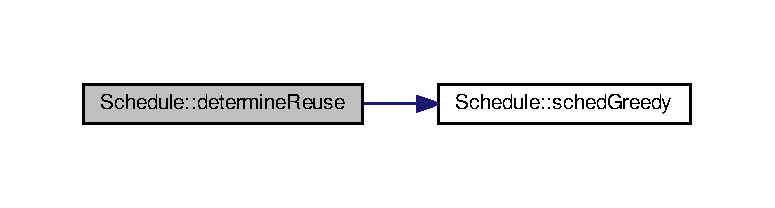
\includegraphics[width=350pt]{classSchedule_a2f1dfef54409f093d3900169af84b850_cgraph}
\end{center}
\end{figure}


\hypertarget{classSchedule_ac301aeb664a5c22bdd0d91aa794d5f7d}{\index{Schedule@{Schedule}!sched\-Greedy@{sched\-Greedy}}
\index{sched\-Greedy@{sched\-Greedy}!Schedule@{Schedule}}
\subsubsection[{sched\-Greedy}]{\setlength{\rightskip}{0pt plus 5cm}bool Schedule\-::sched\-Greedy (
\begin{DoxyParamCaption}
\item[{int $\ast$}]{out\-I\-D, }
\item[{int $\ast$}]{out\-Instance\-Cluster}
\end{DoxyParamCaption}
)\hspace{0.3cm}{\ttfamily [private]}}}\label{classSchedule_ac301aeb664a5c22bdd0d91aa794d5f7d}
The schedule type\-: only use greedy schedule from the paper 

\subsection{Field Documentation}
\hypertarget{classSchedule_a2077242582962c5100fd8d5b086398cb}{\index{Schedule@{Schedule}!cluster\-Scratch\-List@{cluster\-Scratch\-List}}
\index{cluster\-Scratch\-List@{cluster\-Scratch\-List}!Schedule@{Schedule}}
\subsubsection[{cluster\-Scratch\-List}]{\setlength{\rightskip}{0pt plus 5cm}std\-::vector$<$bool$>$ Schedule\-::cluster\-Scratch\-List\hspace{0.3cm}{\ttfamily [private]}}}\label{classSchedule_a2077242582962c5100fd8d5b086398cb}
Corresponding list of variants that must be clustered from scratch \hypertarget{classSchedule_a6be64e3a9e572d346e11481b49d55b7f}{\index{Schedule@{Schedule}!exp\-Ptr@{exp\-Ptr}}
\index{exp\-Ptr@{exp\-Ptr}!Schedule@{Schedule}}
\subsubsection[{exp\-Ptr}]{\setlength{\rightskip}{0pt plus 5cm}std\-::vector$<$struct {\bf experiment}$>$$\ast$ Schedule\-::exp\-Ptr}}\label{classSchedule_a6be64e3a9e572d346e11481b49d55b7f}
Pointer to the vector of defined variants \hypertarget{classSchedule_a0e3d2c52318e5c7060c9fa9ea4e9956b}{\index{Schedule@{Schedule}!finished\-List@{finished\-List}}
\index{finished\-List@{finished\-List}!Schedule@{Schedule}}
\subsubsection[{finished\-List}]{\setlength{\rightskip}{0pt plus 5cm}std\-::vector$<$bool$>$ Schedule\-::finished\-List}}\label{classSchedule_a0e3d2c52318e5c7060c9fa9ea4e9956b}
Keeps track of variants that have completely finished \hypertarget{classSchedule_a5ee0c3a418d3d356c972f09ba4bd1513}{\index{Schedule@{Schedule}!job\-Queue@{job\-Queue}}
\index{job\-Queue@{job\-Queue}!Schedule@{Schedule}}
\subsubsection[{job\-Queue}]{\setlength{\rightskip}{0pt plus 5cm}std\-::queue$<$int$>$ Schedule\-::job\-Queue\hspace{0.3cm}{\ttfamily [private]}}}\label{classSchedule_a5ee0c3a418d3d356c972f09ba4bd1513}
Queue for variant priority ordering \hypertarget{classSchedule_a3bb97864bd4c176f2c55180671abd0a5}{\index{Schedule@{Schedule}!priority\-List@{priority\-List}}
\index{priority\-List@{priority\-List}!Schedule@{Schedule}}
\subsubsection[{priority\-List}]{\setlength{\rightskip}{0pt plus 5cm}std\-::vector$<$int$>$ Schedule\-::priority\-List\hspace{0.3cm}{\ttfamily [private]}}}\label{classSchedule_a3bb97864bd4c176f2c55180671abd0a5}
The order in which the variants should be clustered; stores the ids of the variant list 

The documentation for this class was generated from the following files\-:\begin{DoxyCompactItemize}
\item 
\hyperlink{schedule_8h}{schedule.\-h}\item 
\hyperlink{schedule_8cpp}{schedule.\-cpp}\end{DoxyCompactItemize}

\hypertarget{structRTree_1_1Iterator_1_1StackElement}{\section{R\-Tree$<$ D\-A\-T\-A\-T\-Y\-P\-E, E\-L\-E\-M\-T\-Y\-P\-E, N\-U\-M\-D\-I\-M\-S, E\-L\-E\-M\-T\-Y\-P\-E\-R\-E\-A\-L, T\-M\-A\-X\-N\-O\-D\-E\-S, T\-M\-I\-N\-N\-O\-D\-E\-S $>$\-:\-:Iterator\-:\-:Stack\-Element Struct Reference}
\label{structRTree_1_1Iterator_1_1StackElement}\index{R\-Tree$<$ D\-A\-T\-A\-T\-Y\-P\-E, E\-L\-E\-M\-T\-Y\-P\-E, N\-U\-M\-D\-I\-M\-S, E\-L\-E\-M\-T\-Y\-P\-E\-R\-E\-A\-L, T\-M\-A\-X\-N\-O\-D\-E\-S, T\-M\-I\-N\-N\-O\-D\-E\-S $>$\-::\-Iterator\-::\-Stack\-Element@{R\-Tree$<$ D\-A\-T\-A\-T\-Y\-P\-E, E\-L\-E\-M\-T\-Y\-P\-E, N\-U\-M\-D\-I\-M\-S, E\-L\-E\-M\-T\-Y\-P\-E\-R\-E\-A\-L, T\-M\-A\-X\-N\-O\-D\-E\-S, T\-M\-I\-N\-N\-O\-D\-E\-S $>$\-::\-Iterator\-::\-Stack\-Element}}
}


Collaboration diagram for R\-Tree$<$ D\-A\-T\-A\-T\-Y\-P\-E, E\-L\-E\-M\-T\-Y\-P\-E, N\-U\-M\-D\-I\-M\-S, E\-L\-E\-M\-T\-Y\-P\-E\-R\-E\-A\-L, T\-M\-A\-X\-N\-O\-D\-E\-S, T\-M\-I\-N\-N\-O\-D\-E\-S $>$\-:\-:Iterator\-:\-:Stack\-Element\-:\nopagebreak
\begin{figure}[H]
\begin{center}
\leavevmode
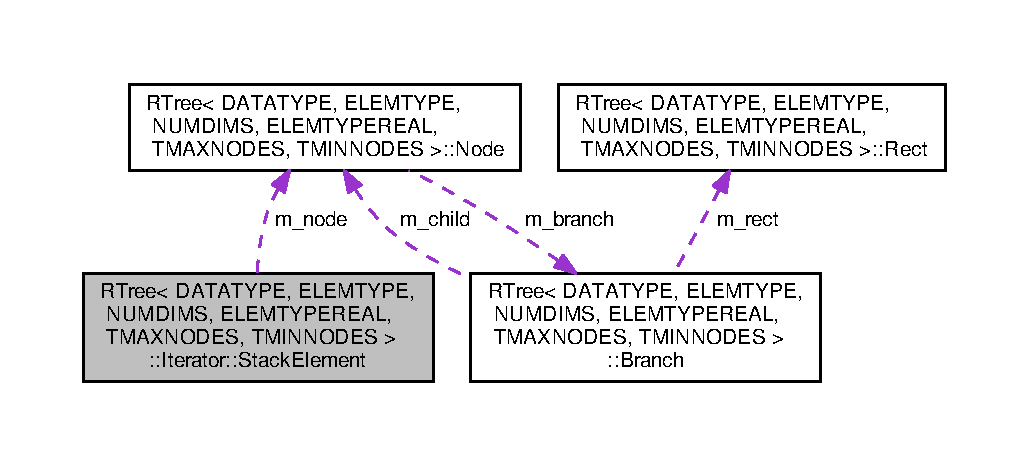
\includegraphics[width=350pt]{structRTree_1_1Iterator_1_1StackElement__coll__graph}
\end{center}
\end{figure}
\subsection*{Data Fields}
\begin{DoxyCompactItemize}
\item 
\hyperlink{structRTree_1_1Node}{Node} $\ast$ \hyperlink{structRTree_1_1Iterator_1_1StackElement_a915f96106d5c78e14209c4d5e83ee756}{m\-\_\-node}
\item 
int \hyperlink{structRTree_1_1Iterator_1_1StackElement_a2101e49f2ac3911fa909a1779485d8f4}{m\-\_\-branch\-Index}
\end{DoxyCompactItemize}


\subsection{Field Documentation}
\hypertarget{structRTree_1_1Iterator_1_1StackElement_a2101e49f2ac3911fa909a1779485d8f4}{\index{R\-Tree\-::\-Iterator\-::\-Stack\-Element@{R\-Tree\-::\-Iterator\-::\-Stack\-Element}!m\-\_\-branch\-Index@{m\-\_\-branch\-Index}}
\index{m\-\_\-branch\-Index@{m\-\_\-branch\-Index}!RTree::Iterator::StackElement@{R\-Tree\-::\-Iterator\-::\-Stack\-Element}}
\subsubsection[{m\-\_\-branch\-Index}]{\setlength{\rightskip}{0pt plus 5cm}template$<$class D\-A\-T\-A\-T\-Y\-P\-E, class E\-L\-E\-M\-T\-Y\-P\-E, int N\-U\-M\-D\-I\-M\-S, class E\-L\-E\-M\-T\-Y\-P\-E\-R\-E\-A\-L = E\-L\-E\-M\-T\-Y\-P\-E, int T\-M\-A\-X\-N\-O\-D\-E\-S = 8, int T\-M\-I\-N\-N\-O\-D\-E\-S = T\-M\-A\-X\-N\-O\-D\-E\-S / 2$>$ int {\bf R\-Tree}$<$ D\-A\-T\-A\-T\-Y\-P\-E, E\-L\-E\-M\-T\-Y\-P\-E, N\-U\-M\-D\-I\-M\-S, E\-L\-E\-M\-T\-Y\-P\-E\-R\-E\-A\-L, T\-M\-A\-X\-N\-O\-D\-E\-S, T\-M\-I\-N\-N\-O\-D\-E\-S $>$\-::Iterator\-::\-Stack\-Element\-::m\-\_\-branch\-Index}}\label{structRTree_1_1Iterator_1_1StackElement_a2101e49f2ac3911fa909a1779485d8f4}
\hypertarget{structRTree_1_1Iterator_1_1StackElement_a915f96106d5c78e14209c4d5e83ee756}{\index{R\-Tree\-::\-Iterator\-::\-Stack\-Element@{R\-Tree\-::\-Iterator\-::\-Stack\-Element}!m\-\_\-node@{m\-\_\-node}}
\index{m\-\_\-node@{m\-\_\-node}!RTree::Iterator::StackElement@{R\-Tree\-::\-Iterator\-::\-Stack\-Element}}
\subsubsection[{m\-\_\-node}]{\setlength{\rightskip}{0pt plus 5cm}template$<$class D\-A\-T\-A\-T\-Y\-P\-E, class E\-L\-E\-M\-T\-Y\-P\-E, int N\-U\-M\-D\-I\-M\-S, class E\-L\-E\-M\-T\-Y\-P\-E\-R\-E\-A\-L = E\-L\-E\-M\-T\-Y\-P\-E, int T\-M\-A\-X\-N\-O\-D\-E\-S = 8, int T\-M\-I\-N\-N\-O\-D\-E\-S = T\-M\-A\-X\-N\-O\-D\-E\-S / 2$>$ {\bf Node}$\ast$ {\bf R\-Tree}$<$ D\-A\-T\-A\-T\-Y\-P\-E, E\-L\-E\-M\-T\-Y\-P\-E, N\-U\-M\-D\-I\-M\-S, E\-L\-E\-M\-T\-Y\-P\-E\-R\-E\-A\-L, T\-M\-A\-X\-N\-O\-D\-E\-S, T\-M\-I\-N\-N\-O\-D\-E\-S $>$\-::Iterator\-::\-Stack\-Element\-::m\-\_\-node}}\label{structRTree_1_1Iterator_1_1StackElement_a915f96106d5c78e14209c4d5e83ee756}


The documentation for this struct was generated from the following file\-:\begin{DoxyCompactItemize}
\item 
\hyperlink{RTree_8h}{R\-Tree.\-h}\end{DoxyCompactItemize}

\chapter{File Documentation}
\hypertarget{c__test__prog_8cpp}{\section{c\-\_\-test\-\_\-prog.\-cpp File Reference}
\label{c__test__prog_8cpp}\index{c\-\_\-test\-\_\-prog.\-cpp@{c\-\_\-test\-\_\-prog.\-cpp}}
}
{\ttfamily \#include $<$vector$>$}\\*
{\ttfamily \#include $<$stdio.\-h$>$}\\*
{\ttfamily \#include $<$string.\-h$>$}\\*
{\ttfamily \#include $<$cstdlib$>$}\\*
{\ttfamily \#include $<$dlfcn.\-h$>$}\\*
{\ttfamily \#include \char`\"{}structs.\-h\char`\"{}}\\*
{\ttfamily \#include \char`\"{}c\-\_\-test\-\_\-prog.\-h\char`\"{}}\\*
Include dependency graph for c\-\_\-test\-\_\-prog.\-cpp\-:\nopagebreak
\begin{figure}[H]
\begin{center}
\leavevmode
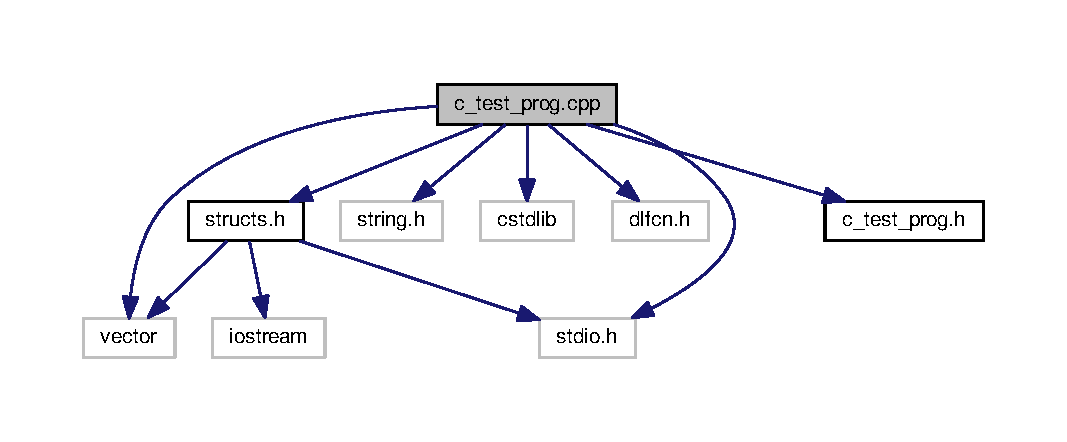
\includegraphics[width=350pt]{c__test__prog_8cpp__incl}
\end{center}
\end{figure}
\subsection*{Functions}
\begin{DoxyCompactItemize}
\item 
int \hyperlink{c__test__prog_8cpp_ae66f6b31b5ad750f1fe042a706a4e3d4}{main} ()
\end{DoxyCompactItemize}


\subsection{Function Documentation}
\hypertarget{c__test__prog_8cpp_ae66f6b31b5ad750f1fe042a706a4e3d4}{\index{c\-\_\-test\-\_\-prog.\-cpp@{c\-\_\-test\-\_\-prog.\-cpp}!main@{main}}
\index{main@{main}!c_test_prog.cpp@{c\-\_\-test\-\_\-prog.\-cpp}}
\subsubsection[{main}]{\setlength{\rightskip}{0pt plus 5cm}int main (
\begin{DoxyParamCaption}
{}
\end{DoxyParamCaption}
)}}\label{c__test__prog_8cpp_ae66f6b31b5ad750f1fe042a706a4e3d4}


Here is the call graph for this function\-:\nopagebreak
\begin{figure}[H]
\begin{center}
\leavevmode
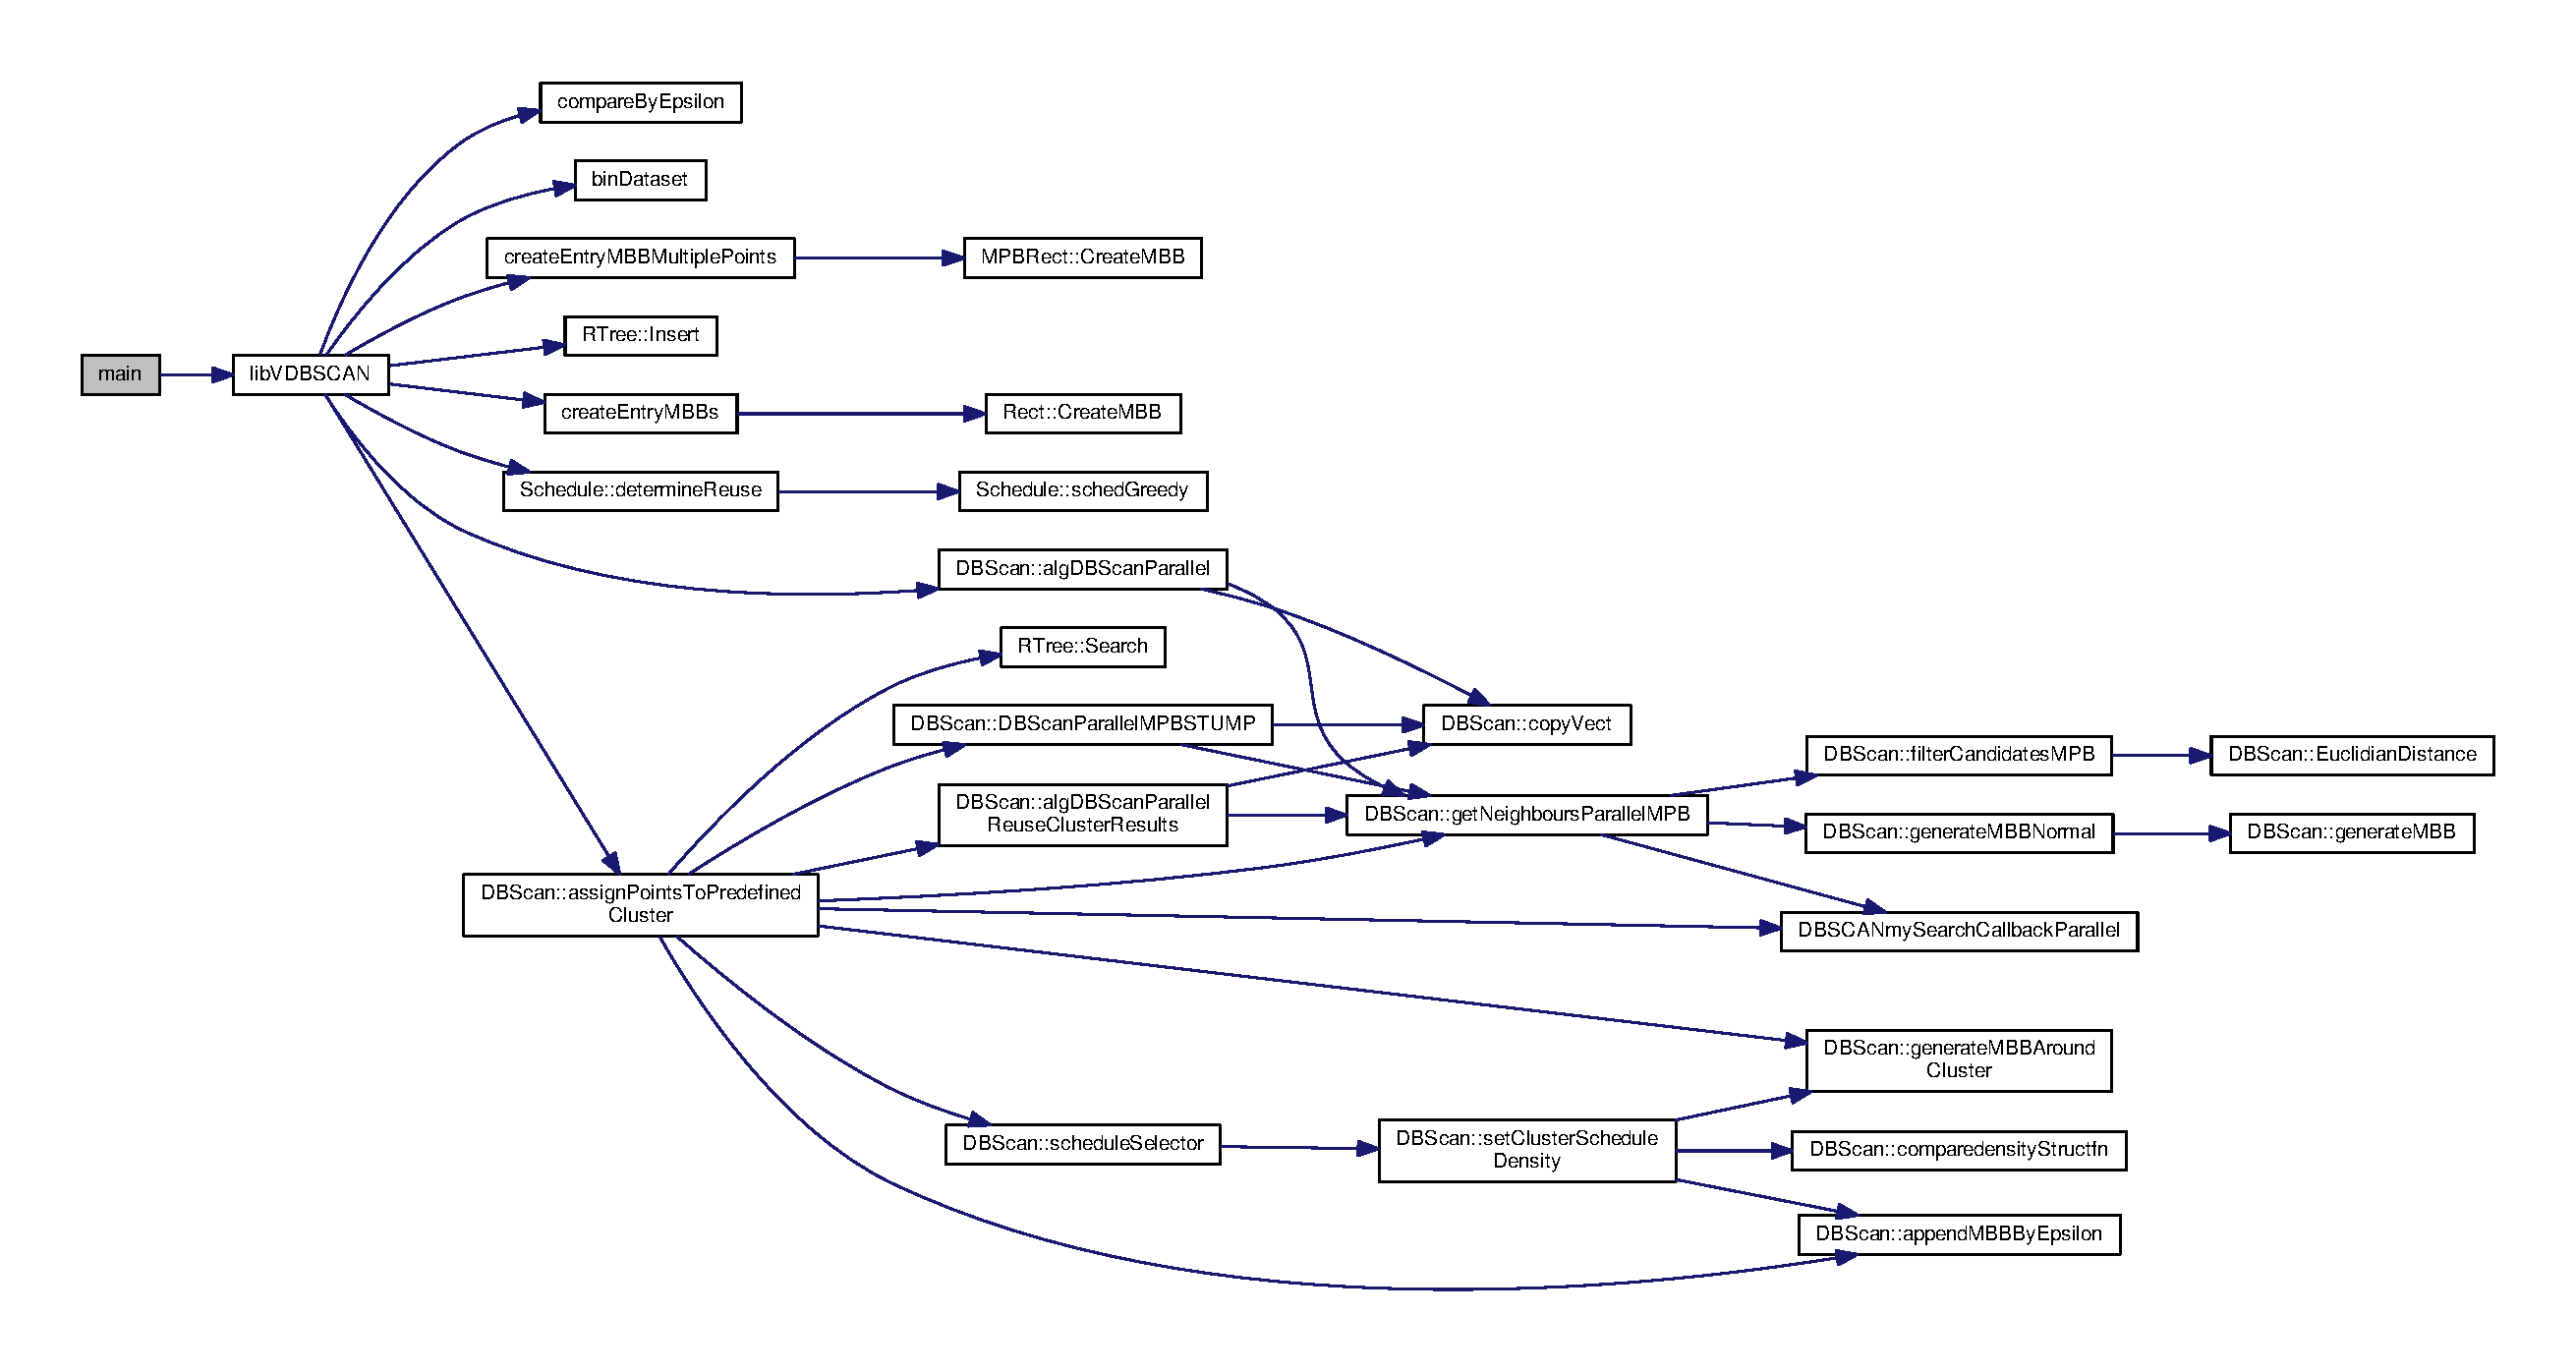
\includegraphics[width=350pt]{c__test__prog_8cpp_ae66f6b31b5ad750f1fe042a706a4e3d4_cgraph}
\end{center}
\end{figure}



\hypertarget{c__test__prog_8h}{\section{c\-\_\-test\-\_\-prog.\-h File Reference}
\label{c__test__prog_8h}\index{c\-\_\-test\-\_\-prog.\-h@{c\-\_\-test\-\_\-prog.\-h}}
}
This graph shows which files directly or indirectly include this file\-:\nopagebreak
\begin{figure}[H]
\begin{center}
\leavevmode
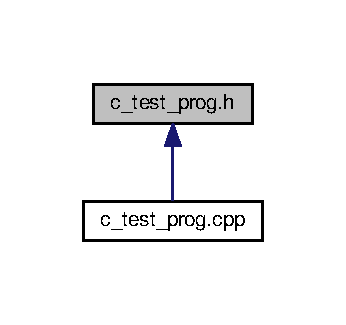
\includegraphics[width=166pt]{c__test__prog_8h__dep__incl}
\end{center}
\end{figure}
\subsection*{Functions}
\begin{DoxyCompactItemize}
\item 
int \hyperlink{c__test__prog_8h_a2a1fa7bbb574f193ee87a385a0c0f06b}{lib\-V\-D\-B\-S\-C\-A\-N} (double $\ast$inputx, double $\ast$inputy, unsigned int dataset\-Size, double $\ast$input\-Epsilon, unsigned int $\ast$input\-Minpts, unsigned int num\-Variants, int M\-B\-Bsize, unsigned int $\ast$ret\-Arr, bool verbose)
\end{DoxyCompactItemize}


\subsection{Function Documentation}
\hypertarget{c__test__prog_8h_a2a1fa7bbb574f193ee87a385a0c0f06b}{\index{c\-\_\-test\-\_\-prog.\-h@{c\-\_\-test\-\_\-prog.\-h}!lib\-V\-D\-B\-S\-C\-A\-N@{lib\-V\-D\-B\-S\-C\-A\-N}}
\index{lib\-V\-D\-B\-S\-C\-A\-N@{lib\-V\-D\-B\-S\-C\-A\-N}!c_test_prog.h@{c\-\_\-test\-\_\-prog.\-h}}
\subsubsection[{lib\-V\-D\-B\-S\-C\-A\-N}]{\setlength{\rightskip}{0pt plus 5cm}int lib\-V\-D\-B\-S\-C\-A\-N (
\begin{DoxyParamCaption}
\item[{double $\ast$}]{inputx, }
\item[{double $\ast$}]{inputy, }
\item[{unsigned int}]{dataset\-Size, }
\item[{double $\ast$}]{input\-Epsilon, }
\item[{unsigned int $\ast$}]{input\-Minpts, }
\item[{unsigned int}]{num\-Variants, }
\item[{int}]{M\-B\-Bsize, }
\item[{unsigned int $\ast$}]{ret\-Arr, }
\item[{bool}]{verbose}
\end{DoxyParamCaption}
)}}\label{c__test__prog_8h_a2a1fa7bbb574f193ee87a385a0c0f06b}


Here is the call graph for this function\-:\nopagebreak
\begin{figure}[H]
\begin{center}
\leavevmode
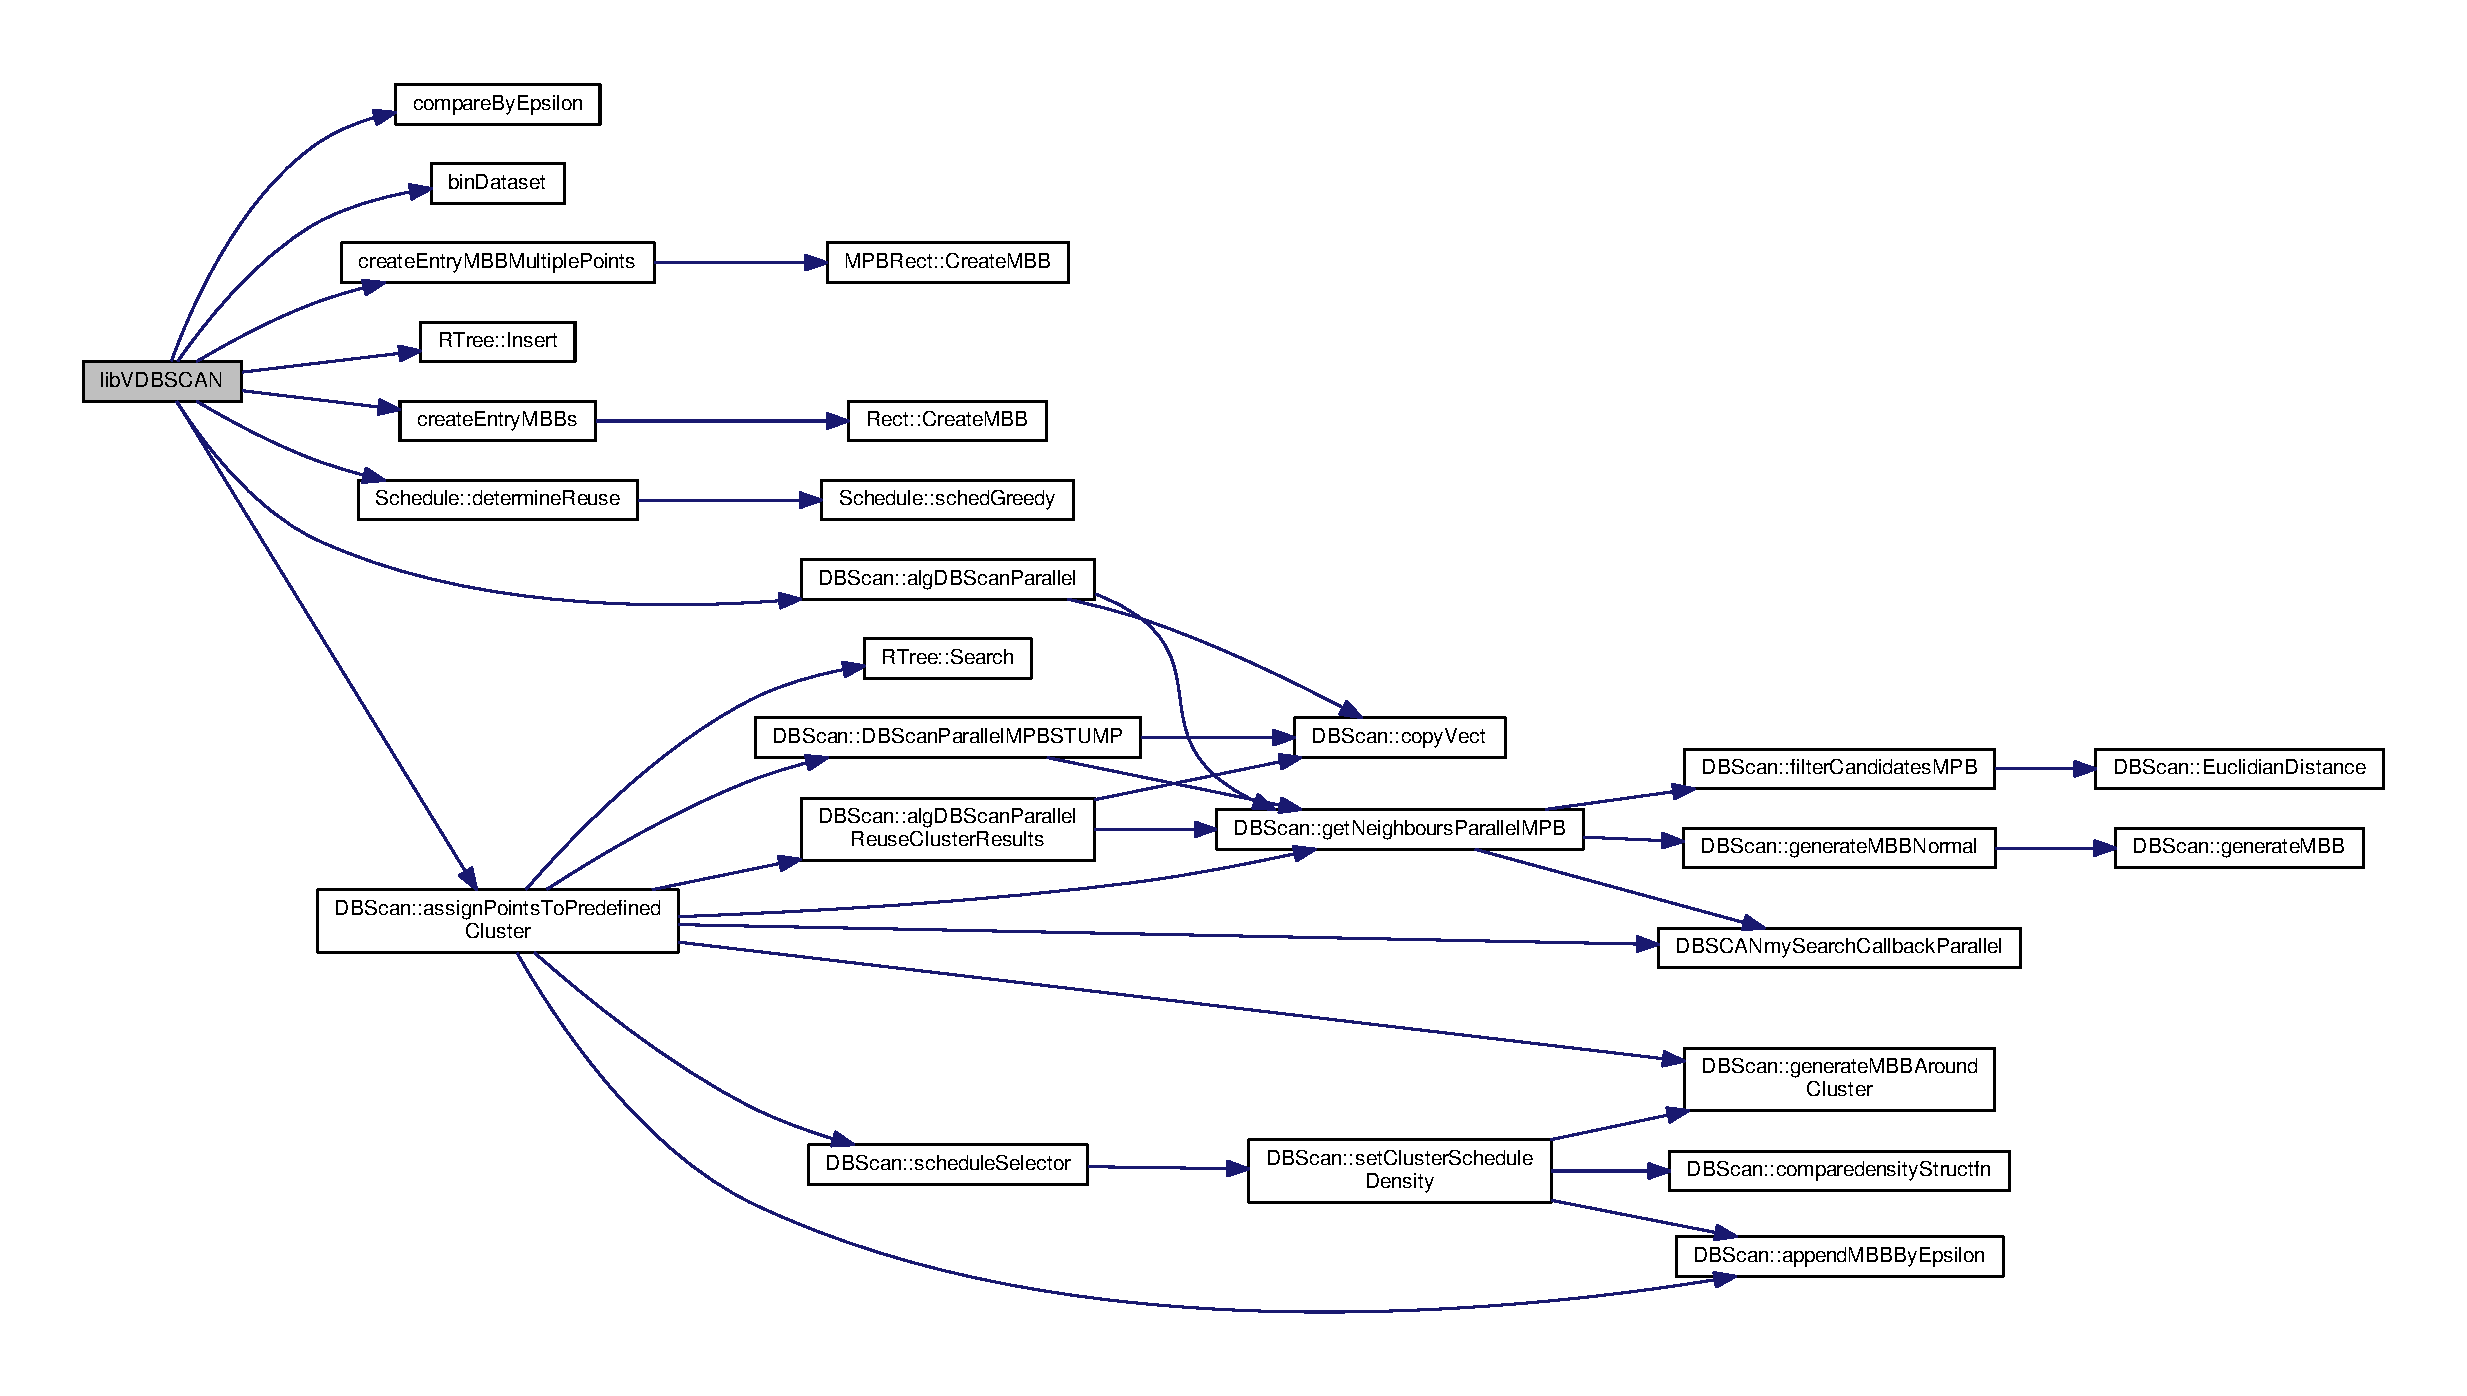
\includegraphics[width=350pt]{c__test__prog_8h_a2a1fa7bbb574f193ee87a385a0c0f06b_cgraph}
\end{center}
\end{figure}



\hypertarget{DBScan_8cpp}{\section{D\-B\-Scan.\-cpp File Reference}
\label{DBScan_8cpp}\index{D\-B\-Scan.\-cpp@{D\-B\-Scan.\-cpp}}
}
{\ttfamily \#include \char`\"{}structs.\-h\char`\"{}}\\*
{\ttfamily \#include \char`\"{}prototypes.\-h\char`\"{}}\\*
{\ttfamily \#include \char`\"{}globals.\-h\char`\"{}}\\*
{\ttfamily \#include $<$fstream$>$}\\*
{\ttfamily \#include $<$vector$>$}\\*
{\ttfamily \#include $<$set$>$}\\*
{\ttfamily \#include \char`\"{}R\-Tree.\-h\char`\"{}}\\*
{\ttfamily \#include \char`\"{}D\-B\-Scan.\-h\char`\"{}}\\*
{\ttfamily \#include $<$omp.\-h$>$}\\*
{\ttfamily \#include $<$iostream$>$}\\*
{\ttfamily \#include $<$unistd.\-h$>$}\\*
Include dependency graph for D\-B\-Scan.\-cpp\-:\nopagebreak
\begin{figure}[H]
\begin{center}
\leavevmode
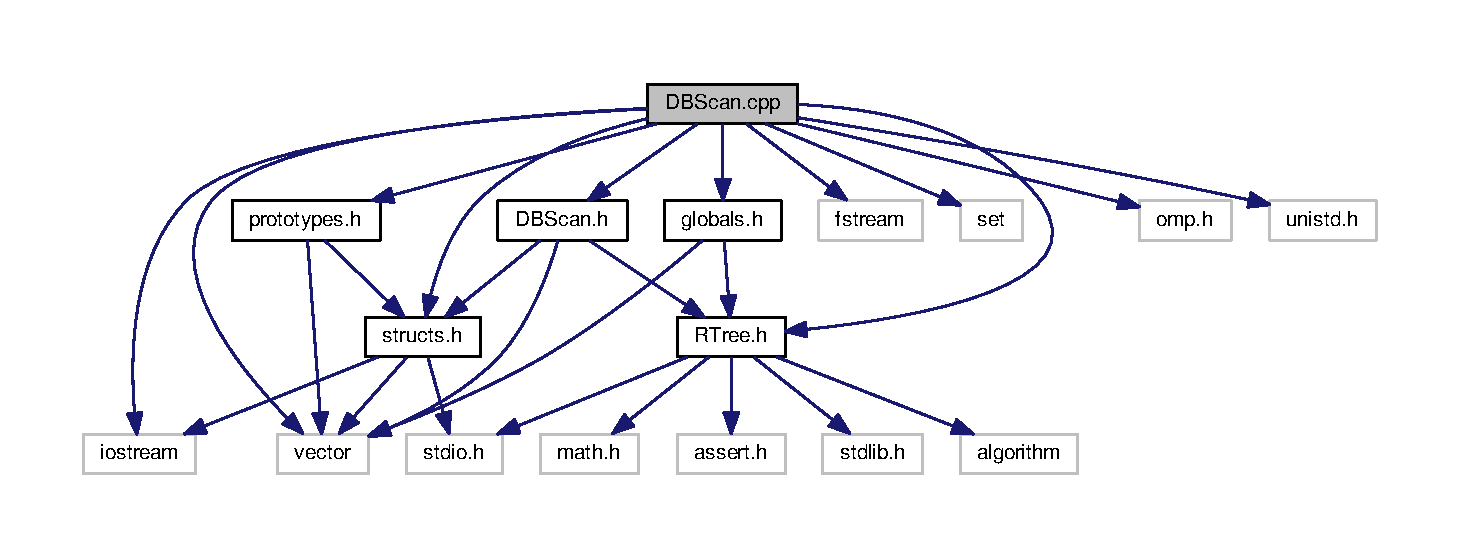
\includegraphics[width=350pt]{DBScan_8cpp__incl}
\end{center}
\end{figure}
\subsection*{Variables}
\begin{DoxyCompactItemize}
\item 
const int \hyperlink{DBScan_8cpp_af9cfd37b7d8ec7350c9c03f7396dfd4f}{N\-U\-M\-M\-I\-N\-R\-E\-U\-S\-E\-P\-T\-S} =100
\item 
std\-::vector$<$ int $>$ \hyperlink{DBScan_8cpp_aea636a4db974aa94b19bd2f1f06e0ff1}{neighbour\-List}
\item 
std\-::vector$<$ int $>$ \hyperlink{DBScan_8cpp_a1e7b0a62b9706f13c1f2dc5cdf37336b}{neighbour\-List\-Parallel} \mbox{[}N\-S\-E\-A\-R\-C\-H\-T\-H\-R\-E\-A\-D\-S\mbox{]}
\end{DoxyCompactItemize}


\subsection{Variable Documentation}
\hypertarget{DBScan_8cpp_aea636a4db974aa94b19bd2f1f06e0ff1}{\index{D\-B\-Scan.\-cpp@{D\-B\-Scan.\-cpp}!neighbour\-List@{neighbour\-List}}
\index{neighbour\-List@{neighbour\-List}!DBScan.cpp@{D\-B\-Scan.\-cpp}}
\subsubsection[{neighbour\-List}]{\setlength{\rightskip}{0pt plus 5cm}std\-::vector$<$int$>$ neighbour\-List}}\label{DBScan_8cpp_aea636a4db974aa94b19bd2f1f06e0ff1}
\hypertarget{DBScan_8cpp_a1e7b0a62b9706f13c1f2dc5cdf37336b}{\index{D\-B\-Scan.\-cpp@{D\-B\-Scan.\-cpp}!neighbour\-List\-Parallel@{neighbour\-List\-Parallel}}
\index{neighbour\-List\-Parallel@{neighbour\-List\-Parallel}!DBScan.cpp@{D\-B\-Scan.\-cpp}}
\subsubsection[{neighbour\-List\-Parallel}]{\setlength{\rightskip}{0pt plus 5cm}std\-::vector$<$int$>$ neighbour\-List\-Parallel\mbox{[}N\-S\-E\-A\-R\-C\-H\-T\-H\-R\-E\-A\-D\-S\mbox{]}}}\label{DBScan_8cpp_a1e7b0a62b9706f13c1f2dc5cdf37336b}
\hypertarget{DBScan_8cpp_af9cfd37b7d8ec7350c9c03f7396dfd4f}{\index{D\-B\-Scan.\-cpp@{D\-B\-Scan.\-cpp}!N\-U\-M\-M\-I\-N\-R\-E\-U\-S\-E\-P\-T\-S@{N\-U\-M\-M\-I\-N\-R\-E\-U\-S\-E\-P\-T\-S}}
\index{N\-U\-M\-M\-I\-N\-R\-E\-U\-S\-E\-P\-T\-S@{N\-U\-M\-M\-I\-N\-R\-E\-U\-S\-E\-P\-T\-S}!DBScan.cpp@{D\-B\-Scan.\-cpp}}
\subsubsection[{N\-U\-M\-M\-I\-N\-R\-E\-U\-S\-E\-P\-T\-S}]{\setlength{\rightskip}{0pt plus 5cm}const int N\-U\-M\-M\-I\-N\-R\-E\-U\-S\-E\-P\-T\-S =100}}\label{DBScan_8cpp_af9cfd37b7d8ec7350c9c03f7396dfd4f}

\hypertarget{DBScan_8h}{\section{D\-B\-Scan.\-h File Reference}
\label{DBScan_8h}\index{D\-B\-Scan.\-h@{D\-B\-Scan.\-h}}
}
{\ttfamily \#include \char`\"{}structs.\-h\char`\"{}}\\*
{\ttfamily \#include $<$vector$>$}\\*
{\ttfamily \#include \char`\"{}R\-Tree.\-h\char`\"{}}\\*
Include dependency graph for D\-B\-Scan.\-h\-:\nopagebreak
\begin{figure}[H]
\begin{center}
\leavevmode
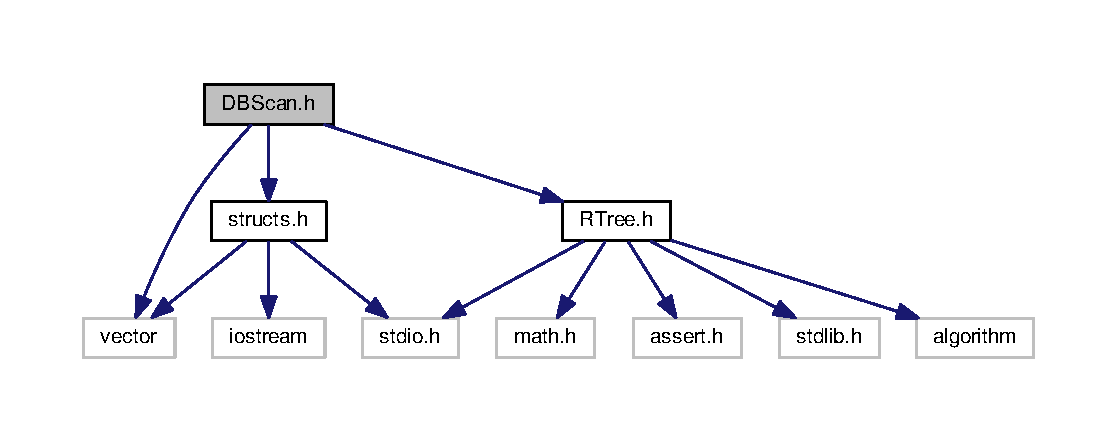
\includegraphics[width=350pt]{DBScan_8h__incl}
\end{center}
\end{figure}
This graph shows which files directly or indirectly include this file\-:\nopagebreak
\begin{figure}[H]
\begin{center}
\leavevmode
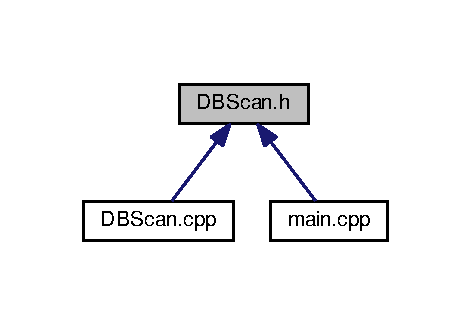
\includegraphics[width=226pt]{DBScan_8h__dep__incl}
\end{center}
\end{figure}
\subsection*{Data Structures}
\begin{DoxyCompactItemize}
\item 
class \hyperlink{classDBScan}{D\-B\-Scan}
\end{DoxyCompactItemize}

\hypertarget{globals_8h}{\section{globals.\-h File Reference}
\label{globals_8h}\index{globals.\-h@{globals.\-h}}
}
{\ttfamily \#include $<$vector$>$}\\*
{\ttfamily \#include \char`\"{}R\-Tree.\-h\char`\"{}}\\*
Include dependency graph for globals.\-h\-:\nopagebreak
\begin{figure}[H]
\begin{center}
\leavevmode
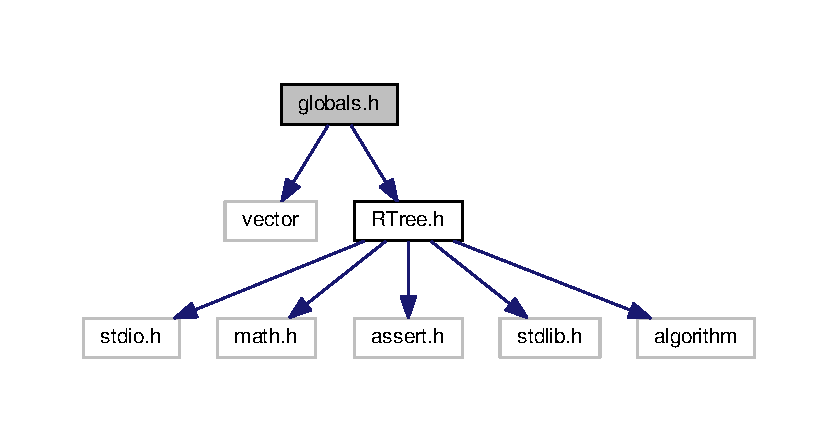
\includegraphics[width=350pt]{globals_8h__incl}
\end{center}
\end{figure}
This graph shows which files directly or indirectly include this file\-:\nopagebreak
\begin{figure}[H]
\begin{center}
\leavevmode
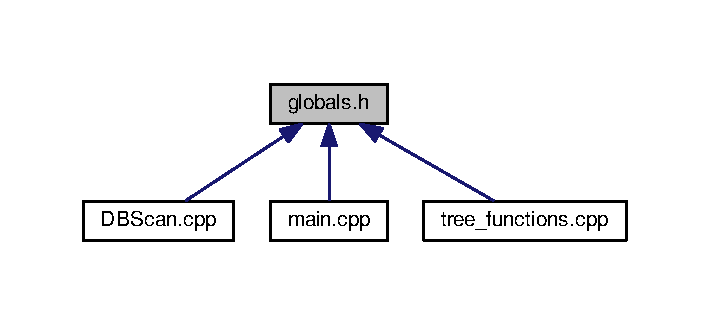
\includegraphics[width=340pt]{globals_8h__dep__incl}
\end{center}
\end{figure}
\subsection*{Variables}
\begin{DoxyCompactItemize}
\item 
struct \hyperlink{structdataElem}{data\-Elem} $\ast$ \hyperlink{globals_8h_ac152ac2be0eb07c2b73b4bb54a8f1952}{data\-Points}
\item 
std\-::vector$<$ int $>$ \hyperlink{globals_8h_a9af604b800745c5af23200044809a540}{neighbour\-List\-Parallel} \mbox{[}$\,$\mbox{]}
\end{DoxyCompactItemize}


\subsection{Variable Documentation}
\hypertarget{globals_8h_ac152ac2be0eb07c2b73b4bb54a8f1952}{\index{globals.\-h@{globals.\-h}!data\-Points@{data\-Points}}
\index{data\-Points@{data\-Points}!globals.h@{globals.\-h}}
\subsubsection[{data\-Points}]{\setlength{\rightskip}{0pt plus 5cm}struct {\bf data\-Elem}$\ast$ data\-Points}}\label{globals_8h_ac152ac2be0eb07c2b73b4bb54a8f1952}
\hypertarget{globals_8h_a9af604b800745c5af23200044809a540}{\index{globals.\-h@{globals.\-h}!neighbour\-List\-Parallel@{neighbour\-List\-Parallel}}
\index{neighbour\-List\-Parallel@{neighbour\-List\-Parallel}!globals.h@{globals.\-h}}
\subsubsection[{neighbour\-List\-Parallel}]{\setlength{\rightskip}{0pt plus 5cm}std\-::vector$<$int$>$ neighbour\-List\-Parallel\mbox{[}$\,$\mbox{]}}}\label{globals_8h_a9af604b800745c5af23200044809a540}

\hypertarget{main_8cpp}{\section{main.\-cpp File Reference}
\label{main_8cpp}\index{main.\-cpp@{main.\-cpp}}
}
{\ttfamily \#include $<$math.\-h$>$}\\*
{\ttfamily \#include $<$cstdlib$>$}\\*
{\ttfamily \#include $<$stdio.\-h$>$}\\*
{\ttfamily \#include \char`\"{}prototypes.\-h\char`\"{}}\\*
{\ttfamily \#include \char`\"{}globals.\-h\char`\"{}}\\*
{\ttfamily \#include \char`\"{}R\-Tree.\-h\char`\"{}}\\*
{\ttfamily \#include \char`\"{}omp.\-h\char`\"{}}\\*
{\ttfamily \#include \char`\"{}D\-B\-Scan.\-h\char`\"{}}\\*
{\ttfamily \#include \char`\"{}schedule.\-h\char`\"{}}\\*
{\ttfamily \#include $<$algorithm$>$}\\*
{\ttfamily \#include $<$string.\-h$>$}\\*
{\ttfamily \#include $<$fstream$>$}\\*
{\ttfamily \#include $<$iostream$>$}\\*
{\ttfamily \#include $<$string$>$}\\*
{\ttfamily \#include $<$limits$>$}\\*
Include dependency graph for main.\-cpp\-:\nopagebreak
\begin{figure}[H]
\begin{center}
\leavevmode
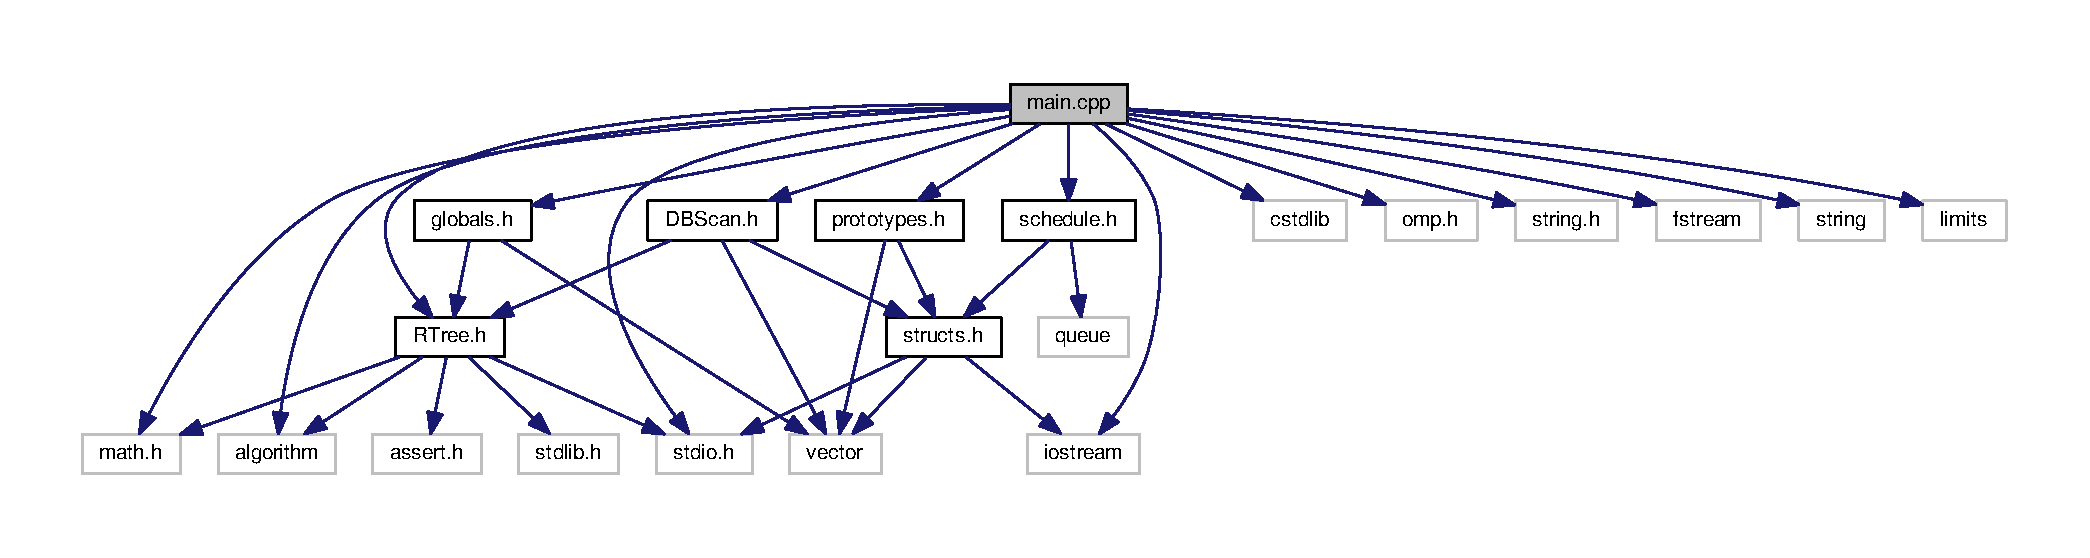
\includegraphics[width=350pt]{main_8cpp__incl}
\end{center}
\end{figure}
\subsection*{Functions}
\begin{DoxyCompactItemize}
\item 
int \hyperlink{main_8cpp_a2a1fa7bbb574f193ee87a385a0c0f06b}{lib\-V\-D\-B\-S\-C\-A\-N} (double $\ast$inputx, double $\ast$inputy, unsigned int dataset\-Size, double $\ast$input\-Epsilon, unsigned int $\ast$input\-Minpts, unsigned int num\-Variants, int M\-B\-Bsize, unsigned int $\ast$ret\-Arr, bool verbose)
\item 
void \hyperlink{main_8cpp_afa8668a508acc63abb9a705f8f643656}{create\-Entry\-M\-B\-B\-Multiple\-Points} (std\-::vector$<$ \hyperlink{structdataElem}{data\-Elem} $>$ $\ast$\hyperlink{globals_8h_ac152ac2be0eb07c2b73b4bb54a8f1952}{data\-Points}, std\-::vector$<$ std\-::vector$<$ int $>$ $>$ $\ast$M\-P\-B\-\_\-ids, \hyperlink{structMPBRect}{M\-P\-B\-Rect} $\ast$data\-Rects\-M\-P\-B, int M\-B\-B\-Size)
\begin{DoxyCompactList}\small\item\em Generates M\-B\-Bs for for the R-\/tree when indexing multiple points per M\-B\-B. \end{DoxyCompactList}\item 
void \hyperlink{main_8cpp_a8c639584f626e061f0aead36ffa60038}{create\-Entry\-M\-B\-Bs} (std\-::vector$<$ \hyperlink{structdataElem}{data\-Elem} $>$ $\ast$\hyperlink{globals_8h_ac152ac2be0eb07c2b73b4bb54a8f1952}{data\-Points}, \hyperlink{structRect}{Rect} $\ast$data\-Rects)
\begin{DoxyCompactList}\small\item\em Generates M\-B\-Bs for the R-\/tree. \end{DoxyCompactList}\item 
void \hyperlink{main_8cpp_a6ad8dcc1d9af410f2f4640967a4620a6}{bin\-Dataset} (std\-::vector$<$ \hyperlink{structdataElem}{data\-Elem} $>$ $\ast$\hyperlink{globals_8h_ac152ac2be0eb07c2b73b4bb54a8f1952}{data\-Points}, int num\-Bins, std\-::vector$<$ int $>$ $\ast$mapping, bool verbose)
\begin{DoxyCompactList}\small\item\em Bins the 2-\/\-D input dataset, and keeps track of where the points in space were mapped to the original input dataset. \end{DoxyCompactList}\item 
bool \hyperlink{main_8cpp_a786d2eaac37700e364631015ca72e846}{compare\-By\-Epsilon} (const \hyperlink{structexperiment}{experiment} \&a, const \hyperlink{structexperiment}{experiment} \&b)
\begin{DoxyCompactList}\small\item\em Comparison function for sorting. \end{DoxyCompactList}\item 
bool \hyperlink{main_8cpp_acd7e170375eea7e22e77c1b85f2636bf}{compare\-Data\-Elem\-Struct\-Func} (const \hyperlink{structdataElem}{data\-Elem} \&elem1, const \hyperlink{structdataElem}{data\-Elem} \&elem2)
\begin{DoxyCompactList}\small\item\em Comparison function for sorting. \end{DoxyCompactList}\item 
int \hyperlink{main_8cpp_ab6302c1085a6ee3030e2a1fa2125e07b}{bin\-\_\-x} (double x)
\begin{DoxyCompactList}\small\item\em Used for binning the input dataset. \end{DoxyCompactList}\item 
int \hyperlink{main_8cpp_a1b8bf045673fe0bbea47084f6ae126eb}{bin\-\_\-y} (double x)
\begin{DoxyCompactList}\small\item\em Used for binning the input dataset. \end{DoxyCompactList}\end{DoxyCompactItemize}


\subsection{Function Documentation}
\hypertarget{main_8cpp_ab6302c1085a6ee3030e2a1fa2125e07b}{\index{main.\-cpp@{main.\-cpp}!bin\-\_\-x@{bin\-\_\-x}}
\index{bin\-\_\-x@{bin\-\_\-x}!main.cpp@{main.\-cpp}}
\subsubsection[{bin\-\_\-x}]{\setlength{\rightskip}{0pt plus 5cm}int bin\-\_\-x (
\begin{DoxyParamCaption}
\item[{double}]{x}
\end{DoxyParamCaption}
)}}\label{main_8cpp_ab6302c1085a6ee3030e2a1fa2125e07b}


Used for binning the input dataset. 

\hypertarget{main_8cpp_a1b8bf045673fe0bbea47084f6ae126eb}{\index{main.\-cpp@{main.\-cpp}!bin\-\_\-y@{bin\-\_\-y}}
\index{bin\-\_\-y@{bin\-\_\-y}!main.cpp@{main.\-cpp}}
\subsubsection[{bin\-\_\-y}]{\setlength{\rightskip}{0pt plus 5cm}int bin\-\_\-y (
\begin{DoxyParamCaption}
\item[{double}]{x}
\end{DoxyParamCaption}
)}}\label{main_8cpp_a1b8bf045673fe0bbea47084f6ae126eb}


Used for binning the input dataset. 

\hypertarget{main_8cpp_a6ad8dcc1d9af410f2f4640967a4620a6}{\index{main.\-cpp@{main.\-cpp}!bin\-Dataset@{bin\-Dataset}}
\index{bin\-Dataset@{bin\-Dataset}!main.cpp@{main.\-cpp}}
\subsubsection[{bin\-Dataset}]{\setlength{\rightskip}{0pt plus 5cm}void bin\-Dataset (
\begin{DoxyParamCaption}
\item[{std\-::vector$<$ {\bf data\-Elem} $>$ $\ast$}]{data\-Points, }
\item[{int}]{num\-Bins, }
\item[{std\-::vector$<$ int $>$ $\ast$}]{mapping, }
\item[{bool}]{verbose}
\end{DoxyParamCaption}
)}}\label{main_8cpp_a6ad8dcc1d9af410f2f4640967a4620a6}


Bins the 2-\/\-D input dataset, and keeps track of where the points in space were mapped to the original input dataset. 

\hypertarget{main_8cpp_a786d2eaac37700e364631015ca72e846}{\index{main.\-cpp@{main.\-cpp}!compare\-By\-Epsilon@{compare\-By\-Epsilon}}
\index{compare\-By\-Epsilon@{compare\-By\-Epsilon}!main.cpp@{main.\-cpp}}
\subsubsection[{compare\-By\-Epsilon}]{\setlength{\rightskip}{0pt plus 5cm}bool compare\-By\-Epsilon (
\begin{DoxyParamCaption}
\item[{const {\bf experiment} \&}]{a, }
\item[{const {\bf experiment} \&}]{b}
\end{DoxyParamCaption}
)}}\label{main_8cpp_a786d2eaac37700e364631015ca72e846}


Comparison function for sorting. 

\hypertarget{main_8cpp_acd7e170375eea7e22e77c1b85f2636bf}{\index{main.\-cpp@{main.\-cpp}!compare\-Data\-Elem\-Struct\-Func@{compare\-Data\-Elem\-Struct\-Func}}
\index{compare\-Data\-Elem\-Struct\-Func@{compare\-Data\-Elem\-Struct\-Func}!main.cpp@{main.\-cpp}}
\subsubsection[{compare\-Data\-Elem\-Struct\-Func}]{\setlength{\rightskip}{0pt plus 5cm}bool compare\-Data\-Elem\-Struct\-Func (
\begin{DoxyParamCaption}
\item[{const {\bf data\-Elem} \&}]{elem1, }
\item[{const {\bf data\-Elem} \&}]{elem2}
\end{DoxyParamCaption}
)}}\label{main_8cpp_acd7e170375eea7e22e77c1b85f2636bf}


Comparison function for sorting. 



Here is the call graph for this function\-:
\nopagebreak
\begin{figure}[H]
\begin{center}
\leavevmode
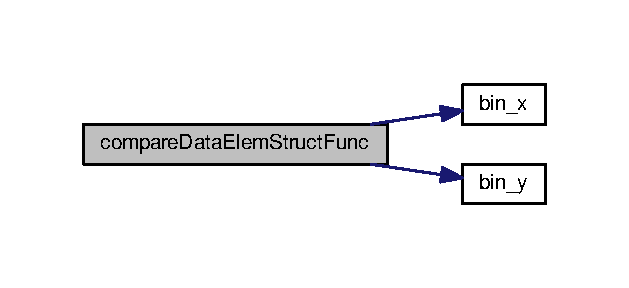
\includegraphics[width=302pt]{main_8cpp_acd7e170375eea7e22e77c1b85f2636bf_cgraph}
\end{center}
\end{figure}


\hypertarget{main_8cpp_afa8668a508acc63abb9a705f8f643656}{\index{main.\-cpp@{main.\-cpp}!create\-Entry\-M\-B\-B\-Multiple\-Points@{create\-Entry\-M\-B\-B\-Multiple\-Points}}
\index{create\-Entry\-M\-B\-B\-Multiple\-Points@{create\-Entry\-M\-B\-B\-Multiple\-Points}!main.cpp@{main.\-cpp}}
\subsubsection[{create\-Entry\-M\-B\-B\-Multiple\-Points}]{\setlength{\rightskip}{0pt plus 5cm}void create\-Entry\-M\-B\-B\-Multiple\-Points (
\begin{DoxyParamCaption}
\item[{std\-::vector$<$ {\bf data\-Elem} $>$ $\ast$}]{data\-Points, }
\item[{std\-::vector$<$ std\-::vector$<$ int $>$ $>$ $\ast$}]{M\-P\-B\-\_\-ids, }
\item[{{\bf M\-P\-B\-Rect} $\ast$}]{data\-Rects\-M\-P\-B, }
\item[{int}]{M\-B\-B\-Size}
\end{DoxyParamCaption}
)}}\label{main_8cpp_afa8668a508acc63abb9a705f8f643656}


Generates M\-B\-Bs for for the R-\/tree when indexing multiple points per M\-B\-B. 



Here is the call graph for this function\-:\nopagebreak
\begin{figure}[H]
\begin{center}
\leavevmode
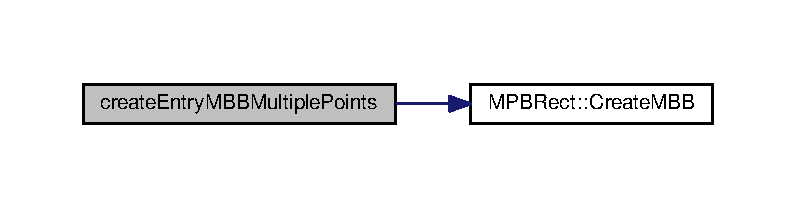
\includegraphics[width=350pt]{main_8cpp_afa8668a508acc63abb9a705f8f643656_cgraph}
\end{center}
\end{figure}


\hypertarget{main_8cpp_a8c639584f626e061f0aead36ffa60038}{\index{main.\-cpp@{main.\-cpp}!create\-Entry\-M\-B\-Bs@{create\-Entry\-M\-B\-Bs}}
\index{create\-Entry\-M\-B\-Bs@{create\-Entry\-M\-B\-Bs}!main.cpp@{main.\-cpp}}
\subsubsection[{create\-Entry\-M\-B\-Bs}]{\setlength{\rightskip}{0pt plus 5cm}void create\-Entry\-M\-B\-Bs (
\begin{DoxyParamCaption}
\item[{std\-::vector$<$ {\bf data\-Elem} $>$ $\ast$}]{data\-Points, }
\item[{{\bf Rect} $\ast$}]{data\-Rects}
\end{DoxyParamCaption}
)}}\label{main_8cpp_a8c639584f626e061f0aead36ffa60038}


Generates M\-B\-Bs for the R-\/tree. 



Here is the call graph for this function\-:\nopagebreak
\begin{figure}[H]
\begin{center}
\leavevmode
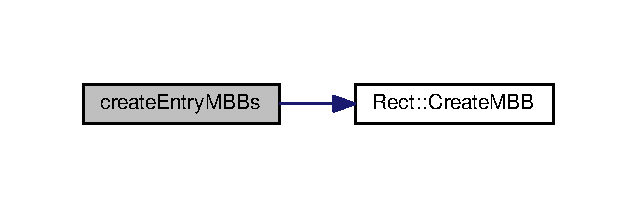
\includegraphics[width=306pt]{main_8cpp_a8c639584f626e061f0aead36ffa60038_cgraph}
\end{center}
\end{figure}


\hypertarget{main_8cpp_a2a1fa7bbb574f193ee87a385a0c0f06b}{\index{main.\-cpp@{main.\-cpp}!lib\-V\-D\-B\-S\-C\-A\-N@{lib\-V\-D\-B\-S\-C\-A\-N}}
\index{lib\-V\-D\-B\-S\-C\-A\-N@{lib\-V\-D\-B\-S\-C\-A\-N}!main.cpp@{main.\-cpp}}
\subsubsection[{lib\-V\-D\-B\-S\-C\-A\-N}]{\setlength{\rightskip}{0pt plus 5cm}int lib\-V\-D\-B\-S\-C\-A\-N (
\begin{DoxyParamCaption}
\item[{double $\ast$}]{inputx, }
\item[{double $\ast$}]{inputy, }
\item[{unsigned int}]{dataset\-Size, }
\item[{double $\ast$}]{input\-Epsilon, }
\item[{unsigned int $\ast$}]{input\-Minpts, }
\item[{unsigned int}]{num\-Variants, }
\item[{int}]{M\-B\-Bsize, }
\item[{unsigned int $\ast$}]{ret\-Arr, }
\item[{bool}]{verbose}
\end{DoxyParamCaption}
)}}\label{main_8cpp_a2a1fa7bbb574f193ee87a385a0c0f06b}


Here is the call graph for this function\-:\nopagebreak
\begin{figure}[H]
\begin{center}
\leavevmode
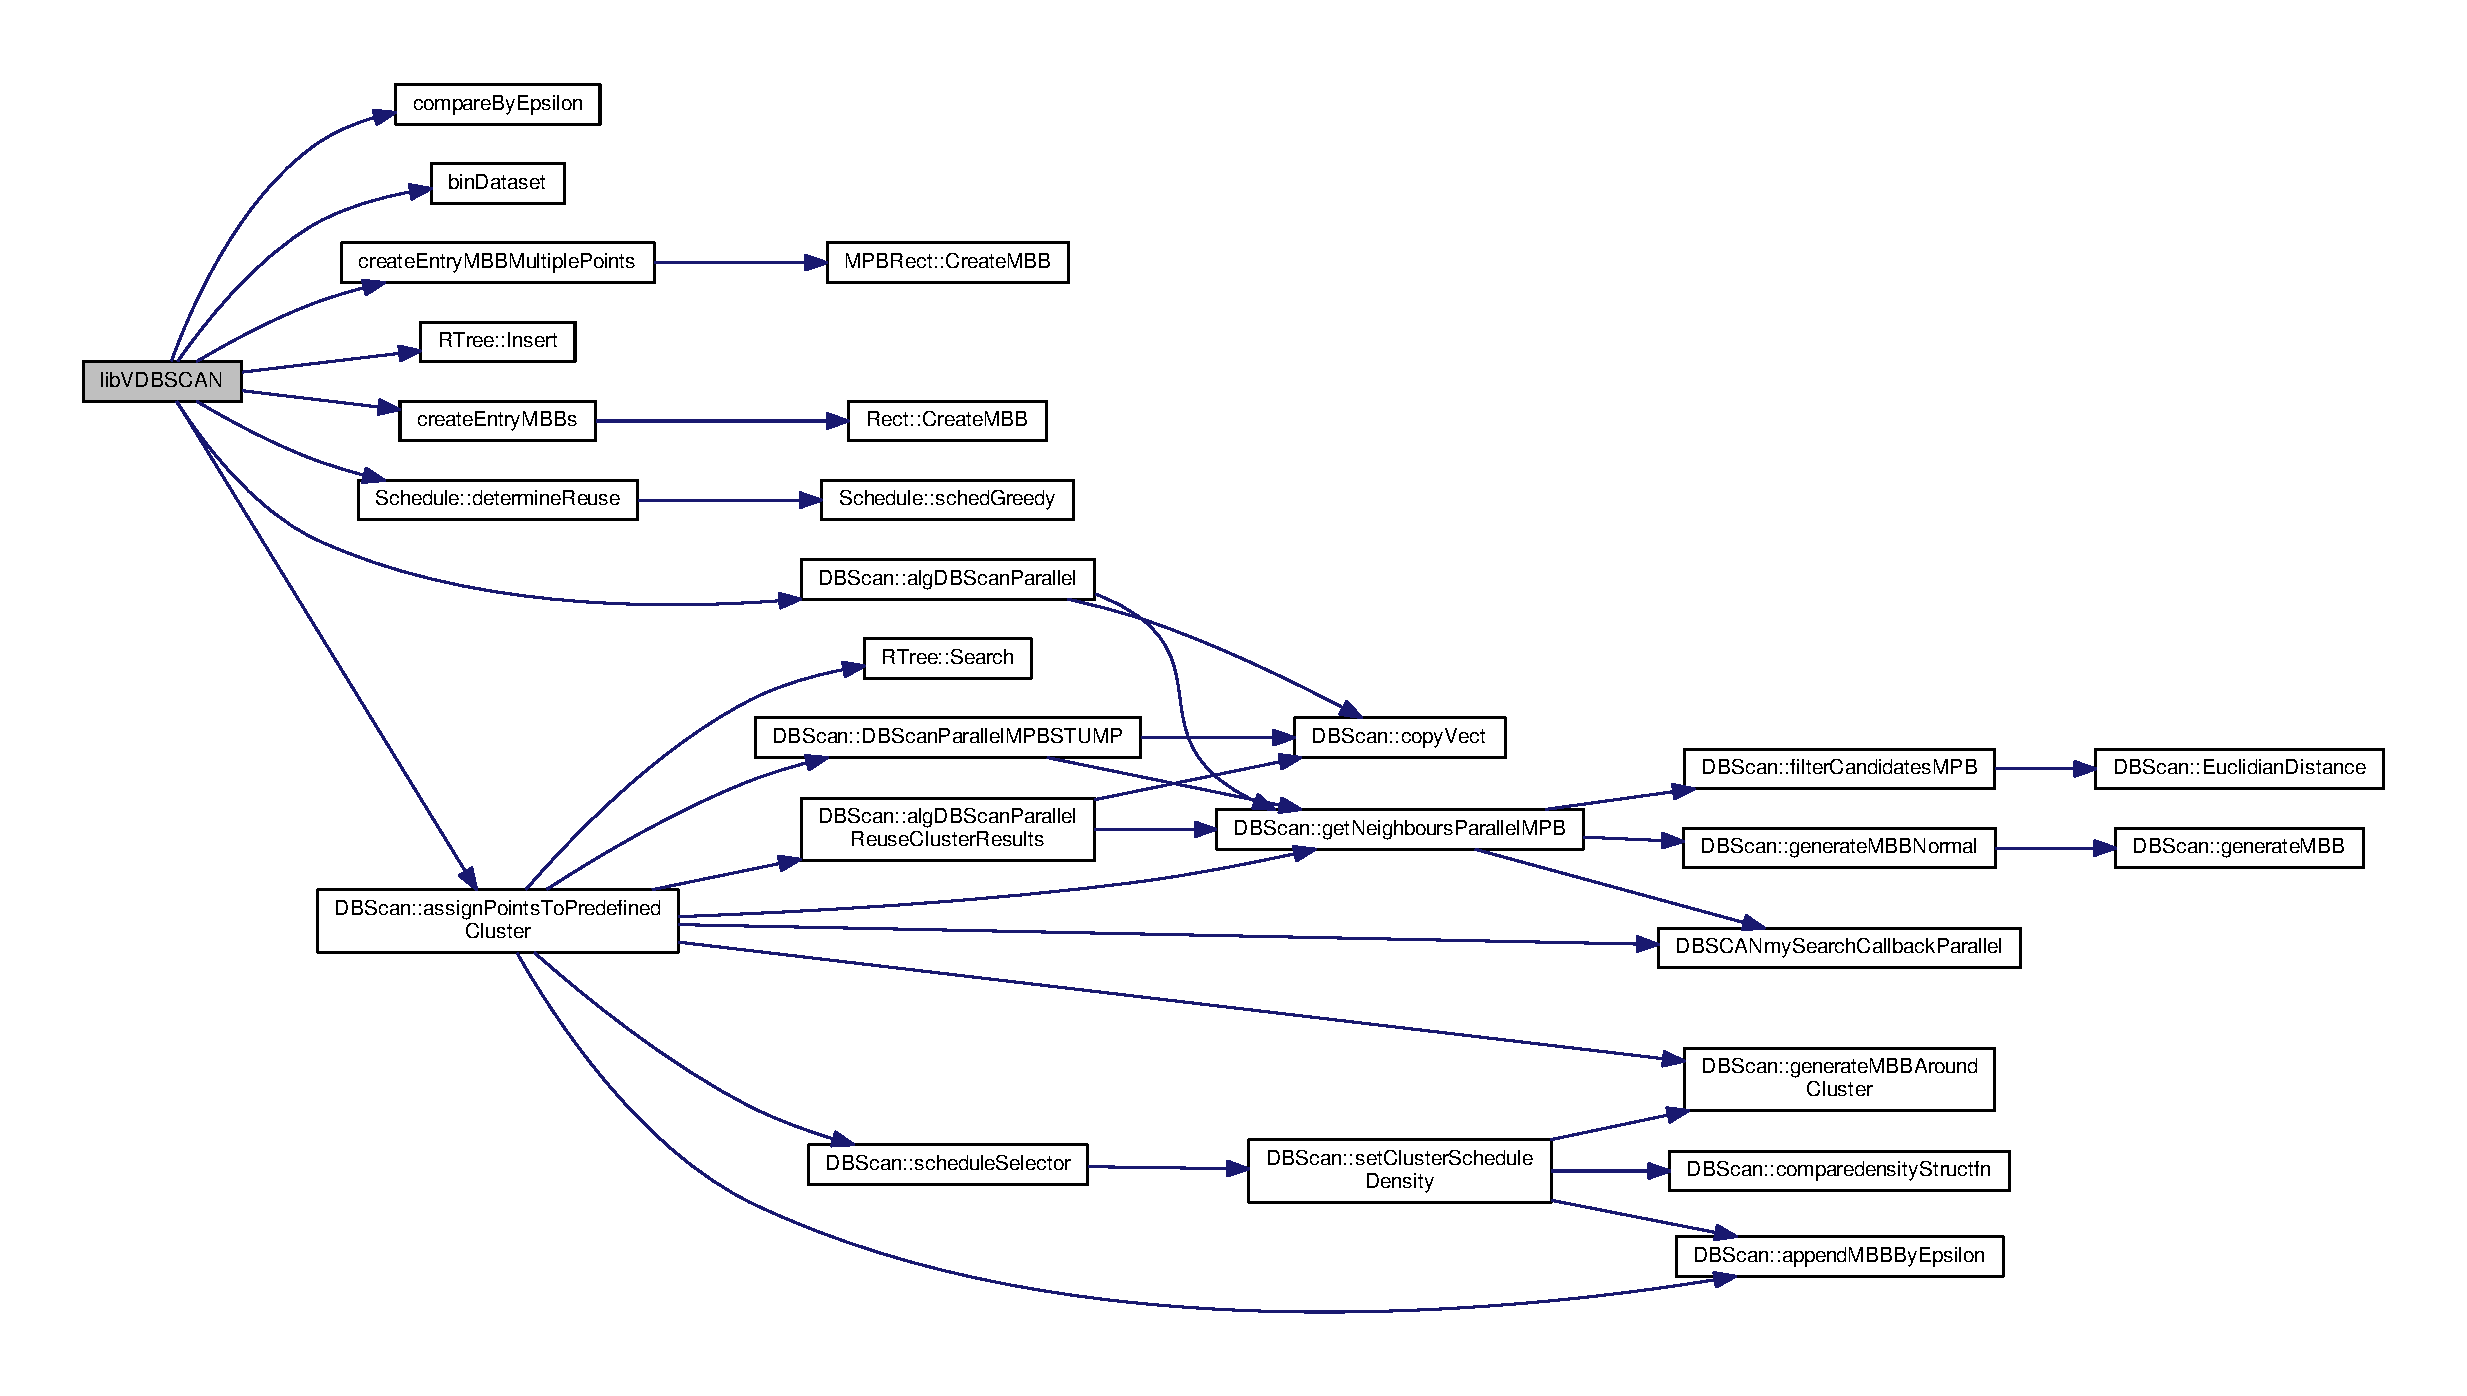
\includegraphics[width=350pt]{main_8cpp_a2a1fa7bbb574f193ee87a385a0c0f06b_cgraph}
\end{center}
\end{figure}



\hypertarget{prototypes_8h}{\section{prototypes.\-h File Reference}
\label{prototypes_8h}\index{prototypes.\-h@{prototypes.\-h}}
}
{\ttfamily \#include \char`\"{}structs.\-h\char`\"{}}\\*
{\ttfamily \#include $<$vector$>$}\\*
Include dependency graph for prototypes.\-h\-:\nopagebreak
\begin{figure}[H]
\begin{center}
\leavevmode
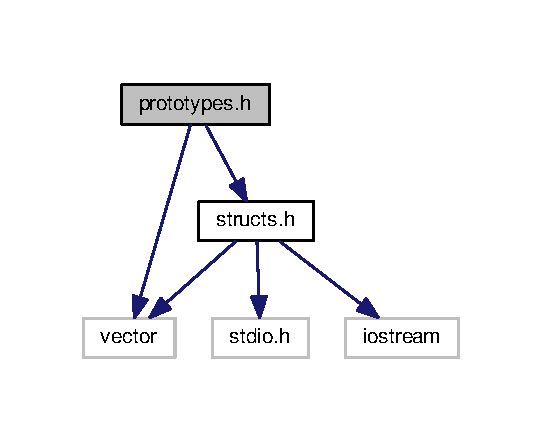
\includegraphics[width=260pt]{prototypes_8h__incl}
\end{center}
\end{figure}
This graph shows which files directly or indirectly include this file\-:\nopagebreak
\begin{figure}[H]
\begin{center}
\leavevmode
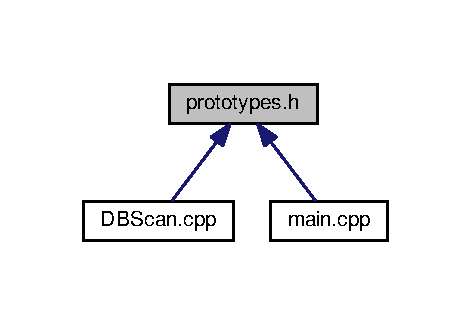
\includegraphics[width=226pt]{prototypes_8h__dep__incl}
\end{center}
\end{figure}
\subsection*{Functions}
\begin{DoxyCompactItemize}
\item 
void \hyperlink{prototypes_8h_a2bbda178e99c2ca95a058f0a26fd2b5d}{import\-Dataset} (std\-::vector$<$ \hyperlink{structdataElem}{data\-Elem} $>$ $\ast$\hyperlink{globals_8h_ac152ac2be0eb07c2b73b4bb54a8f1952}{data\-Points}, char $\ast$fname)
\begin{DoxyCompactList}\small\item\em Imports the 2-\/\-D dataset. \end{DoxyCompactList}\item 
void \hyperlink{prototypes_8h_a8c639584f626e061f0aead36ffa60038}{create\-Entry\-M\-B\-Bs} (std\-::vector$<$ \hyperlink{structdataElem}{data\-Elem} $>$ $\ast$\hyperlink{globals_8h_ac152ac2be0eb07c2b73b4bb54a8f1952}{data\-Points}, \hyperlink{structRect}{Rect} $\ast$data\-Rects)
\begin{DoxyCompactList}\small\item\em Generates M\-B\-Bs for the R-\/tree. \end{DoxyCompactList}\item 
bool \hyperlink{prototypes_8h_a7fecd955d0dfe6edde6077a0f61f950d}{D\-B\-S\-C\-A\-Nmy\-Search\-Callback\-Parallel} (int id, void $\ast$arg)
\begin{DoxyCompactList}\small\item\em Callback function for the R-\/tree. \end{DoxyCompactList}\item 
bool \hyperlink{prototypes_8h_acd7e170375eea7e22e77c1b85f2636bf}{compare\-Data\-Elem\-Struct\-Func} (const \hyperlink{structdataElem}{data\-Elem} \&elem1, const \hyperlink{structdataElem}{data\-Elem} \&elem2)
\begin{DoxyCompactList}\small\item\em Comparison function for sorting. \end{DoxyCompactList}\item 
void \hyperlink{prototypes_8h_a3696e685d39adcfd04cb6c0fe3dd8f74}{create\-Entry\-M\-B\-B\-Multiple\-Points} (std\-::vector$<$ \hyperlink{structdataElem}{data\-Elem} $>$ $\ast$\hyperlink{globals_8h_ac152ac2be0eb07c2b73b4bb54a8f1952}{data\-Points}, std\-::vector$<$ std\-::vector$<$ int $>$ $>$ $\ast$M\-P\-B\-\_\-ids, \hyperlink{structMPBRect}{M\-P\-B\-Rect} $\ast$data\-Rects\-M\-P\-B, int M\-B\-Bsize)
\begin{DoxyCompactList}\small\item\em Generates M\-B\-Bs for for the R-\/tree when indexing multiple points per M\-B\-B. \end{DoxyCompactList}\item 
void \hyperlink{prototypes_8h_a0af007893621bf1d6cb062c927444aa5}{import\-D\-B\-Scan\-Instances} (std\-::vector$<$ struct \hyperlink{structexperiment}{experiment} $>$ $\ast$exper, char $\ast$fname)
\begin{DoxyCompactList}\small\item\em Imports the list of D\-B\-S\-C\-A\-N instances (not used in the shared library version) \end{DoxyCompactList}\item 
bool \hyperlink{prototypes_8h_a786d2eaac37700e364631015ca72e846}{compare\-By\-Epsilon} (const \hyperlink{structexperiment}{experiment} \&a, const \hyperlink{structexperiment}{experiment} \&b)
\begin{DoxyCompactList}\small\item\em Comparison function for sorting. \end{DoxyCompactList}\item 
int \hyperlink{prototypes_8h_ab6302c1085a6ee3030e2a1fa2125e07b}{bin\-\_\-x} (double x)
\begin{DoxyCompactList}\small\item\em Used for binning the input dataset. \end{DoxyCompactList}\item 
int \hyperlink{prototypes_8h_a1b8bf045673fe0bbea47084f6ae126eb}{bin\-\_\-y} (double x)
\begin{DoxyCompactList}\small\item\em Used for binning the input dataset. \end{DoxyCompactList}\item 
void \hyperlink{prototypes_8h_a6ad8dcc1d9af410f2f4640967a4620a6}{bin\-Dataset} (std\-::vector$<$ \hyperlink{structdataElem}{data\-Elem} $>$ $\ast$\hyperlink{globals_8h_ac152ac2be0eb07c2b73b4bb54a8f1952}{data\-Points}, int num\-Bins, std\-::vector$<$ int $>$ $\ast$mapping, bool verbose)
\begin{DoxyCompactList}\small\item\em Bins the 2-\/\-D input dataset, and keeps track of where the points in space were mapped to the original input dataset. \end{DoxyCompactList}\end{DoxyCompactItemize}


\subsection{Function Documentation}
\hypertarget{prototypes_8h_ab6302c1085a6ee3030e2a1fa2125e07b}{\index{prototypes.\-h@{prototypes.\-h}!bin\-\_\-x@{bin\-\_\-x}}
\index{bin\-\_\-x@{bin\-\_\-x}!prototypes.h@{prototypes.\-h}}
\subsubsection[{bin\-\_\-x}]{\setlength{\rightskip}{0pt plus 5cm}int bin\-\_\-x (
\begin{DoxyParamCaption}
\item[{double}]{x}
\end{DoxyParamCaption}
)}}\label{prototypes_8h_ab6302c1085a6ee3030e2a1fa2125e07b}


Used for binning the input dataset. 

\hypertarget{prototypes_8h_a1b8bf045673fe0bbea47084f6ae126eb}{\index{prototypes.\-h@{prototypes.\-h}!bin\-\_\-y@{bin\-\_\-y}}
\index{bin\-\_\-y@{bin\-\_\-y}!prototypes.h@{prototypes.\-h}}
\subsubsection[{bin\-\_\-y}]{\setlength{\rightskip}{0pt plus 5cm}int bin\-\_\-y (
\begin{DoxyParamCaption}
\item[{double}]{x}
\end{DoxyParamCaption}
)}}\label{prototypes_8h_a1b8bf045673fe0bbea47084f6ae126eb}


Used for binning the input dataset. 

\hypertarget{prototypes_8h_a6ad8dcc1d9af410f2f4640967a4620a6}{\index{prototypes.\-h@{prototypes.\-h}!bin\-Dataset@{bin\-Dataset}}
\index{bin\-Dataset@{bin\-Dataset}!prototypes.h@{prototypes.\-h}}
\subsubsection[{bin\-Dataset}]{\setlength{\rightskip}{0pt plus 5cm}void bin\-Dataset (
\begin{DoxyParamCaption}
\item[{std\-::vector$<$ {\bf data\-Elem} $>$ $\ast$}]{data\-Points, }
\item[{int}]{num\-Bins, }
\item[{std\-::vector$<$ int $>$ $\ast$}]{mapping, }
\item[{bool}]{verbose}
\end{DoxyParamCaption}
)}}\label{prototypes_8h_a6ad8dcc1d9af410f2f4640967a4620a6}


Bins the 2-\/\-D input dataset, and keeps track of where the points in space were mapped to the original input dataset. 

\hypertarget{prototypes_8h_a786d2eaac37700e364631015ca72e846}{\index{prototypes.\-h@{prototypes.\-h}!compare\-By\-Epsilon@{compare\-By\-Epsilon}}
\index{compare\-By\-Epsilon@{compare\-By\-Epsilon}!prototypes.h@{prototypes.\-h}}
\subsubsection[{compare\-By\-Epsilon}]{\setlength{\rightskip}{0pt plus 5cm}bool compare\-By\-Epsilon (
\begin{DoxyParamCaption}
\item[{const {\bf experiment} \&}]{a, }
\item[{const {\bf experiment} \&}]{b}
\end{DoxyParamCaption}
)}}\label{prototypes_8h_a786d2eaac37700e364631015ca72e846}


Comparison function for sorting. 

\hypertarget{prototypes_8h_acd7e170375eea7e22e77c1b85f2636bf}{\index{prototypes.\-h@{prototypes.\-h}!compare\-Data\-Elem\-Struct\-Func@{compare\-Data\-Elem\-Struct\-Func}}
\index{compare\-Data\-Elem\-Struct\-Func@{compare\-Data\-Elem\-Struct\-Func}!prototypes.h@{prototypes.\-h}}
\subsubsection[{compare\-Data\-Elem\-Struct\-Func}]{\setlength{\rightskip}{0pt plus 5cm}bool compare\-Data\-Elem\-Struct\-Func (
\begin{DoxyParamCaption}
\item[{const {\bf data\-Elem} \&}]{elem1, }
\item[{const {\bf data\-Elem} \&}]{elem2}
\end{DoxyParamCaption}
)}}\label{prototypes_8h_acd7e170375eea7e22e77c1b85f2636bf}


Comparison function for sorting. 



Here is the call graph for this function\-:
\nopagebreak
\begin{figure}[H]
\begin{center}
\leavevmode
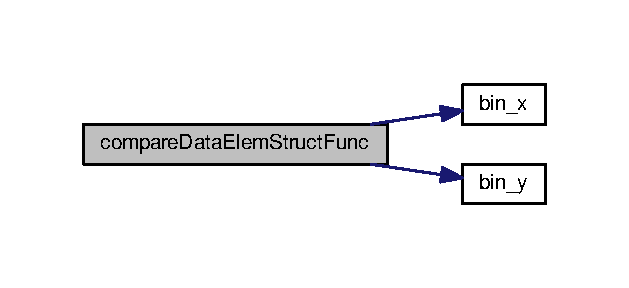
\includegraphics[width=302pt]{prototypes_8h_acd7e170375eea7e22e77c1b85f2636bf_cgraph}
\end{center}
\end{figure}


\hypertarget{prototypes_8h_a3696e685d39adcfd04cb6c0fe3dd8f74}{\index{prototypes.\-h@{prototypes.\-h}!create\-Entry\-M\-B\-B\-Multiple\-Points@{create\-Entry\-M\-B\-B\-Multiple\-Points}}
\index{create\-Entry\-M\-B\-B\-Multiple\-Points@{create\-Entry\-M\-B\-B\-Multiple\-Points}!prototypes.h@{prototypes.\-h}}
\subsubsection[{create\-Entry\-M\-B\-B\-Multiple\-Points}]{\setlength{\rightskip}{0pt plus 5cm}void create\-Entry\-M\-B\-B\-Multiple\-Points (
\begin{DoxyParamCaption}
\item[{std\-::vector$<$ {\bf data\-Elem} $>$ $\ast$}]{data\-Points, }
\item[{std\-::vector$<$ std\-::vector$<$ int $>$ $>$ $\ast$}]{M\-P\-B\-\_\-ids, }
\item[{{\bf M\-P\-B\-Rect} $\ast$}]{data\-Rects\-M\-P\-B, }
\item[{int}]{M\-B\-Bsize}
\end{DoxyParamCaption}
)}}\label{prototypes_8h_a3696e685d39adcfd04cb6c0fe3dd8f74}


Generates M\-B\-Bs for for the R-\/tree when indexing multiple points per M\-B\-B. 



Here is the call graph for this function\-:\nopagebreak
\begin{figure}[H]
\begin{center}
\leavevmode
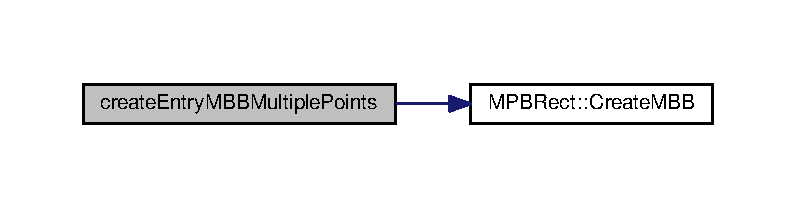
\includegraphics[width=350pt]{prototypes_8h_a3696e685d39adcfd04cb6c0fe3dd8f74_cgraph}
\end{center}
\end{figure}


\hypertarget{prototypes_8h_a8c639584f626e061f0aead36ffa60038}{\index{prototypes.\-h@{prototypes.\-h}!create\-Entry\-M\-B\-Bs@{create\-Entry\-M\-B\-Bs}}
\index{create\-Entry\-M\-B\-Bs@{create\-Entry\-M\-B\-Bs}!prototypes.h@{prototypes.\-h}}
\subsubsection[{create\-Entry\-M\-B\-Bs}]{\setlength{\rightskip}{0pt plus 5cm}void create\-Entry\-M\-B\-Bs (
\begin{DoxyParamCaption}
\item[{std\-::vector$<$ {\bf data\-Elem} $>$ $\ast$}]{data\-Points, }
\item[{{\bf Rect} $\ast$}]{data\-Rects}
\end{DoxyParamCaption}
)}}\label{prototypes_8h_a8c639584f626e061f0aead36ffa60038}


Generates M\-B\-Bs for the R-\/tree. 



Here is the call graph for this function\-:\nopagebreak
\begin{figure}[H]
\begin{center}
\leavevmode
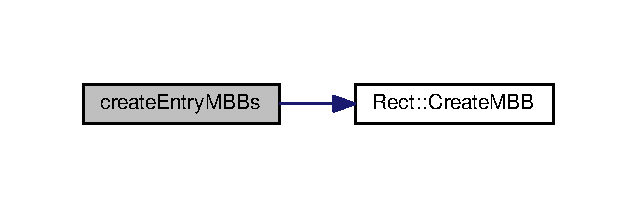
\includegraphics[width=306pt]{prototypes_8h_a8c639584f626e061f0aead36ffa60038_cgraph}
\end{center}
\end{figure}


\hypertarget{prototypes_8h_a7fecd955d0dfe6edde6077a0f61f950d}{\index{prototypes.\-h@{prototypes.\-h}!D\-B\-S\-C\-A\-Nmy\-Search\-Callback\-Parallel@{D\-B\-S\-C\-A\-Nmy\-Search\-Callback\-Parallel}}
\index{D\-B\-S\-C\-A\-Nmy\-Search\-Callback\-Parallel@{D\-B\-S\-C\-A\-Nmy\-Search\-Callback\-Parallel}!prototypes.h@{prototypes.\-h}}
\subsubsection[{D\-B\-S\-C\-A\-Nmy\-Search\-Callback\-Parallel}]{\setlength{\rightskip}{0pt plus 5cm}bool D\-B\-S\-C\-A\-Nmy\-Search\-Callback\-Parallel (
\begin{DoxyParamCaption}
\item[{int}]{id, }
\item[{void $\ast$}]{arg}
\end{DoxyParamCaption}
)}}\label{prototypes_8h_a7fecd955d0dfe6edde6077a0f61f950d}


Callback function for the R-\/tree. 

\hypertarget{prototypes_8h_a2bbda178e99c2ca95a058f0a26fd2b5d}{\index{prototypes.\-h@{prototypes.\-h}!import\-Dataset@{import\-Dataset}}
\index{import\-Dataset@{import\-Dataset}!prototypes.h@{prototypes.\-h}}
\subsubsection[{import\-Dataset}]{\setlength{\rightskip}{0pt plus 5cm}void import\-Dataset (
\begin{DoxyParamCaption}
\item[{std\-::vector$<$ {\bf data\-Elem} $>$ $\ast$}]{data\-Points, }
\item[{char $\ast$}]{fname}
\end{DoxyParamCaption}
)}}\label{prototypes_8h_a2bbda178e99c2ca95a058f0a26fd2b5d}


Imports the 2-\/\-D dataset. 

\hypertarget{prototypes_8h_a0af007893621bf1d6cb062c927444aa5}{\index{prototypes.\-h@{prototypes.\-h}!import\-D\-B\-Scan\-Instances@{import\-D\-B\-Scan\-Instances}}
\index{import\-D\-B\-Scan\-Instances@{import\-D\-B\-Scan\-Instances}!prototypes.h@{prototypes.\-h}}
\subsubsection[{import\-D\-B\-Scan\-Instances}]{\setlength{\rightskip}{0pt plus 5cm}void import\-D\-B\-Scan\-Instances (
\begin{DoxyParamCaption}
\item[{std\-::vector$<$ struct {\bf experiment} $>$ $\ast$}]{exper, }
\item[{char $\ast$}]{fname}
\end{DoxyParamCaption}
)}}\label{prototypes_8h_a0af007893621bf1d6cb062c927444aa5}


Imports the list of D\-B\-S\-C\-A\-N instances (not used in the shared library version) 


\hypertarget{RTree_8h}{\section{R\-Tree.\-h File Reference}
\label{RTree_8h}\index{R\-Tree.\-h@{R\-Tree.\-h}}
}
{\ttfamily \#include $<$stdio.\-h$>$}\\*
{\ttfamily \#include $<$math.\-h$>$}\\*
{\ttfamily \#include $<$assert.\-h$>$}\\*
{\ttfamily \#include $<$stdlib.\-h$>$}\\*
{\ttfamily \#include $<$algorithm$>$}\\*
Include dependency graph for R\-Tree.\-h\-:\nopagebreak
\begin{figure}[H]
\begin{center}
\leavevmode
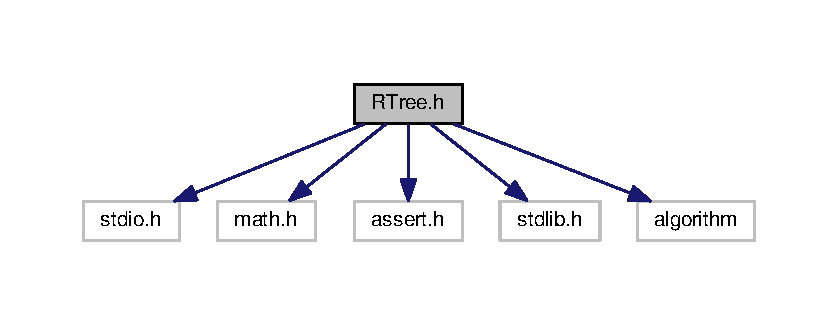
\includegraphics[width=350pt]{RTree_8h__incl}
\end{center}
\end{figure}
This graph shows which files directly or indirectly include this file\-:\nopagebreak
\begin{figure}[H]
\begin{center}
\leavevmode
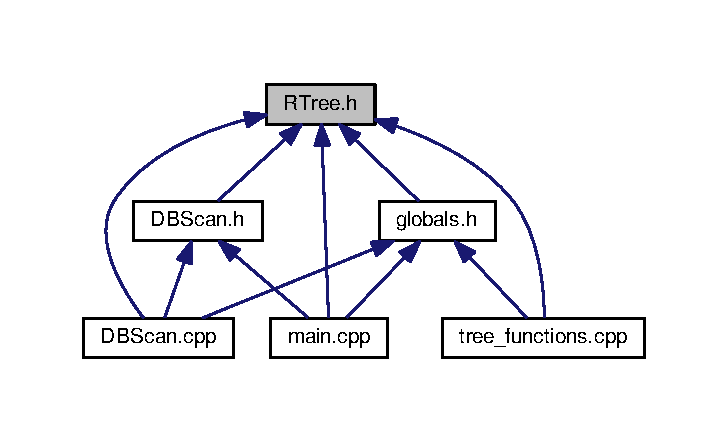
\includegraphics[width=349pt]{RTree_8h__dep__incl}
\end{center}
\end{figure}
\subsection*{Data Structures}
\begin{DoxyCompactItemize}
\item 
class \hyperlink{classRTree}{R\-Tree$<$ D\-A\-T\-A\-T\-Y\-P\-E, E\-L\-E\-M\-T\-Y\-P\-E, N\-U\-M\-D\-I\-M\-S, E\-L\-E\-M\-T\-Y\-P\-E\-R\-E\-A\-L, T\-M\-A\-X\-N\-O\-D\-E\-S, T\-M\-I\-N\-N\-O\-D\-E\-S $>$}
\item 
class \hyperlink{classRTree_1_1Iterator}{R\-Tree$<$ D\-A\-T\-A\-T\-Y\-P\-E, E\-L\-E\-M\-T\-Y\-P\-E, N\-U\-M\-D\-I\-M\-S, E\-L\-E\-M\-T\-Y\-P\-E\-R\-E\-A\-L, T\-M\-A\-X\-N\-O\-D\-E\-S, T\-M\-I\-N\-N\-O\-D\-E\-S $>$\-::\-Iterator}
\begin{DoxyCompactList}\small\item\em \hyperlink{classRTree_1_1Iterator}{Iterator} is not remove safe. \end{DoxyCompactList}\item 
struct \hyperlink{structRTree_1_1Iterator_1_1StackElement}{R\-Tree$<$ D\-A\-T\-A\-T\-Y\-P\-E, E\-L\-E\-M\-T\-Y\-P\-E, N\-U\-M\-D\-I\-M\-S, E\-L\-E\-M\-T\-Y\-P\-E\-R\-E\-A\-L, T\-M\-A\-X\-N\-O\-D\-E\-S, T\-M\-I\-N\-N\-O\-D\-E\-S $>$\-::\-Iterator\-::\-Stack\-Element}
\item 
struct \hyperlink{structRTree_1_1Rect}{R\-Tree$<$ D\-A\-T\-A\-T\-Y\-P\-E, E\-L\-E\-M\-T\-Y\-P\-E, N\-U\-M\-D\-I\-M\-S, E\-L\-E\-M\-T\-Y\-P\-E\-R\-E\-A\-L, T\-M\-A\-X\-N\-O\-D\-E\-S, T\-M\-I\-N\-N\-O\-D\-E\-S $>$\-::\-Rect}
\begin{DoxyCompactList}\small\item\em Minimal bounding rectangle (n-\/dimensional) \end{DoxyCompactList}\item 
struct \hyperlink{structRTree_1_1Branch}{R\-Tree$<$ D\-A\-T\-A\-T\-Y\-P\-E, E\-L\-E\-M\-T\-Y\-P\-E, N\-U\-M\-D\-I\-M\-S, E\-L\-E\-M\-T\-Y\-P\-E\-R\-E\-A\-L, T\-M\-A\-X\-N\-O\-D\-E\-S, T\-M\-I\-N\-N\-O\-D\-E\-S $>$\-::\-Branch}
\item 
struct \hyperlink{structRTree_1_1Node}{R\-Tree$<$ D\-A\-T\-A\-T\-Y\-P\-E, E\-L\-E\-M\-T\-Y\-P\-E, N\-U\-M\-D\-I\-M\-S, E\-L\-E\-M\-T\-Y\-P\-E\-R\-E\-A\-L, T\-M\-A\-X\-N\-O\-D\-E\-S, T\-M\-I\-N\-N\-O\-D\-E\-S $>$\-::\-Node}
\begin{DoxyCompactList}\small\item\em \hyperlink{structRTree_1_1Node}{Node} for each branch level. \end{DoxyCompactList}\item 
struct \hyperlink{structRTree_1_1ListNode}{R\-Tree$<$ D\-A\-T\-A\-T\-Y\-P\-E, E\-L\-E\-M\-T\-Y\-P\-E, N\-U\-M\-D\-I\-M\-S, E\-L\-E\-M\-T\-Y\-P\-E\-R\-E\-A\-L, T\-M\-A\-X\-N\-O\-D\-E\-S, T\-M\-I\-N\-N\-O\-D\-E\-S $>$\-::\-List\-Node}
\begin{DoxyCompactList}\small\item\em A link list of nodes for reinsertion after a delete operation. \end{DoxyCompactList}\item 
struct \hyperlink{structRTree_1_1PartitionVars}{R\-Tree$<$ D\-A\-T\-A\-T\-Y\-P\-E, E\-L\-E\-M\-T\-Y\-P\-E, N\-U\-M\-D\-I\-M\-S, E\-L\-E\-M\-T\-Y\-P\-E\-R\-E\-A\-L, T\-M\-A\-X\-N\-O\-D\-E\-S, T\-M\-I\-N\-N\-O\-D\-E\-S $>$\-::\-Partition\-Vars}
\begin{DoxyCompactList}\small\item\em Variables for finding a split partition. \end{DoxyCompactList}\item 
class \hyperlink{classRTFileStream}{R\-T\-File\-Stream}
\end{DoxyCompactItemize}
\subsection*{Macros}
\begin{DoxyCompactItemize}
\item 
\#define \hyperlink{RTree_8h_af343b20373ba49a92fce523e948f2ab3}{A\-S\-S\-E\-R\-T}~assert
\item 
\#define \hyperlink{RTree_8h_a86d632fa0bef69c8cc19f84f1683de9e}{Min}~std\-::min
\item 
\#define \hyperlink{RTree_8h_a406ea73ae9534077b145f331cd542401}{Max}~std\-::max
\item 
\#define \hyperlink{RTree_8h_aa9b462b3b7b1c8cda40b182c09eed713}{R\-T\-R\-E\-E\-\_\-\-T\-E\-M\-P\-L\-A\-T\-E}~template$<$class D\-A\-T\-A\-T\-Y\-P\-E, class E\-L\-E\-M\-T\-Y\-P\-E, int N\-U\-M\-D\-I\-M\-S, class E\-L\-E\-M\-T\-Y\-P\-E\-R\-E\-A\-L, int T\-M\-A\-X\-N\-O\-D\-E\-S, int T\-M\-I\-N\-N\-O\-D\-E\-S$>$
\item 
\#define \hyperlink{RTree_8h_a21aed6cfcbda84c4663c90768cefee0b}{R\-T\-R\-E\-E\-\_\-\-Q\-U\-A\-L}~\hyperlink{classRTree}{R\-Tree}$<$D\-A\-T\-A\-T\-Y\-P\-E, E\-L\-E\-M\-T\-Y\-P\-E, N\-U\-M\-D\-I\-M\-S, E\-L\-E\-M\-T\-Y\-P\-E\-R\-E\-A\-L, T\-M\-A\-X\-N\-O\-D\-E\-S, T\-M\-I\-N\-N\-O\-D\-E\-S$>$
\item 
\#define \hyperlink{RTree_8h_a48ab98477536b7144da4b56f4a69af99}{R\-T\-R\-E\-E\-\_\-\-D\-O\-N\-T\-\_\-\-U\-S\-E\-\_\-\-M\-E\-M\-P\-O\-O\-L\-S}
\item 
\#define \hyperlink{RTree_8h_a6f664e156a52787974ce765dd81641f3}{R\-T\-R\-E\-E\-\_\-\-U\-S\-E\-\_\-\-S\-P\-H\-E\-R\-I\-C\-A\-L\-\_\-\-V\-O\-L\-U\-M\-E}
\end{DoxyCompactItemize}


\subsection{Macro Definition Documentation}
\hypertarget{RTree_8h_af343b20373ba49a92fce523e948f2ab3}{\index{R\-Tree.\-h@{R\-Tree.\-h}!A\-S\-S\-E\-R\-T@{A\-S\-S\-E\-R\-T}}
\index{A\-S\-S\-E\-R\-T@{A\-S\-S\-E\-R\-T}!RTree.h@{R\-Tree.\-h}}
\subsubsection[{A\-S\-S\-E\-R\-T}]{\setlength{\rightskip}{0pt plus 5cm}\#define A\-S\-S\-E\-R\-T~assert}}\label{RTree_8h_af343b20373ba49a92fce523e948f2ab3}
\hypertarget{RTree_8h_a406ea73ae9534077b145f331cd542401}{\index{R\-Tree.\-h@{R\-Tree.\-h}!Max@{Max}}
\index{Max@{Max}!RTree.h@{R\-Tree.\-h}}
\subsubsection[{Max}]{\setlength{\rightskip}{0pt plus 5cm}\#define Max~std\-::max}}\label{RTree_8h_a406ea73ae9534077b145f331cd542401}
\hypertarget{RTree_8h_a86d632fa0bef69c8cc19f84f1683de9e}{\index{R\-Tree.\-h@{R\-Tree.\-h}!Min@{Min}}
\index{Min@{Min}!RTree.h@{R\-Tree.\-h}}
\subsubsection[{Min}]{\setlength{\rightskip}{0pt plus 5cm}\#define Min~std\-::min}}\label{RTree_8h_a86d632fa0bef69c8cc19f84f1683de9e}
\hypertarget{RTree_8h_a48ab98477536b7144da4b56f4a69af99}{\index{R\-Tree.\-h@{R\-Tree.\-h}!R\-T\-R\-E\-E\-\_\-\-D\-O\-N\-T\-\_\-\-U\-S\-E\-\_\-\-M\-E\-M\-P\-O\-O\-L\-S@{R\-T\-R\-E\-E\-\_\-\-D\-O\-N\-T\-\_\-\-U\-S\-E\-\_\-\-M\-E\-M\-P\-O\-O\-L\-S}}
\index{R\-T\-R\-E\-E\-\_\-\-D\-O\-N\-T\-\_\-\-U\-S\-E\-\_\-\-M\-E\-M\-P\-O\-O\-L\-S@{R\-T\-R\-E\-E\-\_\-\-D\-O\-N\-T\-\_\-\-U\-S\-E\-\_\-\-M\-E\-M\-P\-O\-O\-L\-S}!RTree.h@{R\-Tree.\-h}}
\subsubsection[{R\-T\-R\-E\-E\-\_\-\-D\-O\-N\-T\-\_\-\-U\-S\-E\-\_\-\-M\-E\-M\-P\-O\-O\-L\-S}]{\setlength{\rightskip}{0pt plus 5cm}\#define R\-T\-R\-E\-E\-\_\-\-D\-O\-N\-T\-\_\-\-U\-S\-E\-\_\-\-M\-E\-M\-P\-O\-O\-L\-S}}\label{RTree_8h_a48ab98477536b7144da4b56f4a69af99}
\hypertarget{RTree_8h_a21aed6cfcbda84c4663c90768cefee0b}{\index{R\-Tree.\-h@{R\-Tree.\-h}!R\-T\-R\-E\-E\-\_\-\-Q\-U\-A\-L@{R\-T\-R\-E\-E\-\_\-\-Q\-U\-A\-L}}
\index{R\-T\-R\-E\-E\-\_\-\-Q\-U\-A\-L@{R\-T\-R\-E\-E\-\_\-\-Q\-U\-A\-L}!RTree.h@{R\-Tree.\-h}}
\subsubsection[{R\-T\-R\-E\-E\-\_\-\-Q\-U\-A\-L}]{\setlength{\rightskip}{0pt plus 5cm}\#define R\-T\-R\-E\-E\-\_\-\-Q\-U\-A\-L~{\bf R\-Tree}$<$D\-A\-T\-A\-T\-Y\-P\-E, E\-L\-E\-M\-T\-Y\-P\-E, N\-U\-M\-D\-I\-M\-S, E\-L\-E\-M\-T\-Y\-P\-E\-R\-E\-A\-L, T\-M\-A\-X\-N\-O\-D\-E\-S, T\-M\-I\-N\-N\-O\-D\-E\-S$>$}}\label{RTree_8h_a21aed6cfcbda84c4663c90768cefee0b}
\hypertarget{RTree_8h_aa9b462b3b7b1c8cda40b182c09eed713}{\index{R\-Tree.\-h@{R\-Tree.\-h}!R\-T\-R\-E\-E\-\_\-\-T\-E\-M\-P\-L\-A\-T\-E@{R\-T\-R\-E\-E\-\_\-\-T\-E\-M\-P\-L\-A\-T\-E}}
\index{R\-T\-R\-E\-E\-\_\-\-T\-E\-M\-P\-L\-A\-T\-E@{R\-T\-R\-E\-E\-\_\-\-T\-E\-M\-P\-L\-A\-T\-E}!RTree.h@{R\-Tree.\-h}}
\subsubsection[{R\-T\-R\-E\-E\-\_\-\-T\-E\-M\-P\-L\-A\-T\-E}]{\setlength{\rightskip}{0pt plus 5cm}\#define R\-T\-R\-E\-E\-\_\-\-T\-E\-M\-P\-L\-A\-T\-E~template$<$class D\-A\-T\-A\-T\-Y\-P\-E, class E\-L\-E\-M\-T\-Y\-P\-E, int N\-U\-M\-D\-I\-M\-S, class E\-L\-E\-M\-T\-Y\-P\-E\-R\-E\-A\-L, int T\-M\-A\-X\-N\-O\-D\-E\-S, int T\-M\-I\-N\-N\-O\-D\-E\-S$>$}}\label{RTree_8h_aa9b462b3b7b1c8cda40b182c09eed713}
\hypertarget{RTree_8h_a6f664e156a52787974ce765dd81641f3}{\index{R\-Tree.\-h@{R\-Tree.\-h}!R\-T\-R\-E\-E\-\_\-\-U\-S\-E\-\_\-\-S\-P\-H\-E\-R\-I\-C\-A\-L\-\_\-\-V\-O\-L\-U\-M\-E@{R\-T\-R\-E\-E\-\_\-\-U\-S\-E\-\_\-\-S\-P\-H\-E\-R\-I\-C\-A\-L\-\_\-\-V\-O\-L\-U\-M\-E}}
\index{R\-T\-R\-E\-E\-\_\-\-U\-S\-E\-\_\-\-S\-P\-H\-E\-R\-I\-C\-A\-L\-\_\-\-V\-O\-L\-U\-M\-E@{R\-T\-R\-E\-E\-\_\-\-U\-S\-E\-\_\-\-S\-P\-H\-E\-R\-I\-C\-A\-L\-\_\-\-V\-O\-L\-U\-M\-E}!RTree.h@{R\-Tree.\-h}}
\subsubsection[{R\-T\-R\-E\-E\-\_\-\-U\-S\-E\-\_\-\-S\-P\-H\-E\-R\-I\-C\-A\-L\-\_\-\-V\-O\-L\-U\-M\-E}]{\setlength{\rightskip}{0pt plus 5cm}\#define R\-T\-R\-E\-E\-\_\-\-U\-S\-E\-\_\-\-S\-P\-H\-E\-R\-I\-C\-A\-L\-\_\-\-V\-O\-L\-U\-M\-E}}\label{RTree_8h_a6f664e156a52787974ce765dd81641f3}

\hypertarget{schedule_8cpp}{\section{schedule.\-cpp File Reference}
\label{schedule_8cpp}\index{schedule.\-cpp@{schedule.\-cpp}}
}
{\ttfamily \#include \char`\"{}schedule.\-h\char`\"{}}\\*
{\ttfamily \#include $<$omp.\-h$>$}\\*
{\ttfamily \#include $<$vector$>$}\\*
{\ttfamily \#include $<$algorithm$>$}\\*
Include dependency graph for schedule.\-cpp\-:\nopagebreak
\begin{figure}[H]
\begin{center}
\leavevmode
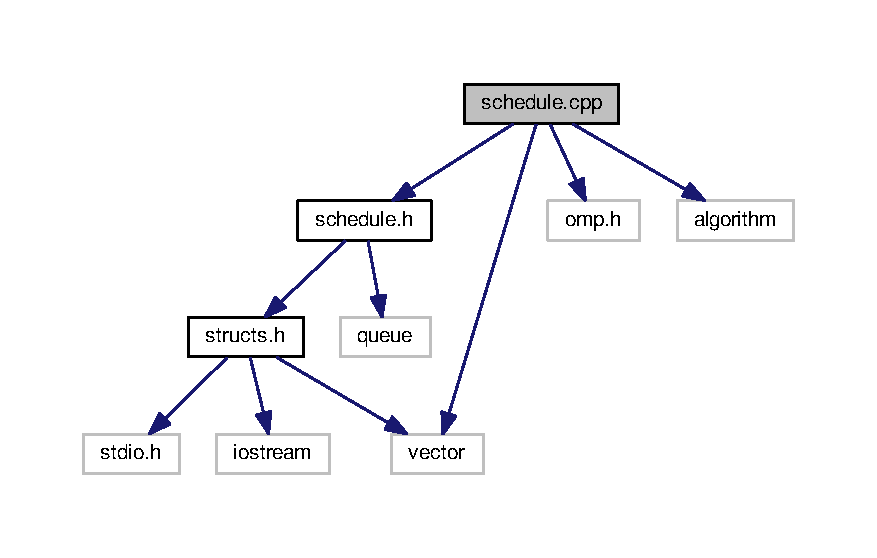
\includegraphics[width=350pt]{schedule_8cpp__incl}
\end{center}
\end{figure}

\hypertarget{schedule_8h}{\section{schedule.\-h File Reference}
\label{schedule_8h}\index{schedule.\-h@{schedule.\-h}}
}
{\ttfamily \#include \char`\"{}structs.\-h\char`\"{}}\\*
{\ttfamily \#include $<$queue$>$}\\*
Include dependency graph for schedule.\-h\-:\nopagebreak
\begin{figure}[H]
\begin{center}
\leavevmode
\includegraphics[width=260pt]{schedule_8h__incl}
\end{center}
\end{figure}
This graph shows which files directly or indirectly include this file\-:\nopagebreak
\begin{figure}[H]
\begin{center}
\leavevmode
\includegraphics[width=228pt]{schedule_8h__dep__incl}
\end{center}
\end{figure}
\subsection*{Data Structures}
\begin{DoxyCompactItemize}
\item 
class \hyperlink{classSchedule}{Schedule}
\end{DoxyCompactItemize}

\hypertarget{structs_8h}{\section{structs.\-h File Reference}
\label{structs_8h}\index{structs.\-h@{structs.\-h}}
}
{\ttfamily \#include $<$vector$>$}\\*
{\ttfamily \#include $<$stdio.\-h$>$}\\*
{\ttfamily \#include $<$iostream$>$}\\*
Include dependency graph for structs.\-h\-:\nopagebreak
\begin{figure}[H]
\begin{center}
\leavevmode
\includegraphics[width=260pt]{structs_8h__incl}
\end{center}
\end{figure}
This graph shows which files directly or indirectly include this file\-:\nopagebreak
\begin{figure}[H]
\begin{center}
\leavevmode
\includegraphics[width=350pt]{structs_8h__dep__incl}
\end{center}
\end{figure}
\subsection*{Data Structures}
\begin{DoxyCompactItemize}
\item 
struct \hyperlink{structexperiment}{experiment}
\item 
struct \hyperlink{structschedInfo}{sched\-Info}
\item 
struct \hyperlink{structdataElem}{data\-Elem}
\item 
struct \hyperlink{structdensityStruct}{density\-Struct}
\item 
struct \hyperlink{structMPBRect}{M\-P\-B\-Rect}
\item 
struct \hyperlink{structRect}{Rect}
\item 
struct \hyperlink{structQueryRect}{Query\-Rect}
\end{DoxyCompactItemize}

\hypertarget{tree__functions_8cpp}{\section{tree\-\_\-functions.\-cpp File Reference}
\label{tree__functions_8cpp}\index{tree\-\_\-functions.\-cpp@{tree\-\_\-functions.\-cpp}}
}
{\ttfamily \#include \char`\"{}R\-Tree.\-h\char`\"{}}\\*
{\ttfamily \#include \char`\"{}globals.\-h\char`\"{}}\\*
{\ttfamily \#include $<$omp.\-h$>$}\\*
{\ttfamily \#include $<$stdlib.\-h$>$}\\*
Include dependency graph for tree\-\_\-functions.\-cpp\-:\nopagebreak
\begin{figure}[H]
\begin{center}
\leavevmode
\includegraphics[width=350pt]{tree__functions_8cpp__incl}
\end{center}
\end{figure}
\subsection*{Functions}
\begin{DoxyCompactItemize}
\item 
bool \hyperlink{tree__functions_8cpp_a7fecd955d0dfe6edde6077a0f61f950d}{D\-B\-S\-C\-A\-Nmy\-Search\-Callback\-Parallel} (int id, void $\ast$arg)
\begin{DoxyCompactList}\small\item\em Callback function for the R-\/tree. \end{DoxyCompactList}\end{DoxyCompactItemize}


\subsection{Function Documentation}
\hypertarget{tree__functions_8cpp_a7fecd955d0dfe6edde6077a0f61f950d}{\index{tree\-\_\-functions.\-cpp@{tree\-\_\-functions.\-cpp}!D\-B\-S\-C\-A\-Nmy\-Search\-Callback\-Parallel@{D\-B\-S\-C\-A\-Nmy\-Search\-Callback\-Parallel}}
\index{D\-B\-S\-C\-A\-Nmy\-Search\-Callback\-Parallel@{D\-B\-S\-C\-A\-Nmy\-Search\-Callback\-Parallel}!tree_functions.cpp@{tree\-\_\-functions.\-cpp}}
\subsubsection[{D\-B\-S\-C\-A\-Nmy\-Search\-Callback\-Parallel}]{\setlength{\rightskip}{0pt plus 5cm}bool D\-B\-S\-C\-A\-Nmy\-Search\-Callback\-Parallel (
\begin{DoxyParamCaption}
\item[{int}]{id, }
\item[{void $\ast$}]{arg}
\end{DoxyParamCaption}
)}}\label{tree__functions_8cpp_a7fecd955d0dfe6edde6077a0f61f950d}


Callback function for the R-\/tree. 


%--- End generated contents ---

% Index
\newpage
\phantomsection
\addcontentsline{toc}{chapter}{Index}
\printindex

\end{document}
